% !TEX program = xelatex
\documentclass[UTF8,fontset=fandol,a4paper,11pt]{ctexart}
\usepackage[margin=21mm,top=23mm,bottom=22mm,headheight=16pt]{geometry}
\usepackage{amsmath,amssymb,mathtools,bm}
\usepackage{tikz}
\usetikzlibrary{arrows.meta,calc,angles,quotes,patterns}
\usepackage{xcolor,booktabs,array,longtable,enumitem,fancyhdr,needspace}
\usepackage[unicode,hidelinks]{hyperref}
\definecolor{ink}{HTML}{24343C}
\definecolor{accent}{HTML}{166A70}
\definecolor{muted}{HTML}{65747A}
\definecolor{rulegray}{HTML}{D4DDE0}
\definecolor{warm}{HTML}{966037}
\color{ink}
\setlength{\parindent}{2em}
\setlength{\parskip}{4pt}
\linespread{1.12}
\AtBeginDocument{\setlength{\abovedisplayskip}{6pt plus 2pt minus 1pt}
\setlength{\belowdisplayskip}{6pt plus 2pt minus 1pt}
\setlength{\abovedisplayshortskip}{0pt plus 1pt}
\setlength{\belowdisplayshortskip}{4pt plus 1pt}}
\setlist[enumerate]{label=(\arabic*),leftmargin=2.3em,itemsep=3pt,topsep=4pt}
\setlist[itemize]{leftmargin=2em,itemsep=2pt,topsep=4pt}
\allowdisplaybreaks[1]
\setlength{\emergencystretch}{2em}
\setcounter{secnumdepth}{0}
\providecommand{\tightlist}{\setlength{\itemsep}{0pt}\setlength{\parskip}{0pt}}
\ctexset{section={format=\Large\bfseries\color{accent},beforeskip=10pt,afterskip=9pt},
subsection={format=\normalsize\bfseries\color{accent},beforeskip=10pt,afterskip=4pt},
subsubsection={format=\normalsize\bfseries,beforeskip=8pt,afterskip=3pt}}
\pagestyle{fancy}
\fancyhf{}
\fancyhead[L]{\small\color{muted}物理学难题集萃}
% 页眉仅保留书名；版本名称只在封面显示。
\fancyfoot[L]{\small\color{muted}\chapterlabel}
\fancyfoot[R]{\small\thepage}
\renewcommand{\headrulewidth}{0.4pt}
\renewcommand{\footrulewidth}{0pt}
\newcommand{\dd}{\mathop{}\!\mathrm{d}}
\newcommand{\vect}[1]{\bm{#1}}
\newcommand{\tagline}[1]{\noindent{\small\color{muted}#1}\par}
\newcommand{\result}[1]{\begin{equation*}\boxed{#1}\end{equation*}}
\newcommand{\figcaption}[1]{\par\vspace{2pt}{\small\color{muted}#1}\par}
\newcommand{\teach}[2]{\Needspace{4\baselineskip}\subsection*{讲解要点与追问}#1\par\smallskip\noindent\textbf{追问：}#2\par}
\newcommand{\workarea}{\par\vspace{7mm}\noindent{\small\color{muted}作答区}\par\vspace{4mm}
\noindent\textcolor{rulegray}{\rule{\linewidth}{0.3pt}}\par\vspace{16mm}
\noindent\textcolor{rulegray}{\rule{\linewidth}{0.3pt}}\par\vspace{16mm}
\noindent\textcolor{rulegray}{\rule{\linewidth}{0.3pt}}\par\vspace{16mm}
\noindent\textcolor{rulegray}{\rule{\linewidth}{0.3pt}}}
\tikzset{axis/.style={-{Stealth[length=2mm]},thin,color=muted},
motion/.style={-{Stealth[length=2.3mm]},thick,color=accent},
force/.style={-{Stealth[length=2.3mm]},thick,color=warm},
traj/.style={thick,color=accent},guide/.style={dashed,thin,color=muted},
object/.style={thick,color=ink},every node/.style={font=\small}}\widowpenalty=10000\clubpenalty=10000\displaywidowpenalty=10000\newcommand{\chapterlabel}{综合试题（三）}







\hypersetup{pdftitle={综合试题（三）·教师版},pdfauthor={}}

\begin{document}\pdfbookmark[0]{综合试题（三）}{cover}

\thispagestyle{empty}\vspace*{22mm}

\noindent{\Huge\bfseries 物理学难题集萃}\par\vspace{12mm}

\noindent{\LARGE 综合试题（三）}\par\vspace{12mm}

\noindent{\Large\color{accent}教师版}\par\vspace{9mm}

\noindent\textcolor{accent}{\rule{\linewidth}{1pt}}\par\vspace{9mm}

\noindent 第1--6题\par\vfill\clearpage

\pdfbookmark[1]{题目目录}{contents}\section*{题目目录}

\begin{longtable}{@{}r p{113mm} r@{}}\toprule 题号 & 题目 & 页码\\\midrule

\hyperref[q:1]{1} & \hyperref[q:1]{滚轮线的加速度、曲率与等时摆} & \pageref{q:1} \\

\hyperref[q:2]{2} & \hyperref[q:2]{限定地面投影范围的卫星轨道} & \pageref{q:2} \\

\hyperref[q:3]{3} & \hyperref[q:3]{悬挂弹性杆的长度与密度} & \pageref{q:3} \\

\hyperref[q:4]{4} & \hyperref[q:4]{阻尼振动、感应制动与受迫响应} & \pageref{q:4} \\

\hyperref[q:5]{5} & \hyperref[q:5]{随机选择、方向分布与二维分子速率} & \pageref{q:5} \\

\hyperref[q:6]{6} & \hyperref[q:6]{四相电源与断线后的浮动星点} & \pageref{q:6} \\

\bottomrule\end{longtable}

\clearpage

\pdfbookmark[2]{第 1 题 滚轮线的加速度、曲率与等时摆}{q1}

\section*{第 1 题\quad 滚轮线的加速度、曲率与等时摆}\label{q:1}


\begin{enumerate}
\item 半径$R$的圆环在水平地面向前纯滚动，环心速率恒为$v_0>0$。求环上任一点$P$在一周内加速度大小最大值与最小值之差。
\item 无论环心匀速还是变速前进，只要始终向前纯滚动，环上一点的轨迹都是同一条滚轮线。求轨迹最低接地点的曲率半径极限$\rho_1$及最高点的曲率半径$\rho_2$，并解释最低点为何需用极限表述。
\item 将生成圆环置于水平$x$轴下方沿轴纯滚动，得到向下凹的摆线轨道。小球从该轨道一拱内的任一光滑、非最低位置静止释放，无摩擦往返。已知其周期与质量及初位置无关，求全周期$T$，并由弧长坐标推导这种等时性。
\end{enumerate}
重力加速度为$g$；配图中区分向上滚轮线的接地尖点与下方凹轨道的光滑稳定最低点。


\begin{center}\begin{minipage}{.98\linewidth}\centering
\begin{tikzpicture}[scale=.85,transform shape]

\draw[axis] (-.4,0)--(5.7,0) node[right] {$x$};
\draw[object] (0,.8) circle (.8);
\fill (0,.8) circle (2pt) node[left] {$C$};
\draw[motion] (0,.8)--(1.2,.8) node[right] {$v_0$};
\fill (0,0) circle (2pt) node[below] {$P$};
\node at (2.6,2.3) {向上生成：接地处为尖点};
\draw[traj,domain=0:360,samples=160] plot ({.8*(rad(\x)-sin(\x))},{1*.8*(1-cos(\x))});
\begin{scope}[yshift=-2cm]
\draw[axis] (-.4,0)--(5.7,0);\draw[traj,domain=0:360,samples=160] plot ({.8*(rad(\x)-sin(\x))},{-1*.8*(1-cos(\x))});
\fill (2.513,-1.6) circle (2pt) node[below] {稳定最低点};
\node at (2.6,-2.4) {倒置凹轨道：最低点光滑};
\end{scope}

\end{tikzpicture}
\figcaption{图综三.1\quad 同一摆线的两种朝向；等时摆沿下方凹轨道运动。}
\end{minipage}\end{center}

\Needspace{8\baselineskip}

\pdfbookmark[3]{题型定位}{q1-h0}

\subsection*{题型定位}

滚轮线运动、尖点曲率极限及摆线等时性。匀速平动参考系先给轮上点加速度的恒定模，参数几何再把轨迹形状与时间规律分开。正则点曲率取极限描述接地尖点，倒置轨道的光滑最低点给小振幅周期，弧长势能关系则精确说明整拱内的有限振幅等时性。

\Needspace{8\baselineskip}

\pdfbookmark[3]{知识点}{q1-h1}

\subsection*{知识点}

匀速平动的惯性系之间加速度相同，圆周运动的加速度大小为$v_0^2/R$。纯滚动使环心平移量与转角成正比，滚轮线参数含平移和圆周两部分。参数导数、速率及叉积决定正则曲率，尖点由邻近正则点取极限。小振幅周期由最低点曲率给出，有限振幅周期还取决于整段势能。摆线有向弧长使重力势能恰为二次式，切向运动成为严格简谐振动。

\Needspace{8\baselineskip}

\pdfbookmark[3]{物理图像}{q1-h2}

\subsection*{物理图像}

题图区分轮在水平线上方生成的拱形轨迹与倒置后向下凹的摆线。解图综三.1A把轮心、轮上点、速度和指向轮心的加速度放在同一几何图内，图B以真实参数放大接地尖点，左右分支的切线都趋于竖直。图C给凹轨道的光滑最低点及位于上方的曲率圆心，图D画弧长与上升高度的精确抛物线关系。

\Needspace{8\baselineskip}

\pdfbookmark[3]{解题入口}{q1-h3}

\subsection*{解题入口}

第一问先取匀速环心系，把轮上点化为匀速圆周运动；再说明平动变换保持加速度。第二问写$x(\theta),y(\theta)$，在$0<\theta<2\pi$计算曲率后取尖点极限。第三问利用题设等时性把振幅缩到最低点附近，随后用弧长积分与高度关系给完整运动方程，将全周期与到最低点的时间分开。

\Needspace{8\baselineskip}

\pdfbookmark[3]{标准解法}{q1-h4}

\subsection*{标准解法}


图综三.1分别画圆环在地面上方滚动的轮上点轨迹，以及第（3）问在水平线下方生成的凹轨道。上方轨迹的最低位置是接地尖点；小球作等时摆动的最低位置则在下方轨道的光滑中部。

第（1）问，环心随地面作匀速直线运动，因此随环心平动的坐标系也是惯性系。$P$在此系中绕环心匀速转动，角速度$\omega=v_0/R$，加速度大小恒为
\[
|\boldsymbol a|=\omega^2R=\frac{v_0^2}{R}.
\]
匀速前进与无滑动接触使每转过$\mathrm d\theta$便平移$R\mathrm d\theta$，所以环心的恒定速率也固定了角速度。轮上点在环心系的运动半径始终为$R$，向心加速度模与转角无关，其方向随点的位置绕环心转动。在地面观察时还叠加恒定的平移速度，这会改变点的速率和速度方向，却不增加加速度。两个惯性系之间只差匀速平动，加速度矢量相同。故
\[
\boxed{a_{\max}-a_{\min}=0}.
\]
这里速度随位置变化，而指向环心的加速度保持相同的模，其方向随轮转动。
\begin{center}\begin{minipage}{.98\linewidth}\centering
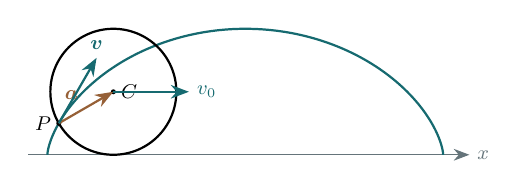
\begin{tikzpicture}[scale=.8,transform shape]
\draw[axis] (-.3,0)--(6.7,0) node[right] {$x$};\draw[traj] plot coordinates {(0.000000000,0.000000000) (0.000007088,0.000609173) (0.000056696,0.002435950) (0.000191292,0.005478105) (0.000453239,0.009731931) (0.000884748,0.015192247) (0.001527819,0.021852399) (0.002424200,0.029704274) (0.003615325,0.038738304) (0.005142271,0.048943484) (0.007045707,0.060307379) (0.009365842,0.072816145) (0.012142377,0.086454542) (0.015414459,0.101205954) (0.019220628,0.117052407) (0.023598776,0.133974596) (0.028586096,0.151951904) (0.034219042,0.170962427) (0.040533278,0.190983006) (0.047563640,0.211989246) (0.055344091,0.233955557) (0.063907679,0.256855175) (0.073286500,0.280660200) (0.083511656,0.305341630) (0.094613215,0.330869394) (0.106620183,0.357212390) (0.119560457,0.384338525) (0.133460802,0.412214748) (0.148346809,0.440807097) (0.164242870,0.470080736) (0.181172147,0.500000000) (0.199156543,0.530528437) (0.218216675,0.561628853) (0.238371849,0.593263357) (0.259640037,0.625393407) (0.282037856,0.657979857) (0.305580545,0.690983006) (0.330281951,0.724362644) (0.356154505,0.758078104) (0.383209216,0.792088309) (0.411455649,0.826351822) (0.440901918,0.860826899) (0.471554676,0.895471537) (0.503419106,0.930243526) (0.536498915,0.965100503) (0.570796327,1.000000000) (0.606312085,1.034899497) (0.643045447,1.069756474) (0.680994187,1.104528463) (0.720154598,1.139173101) (0.760521499,1.173648178) (0.802088236,1.207911691) (0.844846696,1.241921896) (0.888787311,1.275637356) (0.933899076,1.309016994) (0.980169556,1.342020143) (1.027584908,1.374606593) (1.076129890,1.406736643) (1.125787886,1.438371147) (1.176540924,1.469471563) (1.228369699,1.500000000) (1.281253591,1.529919264) (1.335170700,1.559192903) (1.390097863,1.587785252) (1.446010689,1.615661475) (1.502883584,1.642787610) (1.560689787,1.669130606) (1.619401397,1.694658370) (1.678989412,1.719339800) (1.739423761,1.743144825) (1.800673343,1.766044443) (1.862706063,1.788010754) (1.925488871,1.809016994) (1.988987804,1.829037573) (2.053168029,1.848048096) (2.117993878,1.866025404) (2.183428900,1.882947593) (2.249435901,1.898794046) (2.315976990,1.913545458) (2.383013625,1.927183855) (2.450506660,1.939692621) (2.518416394,1.951056516) (2.586702617,1.961261696) (2.655324663,1.970295726) (2.724241453,1.978147601) (2.793411551,1.984807753) (2.862793212,1.990268069) (2.932344435,1.994521895) (3.002023010,1.997564050) (3.071786572,1.999390827) (3.141592654,2.000000000) (3.211398735,1.999390827) (3.281162297,1.997564050) (3.350840872,1.994521895) (3.420392095,1.990268069) (3.489773756,1.984807753) (3.558943855,1.978147601) (3.627860644,1.970295726) (3.696482690,1.961261696) (3.764768913,1.951056516) (3.832678647,1.939692621) (3.900171682,1.927183855) (3.967208317,1.913545458) (4.033749406,1.898794046) (4.099756407,1.882947593) (4.165191429,1.866025404) (4.230017278,1.848048096) (4.294197503,1.829037573) (4.357696437,1.809016994) (4.420479245,1.788010754) (4.482511964,1.766044443) (4.543761546,1.743144825) (4.604195895,1.719339800) (4.663783910,1.694658370) (4.722495520,1.669130606) (4.780301723,1.642787610) (4.837174618,1.615661475) (4.893087444,1.587785252) (4.948014607,1.559192903) (5.001931716,1.529919264) (5.054815609,1.500000000) (5.106644383,1.469471563) (5.157397421,1.438371147) (5.207055418,1.406736643) (5.255600400,1.374606593) (5.303015751,1.342020143) (5.349286231,1.309016994) (5.394397996,1.275637356) (5.438338611,1.241921896) (5.481097071,1.207911691) (5.522663808,1.173648178) (5.563030709,1.139173101) (5.602191121,1.104528463) (5.640139861,1.069756474) (5.676873222,1.034899497) (5.712388980,1.000000000) (5.746686392,0.965100503) (5.779766201,0.930243526) (5.811630631,0.895471537) (5.842283389,0.860826899) (5.871729659,0.826351822) (5.899976091,0.792088309) (5.927030802,0.758078104) (5.952903357,0.724362644) (5.977604762,0.690983006) (6.001147452,0.657979857) (6.023545270,0.625393407) (6.044813459,0.593263357) (6.064968632,0.561628853) (6.084028764,0.530528437) (6.102013160,0.500000000) (6.118942437,0.470080736) (6.134838499,0.440807097) (6.149724505,0.412214748) (6.163624850,0.384338525) (6.176565124,0.357212390) (6.188572092,0.330869394) (6.199673652,0.305341630) (6.209898807,0.280660200) (6.219277628,0.256855175) (6.227841216,0.233955557) (6.235621667,0.211989246) (6.242652029,0.190983006) (6.248966265,0.170962427) (6.254599211,0.151951904) (6.259586532,0.133974596) (6.263964679,0.117052407) (6.267770848,0.101205954) (6.271042930,0.086454542) (6.273819465,0.072816145) (6.276139600,0.060307379) (6.278043036,0.048943484) (6.279569983,0.038738304) (6.280761108,0.029704274) (6.281657488,0.021852399) (6.282300560,0.015192247) (6.282732068,0.009731931) (6.282994015,0.005478105) (6.283128611,0.002435950) (6.283178219,0.000609173) (6.283185307,0.000000000)};\draw[thick] (1.0471975511965976,1) circle(1);\fill (1.0471975511965976,1) circle(.04) node[right] {$C$};\fill (0.18117214741215903,0.4999999999999999) circle(.04) node[left] {$P$};\draw[force] (0.18117214741215903,0.4999999999999999)--(1.0471975511965976,1) node[midway,above left] {$\boldsymbol a$};\draw[motion] (0.18117214741215903,0.4999999999999999)--(0.781172147412159,1.539230484541326) node[above] {$\boldsymbol v$};\draw[motion] (1.0471975511965976,1)--(2.2471975511965976,1) node[right] {$v_0$};
\end{tikzpicture}
\figcaption{解图综三.1A\quad 真实滚轮线与生成圆，横纵同尺度；加速度指向轮心}
\end{minipage}\end{center}
第（2）问，解图综三.1A取地面接地点为参数起点，$y$向上。设圆环转过$\theta$，纯滚动给环心平移$R\theta$，故
\[
x=R(\theta-\sin\theta),\qquad
y=R(1-\cos\theta).
\]
环心坐标为$(R\theta,R)$，轮上点相对环心的坐标为$(-R\sin\theta,-R\cos\theta)$，逐分量相加就是这组参数式。只要向前纯滚动，转角可以随时间非匀速增加，所有位置仍依次落在这条曲线上。轨迹的几何形状与$\theta$随时间变化的方式无关。为计算曲率，可选择环心匀速的方便运动：
\[
\begin{aligned}
\dot x&=v_0(1-\cos\theta),&
\dot y&=v_0\sin\theta,\\
\ddot x&=\frac{v_0^2}{R}\sin\theta,&
\ddot y&=\frac{v_0^2}{R}\cos\theta.
\end{aligned}
\]
对$0<\theta<2\pi$，
\[
v=2v_0\sin\frac\theta2,\qquad
|\dot x\ddot y-\dot y\ddot x|
=\frac{2v_0^3}{R}\sin^2\frac\theta2.
\]
速度平方化简用$(1-\cos\theta)^2+\sin^2\theta=2(1-\cos\theta)=4\sin^2(\theta/2)$。叉积中的三角项为$(1-\cos\theta)\cos\theta-\sin^2\theta=\cos\theta-1$，取绝对值得到上式。曲率只由轨迹的局部几何决定，分子、分母中所选生成速率的三次因子随后相消。因此正则点曲率半径为
\[
\boxed{\rho=
\frac{(\dot x^2+\dot y^2)^{3/2}}
{|\dot x\ddot y-\dot y\ddot x|}
=4R\sin\frac\theta2}.
\]
\begin{center}\begin{minipage}{.98\linewidth}\centering
\begin{tikzpicture}[scale=.8,transform shape]
\draw[axis] (-1,0)--(1.2,0) node[right] {$x$};\draw[axis] (0,0)--(0,3.1) node[above] {切线极限};\draw[traj] plot coordinates {(-0.661151273,2.426346325) (-0.637173821,2.369237475) (-0.613764646,2.312691696) (-0.590918091,2.256714643) (-0.568628439,2.201311914) (-0.546889920,2.146489049) (-0.525696707,2.092251530) (-0.505042920,2.038604781) (-0.484922624,1.985554167) (-0.465329832,1.933104992) (-0.446258502,1.881262502) (-0.427702542,1.830031880) (-0.409655808,1.779418250) (-0.392112104,1.729426673) (-0.375065184,1.680062148) (-0.358508754,1.631329612) (-0.342436469,1.583233937) (-0.326841936,1.535779934) (-0.311718716,1.488972347) (-0.297060319,1.442815857) (-0.282860213,1.397315081) (-0.269111817,1.352474567) (-0.255808506,1.308298801) (-0.242943610,1.264792199) (-0.230510417,1.221959112) (-0.218502169,1.179803824) (-0.206912067,1.138330549) (-0.195733270,1.097543436) (-0.184958897,1.057446563) (-0.174582025,1.018043939) (-0.164595691,0.979339505) (-0.154992895,0.941337131) (-0.145766596,0.904040618) (-0.136909717,0.867453694) (-0.128415144,0.831580020) (-0.120275727,0.796423181) (-0.112484279,0.761986694) (-0.105033581,0.728274003) (-0.097916376,0.695288478) (-0.091125376,0.663033417) (-0.084653262,0.631512048) (-0.078492679,0.600727521) (-0.072636245,0.570682915) (-0.067076544,0.541381235) (-0.061806134,0.512825411) (-0.056817540,0.485018297) (-0.052103263,0.457962676) (-0.047655773,0.431661252) (-0.043467515,0.406116655) (-0.039530908,0.381331441) (-0.035838347,0.357308087) (-0.032382199,0.334048996) (-0.029154811,0.311556494) (-0.026148506,0.289832829) (-0.023355585,0.268880175) (-0.020768326,0.248700626) (-0.018378989,0.229296201) (-0.016179812,0.210668840) (-0.014163015,0.192820405) (-0.012320801,0.175752682) (-0.010645354,0.159467377) (-0.009128840,0.143966119) (-0.007763413,0.129250458) (-0.006541207,0.115321865) (-0.005454347,0.102181733) (-0.004494940,0.089831377) (-0.003655083,0.078272030) (-0.002926859,0.067504850) (-0.002302342,0.057530913) (-0.001773593,0.048351216) (-0.001332667,0.039966678) (-0.000971606,0.032378136) (-0.000682448,0.025586350) (-0.000457221,0.019591998) (-0.000287948,0.014395681) (-0.000166646,0.009997917) (-0.000085327,0.006399147) (-0.000035998,0.003599730) (-0.000010666,0.001599947) (-0.000001333,0.000399997) (0.000000000,0.000000000) (0.000001333,0.000399997) (0.000010666,0.001599947) (0.000035998,0.003599730) (0.000085327,0.006399147) (0.000166646,0.009997917) (0.000287948,0.014395681) (0.000457221,0.019591998) (0.000682448,0.025586350) (0.000971606,0.032378136) (0.001332667,0.039966678) (0.001773593,0.048351216) (0.002302342,0.057530913) (0.002926859,0.067504850) (0.003655083,0.078272030) (0.004494940,0.089831377) (0.005454347,0.102181733) (0.006541207,0.115321865) (0.007763413,0.129250458) (0.009128840,0.143966119) (0.010645354,0.159467377) (0.012320801,0.175752682) (0.014163015,0.192820405) (0.016179812,0.210668840) (0.018378989,0.229296201) (0.020768326,0.248700626) (0.023355585,0.268880175) (0.026148506,0.289832829) (0.029154811,0.311556494) (0.032382199,0.334048996) (0.035838347,0.357308087) (0.039530908,0.381331441) (0.043467515,0.406116655) (0.047655773,0.431661252) (0.052103263,0.457962676) (0.056817540,0.485018297) (0.061806134,0.512825411) (0.067076544,0.541381235) (0.072636245,0.570682915) (0.078492679,0.600727521) (0.084653262,0.631512048) (0.091125376,0.663033417) (0.097916376,0.695288478) (0.105033581,0.728274003) (0.112484279,0.761986694) (0.120275727,0.796423181) (0.128415144,0.831580020) (0.136909717,0.867453694) (0.145766596,0.904040618) (0.154992895,0.941337131) (0.164595691,0.979339505) (0.174582025,1.018043939) (0.184958897,1.057446563) (0.195733270,1.097543436) (0.206912067,1.138330549) (0.218502169,1.179803824) (0.230510417,1.221959112) (0.242943610,1.264792199) (0.255808506,1.308298801) (0.269111817,1.352474567) (0.282860213,1.397315081) (0.297060319,1.442815857) (0.311718716,1.488972347) (0.326841936,1.535779934) (0.342436469,1.583233937) (0.358508754,1.631329612) (0.375065184,1.680062148) (0.392112104,1.729426673) (0.409655808,1.779418250) (0.427702542,1.830031880) (0.446258502,1.881262502) (0.465329832,1.933104992) (0.484922624,1.985554167) (0.505042920,2.038604781) (0.525696707,2.092251530) (0.546889920,2.146489049) (0.568628439,2.201311914) (0.590918091,2.256714643) (0.613764646,2.312691696) (0.637173821,2.369237475) (0.661151273,2.426346325)};\fill (0,0) circle(.04) node[below] {接地尖点};\node at (0,-.8) {$x\sim R\theta^3/6,\quad y\sim R\theta^2/2$};
\end{tikzpicture}
\figcaption{解图综三.1B\quad 真实尖点曲线，两坐标共同放大8倍}
\end{minipage}\end{center}
解图综三.1B放大最低接地位置。$\theta=0$时轨迹参数导数为零，是尖点，不是普通光滑点；曲率由两侧邻近的正则点取极限描述。邻近点满足
\[
x\simeq\frac R6\theta^3,\qquad
y\simeq\frac R2\theta^2,
\]
两侧切线都趋于竖直方向。更具体地，$\mathrm dx/\mathrm dy=(1-\cos\theta)/\sin\theta=\tan(\theta/2)\to0$，横向变化相对竖向变化更小。速度在尖点为零，切线却由邻近位移方向确定，图B的两侧分支都贴向同一竖直直线。由上面的正则点公式，
\[
\boxed{\rho_1=\lim_{\theta\to0^+}\rho=0}.
\]
曲率半径趋零描述的是邻近正则曲线的弯曲圆越来越小。与此同时，速度也趋零，比较二者的相对阶数才给法向加速度；这两个极限与尖点处的有限总加速度分别对应不同量。在所选匀速生成运动中，法向加速度为
$a_n=(v_0^2/R)\sin(\theta/2)$，也趋于零；尖点处有限的总加速度主要沿切线极限方向，切向与法向分量分别按速度方向分解。

最高点$\theta=\pi$是光滑点，速度水平、大小$2v_0$，加速度竖直向下，纯法向，故
\[
\boxed{\rho_2=\frac{(2v_0)^2}{v_0^2/R}=4R}.
\]
它与参数曲率式在$\theta=\pi$的值一致。
\begin{center}\begin{minipage}{.98\linewidth}\centering
\begin{tikzpicture}[scale=.8,transform shape]
\draw[axis] (-.3,0)--(6.7,0) node[right] {$x$};\draw[axis] (0,.4)--(0,-2.7) node[below] {$y$向下};\draw[traj] plot coordinates {(0.000000000,-0.000000000) (0.000007088,-0.000609173) (0.000056696,-0.002435950) (0.000191292,-0.005478105) (0.000453239,-0.009731931) (0.000884748,-0.015192247) (0.001527819,-0.021852399) (0.002424200,-0.029704274) (0.003615325,-0.038738304) (0.005142271,-0.048943484) (0.007045707,-0.060307379) (0.009365842,-0.072816145) (0.012142377,-0.086454542) (0.015414459,-0.101205954) (0.019220628,-0.117052407) (0.023598776,-0.133974596) (0.028586096,-0.151951904) (0.034219042,-0.170962427) (0.040533278,-0.190983006) (0.047563640,-0.211989246) (0.055344091,-0.233955557) (0.063907679,-0.256855175) (0.073286500,-0.280660200) (0.083511656,-0.305341630) (0.094613215,-0.330869394) (0.106620183,-0.357212390) (0.119560457,-0.384338525) (0.133460802,-0.412214748) (0.148346809,-0.440807097) (0.164242870,-0.470080736) (0.181172147,-0.500000000) (0.199156543,-0.530528437) (0.218216675,-0.561628853) (0.238371849,-0.593263357) (0.259640037,-0.625393407) (0.282037856,-0.657979857) (0.305580545,-0.690983006) (0.330281951,-0.724362644) (0.356154505,-0.758078104) (0.383209216,-0.792088309) (0.411455649,-0.826351822) (0.440901918,-0.860826899) (0.471554676,-0.895471537) (0.503419106,-0.930243526) (0.536498915,-0.965100503) (0.570796327,-1.000000000) (0.606312085,-1.034899497) (0.643045447,-1.069756474) (0.680994187,-1.104528463) (0.720154598,-1.139173101) (0.760521499,-1.173648178) (0.802088236,-1.207911691) (0.844846696,-1.241921896) (0.888787311,-1.275637356) (0.933899076,-1.309016994) (0.980169556,-1.342020143) (1.027584908,-1.374606593) (1.076129890,-1.406736643) (1.125787886,-1.438371147) (1.176540924,-1.469471563) (1.228369699,-1.500000000) (1.281253591,-1.529919264) (1.335170700,-1.559192903) (1.390097863,-1.587785252) (1.446010689,-1.615661475) (1.502883584,-1.642787610) (1.560689787,-1.669130606) (1.619401397,-1.694658370) (1.678989412,-1.719339800) (1.739423761,-1.743144825) (1.800673343,-1.766044443) (1.862706063,-1.788010754) (1.925488871,-1.809016994) (1.988987804,-1.829037573) (2.053168029,-1.848048096) (2.117993878,-1.866025404) (2.183428900,-1.882947593) (2.249435901,-1.898794046) (2.315976990,-1.913545458) (2.383013625,-1.927183855) (2.450506660,-1.939692621) (2.518416394,-1.951056516) (2.586702617,-1.961261696) (2.655324663,-1.970295726) (2.724241453,-1.978147601) (2.793411551,-1.984807753) (2.862793212,-1.990268069) (2.932344435,-1.994521895) (3.002023010,-1.997564050) (3.071786572,-1.999390827) (3.141592654,-2.000000000) (3.211398735,-1.999390827) (3.281162297,-1.997564050) (3.350840872,-1.994521895) (3.420392095,-1.990268069) (3.489773756,-1.984807753) (3.558943855,-1.978147601) (3.627860644,-1.970295726) (3.696482690,-1.961261696) (3.764768913,-1.951056516) (3.832678647,-1.939692621) (3.900171682,-1.927183855) (3.967208317,-1.913545458) (4.033749406,-1.898794046) (4.099756407,-1.882947593) (4.165191429,-1.866025404) (4.230017278,-1.848048096) (4.294197503,-1.829037573) (4.357696437,-1.809016994) (4.420479245,-1.788010754) (4.482511964,-1.766044443) (4.543761546,-1.743144825) (4.604195895,-1.719339800) (4.663783910,-1.694658370) (4.722495520,-1.669130606) (4.780301723,-1.642787610) (4.837174618,-1.615661475) (4.893087444,-1.587785252) (4.948014607,-1.559192903) (5.001931716,-1.529919264) (5.054815609,-1.500000000) (5.106644383,-1.469471563) (5.157397421,-1.438371147) (5.207055418,-1.406736643) (5.255600400,-1.374606593) (5.303015751,-1.342020143) (5.349286231,-1.309016994) (5.394397996,-1.275637356) (5.438338611,-1.241921896) (5.481097071,-1.207911691) (5.522663808,-1.173648178) (5.563030709,-1.139173101) (5.602191121,-1.104528463) (5.640139861,-1.069756474) (5.676873222,-1.034899497) (5.712388980,-1.000000000) (5.746686392,-0.965100503) (5.779766201,-0.930243526) (5.811630631,-0.895471537) (5.842283389,-0.860826899) (5.871729659,-0.826351822) (5.899976091,-0.792088309) (5.927030802,-0.758078104) (5.952903357,-0.724362644) (5.977604762,-0.690983006) (6.001147452,-0.657979857) (6.023545270,-0.625393407) (6.044813459,-0.593263357) (6.064968632,-0.561628853) (6.084028764,-0.530528437) (6.102013160,-0.500000000) (6.118942437,-0.470080736) (6.134838499,-0.440807097) (6.149724505,-0.412214748) (6.163624850,-0.384338525) (6.176565124,-0.357212390) (6.188572092,-0.330869394) (6.199673652,-0.305341630) (6.209898807,-0.280660200) (6.219277628,-0.256855175) (6.227841216,-0.233955557) (6.235621667,-0.211989246) (6.242652029,-0.190983006) (6.248966265,-0.170962427) (6.254599211,-0.151951904) (6.259586532,-0.133974596) (6.263964679,-0.117052407) (6.267770848,-0.101205954) (6.271042930,-0.086454542) (6.273819465,-0.072816145) (6.276139600,-0.060307379) (6.278043036,-0.048943484) (6.279569983,-0.038738304) (6.280761108,-0.029704274) (6.281657488,-0.021852399) (6.282300560,-0.015192247) (6.282732068,-0.009731931) (6.282994015,-0.005478105) (6.283128611,-0.002435950) (6.283178219,-0.000609173) (6.283185307,-0.000000000)};\fill (3.141592653589793,-2) circle(.05) node[below] {稳定最低点};\fill (3.141592653589793,2) circle(.05) node[above] {$O$};\draw[guide] (3.141592653589793,-2)--(3.141592653589793,2) node[midway,right] {$4R$};\draw[dashed,color=warm] plot coordinates {(1.583919284,-1.684243976) (1.633179540,-1.704684855) (1.682707953,-1.724467134) (1.732495720,-1.743587295) (1.782533990,-1.762041939) (1.832813866,-1.779827785) (1.883326411,-1.796941672) (1.934062644,-1.813380558) (1.985013546,-1.829141518) (2.036170059,-1.844221753) (2.087523089,-1.858618581) (2.139063506,-1.872329442) (2.190782148,-1.885351899) (2.242669820,-1.897683638) (2.294717299,-1.909322465) (2.346915330,-1.920266311) (2.399254636,-1.930513232) (2.451725911,-1.940061405) (2.504319827,-1.948909134) (2.557027034,-1.957054844) (2.609838163,-1.964497088) (2.662743824,-1.971234543) (2.715734613,-1.977266012) (2.768801109,-1.982590421) (2.821933878,-1.987206825) (2.875123474,-1.991114403) (2.928360442,-1.994312459) (2.981635317,-1.996800427) (3.034938628,-1.998577862) (3.088260900,-1.999644450) (3.141592654,-2.000000000) (3.194924407,-1.999644450) (3.248246679,-1.998577862) (3.301549990,-1.996800427) (3.354824866,-1.994312459) (3.408061833,-1.991114403) (3.461251429,-1.987206825) (3.514384198,-1.982590421) (3.567450694,-1.977266012) (3.620441483,-1.971234543) (3.673347144,-1.964497088) (3.726158273,-1.957054844) (3.778865480,-1.948909134) (3.831459396,-1.940061405) (3.883930671,-1.930513232) (3.936269977,-1.920266311) (3.988468009,-1.909322465) (4.040515487,-1.897683638) (4.092403159,-1.885351899) (4.144121801,-1.872329442) (4.195662218,-1.858618581) (4.247015248,-1.844221753) (4.298171761,-1.829141518) (4.349122663,-1.813380558) (4.399858896,-1.796941672) (4.450371441,-1.779827785) (4.500651317,-1.762041939) (4.550689587,-1.743587295) (4.600477354,-1.724467134) (4.650005767,-1.704684855) (4.699266023,-1.684243976)};
\end{tikzpicture}
\figcaption{解图综三.1C\quad 倒置凹轨道最低点的曲率圆半径4R，横纵同尺度}
\end{minipage}\end{center}
第（3）问，解图综三.1C改取$y$向下，凹轨道仍可用
$x=R(\theta-\sin\theta),y=R(1-\cos\theta)$表示。稳定最低点在$\theta=\pi$，其曲率半径是$4R$，它位于一拱的光滑中部。

两种朝向的最高、最低位置随倒置互换，第三问用的光滑最低点对应第二问的光滑最高点，几何曲率半径保持相同。取该点附近的短轨道，用其曲率圆近似时，误差从更高阶位移开始，线性的切向恢复力由这个半径决定。

因为已知周期与振幅无关，可以取任意小振幅。在最低点附近，轨道等同于半径$4R$的曲率圆，等效小角单摆长$4R$：
\[
\boxed{T=2\pi\sqrt{\frac{4R}{g}}
=4\pi\sqrt{\frac Rg}}.
\]
这个推理用到了题给等时性；对一般光滑曲线，用最低点曲率只能求小振幅周期，有限振幅还由轨道整段的势能关系决定。
\begin{center}\begin{minipage}{.98\linewidth}\centering
\begin{tikzpicture}[scale=.8,transform shape]
\draw[axis] (0,0)--(10.7,0) node[right] {$s/R$};
\draw[axis] (0,0)--(0,3.2) node[above] {$\Delta h/R$};\foreach \y/\lab in {0/0,1.3/1,2.6/2}{\draw[thin] (0,\y)--(-.08,\y) node[left] {$\lab$};}
\node[above] at (5,3.5) {有向弧长坐标下，高度精确为二次函数};
\draw[traj] plot coordinates {(0.250000000,2.346500000) (0.329166667,2.268935139) (0.408333333,2.192673889) (0.487500000,2.117716250) (0.566666667,2.044062222) (0.645833333,1.971711806) (0.725000000,1.900665000) (0.804166667,1.830921806) (0.883333333,1.762482222) (0.962500000,1.695346250) (1.041666667,1.629513889) (1.120833333,1.564985139) (1.200000000,1.501760000) (1.279166667,1.439838472) (1.358333333,1.379220556) (1.437500000,1.319906250) (1.516666667,1.261895556) (1.595833333,1.205188472) (1.675000000,1.149785000) (1.754166667,1.095685139) (1.833333333,1.042888889) (1.912500000,0.991396250) (1.991666667,0.941207222) (2.070833333,0.892321806) (2.150000000,0.844740000) (2.229166667,0.798461806) (2.308333333,0.753487222) (2.387500000,0.709816250) (2.466666667,0.667448889) (2.545833333,0.626385139) (2.625000000,0.586625000) (2.704166667,0.548168472) (2.783333333,0.511015556) (2.862500000,0.475166250) (2.941666667,0.440620556) (3.020833333,0.407378472) (3.100000000,0.375440000) (3.179166667,0.344805139) (3.258333333,0.315473889) (3.337500000,0.287446250) (3.416666667,0.260722222) (3.495833333,0.235301806) (3.575000000,0.211185000) (3.654166667,0.188371806) (3.733333333,0.166862222) (3.812500000,0.146656250) (3.891666667,0.127753889) (3.970833333,0.110155139) (4.050000000,0.093860000) (4.129166667,0.078868472) (4.208333333,0.065180556) (4.287500000,0.052796250) (4.366666667,0.041715556) (4.445833333,0.031938472) (4.525000000,0.023465000) (4.604166667,0.016295139) (4.683333333,0.010428889) (4.762500000,0.005866250) (4.841666667,0.002607222) (4.920833333,0.000651806) (5.000000000,0.000000000) (5.079166667,0.000651806) (5.158333333,0.002607222) (5.237500000,0.005866250) (5.316666667,0.010428889) (5.395833333,0.016295139) (5.475000000,0.023465000) (5.554166667,0.031938472) (5.633333333,0.041715556) (5.712500000,0.052796250) (5.791666667,0.065180556) (5.870833333,0.078868472) (5.950000000,0.093860000) (6.029166667,0.110155139) (6.108333333,0.127753889) (6.187500000,0.146656250) (6.266666667,0.166862222) (6.345833333,0.188371806) (6.425000000,0.211185000) (6.504166667,0.235301806) (6.583333333,0.260722222) (6.662500000,0.287446250) (6.741666667,0.315473889) (6.820833333,0.344805139) (6.900000000,0.375440000) (6.979166667,0.407378472) (7.058333333,0.440620556) (7.137500000,0.475166250) (7.216666667,0.511015556) (7.295833333,0.548168472) (7.375000000,0.586625000) (7.454166667,0.626385139) (7.533333333,0.667448889) (7.612500000,0.709816250) (7.691666667,0.753487222) (7.770833333,0.798461806) (7.850000000,0.844740000) (7.929166667,0.892321806) (8.008333333,0.941207222) (8.087500000,0.991396250) (8.166666667,1.042888889) (8.245833333,1.095685139) (8.325000000,1.149785000) (8.404166667,1.205188472) (8.483333333,1.261895556) (8.562500000,1.319906250) (8.641666667,1.379220556) (8.720833333,1.439838472) (8.800000000,1.501760000) (8.879166667,1.564985139) (8.958333333,1.629513889) (9.037500000,1.695346250) (9.116666667,1.762482222) (9.195833333,1.830921806) (9.275000000,1.900665000) (9.354166667,1.971711806) (9.433333333,2.044062222) (9.512500000,2.117716250) (9.591666667,2.192673889) (9.670833333,2.268935139) (9.750000000,2.346500000)};
\node[below] at (0,-.12) {$-4$};
\node[below] at (5,-.12) {$0$};
\node[below] at (10,-.12) {$4$};
\end{tikzpicture}
\figcaption{解图综三.1D\quad 有向弧长坐标下，高度精确为二次函数}
\end{minipage}\end{center}
解图综三.1D把最低点量起的有向弧长$s$与竖直上升高度相联系。沿一拱$0<\theta<2\pi$，
\[
\frac{ds}{d\theta}=2R\sin\frac\theta2,\qquad
s(\pi)=0,
\]
积分下限选在$\theta=\pi$，有$s=\int_\pi^\theta2R\sin(\eta/2)\mathrm d\eta=-4R\cos(\theta/2)$，使右侧位置为正、左侧位置为负。这个符号约定和$\mathrm ds/\mathrm d\theta>0$一致，所以
\[
s=-4R\cos\frac\theta2.
\]
小球相对最低点的竖直上升高度为
\[
\Delta h=2R-y=2R\cos^2\frac\theta2
=\frac{s^2}{8R}.
\]
以弧长作广义坐标，沿轨道的速率就是$|\dot s|$，动能为$m\dot s^2/2$，势能为$mg\Delta h$。沿弧长的重力分量为势能的负导数，质量在运动方程两端相消，切向运动方程或能量的弧长导数给
\[
m\ddot s=-mg\frac{d\Delta h}{ds}
=-\frac{mg}{4R}s,
\qquad
\ddot s+\frac g{4R}s=0.
\]
它对一拱内的有限振幅也是严格简谐方程，再次给全周期$4\pi\sqrt{R/g}$。一侧释放至最低点为四分之一周期，完整往返包含四段这样的运动。
从静止释放时$s(0)=s_0,\dot s(0)=0$，因此$s=s_0\cos[\sqrt{g/(4R)}\,t]$；质量和$s_0$只影响能量及运动幅度，方程中的频率保持相同。振幅限定在$|s_0|<4R$，对应一拱内的光滑释放点，运动在两个等高转向点之间往返。到最低点时速度最大，再爬升到另一侧转向，接着按相反次序返回，完整过程构成上式的一个周期。



\Needspace{8\baselineskip}

\pdfbookmark[3]{关键洞察}{q1-h5}

\subsection*{关键洞察}

接地尖点的参数速度为零、两侧切线极限竖直，曲率半径以极限零描述。倒置摆线的稳定最低点在拱中部，是曲率半径$4R$的光滑点。两种最低位置各属于不同朝向的图。总加速度保持恒模时，其切向、法向分量仍随位置变化；最低点曲率先给小振幅周期，弧长二次势能使本题全振幅都满足同一周期。

\Needspace{8\baselineskip}

\pdfbookmark[3]{易错点}{q1-h6}

\subsection*{易错点}

速度方向或大小改变时，加速度矢量相应变化，其模还需单独计算。接地尖点用参数展开确定切线方向，正则点曲率先算再取极限；一般点的法向加速度与总加速度分别计算。等时摆的最低点使用倒置图中光滑位置的曲率。从一侧静止释放到最低点经历四分之一周期，完整往返为一个周期，写结果时同时说明对应过程。

\Needspace{8\baselineskip}

\pdfbookmark[3]{课堂讲解建议}{q1-h7}

\subsection*{课堂讲解建议}

在图A先要求学生画指向轮心的加速度，再平移到地面系，说明两系加速度相同的条件。对尖点让学生把$x,y$分别展开到三次、二次项，算$\mathrm dx/\mathrm dy$的极限，再看图B的真实曲线，判断瞬心、切线和法向各描述什么。

讲第三问时换到图C重新指定向下纵轴，并指出稳定最低点的曲率圆心在其上方。先用题给等时性取小振幅，随后在图D积分弧长，写高度二次式和切向简谐方程。让学生依次说出从一侧到最低点、到另一侧及返回的时间，使几何方向、势能和周期在同一图像中对应。

\Needspace{8\baselineskip}

\pdfbookmark[3]{变式训练}{q1-h8}

\subsection*{变式训练}

\begin{enumerate}
\Needspace{20\baselineskip}
\item 在上方滚轮线$\theta=\pi/3$处，求曲率、速率与切向、法向加速度。
\textbf{解：}变图综三.1V1有$\rho=4R\sin(\pi/6)=2R$，$v=2v_0\sin(\pi/6)=v_0$。法向分量$a_n=v^2/\rho=v_0^2/(2R)$，总加速度模为$v_0^2/R$。切向分量由$\dot v=(v_0^2/R)\cos(\theta/2)$给$a_t=\sqrt3v_0^2/(2R)$，两者平方和恰为总加速度平方。加速度指向轮心，轨迹法线则由瞬时速度方向决定，两条方向在一般点不同。
\begin{center}\begin{minipage}{.98\linewidth}\centering
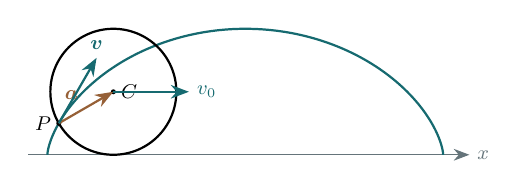
\begin{tikzpicture}[scale=.8,transform shape]
\draw[axis] (-.3,0)--(6.7,0) node[right] {$x$};\draw[traj] plot coordinates {(0.000000000,0.000000000) (0.000007088,0.000609173) (0.000056696,0.002435950) (0.000191292,0.005478105) (0.000453239,0.009731931) (0.000884748,0.015192247) (0.001527819,0.021852399) (0.002424200,0.029704274) (0.003615325,0.038738304) (0.005142271,0.048943484) (0.007045707,0.060307379) (0.009365842,0.072816145) (0.012142377,0.086454542) (0.015414459,0.101205954) (0.019220628,0.117052407) (0.023598776,0.133974596) (0.028586096,0.151951904) (0.034219042,0.170962427) (0.040533278,0.190983006) (0.047563640,0.211989246) (0.055344091,0.233955557) (0.063907679,0.256855175) (0.073286500,0.280660200) (0.083511656,0.305341630) (0.094613215,0.330869394) (0.106620183,0.357212390) (0.119560457,0.384338525) (0.133460802,0.412214748) (0.148346809,0.440807097) (0.164242870,0.470080736) (0.181172147,0.500000000) (0.199156543,0.530528437) (0.218216675,0.561628853) (0.238371849,0.593263357) (0.259640037,0.625393407) (0.282037856,0.657979857) (0.305580545,0.690983006) (0.330281951,0.724362644) (0.356154505,0.758078104) (0.383209216,0.792088309) (0.411455649,0.826351822) (0.440901918,0.860826899) (0.471554676,0.895471537) (0.503419106,0.930243526) (0.536498915,0.965100503) (0.570796327,1.000000000) (0.606312085,1.034899497) (0.643045447,1.069756474) (0.680994187,1.104528463) (0.720154598,1.139173101) (0.760521499,1.173648178) (0.802088236,1.207911691) (0.844846696,1.241921896) (0.888787311,1.275637356) (0.933899076,1.309016994) (0.980169556,1.342020143) (1.027584908,1.374606593) (1.076129890,1.406736643) (1.125787886,1.438371147) (1.176540924,1.469471563) (1.228369699,1.500000000) (1.281253591,1.529919264) (1.335170700,1.559192903) (1.390097863,1.587785252) (1.446010689,1.615661475) (1.502883584,1.642787610) (1.560689787,1.669130606) (1.619401397,1.694658370) (1.678989412,1.719339800) (1.739423761,1.743144825) (1.800673343,1.766044443) (1.862706063,1.788010754) (1.925488871,1.809016994) (1.988987804,1.829037573) (2.053168029,1.848048096) (2.117993878,1.866025404) (2.183428900,1.882947593) (2.249435901,1.898794046) (2.315976990,1.913545458) (2.383013625,1.927183855) (2.450506660,1.939692621) (2.518416394,1.951056516) (2.586702617,1.961261696) (2.655324663,1.970295726) (2.724241453,1.978147601) (2.793411551,1.984807753) (2.862793212,1.990268069) (2.932344435,1.994521895) (3.002023010,1.997564050) (3.071786572,1.999390827) (3.141592654,2.000000000) (3.211398735,1.999390827) (3.281162297,1.997564050) (3.350840872,1.994521895) (3.420392095,1.990268069) (3.489773756,1.984807753) (3.558943855,1.978147601) (3.627860644,1.970295726) (3.696482690,1.961261696) (3.764768913,1.951056516) (3.832678647,1.939692621) (3.900171682,1.927183855) (3.967208317,1.913545458) (4.033749406,1.898794046) (4.099756407,1.882947593) (4.165191429,1.866025404) (4.230017278,1.848048096) (4.294197503,1.829037573) (4.357696437,1.809016994) (4.420479245,1.788010754) (4.482511964,1.766044443) (4.543761546,1.743144825) (4.604195895,1.719339800) (4.663783910,1.694658370) (4.722495520,1.669130606) (4.780301723,1.642787610) (4.837174618,1.615661475) (4.893087444,1.587785252) (4.948014607,1.559192903) (5.001931716,1.529919264) (5.054815609,1.500000000) (5.106644383,1.469471563) (5.157397421,1.438371147) (5.207055418,1.406736643) (5.255600400,1.374606593) (5.303015751,1.342020143) (5.349286231,1.309016994) (5.394397996,1.275637356) (5.438338611,1.241921896) (5.481097071,1.207911691) (5.522663808,1.173648178) (5.563030709,1.139173101) (5.602191121,1.104528463) (5.640139861,1.069756474) (5.676873222,1.034899497) (5.712388980,1.000000000) (5.746686392,0.965100503) (5.779766201,0.930243526) (5.811630631,0.895471537) (5.842283389,0.860826899) (5.871729659,0.826351822) (5.899976091,0.792088309) (5.927030802,0.758078104) (5.952903357,0.724362644) (5.977604762,0.690983006) (6.001147452,0.657979857) (6.023545270,0.625393407) (6.044813459,0.593263357) (6.064968632,0.561628853) (6.084028764,0.530528437) (6.102013160,0.500000000) (6.118942437,0.470080736) (6.134838499,0.440807097) (6.149724505,0.412214748) (6.163624850,0.384338525) (6.176565124,0.357212390) (6.188572092,0.330869394) (6.199673652,0.305341630) (6.209898807,0.280660200) (6.219277628,0.256855175) (6.227841216,0.233955557) (6.235621667,0.211989246) (6.242652029,0.190983006) (6.248966265,0.170962427) (6.254599211,0.151951904) (6.259586532,0.133974596) (6.263964679,0.117052407) (6.267770848,0.101205954) (6.271042930,0.086454542) (6.273819465,0.072816145) (6.276139600,0.060307379) (6.278043036,0.048943484) (6.279569983,0.038738304) (6.280761108,0.029704274) (6.281657488,0.021852399) (6.282300560,0.015192247) (6.282732068,0.009731931) (6.282994015,0.005478105) (6.283128611,0.002435950) (6.283178219,0.000609173) (6.283185307,0.000000000)};\draw[thick] (1.0471975511965976,1) circle(1);\fill (1.0471975511965976,1) circle(.04) node[right] {$C$};\fill (0.18117214741215903,0.4999999999999999) circle(.04) node[left] {$P$};\draw[force] (0.18117214741215903,0.4999999999999999)--(1.0471975511965976,1) node[midway,above left] {$\boldsymbol a$};\draw[motion] (0.18117214741215903,0.4999999999999999)--(0.781172147412159,1.539230484541326) node[above] {$\boldsymbol v$};\draw[motion] (1.0471975511965976,1)--(2.2471975511965976,1) node[right] {$v_0$};
\end{tikzpicture}
\figcaption{变图综三.1V1\quad 真实滚轮线与生成圆，横纵同尺度；加速度指向轮心}
\end{minipage}\end{center}

\Needspace{20\baselineskip}
\item 把生成圆半径变成$4R$，分别讨论同位置角曲率、等时摆周期，以及固定环心速率时的加速度。
\textbf{解：}变图综三.1V2参数$x,y$都正比于生成半径，故同一$\theta$的曲率半径也乘4。周期$4\pi\sqrt{R/g}$随半径平方根变化，变为2倍。固定$v_0$时$\omega=v_0/R$降为四分之一，$\omega^2R=v_0^2/R$降为四分之一。几何长度、重力振动时间及匀速生成运动的加速度各按自己的关系缩放。
\begin{center}\begin{minipage}{.98\linewidth}\centering
\begin{tikzpicture}[scale=.8,transform shape]
\node[draw] at (0,1) {$R\to4R$};\node[draw] at (4,2) {$\rho\to4\rho$};\node[draw] at (4,1) {$T\to2T$};\node[draw] at (4,0) {$v_0$固定：$a\to a/4$};\draw[axis] (1,1)--(2,2);\draw[axis] (1,1)--(2,1);\draw[axis] (1,1)--(2,0);
\end{tikzpicture}
\figcaption{变图综三.1V2\quad 几何、重力周期与固定平移速率的加速度分别缩放}
\end{minipage}\end{center}

\Needspace{20\baselineskip}
\item 小球从弧长$s_0$处静止释放，求到最低点、到另一侧同高点及返回的时间。
\textbf{解：}变图综三.1V3令$\Omega_0=\sqrt{g/(4R)}$，零初速给$s=s_0\cos\Omega_0t$。第一次到最低点$s=0$时相位为$\pi/2$，时间$\pi\sqrt{R/g}$；到另一侧$s=-s_0$时相位为$\pi$，时间$2\pi\sqrt{R/g}$；回到初始位置且速度再次为零时相位为$2\pi$，时间$4\pi\sqrt{R/g}$。只要$|s_0|<4R$，这些时间都与振幅无关。
\begin{center}\begin{minipage}{.98\linewidth}\centering
\begin{tikzpicture}[scale=.8,transform shape]
\draw[axis] (0,0)--(10.7,0) node[right] {$\Omega_0t$};
\draw[axis] (0,0)--(0,3.2) node[above] {$s/s_0$};\foreach \y/\lab in {0.13/-1,2.73/1}{\draw[thin] (0,\y)--(-.08,\y) node[left] {$\lab$};}
\node[above] at (5,3.5) {零点、另一侧同高点与完整返回分别为四分之一、半个、一个周期};
\draw[traj] plot coordinates {(0.000000000,2.730000000) (0.062500000,2.728997747) (0.125000000,2.725992534) (0.187500000,2.720988994) (0.250000000,2.713994843) (0.312500000,2.705020865) (0.375000000,2.694080897) (0.437500000,2.681191807) (0.500000000,2.666373471) (0.562500000,2.649648737) (0.625000000,2.631043392) (0.687500000,2.610586126) (0.750000000,2.588308481) (0.812500000,2.564244809) (0.875000000,2.538432214) (0.937500000,2.510910496) (1.000000000,2.481722093) (1.062500000,2.450912010) (1.125000000,2.418527755) (1.187500000,2.384619262) (1.250000000,2.349238816) (1.312500000,2.312440969) (1.375000000,2.274282463) (1.437500000,2.234822134) (1.500000000,2.194120828) (1.562500000,2.152241303) (1.625000000,2.109248134) (1.687500000,2.065207614) (1.750000000,2.020187650) (1.812500000,1.974257659) (1.875000000,1.927488462) (1.937500000,1.879952174) (2.000000000,1.831722093) (2.062500000,1.782872585) (2.125000000,1.733478973) (2.187500000,1.683617419) (2.250000000,1.633364805) (2.312500000,1.582798617) (2.375000000,1.531996824) (2.437500000,1.481037760) (2.500000000,1.430000000) (2.562500000,1.378962240) (2.625000000,1.328003176) (2.687500000,1.277201383) (2.750000000,1.226635195) (2.812500000,1.176382581) (2.875000000,1.126521027) (2.937500000,1.077127415) (3.000000000,1.028277907) (3.062500000,0.980047826) (3.125000000,0.932511538) (3.187500000,0.885742341) (3.250000000,0.839812350) (3.312500000,0.794792386) (3.375000000,0.750751866) (3.437500000,0.707758697) (3.500000000,0.665879172) (3.562500000,0.625177866) (3.625000000,0.585717537) (3.687500000,0.547559031) (3.750000000,0.510761184) (3.812500000,0.475380738) (3.875000000,0.441472245) (3.937500000,0.409087990) (4.000000000,0.378277907) (4.062500000,0.349089504) (4.125000000,0.321567786) (4.187500000,0.295755191) (4.250000000,0.271691519) (4.312500000,0.249413874) (4.375000000,0.228956608) (4.437500000,0.210351263) (4.500000000,0.193626529) (4.562500000,0.178808193) (4.625000000,0.165919103) (4.687500000,0.154979135) (4.750000000,0.146005157) (4.812500000,0.139011006) (4.875000000,0.134007466) (4.937500000,0.131002253) (5.000000000,0.130000000) (5.062500000,0.131002253) (5.125000000,0.134007466) (5.187500000,0.139011006) (5.250000000,0.146005157) (5.312500000,0.154979135) (5.375000000,0.165919103) (5.437500000,0.178808193) (5.500000000,0.193626529) (5.562500000,0.210351263) (5.625000000,0.228956608) (5.687500000,0.249413874) (5.750000000,0.271691519) (5.812500000,0.295755191) (5.875000000,0.321567786) (5.937500000,0.349089504) (6.000000000,0.378277907) (6.062500000,0.409087990) (6.125000000,0.441472245) (6.187500000,0.475380738) (6.250000000,0.510761184) (6.312500000,0.547559031) (6.375000000,0.585717537) (6.437500000,0.625177866) (6.500000000,0.665879172) (6.562500000,0.707758697) (6.625000000,0.750751866) (6.687500000,0.794792386) (6.750000000,0.839812350) (6.812500000,0.885742341) (6.875000000,0.932511538) (6.937500000,0.980047826) (7.000000000,1.028277907) (7.062500000,1.077127415) (7.125000000,1.126521027) (7.187500000,1.176382581) (7.250000000,1.226635195) (7.312500000,1.277201383) (7.375000000,1.328003176) (7.437500000,1.378962240) (7.500000000,1.430000000) (7.562500000,1.481037760) (7.625000000,1.531996824) (7.687500000,1.582798617) (7.750000000,1.633364805) (7.812500000,1.683617419) (7.875000000,1.733478973) (7.937500000,1.782872585) (8.000000000,1.831722093) (8.062500000,1.879952174) (8.125000000,1.927488462) (8.187500000,1.974257659) (8.250000000,2.020187650) (8.312500000,2.065207614) (8.375000000,2.109248134) (8.437500000,2.152241303) (8.500000000,2.194120828) (8.562500000,2.234822134) (8.625000000,2.274282463) (8.687500000,2.312440969) (8.750000000,2.349238816) (8.812500000,2.384619262) (8.875000000,2.418527755) (8.937500000,2.450912010) (9.000000000,2.481722093) (9.062500000,2.510910496) (9.125000000,2.538432214) (9.187500000,2.564244809) (9.250000000,2.588308481) (9.312500000,2.610586126) (9.375000000,2.631043392) (9.437500000,2.649648737) (9.500000000,2.666373471) (9.562500000,2.681191807) (9.625000000,2.694080897) (9.687500000,2.705020865) (9.750000000,2.713994843) (9.812500000,2.720988994) (9.875000000,2.725992534) (9.937500000,2.728997747) (10.000000000,2.730000000)};
\node[below] at (0,-.12) {$0$};
\node[below] at (2.5,-.12) {$\pi/2$};
\node[below] at (5,-.12) {$\pi$};
\node[below] at (10,-.12) {$2\pi$};
\draw[dotted] (0,1.43)--(10,1.43);\node[left] at (0,1.43) {$0$};
\end{tikzpicture}
\figcaption{变图综三.1V3\quad 零点、另一侧同高点与完整返回分别为四分之一、半个、一个周期}
\end{minipage}\end{center}

\Needspace{20\baselineskip}
\item 改用半径$4R$的圆弧代替凹摆线，比较小振幅与有限振幅的周期。
\textbf{解：}变图综三.1V4圆弧用弧长$s$表示高度为$h=4R[1-\cos(s/(4R))]=s^2/(8R)-s^4/(1536R^3)+\cdots$。二次项与摆线相同，故无限小振幅周期相同；四次及更高项使恢复力偏离严格线性。圆弧摆最大角度为$\psi_0$时，能量积分展开给$T=4\pi\sqrt{R/g}[1+\psi_0^2/16+O(\psi_0^4)]$。摆线的高度二次式对整拱精确成立，圆弧仅在小振幅近似如此。
\begin{center}\begin{minipage}{.98\linewidth}\centering
\begin{tikzpicture}[scale=.8,transform shape]
\draw[axis] (0,0)--(10.7,0) node[right] {$s/R$};
\draw[axis] (0,0)--(0,3.2) node[above] {$\Delta h/R$};\foreach \y/\lab in {0/0,1.3/1,2.6/2}{\draw[thin] (0,\y)--(-.08,\y) node[left] {$\lab$};}
\node[above] at (5,3.5) {实线摆线，虚线半径$4R$圆弧；二次项相同，高阶项不同};
\draw[traj] plot coordinates {(0.250000000,2.346500000) (0.329166667,2.268935139) (0.408333333,2.192673889) (0.487500000,2.117716250) (0.566666667,2.044062222) (0.645833333,1.971711806) (0.725000000,1.900665000) (0.804166667,1.830921806) (0.883333333,1.762482222) (0.962500000,1.695346250) (1.041666667,1.629513889) (1.120833333,1.564985139) (1.200000000,1.501760000) (1.279166667,1.439838472) (1.358333333,1.379220556) (1.437500000,1.319906250) (1.516666667,1.261895556) (1.595833333,1.205188472) (1.675000000,1.149785000) (1.754166667,1.095685139) (1.833333333,1.042888889) (1.912500000,0.991396250) (1.991666667,0.941207222) (2.070833333,0.892321806) (2.150000000,0.844740000) (2.229166667,0.798461806) (2.308333333,0.753487222) (2.387500000,0.709816250) (2.466666667,0.667448889) (2.545833333,0.626385139) (2.625000000,0.586625000) (2.704166667,0.548168472) (2.783333333,0.511015556) (2.862500000,0.475166250) (2.941666667,0.440620556) (3.020833333,0.407378472) (3.100000000,0.375440000) (3.179166667,0.344805139) (3.258333333,0.315473889) (3.337500000,0.287446250) (3.416666667,0.260722222) (3.495833333,0.235301806) (3.575000000,0.211185000) (3.654166667,0.188371806) (3.733333333,0.166862222) (3.812500000,0.146656250) (3.891666667,0.127753889) (3.970833333,0.110155139) (4.050000000,0.093860000) (4.129166667,0.078868472) (4.208333333,0.065180556) (4.287500000,0.052796250) (4.366666667,0.041715556) (4.445833333,0.031938472) (4.525000000,0.023465000) (4.604166667,0.016295139) (4.683333333,0.010428889) (4.762500000,0.005866250) (4.841666667,0.002607222) (4.920833333,0.000651806) (5.000000000,0.000000000) (5.079166667,0.000651806) (5.158333333,0.002607222) (5.237500000,0.005866250) (5.316666667,0.010428889) (5.395833333,0.016295139) (5.475000000,0.023465000) (5.554166667,0.031938472) (5.633333333,0.041715556) (5.712500000,0.052796250) (5.791666667,0.065180556) (5.870833333,0.078868472) (5.950000000,0.093860000) (6.029166667,0.110155139) (6.108333333,0.127753889) (6.187500000,0.146656250) (6.266666667,0.166862222) (6.345833333,0.188371806) (6.425000000,0.211185000) (6.504166667,0.235301806) (6.583333333,0.260722222) (6.662500000,0.287446250) (6.741666667,0.315473889) (6.820833333,0.344805139) (6.900000000,0.375440000) (6.979166667,0.407378472) (7.058333333,0.440620556) (7.137500000,0.475166250) (7.216666667,0.511015556) (7.295833333,0.548168472) (7.375000000,0.586625000) (7.454166667,0.626385139) (7.533333333,0.667448889) (7.612500000,0.709816250) (7.691666667,0.753487222) (7.770833333,0.798461806) (7.850000000,0.844740000) (7.929166667,0.892321806) (8.008333333,0.941207222) (8.087500000,0.991396250) (8.166666667,1.042888889) (8.245833333,1.095685139) (8.325000000,1.149785000) (8.404166667,1.205188472) (8.483333333,1.261895556) (8.562500000,1.319906250) (8.641666667,1.379220556) (8.720833333,1.439838472) (8.800000000,1.501760000) (8.879166667,1.564985139) (8.958333333,1.629513889) (9.037500000,1.695346250) (9.116666667,1.762482222) (9.195833333,1.830921806) (9.275000000,1.900665000) (9.354166667,1.971711806) (9.433333333,2.044062222) (9.512500000,2.117716250) (9.591666667,2.192673889) (9.670833333,2.268935139) (9.750000000,2.346500000)};
\draw[dashed,thick,color=warm] plot coordinates {(0.250000000,2.175247935) (0.329166667,2.108658659) (0.408333333,2.042844350) (0.487500000,1.977821505) (0.566666667,1.913606426) (0.645833333,1.850215210) (0.725000000,1.787663749) (0.804166667,1.725967724) (0.883333333,1.665142602) (0.962500000,1.605203630) (1.041666667,1.546165834) (1.120833333,1.488044015) (1.200000000,1.430852744) (1.279166667,1.374606357) (1.358333333,1.319318955) (1.437500000,1.265004398) (1.516666667,1.211676302) (1.595833333,1.159348036) (1.675000000,1.108032717) (1.754166667,1.057743211) (1.833333333,1.008492123) (1.912500000,0.960291802) (1.991666667,0.913154329) (2.070833333,0.867091522) (2.150000000,0.822114929) (2.229166667,0.778235824) (2.308333333,0.735465208) (2.387500000,0.693813803) (2.466666667,0.653292050) (2.545833333,0.613910107) (2.625000000,0.575677848) (2.704166667,0.538604856) (2.783333333,0.502700426) (2.862500000,0.467973558) (2.941666667,0.434432958) (3.020833333,0.402087034) (3.100000000,0.370943895) (3.179166667,0.341011348) (3.258333333,0.312296898) (3.337500000,0.284807742) (3.416666667,0.258550771) (3.495833333,0.233532569) (3.575000000,0.209759406) (3.654166667,0.187237243) (3.733333333,0.165971725) (3.812500000,0.145968184) (3.891666667,0.127231634) (3.970833333,0.109766773) (4.050000000,0.093577977) (4.129166667,0.078669307) (4.208333333,0.065044499) (4.287500000,0.052706969) (4.366666667,0.041659810) (4.445833333,0.031905791) (4.525000000,0.023447358) (4.604166667,0.016286630) (4.683333333,0.010425403) (4.762500000,0.005865147) (4.841666667,0.002607004) (4.920833333,0.000651792) (5.000000000,0.000000000) (5.079166667,0.000651792) (5.158333333,0.002607004) (5.237500000,0.005865147) (5.316666667,0.010425403) (5.395833333,0.016286630) (5.475000000,0.023447358) (5.554166667,0.031905791) (5.633333333,0.041659810) (5.712500000,0.052706969) (5.791666667,0.065044499) (5.870833333,0.078669307) (5.950000000,0.093577977) (6.029166667,0.109766773) (6.108333333,0.127231634) (6.187500000,0.145968184) (6.266666667,0.165971725) (6.345833333,0.187237243) (6.425000000,0.209759406) (6.504166667,0.233532569) (6.583333333,0.258550771) (6.662500000,0.284807742) (6.741666667,0.312296898) (6.820833333,0.341011348) (6.900000000,0.370943895) (6.979166667,0.402087034) (7.058333333,0.434432958) (7.137500000,0.467973558) (7.216666667,0.502700426) (7.295833333,0.538604856) (7.375000000,0.575677848) (7.454166667,0.613910107) (7.533333333,0.653292050) (7.612500000,0.693813803) (7.691666667,0.735465208) (7.770833333,0.778235824) (7.850000000,0.822114929) (7.929166667,0.867091522) (8.008333333,0.913154329) (8.087500000,0.960291802) (8.166666667,1.008492123) (8.245833333,1.057743211) (8.325000000,1.108032717) (8.404166667,1.159348036) (8.483333333,1.211676302) (8.562500000,1.265004398) (8.641666667,1.319318955) (8.720833333,1.374606357) (8.800000000,1.430852744) (8.879166667,1.488044015) (8.958333333,1.546165834) (9.037500000,1.605203630) (9.116666667,1.665142602) (9.195833333,1.725967724) (9.275000000,1.787663749) (9.354166667,1.850215210) (9.433333333,1.913606426) (9.512500000,1.977821505) (9.591666667,2.042844350) (9.670833333,2.108658659) (9.750000000,2.175247935)};
\node[below] at (0,-.12) {$-4$};
\node[below] at (5,-.12) {$0$};
\node[below] at (10,-.12) {$4$};
\end{tikzpicture}
\figcaption{变图综三.1V4\quad 实线摆线，虚线半径4R圆弧；二次项相同，高阶项不同}
\end{minipage}\end{center}

\Needspace{20\baselineskip}
\item 环心速率为$V(t)>0$、加速度为$A(t)$，仍纯滚动，求轮上点加速度及其切、法分量。
\textbf{解：}变图综三.1V5由$\dot\theta=V/R$对参数二次求导，得$a_x=A(1-\cos\theta)+(V^2/R)\sin\theta$、$a_y=A\sin\theta+(V^2/R)\cos\theta$。速率$v=2V\sin(\theta/2)$，所以$a_t=2A\sin(\theta/2)+(V^2/R)\cos(\theta/2)$；法向分量由不变的几何曲率给$a_n=v^2/\rho=(V^2/R)\sin(\theta/2)$。环心的变速项沿轨迹切向，曲率半径仍是$4R\sin(\theta/2)$。在最高点$a=(2A,-V^2/R)$，总加速度还含切向分量。
\begin{center}\begin{minipage}{.98\linewidth}\centering
\begin{tikzpicture}[scale=.8,transform shape]
\draw[axis] (0,0)--(4,0) node[right] {切向};\draw[axis] (0,0)--(0,3) node[above] {法向};\draw[motion] (0,0)--(3,0) node[below] {$2A\sin(\theta/2)+(V^2/R)\cos(\theta/2)$};\draw[force] (0,0)--(0,2) node[left] {$(V^2/R)\sin(\theta/2)$};\draw[thick] (0,0)--(3,2) node[above right] {$\boldsymbol a$};
\end{tikzpicture}
\figcaption{变图综三.1V5\quad 在轨迹切、法方向分解，环心变速项进入切向分量}
\end{minipage}\end{center}

\Needspace{20\baselineskip}
\item 小球沿凹摆线从$s_0$处静止释放，求轨道支持力及其在最低点的值，设$|s_0|<4R$。
\textbf{解：}变图综三.1V6令$z=s/(4R)$、$a=s_0/(4R)$。几何给曲率半径$\rho=4R\sqrt{1-z^2}$，指向曲率中心的法线与向上方向夹角满足余弦$\sqrt{1-z^2}$。能量给$v^2=4gR(a^2-z^2)$，法向方程为$N-mg\sqrt{1-z^2}=mv^2/\rho$，所以$N/(mg)=\sqrt{1-z^2}+(a^2-z^2)/\sqrt{1-z^2}$。在最低点$N=mg(1+a^2)$；转向点$N=mg\sqrt{1-a^2}>0$。整个运动区间内两项都非负，支持力维持小球与内侧轨道接触。
\begin{center}\begin{minipage}{.98\linewidth}\centering
\begin{tikzpicture}[scale=.8,transform shape]
\draw[axis] (0,0)--(10.7,0) node[right] {$z=s/(4R)$};
\draw[axis] (0,0)--(0,3.2) node[above] {$N/(mg)$};\foreach \y/\lab in {0/0,1.8/1,2.7/1.5}{\draw[thin] (0,\y)--(-.08,\y) node[left] {$\lab$};}
\node[above] at (5,3.5) {从$|s_0|=3R$释放，最低点支持力最大};
\draw[traj] plot coordinates {(0.000000000,1.190588090) (0.083333333,1.265182686) (0.166666667,1.336118353) (0.250000000,1.403700512) (0.333333333,1.468193668) (0.416666667,1.529828422) (0.500000000,1.588807039) (0.583333333,1.645307922) (0.666666667,1.699489228) (0.750000000,1.751491826) (0.833333333,1.801441730) (0.916666667,1.849452115) (1.000000000,1.895625000) (1.083333333,1.940052666) (1.166666667,1.982818849) (1.250000000,2.023999753) (1.333333333,2.063664920) (1.416666667,2.101877974) (1.500000000,2.138697260) (1.583333333,2.174176401) (1.666666667,2.208364780) (1.750000000,2.241307960) (1.833333333,2.273048054) (1.916666667,2.303624050) (2.000000000,2.333072093) (2.083333333,2.361425739) (2.166666667,2.388716180) (2.250000000,2.414972441) (2.333333333,2.440221558) (2.416666667,2.464488736) (2.500000000,2.487797492) (2.583333333,2.510169782) (2.666666667,2.531626112) (2.750000000,2.552185645) (2.833333333,2.571866292) (2.916666667,2.590684799) (3.000000000,2.608656816) (3.083333333,2.625796974) (3.166666667,2.642118940) (3.250000000,2.657635481) (3.333333333,2.672358509) (3.416666667,2.686299130) (3.500000000,2.699467689) (3.583333333,2.711873805) (3.666666667,2.723526408) (3.750000000,2.734433769) (3.833333333,2.744603532) (3.916666667,2.754042739) (4.000000000,2.762757852) (4.083333333,2.770754775) (4.166666667,2.778038877) (4.250000000,2.784615003) (4.333333333,2.790487494) (4.416666667,2.795660200) (4.500000000,2.800136490) (4.583333333,2.803919263) (4.666666667,2.807010959) (4.750000000,2.809413564) (4.833333333,2.811128615) (4.916666667,2.812157208) (5.000000000,2.812500000) (5.083333333,2.812157208) (5.166666667,2.811128615) (5.250000000,2.809413564) (5.333333333,2.807010959) (5.416666667,2.803919263) (5.500000000,2.800136490) (5.583333333,2.795660200) (5.666666667,2.790487494) (5.750000000,2.784615003) (5.833333333,2.778038877) (5.916666667,2.770754775) (6.000000000,2.762757852) (6.083333333,2.754042739) (6.166666667,2.744603532) (6.250000000,2.734433769) (6.333333333,2.723526408) (6.416666667,2.711873805) (6.500000000,2.699467689) (6.583333333,2.686299130) (6.666666667,2.672358509) (6.750000000,2.657635481) (6.833333333,2.642118940) (6.916666667,2.625796974) (7.000000000,2.608656816) (7.083333333,2.590684799) (7.166666667,2.571866292) (7.250000000,2.552185645) (7.333333333,2.531626112) (7.416666667,2.510169782) (7.500000000,2.487797492) (7.583333333,2.464488736) (7.666666667,2.440221558) (7.750000000,2.414972441) (7.833333333,2.388716180) (7.916666667,2.361425739) (8.000000000,2.333072093) (8.083333333,2.303624050) (8.166666667,2.273048054) (8.250000000,2.241307960) (8.333333333,2.208364780) (8.416666667,2.174176401) (8.500000000,2.138697260) (8.583333333,2.101877974) (8.666666667,2.063664920) (8.750000000,2.023999753) (8.833333333,1.982818849) (8.916666667,1.940052666) (9.000000000,1.895625000) (9.083333333,1.849452115) (9.166666667,1.801441730) (9.250000000,1.751491826) (9.333333333,1.699489228) (9.416666667,1.645307922) (9.500000000,1.588807039) (9.583333333,1.529828422) (9.666666667,1.468193668) (9.750000000,1.403700512) (9.833333333,1.336118353) (9.916666667,1.265182686) (10.000000000,1.190588090)};
\node[below] at (0,-.12) {$-.75$};
\node[below] at (5,-.12) {$0$};
\node[below] at (10,-.12) {$.75$};
\end{tikzpicture}
\figcaption{变图综三.1V6\quad 从$|s_0|=3R$释放，最低点支持力最大}
\end{minipage}\end{center}

\Needspace{20\baselineskip}
\item 要求以最低点弧长$s$作坐标时恰满足$\ddot s+\Omega_0^2s=0$，从恢复力反求轨道高度并重建曲线。
\textbf{解：}变图综三.1V7重力切向分量为$-mg\,\mathrm dh/\mathrm ds$，故$h'=\Omega_0^2s/g$，取$h(0)=0$得$h=\Omega_0^2s^2/(2g)$。令$R=g/(4\Omega_0^2)$、$z=s/(4R)$，则$h=2Rz^2$，弧长关系给$\mathrm dx/\mathrm ds=\sqrt{1-z^2}$。积分得$x-x_0=2R[z\sqrt{1-z^2}+\arcsin z]$。再设$z=-\cos(\theta/2)$，就恢复倒置摆线的参数式，说明严格弧长简谐运动与摆线几何相联系。
\begin{center}\begin{minipage}{.98\linewidth}\centering
\begin{tikzpicture}[scale=.8,transform shape]
\draw[axis] (0,0)--(10.7,0) node[right] {$s/R$};
\draw[axis] (0,0)--(0,3.2) node[above] {$\Delta h/R$};\foreach \y/\lab in {0/0,1.3/1,2.6/2}{\draw[thin] (0,\y)--(-.08,\y) node[left] {$\lab$};}
\node[above] at (5,3.5) {有向弧长坐标下，高度精确为二次函数};
\draw[traj] plot coordinates {(0.250000000,2.346500000) (0.329166667,2.268935139) (0.408333333,2.192673889) (0.487500000,2.117716250) (0.566666667,2.044062222) (0.645833333,1.971711806) (0.725000000,1.900665000) (0.804166667,1.830921806) (0.883333333,1.762482222) (0.962500000,1.695346250) (1.041666667,1.629513889) (1.120833333,1.564985139) (1.200000000,1.501760000) (1.279166667,1.439838472) (1.358333333,1.379220556) (1.437500000,1.319906250) (1.516666667,1.261895556) (1.595833333,1.205188472) (1.675000000,1.149785000) (1.754166667,1.095685139) (1.833333333,1.042888889) (1.912500000,0.991396250) (1.991666667,0.941207222) (2.070833333,0.892321806) (2.150000000,0.844740000) (2.229166667,0.798461806) (2.308333333,0.753487222) (2.387500000,0.709816250) (2.466666667,0.667448889) (2.545833333,0.626385139) (2.625000000,0.586625000) (2.704166667,0.548168472) (2.783333333,0.511015556) (2.862500000,0.475166250) (2.941666667,0.440620556) (3.020833333,0.407378472) (3.100000000,0.375440000) (3.179166667,0.344805139) (3.258333333,0.315473889) (3.337500000,0.287446250) (3.416666667,0.260722222) (3.495833333,0.235301806) (3.575000000,0.211185000) (3.654166667,0.188371806) (3.733333333,0.166862222) (3.812500000,0.146656250) (3.891666667,0.127753889) (3.970833333,0.110155139) (4.050000000,0.093860000) (4.129166667,0.078868472) (4.208333333,0.065180556) (4.287500000,0.052796250) (4.366666667,0.041715556) (4.445833333,0.031938472) (4.525000000,0.023465000) (4.604166667,0.016295139) (4.683333333,0.010428889) (4.762500000,0.005866250) (4.841666667,0.002607222) (4.920833333,0.000651806) (5.000000000,0.000000000) (5.079166667,0.000651806) (5.158333333,0.002607222) (5.237500000,0.005866250) (5.316666667,0.010428889) (5.395833333,0.016295139) (5.475000000,0.023465000) (5.554166667,0.031938472) (5.633333333,0.041715556) (5.712500000,0.052796250) (5.791666667,0.065180556) (5.870833333,0.078868472) (5.950000000,0.093860000) (6.029166667,0.110155139) (6.108333333,0.127753889) (6.187500000,0.146656250) (6.266666667,0.166862222) (6.345833333,0.188371806) (6.425000000,0.211185000) (6.504166667,0.235301806) (6.583333333,0.260722222) (6.662500000,0.287446250) (6.741666667,0.315473889) (6.820833333,0.344805139) (6.900000000,0.375440000) (6.979166667,0.407378472) (7.058333333,0.440620556) (7.137500000,0.475166250) (7.216666667,0.511015556) (7.295833333,0.548168472) (7.375000000,0.586625000) (7.454166667,0.626385139) (7.533333333,0.667448889) (7.612500000,0.709816250) (7.691666667,0.753487222) (7.770833333,0.798461806) (7.850000000,0.844740000) (7.929166667,0.892321806) (8.008333333,0.941207222) (8.087500000,0.991396250) (8.166666667,1.042888889) (8.245833333,1.095685139) (8.325000000,1.149785000) (8.404166667,1.205188472) (8.483333333,1.261895556) (8.562500000,1.319906250) (8.641666667,1.379220556) (8.720833333,1.439838472) (8.800000000,1.501760000) (8.879166667,1.564985139) (8.958333333,1.629513889) (9.037500000,1.695346250) (9.116666667,1.762482222) (9.195833333,1.830921806) (9.275000000,1.900665000) (9.354166667,1.971711806) (9.433333333,2.044062222) (9.512500000,2.117716250) (9.591666667,2.192673889) (9.670833333,2.268935139) (9.750000000,2.346500000)};
\node[below] at (0,-.12) {$-4$};
\node[below] at (5,-.12) {$0$};
\node[below] at (10,-.12) {$4$};
\end{tikzpicture}
\figcaption{变图综三.1V7\quad 有向弧长坐标下，高度精确为二次函数}
\end{minipage}\end{center}

\Needspace{20\baselineskip}
\item 沿凹摆线加线性切向阻力$-b\dot s$，求欠阻尼条件、振动周期与静止释放的运动。
\textbf{解：}变图综三.1V8弧长方程为$\ddot s+(b/m)\dot s+[g/(4R)]s=0$。令$\beta=b/(2m)$、$\Omega_0=\sqrt{g/(4R)}$，欠阻尼条件为$\beta<\Omega_0$，频率$\Omega_d=\sqrt{\Omega_0^2-\beta^2}$。初态$s(0)=s_0,\dot s(0)=0$给$s=s_0e^{-\beta t}[\cos\Omega_dt+(\beta/\Omega_d)\sin\Omega_dt]$，周期为$2\pi/\Omega_d$。相邻同向峰之间的时间仍与振幅无关，峰值按$e^{-2\pi\beta/\Omega_d}$递减，阻尼参数通过$b/m$进入周期。
\begin{center}\begin{minipage}{.98\linewidth}\centering
\begin{tikzpicture}[scale=.8,transform shape]
\draw[axis] (0,0)--(10.7,0) node[right] {$\Omega_0t$};
\draw[axis] (0,0)--(0,3.2) node[above] {$s/s_0$};\foreach \y/\lab in {0.17/-.5,1.87/.5,2.72/1}{\draw[thin] (0,\y)--(-.08,\y) node[left] {$\lab$};}
\node[above] at (5,3.5) {取$\beta/\Omega_0=.2$，峰值递减而同向峰间隔固定};
\draw[traj] plot coordinates {(0.000000000,2.720000000) (0.050000000,2.716673364) (0.100000000,2.706816743) (0.150000000,2.690630622) (0.200000000,2.668335181) (0.250000000,2.640168943) (0.300000000,2.606387393) (0.350000000,2.567261559) (0.400000000,2.523076571) (0.450000000,2.474130201) (0.500000000,2.420731385) (0.550000000,2.363198746) (0.600000000,2.301859108) (0.650000000,2.237046023) (0.700000000,2.169098299) (0.750000000,2.098358555) (0.800000000,2.025171784) (0.850000000,1.949883958) (0.900000000,1.872840646) (0.950000000,1.794385685) (1.000000000,1.714859878) (1.050000000,1.634599745) (1.100000000,1.553936314) (1.150000000,1.473193970) (1.200000000,1.392689352) (1.250000000,1.312730317) (1.300000000,1.233614952) (1.350000000,1.155630660) (1.400000000,1.079053300) (1.450000000,1.004146403) (1.500000000,0.931160449) (1.550000000,0.860332212) (1.600000000,0.791884184) (1.650000000,0.726024054) (1.700000000,0.662944273) (1.750000000,0.602821679) (1.800000000,0.545817195) (1.850000000,0.492075599) (1.900000000,0.441725357) (1.950000000,0.394878531) (2.000000000,0.351630747) (2.050000000,0.312061230) (2.100000000,0.276232905) (2.150000000,0.244192552) (2.200000000,0.215971028) (2.250000000,0.191583542) (2.300000000,0.171029982) (2.350000000,0.154295295) (2.400000000,0.141349920) (2.450000000,0.132150262) (2.500000000,0.126639206) (2.550000000,0.124746684) (2.600000000,0.126390259) (2.650000000,0.131475763) (2.700000000,0.139897947) (2.750000000,0.151541174) (2.800000000,0.166280119) (2.850000000,0.183980506) (2.900000000,0.204499849) (2.950000000,0.227688210) (3.000000000,0.253388974) (3.050000000,0.281439616) (3.100000000,0.311672492) (3.150000000,0.343915611) (3.200000000,0.377993416) (3.250000000,0.413727558) (3.300000000,0.450937658) (3.350000000,0.489442063) (3.400000000,0.529058582) (3.450000000,0.569605214) (3.500000000,0.610900849) (3.550000000,0.652765952) (3.600000000,0.695023227) (3.650000000,0.737498248) (3.700000000,0.780020070) (3.750000000,0.822421809) (3.800000000,0.864541189) (3.850000000,0.906221065) (3.900000000,0.947309904) (3.950000000,0.987662235) (4.000000000,1.027139073) (4.050000000,1.065608289) (4.100000000,1.102944966) (4.150000000,1.139031696) (4.200000000,1.173758861) (4.250000000,1.207024859) (4.300000000,1.238736307) (4.350000000,1.268808196) (4.400000000,1.297164019) (4.450000000,1.323735856) (4.500000000,1.348464422) (4.550000000,1.371299092) (4.600000000,1.392197876) (4.650000000,1.411127372) (4.700000000,1.428062681) (4.750000000,1.442987296) (4.800000000,1.455892953) (4.850000000,1.466779466) (4.900000000,1.475654518) (4.950000000,1.482533445) (5.000000000,1.487438980) (5.050000000,1.490400983) (5.100000000,1.491456147) (5.150000000,1.490647687) (5.200000000,1.488025008) (5.250000000,1.483643360) (5.300000000,1.477563476) (5.350000000,1.469851201) (5.400000000,1.460577108) (5.450000000,1.449816106) (5.500000000,1.437647037) (5.550000000,1.424152278) (5.600000000,1.409417324) (5.650000000,1.393530385) (5.700000000,1.376581969) (5.750000000,1.358664476) (5.800000000,1.339871789) (5.850000000,1.320298871) (5.900000000,1.300041371) (5.950000000,1.279195230) (6.000000000,1.257856303) (6.050000000,1.236119986) (6.100000000,1.214080857) (6.150000000,1.191832325) (6.200000000,1.169466300) (6.250000000,1.147072864) (6.300000000,1.124739974) (6.350000000,1.102553167) (6.400000000,1.080595286) (6.450000000,1.058946228) (6.500000000,1.037682703) (6.550000000,1.016878012) (6.600000000,0.996601852) (6.650000000,0.976920128) (6.700000000,0.957894793) (6.750000000,0.939583705) (6.800000000,0.922040501) (6.850000000,0.905314495) (6.900000000,0.889450592) (6.950000000,0.874489222) (7.000000000,0.860466295) (7.050000000,0.847413171) (7.100000000,0.835356653) (7.150000000,0.824318994) (7.200000000,0.814317925) (7.250000000,0.805366695) (7.300000000,0.797474135) (7.350000000,0.790644728) (7.400000000,0.784878704) (7.450000000,0.780172143) (7.500000000,0.776517093) (7.550000000,0.773901701) (7.600000000,0.772310356) (7.650000000,0.771723844) (7.700000000,0.772119511) (7.750000000,0.773471437) (7.800000000,0.775750621) (7.850000000,0.778925164) (7.900000000,0.782960473) (7.950000000,0.787819456) (8.000000000,0.793462734) (8.050000000,0.799848845) (8.100000000,0.806934465) (8.150000000,0.814674617) (8.200000000,0.823022888) (8.250000000,0.831931651) (8.300000000,0.841352273) (8.350000000,0.851235335) (8.400000000,0.861530840) (8.450000000,0.872188427) (8.500000000,0.883157573) (8.550000000,0.894387795) (8.600000000,0.905828843) (8.650000000,0.917430897) (8.700000000,0.929144742) (8.750000000,0.940921950) (8.800000000,0.952715049) (8.850000000,0.964477683) (8.900000000,0.976164764) (8.950000000,0.987732619) (9.000000000,0.999139123) (9.050000000,1.010343824) (9.100000000,1.021308064) (9.150000000,1.031995079) (9.200000000,1.042370097) (9.250000000,1.052400428) (9.300000000,1.062055535) (9.350000000,1.071307100) (9.400000000,1.080129084) (9.450000000,1.088497765) (9.500000000,1.096391778) (9.550000000,1.103792140) (9.600000000,1.110682259) (9.650000000,1.117047947) (9.700000000,1.122877411) (9.750000000,1.128161240) (9.800000000,1.132892382) (9.850000000,1.137066118) (9.900000000,1.140680014) (9.950000000,1.143733881) (10.000000000,1.146229717)};
\node[below] at (0,-.12) {$0$};
\node[below] at (5,-.12) {$2\pi$};
\node[below] at (10,-.12) {$4\pi$};
\draw[dotted] (0,1.02)--(10,1.02);\node[left] at (0,1.02) {$0$};
\end{tikzpicture}
\figcaption{变图综三.1V8\quad 线性切向阻尼，峰值递减而同向峰间隔固定}
\end{minipage}\end{center}
\end{enumerate}

\Needspace{13\baselineskip}

\pdfbookmark[2]{第 2 题 限定地面投影范围的卫星轨道}{q2}

\section*{第 2 题\quad 限定地面投影范围的卫星轨道}\label{q:2}


在一个假想规则下，卫星与地心连线同地表的交点必须始终位于本国领土或领海。忽略摄动，地球视为球形。取地球自转周期$T_0=1\,\mathrm d=86400\,\mathrm s$，同步圆轨道的地心距离$R_0=4.21\times10^4\,\mathrm{km}$。
\begin{enumerate}
\item 一个国家仅有北纬$20^\circ$至$50^\circ$的领土，能否发射入轨后不靠动力且始终不越界的卫星？另一个国家有北纬$15^\circ$至南纬$10^\circ$的领土，且有赤道领土，能否找到一种可行轨道？
\item 某国在赤道只拥有总经度宽$\theta_0=2^\circ$的连续区域，发射周期$T_0$的赤道面无动力椭圆轨道卫星。长短半轴为$A,B$，焦距$C=\sqrt{A^2-B^2}$，偏心率$e=C/A\ll1$。求使卫星地面投影不越出该经度范围的最大$e$，保留一阶推导，并说明全摆幅与半摆幅。
\item 另有卫星需靠动力定点在北纬$\phi=40^\circ$的某城市上空，距地心恰为$R_0$。入轨后卫星主体质量100公斤，火箭空载1000公斤，燃料9000公斤；喷气相对速度$u=5\,\mathrm{km/s}$。求维持该位置的最久时间，给出所需推力方向和随质量变化的燃耗关系。
\end{enumerate}
第（2）问可选择初始经度使投影摆动区间居中；第（3）问假定推力连续可调，忽略其他燃耗。


\begin{center}\begin{minipage}{.98\linewidth}\centering
\begin{tikzpicture}[scale=.8,transform shape]

\draw[object] (0,0) circle (1.7);
\draw[guide] (-2,0)--(2,0) node[right] {赤道};
\draw[guide] (0,-2.1)--(0,2.1) node[above] {地轴};
\draw[traj] (-1.597477455,0.581434244)--(1.597477455,0.581434244);
\draw[traj] (-1.092738936,1.302275553)--(1.092738936,1.302275553);
\node[right] at (1.7,1) {$20^\circ$至$50^\circ$};
\begin{scope}[xshift=6.5cm]
\draw[object] (0,0) circle (1.1);
\draw[guide] (0,-1.7)--(0,2.3) node[above] {$z$};
\draw[guide] (-1.5,0)--(2.8,0);
\fill (2.1,1.76) circle (3pt) node[above right] {动力定点};
\draw[object] (0,0)--(2.1,1.76) node[midway,above left] {$R_0$};
\draw[guide] (.8,0) arc[start angle=0,end angle=40,radius=.8];
\node at (1.05,.35) {$\phi$};
\end{scope}

\end{tikzpicture}
\figcaption{图综三.2\quad 不含赤道的纬带与固定北纬位置；距离均由地心量起。}
\end{minipage}\end{center}

\Needspace{8\baselineskip}

\pdfbookmark[3]{题型定位}{q2-h0}

\subsection*{题型定位}

地面投影受限的开普勒轨道及动力定纬。过心轨道平面先判断纬度可行性，面积速度与地球转角之差确定同步椭圆的经度全摆幅，再由矢量加速度求定纬推力，以瞬时质量积分燃耗。三个部分分别对应空间几何、相对角运动和变质量动力学。

\Needspace{8\baselineskip}

\pdfbookmark[3]{知识点}{q2-h1}

\subsection*{知识点}

无摄动二体引力轨道在固定过心平面内，赤道同步圆轨道有固定地面投影。椭圆面积与面积速率给周期，地固经度的导数为卫星地心角速度减地球自转角速度。小偏心率展开保留相消前所需的二阶项，最终经度全宽为$4e$、半幅为$2e$。偏近点角及开普勒方程给连续投影。动力定点在惯性系中绕地轴作圆周运动，所需推力是质量乘加速度与重力之差，固定喷速使燃耗满足指数质量规律。

\Needspace{8\baselineskip}

\pdfbookmark[3]{物理图像}{q2-h2}

\subsection*{物理图像}

题图区分北半球纬带与固定北纬位置。解图综三.2A以地心焦点$E$和两个精确折返点$P,P'$标出快、慢行段，图B用真实椭圆扇区画慢行面积，几何图放大偏心率便于看清。图E使用实际允许的小偏心率画地固经度，显示居中后的两极限和全宽。图C在地轴截面画重力、水平向心合力和向北推力的首尾相接关系，图D把质量与维持推力按同一指数缩放。

\Needspace{8\baselineskip}

\pdfbookmark[3]{解题入口}{q2-h3}

\subsection*{解题入口}

第1问先看轨道平面与赤道的交线，再找一个地面投影固定的可行例子。第2问从$\dot\lambda=\omega-\omega_0$定位折返点，以面积速度和周期得到$r_*^2=AB$；算出慢行段的卫星转角与地球转角后取差，按总宽换算角度。第3问先写地轴方向的两个加速度分量，以瞬时总质量求推力，起终质量均计入空载火箭与卫星。

\Needspace{8\baselineskip}

\pdfbookmark[3]{标准解法}{q2-h4}

\subsection*{标准解法}


图综三.2先区别不含赤道的纬带、赤道椭圆的经度摆动，以及定纬动力飞行。以下按题给的投影范围判断轨道。

第（1）问，无动力平方反比引力轨道所在平面通过地心。非赤道轨道平面与赤道平面相交，卫星每周必经过赤道；若轨道恰为赤道面，其地面纬度始终为零。两种情况都不可能始终留在北纬$20^\circ$至$50^\circ$，故第一个国家不可行。

第二个国家拥有赤道领土，可在本国赤道某经度上方放置顺行同步圆轨道卫星，其地面投影固定于该点。这一轨道给出了符合要求的无动力可行例子。
\begin{center}\begin{minipage}{.98\linewidth}\centering
\begin{tikzpicture}[scale=.8,transform shape]
\draw[object] (0,0) ellipse (3.0 and 2.749545416973504);\fill (0,0) circle(.04) node[below left] {$O$};\fill (1.2000000000000002,0) circle(.04) node[below right] {$E$};\fill (0.3198902119638038,2.7338696040454074) circle(.04) node[above] {$P$};\fill (0.3198902119638038,-2.7338696040454074) circle(.04) node[below] {$P'$};\draw[guide] (1.2000000000000002,0)--(0.3198902119638038,2.7338696040454074);\draw[guide] (1.2000000000000002,0)--(0.3198902119638038,-2.7338696040454074);\draw[guide] (0.3198902119638038,-2.7338696040454074)--(0.3198902119638038,2.7338696040454074);\draw[axis] (-3.5,0)--(3.6,0) node[right] {$x$};\node at (0,3.6) {$P,P':\ \omega=\omega_0,\quad r_*^2=AB$};\node at (0,-3.6) {几何图放大偏心率，折返点按精确角速度条件定位};
\end{tikzpicture}
\figcaption{解图综三.2A\quad 地心位于焦点，折返点位置由面积速度与同步角速度共同给出}
\end{minipage}\end{center}
顺行同步圆轨道的周期等于地球自转周期，轨道平面与赤道重合，所以卫星和该国赤道上的参考点保持相同角速度，地心连线的表面交点便固定。这是存在性判断，采用圆轨道即可满足本问。

第（2）问，解图综三.2A把地心$E$置于椭圆右焦点，椭圆中心为坐标原点，$E=(C,0)$。地球角速度$\omega_0=2\pi/T_0$。以$K$记卫星绕地心的面积速度，
\[
K=\frac12r^2\omega,\qquad
T_0=\frac{\pi AB}{K}.
\]
地固经度相对惯性方向减去地球转角，其变化率为$\dot\lambda=\omega-\omega_0$。一周后两者都转过$2\pi$，累计相对经度回到起点；在中间各段，其变化率仍可正或负，所以出现往返。

卫星角速度有快于和慢于$\omega_0$的部分，投影相对地面的经度先向一侧移动再折返。设两折返点为$P,P'$，在它们处$\omega=\omega_0$，对应地心距离$r_*$满足
\[
K=\frac12r_*^2\omega_0
=\frac{\pi AB}{T_0}
\ \Longrightarrow\
\boxed{r_*^2=AB}.
\]
快行段位于近地点一侧，地固投影向东；慢行段经过远地点，地固投影向西。每一段从一个经度极限走到另一极限，两个方向累计量相同，都是整个摆动区间的宽度。为定位这一转折，取上方$P=(x,y)$，同时满足
\[
(C-x)^2+y^2=AB,\qquad
\frac{x^2}{A^2}+\frac{y^2}{B^2}=1.
\]
用$C=eA$、$B=A\sqrt{1-e^2}\simeq A(1-e^2/2)$，消去$y^2$并保留确定$x$所需的最低阶：
\[
2Ax-ex^2\simeq\frac12eA^2,\qquad
x\simeq\frac14eA.
\]
从第一式减去椭圆方程消去$y^2$，零阶$A^2$项互相消去，剩下$e^2x^2-2eAx\simeq-e^2A^2/2$。除以$-e$便得到上式；因$x$本身是一阶小量，$ex^2$属三阶，故先取$x=eA/4$。虽然所求最终摆幅是一阶，两个大项相消之前仍须将$B$保留至$e^2$，否则会丢掉$x$的位置。

令$EP$与竖直方向夹角为$\alpha$，则
\[
\alpha\simeq\frac{C-x}{B}\simeq\frac34e.
\]
从$P$经远地点慢行至$P'$的地心转角为
$\varphi\simeq\pi-2\alpha=\pi-3e/2$。
\begin{center}\begin{minipage}{.98\linewidth}\centering
\begin{tikzpicture}[scale=.8,transform shape]
\fill[accent!12] (1.2000000000000002,0)--(0.319890212,2.733869604) --(0.257272027,2.739416238) --(0.194540709,2.743758241) --(0.131723844,2.746893703) --(0.068849055,2.748821245) --(0.005943990,2.749540020) --(-0.056963689,2.749049711) --(-0.119846319,2.747350535) --(-0.182676247,2.744443238) --(-0.245425846,2.740329099) --(-0.308067520,2.735009927) --(-0.370573726,2.728488060) --(-0.432916974,2.720766368) --(-0.495069852,2.711848246) --(-0.557005028,2.701737614) --(-0.618695266,2.690438920) --(-0.680113439,2.677957131) --(-0.741232539,2.664297737) --(-0.802025689,2.649466744) --(-0.862466156,2.633470674) --(-0.922527361,2.616316560) --(-0.982182895,2.598011947) --(-1.041406523,2.578564884) --(-1.100172203,2.557983922) --(-1.158454092,2.536278111) --(-1.216226563,2.513456997) --(-1.273464210,2.489530614) --(-1.330141864,2.464509485) --(-1.386234600,2.438404612) --(-1.441717754,2.411227474) --(-1.496566926,2.382990022) --(-1.550757998,2.353704674) --(-1.604267138,2.323384307) --(-1.657070818,2.292042254) --(-1.709145817,2.259692298) --(-1.760469236,2.226348665) --(-1.811018506,2.192026016) --(-1.860771398,2.156739445) --(-1.909706034,2.120504469) --(-1.957800896,2.083337022) --(-2.005034833,2.045253448) --(-2.051387076,2.006270494) --(-2.096837242,1.966405301) --(-2.141365343,1.925675401) --(-2.184951801,1.884098704) --(-2.227577447,1.841693494) --(-2.269223537,1.798478416) --(-2.309871759,1.754472475) --(-2.349504237,1.709695022) --(-2.388103543,1.664165747) --(-2.425652704,1.617904671) --(-2.462135208,1.570932138) --(-2.497535012,1.523268802) --(-2.531836550,1.474935624) --(-2.565024737,1.425953857) --(-2.597084979,1.376345041) --(-2.628003179,1.326130991) --(-2.657765740,1.275333788) --(-2.686359574,1.223975769) --(-2.713772107,1.172079518) --(-2.739991286,1.119667857) --(-2.765005581,1.066763833) --(-2.788803991,1.013390710) --(-2.811376052,0.959571958) --(-2.832711838,0.905331244) --(-2.852801966,0.850692419) --(-2.871637602,0.795679511) --(-2.889210464,0.740316710) --(-2.905512824,0.684628363) --(-2.920537512,0.628638956) --(-2.934277923,0.572373112) --(-2.946728014,0.515855572) --(-2.957882309,0.459111190) --(-2.967735905,0.402164918) --(-2.976284468,0.345041798) --(-2.983524239,0.287766949) --(-2.989452034,0.230365558) --(-2.994065247,0.172862865) --(-2.997361849,0.115284158) --(-2.999340390,0.057654755) --(-3.000000000,0.000000000) --(-2.999340390,-0.057654755) --(-2.997361849,-0.115284158) --(-2.994065247,-0.172862865) --(-2.989452034,-0.230365558) --(-2.983524239,-0.287766949) --(-2.976284468,-0.345041798) --(-2.967735905,-0.402164918) --(-2.957882309,-0.459111190) --(-2.946728014,-0.515855572) --(-2.934277923,-0.572373112) --(-2.920537512,-0.628638956) --(-2.905512824,-0.684628363) --(-2.889210464,-0.740316710) --(-2.871637602,-0.795679511) --(-2.852801966,-0.850692419) --(-2.832711838,-0.905331244) --(-2.811376052,-0.959571958) --(-2.788803991,-1.013390710) --(-2.765005581,-1.066763833) --(-2.739991286,-1.119667857) --(-2.713772107,-1.172079518) --(-2.686359574,-1.223975769) --(-2.657765740,-1.275333788) --(-2.628003179,-1.326130991) --(-2.597084979,-1.376345041) --(-2.565024737,-1.425953857) --(-2.531836550,-1.474935624) --(-2.497535012,-1.523268802) --(-2.462135208,-1.570932138) --(-2.425652704,-1.617904671) --(-2.388103543,-1.664165747) --(-2.349504237,-1.709695022) --(-2.309871759,-1.754472475) --(-2.269223537,-1.798478416) --(-2.227577447,-1.841693494) --(-2.184951801,-1.884098704) --(-2.141365343,-1.925675401) --(-2.096837242,-1.966405301) --(-2.051387076,-2.006270494) --(-2.005034833,-2.045253448) --(-1.957800896,-2.083337022) --(-1.909706034,-2.120504469) --(-1.860771398,-2.156739445) --(-1.811018506,-2.192026016) --(-1.760469236,-2.226348665) --(-1.709145817,-2.259692298) --(-1.657070818,-2.292042254) --(-1.604267138,-2.323384307) --(-1.550757998,-2.353704674) --(-1.496566926,-2.382990022) --(-1.441717754,-2.411227474) --(-1.386234600,-2.438404612) --(-1.330141864,-2.464509485) --(-1.273464210,-2.489530614) --(-1.216226563,-2.513456997) --(-1.158454092,-2.536278111) --(-1.100172203,-2.557983922) --(-1.041406523,-2.578564884) --(-0.982182895,-2.598011947) --(-0.922527361,-2.616316560) --(-0.862466156,-2.633470674) --(-0.802025689,-2.649466744) --(-0.741232539,-2.664297737) --(-0.680113439,-2.677957131) --(-0.618695266,-2.690438920) --(-0.557005028,-2.701737614) --(-0.495069852,-2.711848246) --(-0.432916974,-2.720766368) --(-0.370573726,-2.728488060) --(-0.308067520,-2.735009927) --(-0.245425846,-2.740329099) --(-0.182676247,-2.744443238) --(-0.119846319,-2.747350535) --(-0.056963689,-2.749049711) --(0.005943990,-2.749540020) --(0.068849055,-2.748821245) --(0.131723844,-2.746893703) --(0.194540709,-2.743758241) --(0.257272027,-2.739416238) --(0.319890212,-2.733869604)--cycle;\draw[object] (0,0) ellipse (3.0 and 2.749545416973504);\fill (0,0) circle(.04) node[below left] {$O$};\fill (1.2000000000000002,0) circle(.04) node[below right] {$E$};\fill (0.3198902119638038,2.7338696040454074) circle(.04) node[above] {$P$};\fill (0.3198902119638038,-2.7338696040454074) circle(.04) node[below] {$P'$};\draw[guide] (1.2000000000000002,0)--(0.3198902119638038,2.7338696040454074);\draw[guide] (1.2000000000000002,0)--(0.3198902119638038,-2.7338696040454074);\draw[guide] (0.3198902119638038,-2.7338696040454074)--(0.3198902119638038,2.7338696040454074);\draw[motion] (-3.2,.6)--(-3.2,-.6) node[midway,left] {慢行段};\node at (0,3.6) {$S\simeq(\pi/2+5e/4)AB$};\node at (0,-3.6) {$\omega_0t-\varphi\simeq4e$：两极限间的全宽};
\end{tikzpicture}
\figcaption{解图综三.2B\quad 慢行段的实际椭圆扇区与两端地心连线}
\end{minipage}\end{center}
解图综三.2B将慢行段地心扫过面积分为半椭圆与两侧小条。其一阶面积为
\[
S\simeq\frac12\pi AB+B(C+x)
=\left(\frac\pi2+\frac54e\right)AB.
\]
其中半椭圆给$\pi AB/2$，从椭圆中心到折返点竖线的两片窄区域与焦点引出的三角形共同给一阶附加面积$B(C+x)$。将$C=eA,x=eA/4$代入便是$5eAB/4$；把$B$的高阶差留在共同面积因子里，最后与面积速度相消。由此面积比直接确定该段占周期的比例，因此慢行段耗时
\[
t=\frac SK
=\frac{2S}{AB\omega_0}
\simeq\left(\frac12+\frac{5e}{4\pi}\right)T_0.
\]
同一时间地球自转$\omega_0t$，卫星只转$\varphi$，故投影从东极限至西极限的\emph{总经度变化}为
\[
\Delta\lambda_{\rm full}
=\omega_0t-\varphi
\simeq\left(\pi+\frac52e\right)
-\left(\pi-\frac32e\right)
=\boxed{4e}.
\]
这是从一个极限到另一个极限的全宽；相对居中经度的半振幅为$2e$。
与题给总宽$\theta_0$比较：
\[
\boxed{e_{\max}\simeq\frac{\theta_0}{4}
=\frac{2\pi/180}{4}
=8.73\times10^{-3}}.
\]
$2^\circ=0.0349066\,\mathrm{rad}$，按弧度换算后再除以4得到偏心率。

为画出连续的地固经度曲线，取偏近点角$\mathcal E$表示轨道位置。以近地点为相位零点，
\[
\mathcal M=\mathcal E-e\sin\mathcal E=\omega_0t,\qquad
r=A(1-e\cos\mathcal E).
\]
真近点角$f$满足
\[
f=2\operatorname{atan2}
\left(\sqrt{1+e}\sin\frac{\mathcal E}{2},
\sqrt{1-e}\cos\frac{\mathcal E}{2}\right).
\]
地固经度差是$f-\mathcal M$，其极值满足
\[
\frac{\dot f}{\omega_0}
=\frac{\sqrt{1-e^2}}{(1-e\cos\mathcal E)^2}=1,
\quad
\cos\mathcal E_*=\frac{1-(1-e^2)^{1/4}}e.
\]
于是精确全宽为$2(f_*-\mathcal M_*)$。\begin{center}\begin{minipage}{.98\linewidth}\centering
\begin{tikzpicture}[scale=.8,transform shape]
\draw[axis] (0,0)--(10.7,0) node[right] {$\omega_0t$};
\draw[axis] (0,0)--(0,3.2) node[above] {相对经度（度）};\foreach \y/\lab in {0.13/-1,2.73/1}{\draw[thin] (0,\y)--(-.08,\y) node[left] {$\lab$};}
\node[above] at (5,3.5) {精确允许偏心率下的实际投影，居中后范围约$\pm1^\circ$};
\draw[traj] plot coordinates {(0.000000000,1.430000000) (0.062500000,1.481599486) (0.125000000,1.533116759) (0.187500000,1.584469747) (0.250000000,1.635576668) (0.312500000,1.686356169) (0.375000000,1.736727468) (0.437500000,1.786610495) (0.500000000,1.835926032) (0.562500000,1.884595849) (0.625000000,1.932542835) (0.687500000,1.979691136) (0.750000000,2.025966281) (0.812500000,2.071295306) (0.875000000,2.115606880) (0.937500000,2.158831424) (1.000000000,2.200901221) (1.062500000,2.241750534) (1.125000000,2.281315708) (1.187500000,2.319535271) (1.250000000,2.356350035) (1.312500000,2.391703188) (1.375000000,2.425540377) (1.437500000,2.457809797) (1.500000000,2.488462262) (1.562500000,2.517451282) (1.625000000,2.544733125) (1.687500000,2.570266879) (1.750000000,2.594014510) (1.812500000,2.615940909) (1.875000000,2.636013937) (1.937500000,2.654204463) (2.000000000,2.670486398) (2.062500000,2.684836725) (2.125000000,2.697235514) (2.187500000,2.707665947) (2.250000000,2.716114325) (2.312500000,2.722570072) (2.375000000,2.727025742) (2.437500000,2.729477010) (2.500000000,2.729922664) (2.562500000,2.728364593) (2.625000000,2.724807763) (2.687500000,2.719260201) (2.750000000,2.711732960) (2.812500000,2.702240092) (2.875000000,2.690798608) (2.937500000,2.677428439) (3.000000000,2.662152393) (3.062500000,2.644996103) (3.125000000,2.625987978) (3.187500000,2.605159149) (3.250000000,2.582543404) (3.312500000,2.558177133) (3.375000000,2.532099262) (3.437500000,2.504351181) (3.500000000,2.474976677) (3.562500000,2.444021860) (3.625000000,2.411535088) (3.687500000,2.377566889) (3.750000000,2.342169879) (3.812500000,2.305398682) (3.875000000,2.267309846) (3.937500000,2.227961756) (4.000000000,2.187414546) (4.062500000,2.145730012) (4.125000000,2.102971518) (4.187500000,2.059203909) (4.250000000,2.014493411) (4.312500000,1.968907545) (4.375000000,1.922515023) (4.437500000,1.875385658) (4.500000000,1.827590264) (4.562500000,1.779200558) (4.625000000,1.730289061) (4.687500000,1.680929002) (4.750000000,1.631194214) (4.812500000,1.581159034) (4.875000000,1.530898207) (4.937500000,1.480486779) (5.000000000,1.430000000) (5.062500000,1.379513221) (5.125000000,1.329101793) (5.187500000,1.278840966) (5.250000000,1.228805786) (5.312500000,1.179070998) (5.375000000,1.129710939) (5.437500000,1.080799442) (5.500000000,1.032409736) (5.562500000,0.984614342) (5.625000000,0.937484977) (5.687500000,0.891092455) (5.750000000,0.845506589) (5.812500000,0.800796091) (5.875000000,0.757028482) (5.937500000,0.714269988) (6.000000000,0.672585454) (6.062500000,0.632038244) (6.125000000,0.592690154) (6.187500000,0.554601318) (6.250000000,0.517830121) (6.312500000,0.482433111) (6.375000000,0.448464912) (6.437500000,0.415978140) (6.500000000,0.385023323) (6.562500000,0.355648819) (6.625000000,0.327900738) (6.687500000,0.301822867) (6.750000000,0.277456596) (6.812500000,0.254840851) (6.875000000,0.234012022) (6.937500000,0.215003897) (7.000000000,0.197847607) (7.062500000,0.182571561) (7.125000000,0.169201392) (7.187500000,0.157759908) (7.250000000,0.148267040) (7.312500000,0.140739799) (7.375000000,0.135192237) (7.437500000,0.131635407) (7.500000000,0.130077336) (7.562500000,0.130522990) (7.625000000,0.132974258) (7.687500000,0.137429928) (7.750000000,0.143885675) (7.812500000,0.152334053) (7.875000000,0.162764486) (7.937500000,0.175163275) (8.000000000,0.189513602) (8.062500000,0.205795537) (8.125000000,0.223986063) (8.187500000,0.244059091) (8.250000000,0.265985490) (8.312500000,0.289733121) (8.375000000,0.315266875) (8.437500000,0.342548718) (8.500000000,0.371537738) (8.562500000,0.402190203) (8.625000000,0.434459623) (8.687500000,0.468296812) (8.750000000,0.503649965) (8.812500000,0.540464729) (8.875000000,0.578684292) (8.937500000,0.618249466) (9.000000000,0.659098779) (9.062500000,0.701168576) (9.125000000,0.744393120) (9.187500000,0.788704694) (9.250000000,0.834033719) (9.312500000,0.880308864) (9.375000000,0.927457165) (9.437500000,0.975404151) (9.500000000,1.024073968) (9.562500000,1.073389505) (9.625000000,1.123272532) (9.687500000,1.173643831) (9.750000000,1.224423332) (9.812500000,1.275530253) (9.875000000,1.326883241) (9.937500000,1.378400514) (10.000000000,1.430000000)};
\node[below] at (0,-.12) {$0$};
\node[below] at (5,-.12) {$\pi$};
\node[below] at (10,-.12) {$2\pi$};
\draw[dotted] (0,1.43)--(10,1.43);\node[left] at (0,1.43) {$0$};
\end{tikzpicture}
\figcaption{解图综三.2E\quad 精确允许偏心率下的实际投影，居中后范围约$\pm1^\circ$}
\end{minipage}\end{center}
图E把卫星真近点角减去同期地球转角，零点为居中经度，两个极值相距整个允许宽度。折返点条件中的$(1-e^2)^{1/4}$来自面积速度与半径平方之比，代入一次即可同时确定极值的时间和地心经度。令它等于$2^\circ$，数值解得
$e_{\max}=0.00872657\ldots$，一阶值已足够题设精度；图E以两个极限之差表示全宽，以居中经度到极限表示半幅。
\begin{center}\begin{minipage}{.98\linewidth}\centering
\begin{tikzpicture}[scale=.8,transform shape]
\draw[axis] (0,0)--(3.5,0) node[right] {$\hat e_\rho$};\draw[axis] (0,0)--(0,3.2) node[above] {$\hat e_z$};\draw[guide] (0,0)--(2.298133329356934,1.9283628290596178);\fill (2.298133329356934,1.9283628290596178) circle(.05) node[right] {卫星};\draw[force] (2.298133329356934,1.9283628290596178)--(0.9192533317427737,0.7713451316238471) node[midway,below right] {$\boldsymbol F_g$};\draw[force,color=warm] (0.9192533317427737,0.7713451316238471)--(0.9192533317427737,1.9283628290596178) node[midway,left] {$\boldsymbol F$};\draw[motion] (2.298133329356934,1.9283628290596178)--(0.9192533317427737,1.9283628290596178) node[midway,above] {$m\boldsymbol a$};\draw (.6,0) arc(0:40:.6);\node at (.85,.3) {$\phi$};\node at (1.7,-.7) {重力与推力相加，合力水平指向地轴};
\end{tikzpicture}
\figcaption{解图综三.2C\quad 定纬位置的力三角形，箭头分量按40度精确计算}
\end{minipage}\end{center}
第（3）问，解图综三.2C以$\hat{\boldsymbol e}_\rho$表示从地轴向外的水平方向，$\hat{\boldsymbol e}_z$沿地轴向北。卫星以$\omega_0$随地球绕轴运动，圆周半径为$R_0\cos\phi$，所需加速度为
\[
\boldsymbol a=-\omega_0^2R_0\cos\phi\,
\hat{\boldsymbol e}_\rho.
\]
同步圆轨道给$GM/R_0^2=\omega_0^2R_0$，所以同一地心距离处的重力为
\[
\boldsymbol F_g=-m\omega_0^2R_0
(\cos\phi\,\hat{\boldsymbol e}_\rho+
\sin\phi\,\hat{\boldsymbol e}_z).
\]
重力的水平分量为$-m\omega_0^2R_0\cos\phi$，与维持定纬圆周运动所需的水平力完全相同；重力还含向南的地轴分量，而卫星在地轴方向的坐标保持固定，加速度为零。发动机需提供相反的向北分量。两者之差才是发动机所需推力：
\[
\boxed{\boldsymbol F=m\boldsymbol a-\boldsymbol F_g
=m\omega_0^2R_0\sin\phi\,\hat{\boldsymbol e}_z}.
\]
在北半球推力沿地轴向北，其方向由上述矢量差唯一确定；向地轴的水平分量已经由重力恰好提供。最小维持推力大小随瞬时总质量成正比，
$F=ma_{\rm th}$，$a_{\rm th}=\omega_0^2R_0\sin\phi$。
\begin{center}\begin{minipage}{.98\linewidth}\centering
\begin{tikzpicture}[scale=.8,transform shape]
\draw[axis] (0,0)--(10.7,0) node[right] {$a_{\rm th}t/u$};
\draw[axis] (0,0)--(0,3.2) node[above] {$m/m_0=F/F_0$};\foreach \y/\lab in {0/0,1.4/.5,2.8/1}{\draw[thin] (0,\y)--(-.08,\y) node[left] {$\lab$};}
\node[above] at (5,3.5) {质量和维持推力同时指数下降，末质量仍为1100公斤};
\draw[traj] plot coordinates {(0.000000000,2.800000000) (0.083333333,2.748739767) (0.166666667,2.698417967) (0.250000000,2.649017419) (0.333333333,2.600521259) (0.416666667,2.552912928) (0.500000000,2.506176174) (0.583333333,2.460295041) (0.666666667,2.415253863) (0.750000000,2.371037265) (0.833333333,2.327630150) (0.916666667,2.285017698) (1.000000000,2.243185363) (1.083333333,2.202118862) (1.166666667,2.161804174) (1.250000000,2.122227536) (1.333333333,2.083375437) (1.416666667,2.045234612) (1.500000000,2.007792040) (1.583333333,1.971034937) (1.666666667,1.934950755) (1.750000000,1.899527174) (1.833333333,1.864752101) (1.916666667,1.830613663) (2.000000000,1.797100205) (2.083333333,1.764200285) (2.166666667,1.731902672) (2.250000000,1.700196338) (2.333333333,1.669070459) (2.416666667,1.638514409) (2.500000000,1.608517755) (2.583333333,1.579070257) (2.666666667,1.550161861) (2.750000000,1.521782698) (2.833333333,1.493923078) (2.916666667,1.466573490) (3.000000000,1.439724598) (3.083333333,1.413367234) (3.166666667,1.387492401) (3.250000000,1.362091264) (3.333333333,1.337155151) (3.416666667,1.312675550) (3.500000000,1.288644102) (3.583333333,1.265052603) (3.666666667,1.241892999) (3.750000000,1.219157383) (3.833333333,1.196837993) (3.916666667,1.174927210) (4.000000000,1.153417552) (4.083333333,1.132301676) (4.166666667,1.111572373) (4.250000000,1.091222567) (4.333333333,1.071245308) (4.416666667,1.051633778) (4.500000000,1.032381281) (4.583333333,1.013481244) (4.666666667,0.994927214) (4.750000000,0.976712856) (4.833333333,0.958831953) (4.916666667,0.941278400) (5.000000000,0.924046203) (5.083333333,0.907129481) (5.166666667,0.890522456) (5.250000000,0.874219460) (5.333333333,0.858214927) (5.416666667,0.842503393) (5.500000000,0.827079493) (5.583333333,0.811937961) (5.666666667,0.797073630) (5.750000000,0.782481422) (5.833333333,0.768156358) (5.916666667,0.754093546) (6.000000000,0.740288185) (6.083333333,0.726735562) (6.166666667,0.713431050) (6.250000000,0.700370106) (6.333333333,0.687548272) (6.416666667,0.674961171) (6.500000000,0.662604504) (6.583333333,0.650474054) (6.666666667,0.638565678) (6.750000000,0.626875312) (6.833333333,0.615398964) (6.916666667,0.604132716) (7.000000000,0.593072722) (7.083333333,0.582215206) (7.166666667,0.571556460) (7.250000000,0.561092847) (7.333333333,0.550820793) (7.416666667,0.540736793) (7.500000000,0.530837402) (7.583333333,0.521119242) (7.666666667,0.511578994) (7.750000000,0.502213402) (7.833333333,0.493019267) (7.916666667,0.483993452) (8.000000000,0.475132875) (8.083333333,0.466434510) (8.166666667,0.457895388) (8.250000000,0.449512593) (8.333333333,0.441283265) (8.416666667,0.433204592) (8.500000000,0.425273818) (8.583333333,0.417488234) (8.666666667,0.409845182) (8.750000000,0.402342054) (8.833333333,0.394976287) (8.916666667,0.387745367) (9.000000000,0.380646825) (9.083333333,0.373678237) (9.166666667,0.366837226) (9.250000000,0.360121454) (9.333333333,0.353528629) (9.416666667,0.347056500) (9.500000000,0.340702858) (9.583333333,0.334465534) (9.666666667,0.328342398) (9.750000000,0.322331360) (9.833333333,0.316430366) (9.916666667,0.310637404) (10.000000000,0.304950495)};
\node[below] at (0,-.12) {$0$};
\node[below] at (10,-.12) {$\ln(10100/1100)$};
\end{tikzpicture}
\figcaption{解图综三.2D\quad 质量和维持推力同时指数下降，末质量仍为1100公斤}
\end{minipage}\end{center}
解图综三.2D将燃料消耗后质量与推力一起降低。喷气相对速率固定为$u$，推力关系为
\[
F=-u\frac{dm}{dt}=m a_{\rm th},
\qquad
\frac{dm}{m}=-\frac{a_{\rm th}}u\,dt.
\]
这条关系把排出燃料的相对动量率与实际维持力对应。发动机方向对准所需力时，全部喷气动量用于维持位置；额外方向分量会消耗更多燃料。将质量从初值积分至干质量，时间达到给定喷速和可用燃料下的上限。起始总质量$m_0=10100\,\mathrm{kg}$，燃料用尽时$m_f=1100\,\mathrm{kg}$，积分得
\[
\boxed{t_{\max}=\frac{u}{a_{\rm th}}\ln\frac{m_0}{m_f}
=\frac{T_0^2u}{4\pi^2R_0\sin\phi}
\ln\frac{m_0}{m_f}}.
\]
代入一致的米、秒单位，
\[
a_{\rm th}\simeq0.1431\,\mathrm{m/s^2},\qquad
\boxed{t_{\max}\simeq7.75\times10^4\,\mathrm s
=21.5\,\mathrm h}.
\]
若始终按起始质量给固定推力，会在质量降低后偏离所需位置并更快耗料；维持力应随$m(t)$连续调节。这里$R_0$是距地心的距离，直接以题给地心距离参与引力与圆周加速度计算。


\Needspace{8\baselineskip}

\pdfbookmark[3]{关键洞察}{q2-h5}

\subsection*{关键洞察}

周期同步只消除逐日累积漂移，椭圆角速度变化仍使经度往返。两个折返点间的经度变化是整个允许区域的宽度，相对中线的摆幅为其一半。定纬推力由矢量差给出；在规定的地心距离$R_0$，重力水平分量恰提供绕地轴的向心加速度，剩余竖直分量由向北推力抵消。质量下降后保持相同加速度所需推力同比例下降，因而燃耗应按瞬时质量积分。

\Needspace{8\baselineskip}

\pdfbookmark[3]{易错点}{q2-h6}

\subsection*{易错点}

过心轨道平面与赤道的交线决定无动力卫星会经过赤道，判断时同时考虑整个地面投影。$2^\circ$是总宽，换算为$0.0349066$弧度。求折返点时$B$展开至$e^2$，待大项相消后再取一阶$x$。动力定点用绕地轴半径$R_0\cos\phi$，引力仍用地心距离$R_0$。末质量为卫星加火箭空壳，推力和质量流率随总质量一起下降。

\Needspace{8\baselineskip}

\pdfbookmark[3]{课堂讲解建议}{q2-h7}

\subsection*{课堂讲解建议}

让学生在地球图上画一个任意过心轨道平面，指出两处赤道交点，再用顺行赤道同步圆轨道给可行例子。经度部分先标$\omega-\omega_0$的正负，再画它的累计量，说明折返点之间是全宽。

在面积图中分别标半椭圆、两条附加小面积与地心位置，要求学生说明为何$x$的一阶计算先需要$B$的二阶展开。追问：“只求一阶偏心率，为什么先留二阶项？”学生可将两条位置方程相减：零阶面积项相消后出现$e^2x^2-2eAx\simeq-e^2A^2/2$，再除以$e$才得到$x$的一阶位置。用图E两个折返点的经度差读全宽，再量其中线到极限的半幅。动力部分由图C先写两个分量，再把推力大小代入喷气动量关系；图D则说明质量与推力一同减少怎样使固定喷速持续维持位置。

\Needspace{8\baselineskip}

\pdfbookmark[3]{变式训练}{q2-h8}

\subsection*{变式训练}

\begin{enumerate}
\Needspace{20\baselineskip}
\item 允许的总经度宽改为$1^\circ$，或改为相对中心$\pm2^\circ$，分别求一阶偏心率上限。
\textbf{解：}变图综三.2V1按全宽$4e$比较。总宽$1^\circ$给$e_{\max}=\pi/720\approx0.00436$。相对中心$\pm2^\circ$对应总宽$4^\circ$，所以$e_{\max}=\pi/180\approx0.01745$。两种文字先换成相同的全宽，再用弧度参与计算；第一种半幅为$0.5^\circ$，第二种半幅为$2^\circ$。
\begin{center}\begin{minipage}{.98\linewidth}\centering
\begin{tikzpicture}[scale=.8,transform shape]
\draw[axis] (0,0)--(8,0) node[right] {经度};\draw[thick] (2,-.2)--(2,.2);\draw[thick] (6,-.2)--(6,.2);\draw[axis,<->] (2,1)--(6,1) node[midway,above] {全宽$4e$};\draw[guide] (4,0)--(4,2);\draw[axis,<->] (4,2)--(6,2) node[midway,above] {半幅$2e$};
\end{tikzpicture}
\figcaption{变图综三.2V1\quad 允许区域按总宽比较，居中线到任一极限为半幅}
\end{minipage}\end{center}

\Needspace{20\baselineskip}
\item 取$e=0.005$，求经度半摆幅与全宽，判断能否装入总宽$2^\circ$和$1^\circ$的连续赤道区域。
\textbf{解：}变图综三.2V2由开普勒方程一阶有$\mathcal E=\mathcal M+e\sin\mathcal M$，真近点角$f=\mathcal E+e\sin\mathcal E$，所以$f-\mathcal M\simeq2e\sin\mathcal M$。半幅$2e=0.01$弧度约$0.573^\circ$，全宽$4e\approx1.146^\circ$。选择初始经度居中后，它可装入$2^\circ$总宽，而$1^\circ$总宽较小。图中两端极限对应相对地面角速度为零的时刻。
\begin{center}\begin{minipage}{.98\linewidth}\centering
\begin{tikzpicture}[scale=.8,transform shape]
\draw[axis] (0,0)--(10.7,0) node[right] {$\omega_0t$};
\draw[axis] (0,0)--(0,3.2) node[above] {相对经度（度）};\foreach \y/\lab in {0.33/-.5,2.53/.5}{\draw[thin] (0,\y)--(-.08,\y) node[left] {$\lab$};}
\node[above] at (5,3.5) {$e=0.005$的实际经度，半幅约$0.573^\circ$};
\draw[traj] plot coordinates {(0.000000000,1.430000000) (0.062500000,1.479798198) (0.125000000,1.529518156) (0.187500000,1.579081766) (0.250000000,1.628411178) (0.312500000,1.677428929) (0.375000000,1.726058076) (0.437500000,1.774222316) (0.500000000,1.821846118) (0.562500000,1.868854846) (0.625000000,1.915174878) (0.687500000,1.960733731) (0.750000000,2.005460179) (0.812500000,2.049284366) (0.875000000,2.092137921) (0.937500000,2.133954070) (1.000000000,2.174667739) (1.062500000,2.214215663) (1.125000000,2.252536482) (1.187500000,2.289570842) (1.250000000,2.325261486) (1.312500000,2.359553340) (1.375000000,2.392393605) (1.437500000,2.423731832) (1.500000000,2.453520001) (1.562500000,2.481712592) (1.625000000,2.508266653) (1.687500000,2.533141863) (1.750000000,2.556300591) (1.812500000,2.577707945) (1.875000000,2.597331828) (1.937500000,2.615142974) (2.000000000,2.631114993) (2.062500000,2.645224401) (2.125000000,2.657450649) (2.187500000,2.667776151) (2.250000000,2.676186299) (2.312500000,2.682669479) (2.375000000,2.687217079) (2.437500000,2.689823499) (2.500000000,2.690486142) (2.562500000,2.689205417) (2.625000000,2.685984726) (2.687500000,2.680830450) (2.750000000,2.673751932) (2.812500000,2.664761453) (2.875000000,2.653874205) (2.937500000,2.641108257) (3.000000000,2.626484525) (3.062500000,2.610026726) (3.125000000,2.591761341) (3.187500000,2.571717560) (3.250000000,2.549927237) (3.312500000,2.526424831) (3.375000000,2.501247353) (3.437500000,2.474434298) (3.500000000,2.446027584) (3.562500000,2.416071484) (3.625000000,2.384612552) (3.687500000,2.351699555) (3.750000000,2.317383388) (3.812500000,2.281717004) (3.875000000,2.244755325) (3.937500000,2.206555161) (4.000000000,2.167175123) (4.062500000,2.126675537) (4.125000000,2.085118348) (4.187500000,2.042567033) (4.250000000,1.999086504) (4.312500000,1.954743012) (4.375000000,1.909604053) (4.437500000,1.863738264) (4.500000000,1.817215328) (4.562500000,1.770105870) (4.625000000,1.722481357) (4.687500000,1.674413992) (4.750000000,1.625976612) (4.812500000,1.577242584) (4.875000000,1.528285698) (4.937500000,1.479180063) (5.000000000,1.430000000) (5.062500000,1.380819937) (5.125000000,1.331714302) (5.187500000,1.282757416) (5.250000000,1.234023388) (5.312500000,1.185586008) (5.375000000,1.137518643) (5.437500000,1.089894130) (5.500000000,1.042784672) (5.562500000,0.996261736) (5.625000000,0.950395947) (5.687500000,0.905256988) (5.750000000,0.860913496) (5.812500000,0.817432967) (5.875000000,0.774881652) (5.937500000,0.733324463) (6.000000000,0.692824877) (6.062500000,0.653444839) (6.125000000,0.615244675) (6.187500000,0.578282996) (6.250000000,0.542616612) (6.312500000,0.508300445) (6.375000000,0.475387448) (6.437500000,0.443928516) (6.500000000,0.413972416) (6.562500000,0.385565702) (6.625000000,0.358752647) (6.687500000,0.333575169) (6.750000000,0.310072763) (6.812500000,0.288282440) (6.875000000,0.268238659) (6.937500000,0.249973274) (7.000000000,0.233515475) (7.062500000,0.218891743) (7.125000000,0.206125795) (7.187500000,0.195238547) (7.250000000,0.186248068) (7.312500000,0.179169550) (7.375000000,0.174015274) (7.437500000,0.170794583) (7.500000000,0.169513858) (7.562500000,0.170176501) (7.625000000,0.172782921) (7.687500000,0.177330521) (7.750000000,0.183813701) (7.812500000,0.192223849) (7.875000000,0.202549351) (7.937500000,0.214775599) (8.000000000,0.228885007) (8.062500000,0.244857026) (8.125000000,0.262668172) (8.187500000,0.282292055) (8.250000000,0.303699409) (8.312500000,0.326858137) (8.375000000,0.351733347) (8.437500000,0.378287408) (8.500000000,0.406479999) (8.562500000,0.436268168) (8.625000000,0.467606395) (8.687500000,0.500446660) (8.750000000,0.534738514) (8.812500000,0.570429158) (8.875000000,0.607463518) (8.937500000,0.645784337) (9.000000000,0.685332261) (9.062500000,0.726045930) (9.125000000,0.767862079) (9.187500000,0.810715634) (9.250000000,0.854539821) (9.312500000,0.899266269) (9.375000000,0.944825122) (9.437500000,0.991145154) (9.500000000,1.038153882) (9.562500000,1.085777684) (9.625000000,1.133941924) (9.687500000,1.182571071) (9.750000000,1.231588822) (9.812500000,1.280918234) (9.875000000,1.330481844) (9.937500000,1.380201802) (10.000000000,1.430000000)};
\node[below] at (0,-.12) {$0$};
\node[below] at (5,-.12) {$\pi$};
\node[below] at (10,-.12) {$2\pi$};
\draw[dotted] (0,1.43)--(10,1.43);\node[left] at (0,1.43) {$0$};
\end{tikzpicture}
\figcaption{变图综三.2V2\quad $e=0.005$的实际经度，半幅约$0.573^\circ$}
\end{minipage}\end{center}

\Needspace{20\baselineskip}
\item 保持$R_0$、喷速和质量比，把动力定点纬度从$40^\circ$改为$20^\circ$，求最长时间的比例，并讨论赤道位置。
\textbf{解：}变图综三.2V3所需单位质量推力为$\omega_0^2R_0\sin\phi$，故$t(20^\circ)/t(40^\circ)=\sin40^\circ/\sin20^\circ\approx1.88$。纬度降低使重力的地轴分量减小，维持时间延长。赤道且$r=R_0$时重力已经提供全部向心加速度，维持推力为零，在理想无摄动模型内可自由同步运行，燃料约束不再给有限维持时限。
\begin{center}\begin{minipage}{.98\linewidth}\centering
\begin{tikzpicture}[scale=.8,transform shape]
\draw[axis] (0,0)--(10.7,0) node[right] {$\phi$（度）};
\draw[axis] (0,0)--(0,3.2) node[above] {$t(\phi)/t(40^\circ)$};\foreach \y/\lab in {0.7/1,1.4/2,2.1/3}{\draw[thin] (0,\y)--(-.08,\y) node[left] {$\lab$};}
\node[above] at (5,3.5) {固定质量比与喷速，低纬度所需维持推力更小};
\draw[traj] plot coordinates {(0.000000000,2.591166420) (0.083333333,2.469064830) (0.166666667,2.358124290) (0.250000000,2.256889144) (0.333333333,2.164146350) (0.416666667,2.078876961) (0.500000000,2.000218795) (0.583333333,1.927437407) (0.666666667,1.859903279) (0.750000000,1.797073726) (0.833333333,1.738478428) (0.916666667,1.683707757) (1.000000000,1.632403291) (1.083333333,1.584250060) (1.166666667,1.538970152) (1.250000000,1.496317422) (1.333333333,1.456073080) (1.416666667,1.418041991) (1.500000000,1.382049567) (1.583333333,1.347939128) (1.666666667,1.315569669) (1.750000000,1.284813944) (1.833333333,1.255556830) (1.916666667,1.227693917) (2.000000000,1.201130292) (2.083333333,1.175779479) (2.166666667,1.151562530) (2.250000000,1.128407216) (2.333333333,1.106247333) (2.416666667,1.085022085) (2.500000000,1.064675542) (2.583333333,1.045156165) (2.666666667,1.026416383) (2.750000000,1.008412219) (2.833333333,0.991102957) (2.916666667,0.974450846) (3.000000000,0.958420834) (3.083333333,0.942980333) (3.166666667,0.928099006) (3.250000000,0.913748576) (3.333333333,0.899902654) (3.416666667,0.886536584) (3.500000000,0.873627308) (3.583333333,0.861153230) (3.666666667,0.849094111) (3.750000000,0.837430960) (3.833333333,0.826145939) (3.916666667,0.815222279) (4.000000000,0.804644201) (4.083333333,0.794396844) (4.166666667,0.784466199) (4.250000000,0.774839050) (4.333333333,0.765502920) (4.416666667,0.756446015) (4.500000000,0.747657186) (4.583333333,0.739125880) (4.666666667,0.730842102) (4.750000000,0.722796381) (4.833333333,0.714979736) (4.916666667,0.707383640) (5.000000000,0.700000000) (5.083333333,0.692821124) (5.166666667,0.685839699) (5.250000000,0.679048767) (5.333333333,0.672441706) (5.416666667,0.666012209) (5.500000000,0.659754265) (5.583333333,0.653662143) (5.666666667,0.647730375) (5.750000000,0.641953745) (5.833333333,0.636327269) (5.916666667,0.630846188) (6.000000000,0.625505952) (6.083333333,0.620302212) (6.166666667,0.615230805) (6.250000000,0.610287750) (6.333333333,0.605469232) (6.416666667,0.600771600) (6.500000000,0.596191354) (6.583333333,0.591725140) (6.666666667,0.587369742) (6.750000000,0.583122073) (6.833333333,0.578979174) (6.916666667,0.574938202) (7.000000000,0.570996430) (7.083333333,0.567151235) (7.166666667,0.563400101) (7.250000000,0.559740607) (7.333333333,0.556170426) (7.416666667,0.552687323) (7.500000000,0.549289146) (7.583333333,0.545973824) (7.666666667,0.542739366) (7.750000000,0.539583855) (7.833333333,0.536505446) (7.916666667,0.533502360) (8.000000000,0.530572887) (8.083333333,0.527715378) (8.166666667,0.524928245) (8.250000000,0.522209957) (8.333333333,0.519559039) (8.416666667,0.516974070) (8.500000000,0.514453680) (8.583333333,0.511996547) (8.666666667,0.509601397) (8.750000000,0.507267003) (8.833333333,0.504992180) (8.916666667,0.502775786) (9.000000000,0.500616719) (9.083333333,0.498513918) (9.166666667,0.496466359) (9.250000000,0.494473052) (9.333333333,0.492533046) (9.416666667,0.490645422) (9.500000000,0.488809293) (9.583333333,0.487023807) (9.666666667,0.485288138) (9.750000000,0.483601495) (9.833333333,0.481963111) (9.916666667,0.480372250) (10.000000000,0.478828201)};
\node[below] at (0,-.12) {$10$};
\node[below] at (5,-.12) {$40$};
\node[below] at (10,-.12) {$70$};
\end{tikzpicture}
\figcaption{变图综三.2V3\quad 固定质量比与喷速，低纬度所需维持推力更小}
\end{minipage}\end{center}

\Needspace{20\baselineskip}
\item 喷气速率加倍，或只增加燃料而干质量保持不变，分别说明最长维持时间如何变化。
\textbf{解：}变图综三.2V4推力$F=ma_{\rm th}$给$-\dot m=ma_{\rm th}/u$，所以喷速加倍使同一质量下的燃耗率减半，总维持时间加倍。记干质量$m_d$、燃料$m_p$，积分为$t=(u/a_{\rm th})\ln(1+m_p/m_d)$。燃料增加按此对数延长时间，因为新增燃料本身也增加前期所需推力。燃料很少时可近似$t\simeq(u/a_{\rm th})(m_p/m_d)$。
\begin{center}\begin{minipage}{.98\linewidth}\centering
\begin{tikzpicture}[scale=.8,transform shape]
\draw[axis] (0,0)--(10.7,0) node[right] {$m_p/m_d$};
\draw[axis] (0,0)--(0,3.2) node[above] {$ta_{\rm th}/u$};\foreach \y/\lab in {0/0,1/1,2/2}{\draw[thin] (0,\y)--(-.08,\y) node[left] {$\lab$};}
\node[above] at (5,3.5) {增加燃料按总质量比的对数延长时间};
\draw[traj] plot coordinates {(0.000000000,0.000000000) (0.083333333,0.095310180) (0.166666667,0.182321557) (0.250000000,0.262364264) (0.333333333,0.336472237) (0.416666667,0.405465108) (0.500000000,0.470003629) (0.583333333,0.530628251) (0.666666667,0.587786665) (0.750000000,0.641853886) (0.833333333,0.693147181) (0.916666667,0.741937345) (1.000000000,0.788457360) (1.083333333,0.832909123) (1.166666667,0.875468737) (1.250000000,0.916290732) (1.333333333,0.955511445) (1.416666667,0.993251773) (1.500000000,1.029619417) (1.583333333,1.064710737) (1.666666667,1.098612289) (1.750000000,1.131402111) (1.833333333,1.163150810) (1.916666667,1.193922468) (2.000000000,1.223775432) (2.083333333,1.252762968) (2.166666667,1.280933845) (2.250000000,1.308332820) (2.333333333,1.335001067) (2.416666667,1.360976553) (2.500000000,1.386294361) (2.583333333,1.410986974) (2.666666667,1.435084525) (2.750000000,1.458615023) (2.833333333,1.481604541) (2.916666667,1.504077397) (3.000000000,1.526056303) (3.083333333,1.547562509) (3.166666667,1.568615918) (3.250000000,1.589235205) (3.333333333,1.609437912) (3.416666667,1.629240540) (3.500000000,1.648658626) (3.583333333,1.667706821) (3.666666667,1.686398954) (3.750000000,1.704748092) (3.833333333,1.722766598) (3.916666667,1.740466175) (4.000000000,1.757857918) (4.083333333,1.774952351) (4.166666667,1.791759469) (4.250000000,1.808288771) (4.333333333,1.824549292) (4.416666667,1.840549633) (4.500000000,1.856297990) (4.583333333,1.871802177) (4.666666667,1.887069649) (4.750000000,1.902107526) (4.833333333,1.916922612) (4.916666667,1.931521412) (5.000000000,1.945910149) (5.083333333,1.960094784) (5.166666667,1.974081026) (5.250000000,1.987874348) (5.333333333,2.001480000) (5.416666667,2.014903021) (5.500000000,2.028148247) (5.583333333,2.041220329) (5.666666667,2.054123734) (5.750000000,2.066862759) (5.833333333,2.079441542) (5.916666667,2.091864062) (6.000000000,2.104134154) (6.083333333,2.116255515) (6.166666667,2.128231706) (6.250000000,2.140066163) (6.333333333,2.151762203) (6.416666667,2.163323026) (6.500000000,2.174751721) (6.583333333,2.186051277) (6.666666667,2.197224577) (6.750000000,2.208274414) (6.833333333,2.219203484) (6.916666667,2.230014400) (7.000000000,2.240709689) (7.083333333,2.251291799) (7.166666667,2.261763098) (7.250000000,2.272125886) (7.333333333,2.282382386) (7.416666667,2.292534757) (7.500000000,2.302585093) (7.583333333,2.312535424) (7.666666667,2.322387720) (7.750000000,2.332143895) (7.833333333,2.341805806) (7.916666667,2.351375257) (8.000000000,2.360854001) (8.083333333,2.370243741) (8.166666667,2.379546134) (8.250000000,2.388762789) (8.333333333,2.397895273) (8.416666667,2.406945108) (8.500000000,2.415913778) (8.583333333,2.424802726) (8.666666667,2.433613355) (8.750000000,2.442347035) (8.833333333,2.451005098) (8.916666667,2.459588842) (9.000000000,2.468099531) (9.083333333,2.476538400) (9.166666667,2.484906650) (9.250000000,2.493205453) (9.333333333,2.501435952) (9.416666667,2.509599262) (9.500000000,2.517696473) (9.583333333,2.525728644) (9.666666667,2.533696814) (9.750000000,2.541601993) (9.833333333,2.549445171) (9.916666667,2.557227311) (10.000000000,2.564949357)};
\node[below] at (0,-.12) {$0$};
\node[below] at (5,-.12) {$6$};
\node[below] at (10,-.12) {$12$};
\end{tikzpicture}
\figcaption{变图综三.2V4\quad 增加燃料按总质量比的对数延长时间}
\end{minipage}\end{center}

\Needspace{20\baselineskip}
\item 同步圆轨道倾角为$i$，求地面投影的纬度变化；若仅按纬度范围比较，北纬$15^\circ$至南纬$10^\circ$的区域允许多大倾角？
\textbf{解：}变图综三.2V5选升交点方向为惯性$x$轴，轨道坐标可写为$R_0(\cos\mathcal M,\cos i\sin\mathcal M,\sin i\sin\mathcal M)$。因此地心纬度满足$\sin\phi=\sin i\sin\mathcal M$，在$0\le i\le90^\circ$时范围为$[-i,+i]$。同时落入给定南北纬度要求$i\le10^\circ$；完整可行性还要把经度投影与领土范围比较。$i=0$时纬度固定为零，顺行同步圆轨道的经度也固定。
\begin{center}\begin{minipage}{.98\linewidth}\centering
\begin{tikzpicture}[scale=.8,transform shape]
\draw[axis] (0,0)--(10.7,0) node[right] {$\omega_0t$};
\draw[axis] (0,0)--(0,3.2) node[above] {地心纬度（度）};\foreach \y/\lab in {0.13/-10,2.73/10}{\draw[thin] (0,\y)--(-.08,\y) node[left] {$\lab$};}
\node[above] at (5,3.5) {倾角10度同步圆轨道的纬度投影};
\draw[traj] plot coordinates {(0.000000000,1.430000000) (0.062500000,1.480779432) (0.125000000,1.531482919) (0.187500000,1.582034602) (0.250000000,1.632358794) (0.312500000,1.682380064) (0.375000000,1.732023325) (0.437500000,1.781213924) (0.500000000,1.829877731) (0.562500000,1.877941224) (0.625000000,1.925331592) (0.687500000,1.971976819) (0.750000000,2.017805787) (0.812500000,2.062748370) (0.875000000,2.106735536) (0.937500000,2.149699450) (1.000000000,2.191573574) (1.062500000,2.232292776) (1.125000000,2.271793438) (1.187500000,2.310013561) (1.250000000,2.346892877) (1.312500000,2.382372961) (1.375000000,2.416397338) (1.437500000,2.448911599) (1.500000000,2.479863504) (1.562500000,2.509203102) (1.625000000,2.536882826) (1.687500000,2.562857612) (1.750000000,2.587084989) (1.812500000,2.609525189) (1.875000000,2.630141237) (1.937500000,2.648899041) (2.000000000,2.665767481) (2.062500000,2.680718486) (2.125000000,2.693727108) (2.187500000,2.704771585) (2.250000000,2.713833404) (2.312500000,2.720897347) (2.375000000,2.725951534) (2.437500000,2.728987457) (2.500000000,2.730000000) (2.562500000,2.728987457) (2.625000000,2.725951534) (2.687500000,2.720897347) (2.750000000,2.713833404) (2.812500000,2.704771585) (2.875000000,2.693727108) (2.937500000,2.680718486) (3.000000000,2.665767481) (3.062500000,2.648899041) (3.125000000,2.630141237) (3.187500000,2.609525189) (3.250000000,2.587084989) (3.312500000,2.562857612) (3.375000000,2.536882826) (3.437500000,2.509203102) (3.500000000,2.479863504) (3.562500000,2.448911599) (3.625000000,2.416397338) (3.687500000,2.382372961) (3.750000000,2.346892877) (3.812500000,2.310013561) (3.875000000,2.271793438) (3.937500000,2.232292776) (4.000000000,2.191573574) (4.062500000,2.149699450) (4.125000000,2.106735536) (4.187500000,2.062748370) (4.250000000,2.017805787) (4.312500000,1.971976819) (4.375000000,1.925331592) (4.437500000,1.877941224) (4.500000000,1.829877731) (4.562500000,1.781213924) (4.625000000,1.732023325) (4.687500000,1.682380064) (4.750000000,1.632358794) (4.812500000,1.582034602) (4.875000000,1.531482919) (4.937500000,1.480779432) (5.000000000,1.430000000) (5.062500000,1.379220568) (5.125000000,1.328517081) (5.187500000,1.277965398) (5.250000000,1.227641206) (5.312500000,1.177619936) (5.375000000,1.127976675) (5.437500000,1.078786076) (5.500000000,1.030122269) (5.562500000,0.982058776) (5.625000000,0.934668408) (5.687500000,0.888023181) (5.750000000,0.842194213) (5.812500000,0.797251630) (5.875000000,0.753264464) (5.937500000,0.710300550) (6.000000000,0.668426426) (6.062500000,0.627707224) (6.125000000,0.588206562) (6.187500000,0.549986439) (6.250000000,0.513107123) (6.312500000,0.477627039) (6.375000000,0.443602662) (6.437500000,0.411088401) (6.500000000,0.380136496) (6.562500000,0.350796898) (6.625000000,0.323117174) (6.687500000,0.297142388) (6.750000000,0.272915011) (6.812500000,0.250474811) (6.875000000,0.229858763) (6.937500000,0.211100959) (7.000000000,0.194232519) (7.062500000,0.179281514) (7.125000000,0.166272892) (7.187500000,0.155228415) (7.250000000,0.146166596) (7.312500000,0.139102653) (7.375000000,0.134048466) (7.437500000,0.131012543) (7.500000000,0.130000000) (7.562500000,0.131012543) (7.625000000,0.134048466) (7.687500000,0.139102653) (7.750000000,0.146166596) (7.812500000,0.155228415) (7.875000000,0.166272892) (7.937500000,0.179281514) (8.000000000,0.194232519) (8.062500000,0.211100959) (8.125000000,0.229858763) (8.187500000,0.250474811) (8.250000000,0.272915011) (8.312500000,0.297142388) (8.375000000,0.323117174) (8.437500000,0.350796898) (8.500000000,0.380136496) (8.562500000,0.411088401) (8.625000000,0.443602662) (8.687500000,0.477627039) (8.750000000,0.513107123) (8.812500000,0.549986439) (8.875000000,0.588206562) (8.937500000,0.627707224) (9.000000000,0.668426426) (9.062500000,0.710300550) (9.125000000,0.753264464) (9.187500000,0.797251630) (9.250000000,0.842194213) (9.312500000,0.888023181) (9.375000000,0.934668408) (9.437500000,0.982058776) (9.500000000,1.030122269) (9.562500000,1.078786076) (9.625000000,1.127976675) (9.687500000,1.177619936) (9.750000000,1.227641206) (9.812500000,1.277965398) (9.875000000,1.328517081) (9.937500000,1.379220568) (10.000000000,1.430000000)};
\node[below] at (0,-.12) {$0$};
\node[below] at (5,-.12) {$\pi$};
\node[below] at (10,-.12) {$2\pi$};
\draw[dotted] (0,1.43)--(10,1.43);\node[left] at (0,1.43) {$0$};
\end{tikzpicture}
\figcaption{变图综三.2V5\quad 倾角10度同步圆轨道的纬度投影}
\end{minipage}\end{center}

\Needspace{20\baselineskip}
\item 动力定点保持北纬$0<\phi<90^\circ$和地球自转角速度，但可选择地心距离$r$。求所需推力及使其单位质量大小最小的$r$。
\textbf{解：}变图综三.2V6令$x=r/R_0$、$g_0=\omega_0^2R_0$。所需推力除以质量的分量为$g_0[(x^{-2}-x)\cos\phi\,\hat e_\rho+x^{-2}\sin\phi\,\hat e_z]$，模平方除以$g_0^2$为$x^{-4}-2x^{-1}\cos^2\phi+x^2\cos^2\phi$。求导置零并令$q=x^3$，得$\cos^2\phi(q^2+q)=2$，所以$x=\{[-1+\sqrt{1+8/\cos^2\phi}]/2\}^{1/3}$。正根唯一且函数两端发散，给最小值；$\phi=40^\circ$时最优半径略大于$R_0$，此时推力还含水平分量。
\begin{center}\begin{minipage}{.98\linewidth}\centering
\begin{tikzpicture}[scale=.8,transform shape]
\draw[axis] (0,0)--(10.7,0) node[right] {$r/R_0$};
\draw[axis] (0,0)--(0,3.2) node[above] {$a_{\rm th}/(\omega_0^2R_0)$};\foreach \y/\lab in {1/.5,2/1,3/1.5}{\draw[thin] (0,\y)--(-.08,\y) node[left] {$\lab$};}
\node[above] at (5,3.5) {北纬40度，允许改变地心距离时的单位质量推力};
\draw[traj] plot coordinates {(0.000000000,2.323715512) (0.083333333,2.263773610) (0.166666667,2.205716532) (0.250000000,2.149499572) (0.333333333,2.095081110) (0.416666667,2.042422470) (0.500000000,1.991487785) (0.583333333,1.942243868) (0.666666667,1.894660082) (0.750000000,1.848708207) (0.833333333,1.804362316) (0.916666667,1.761598641) (1.000000000,1.720395439) (1.083333333,1.680732854) (1.166666667,1.642592772) (1.250000000,1.605958675) (1.333333333,1.570815476) (1.416666667,1.537149361) (1.500000000,1.504947608) (1.583333333,1.474198410) (1.666666667,1.444890680) (1.750000000,1.417013851) (1.833333333,1.390557672) (1.916666667,1.365511992) (2.000000000,1.341866548) (2.083333333,1.319610743) (2.166666667,1.298733434) (2.250000000,1.279222720) (2.333333333,1.261065738) (2.416666667,1.244248480) (2.500000000,1.228755616) (2.583333333,1.214570345) (2.666666667,1.201674269) (2.750000000,1.190047297) (2.833333333,1.179667575) (2.916666667,1.170511455) (3.000000000,1.162553492) (3.083333333,1.155766483) (3.166666667,1.150121529) (3.250000000,1.145588136) (3.333333333,1.142134342) (3.416666667,1.139726868) (3.500000000,1.138331285) (3.583333333,1.137912207) (3.666666667,1.138433487) (3.750000000,1.139858416) (3.833333333,1.142149934) (3.916666667,1.145270827) (4.000000000,1.149183922) (4.083333333,1.153852271) (4.166666667,1.159239324) (4.250000000,1.165309080) (4.333333333,1.172026230) (4.416666667,1.179356276) (4.500000000,1.187265639) (4.583333333,1.195721743) (4.666666667,1.204693088) (4.750000000,1.214149301) (4.833333333,1.224061179) (4.916666667,1.234400716) (5.000000000,1.245141111) (5.083333333,1.256256779) (5.166666667,1.267723340) (5.250000000,1.279517605) (5.333333333,1.291617557) (5.416666667,1.304002321) (5.500000000,1.316652136) (5.583333333,1.329548318) (5.666666667,1.342673221) (5.750000000,1.356010200) (5.833333333,1.369543568) (5.916666667,1.383258554) (6.000000000,1.397141263) (6.083333333,1.411178632) (6.166666667,1.425358388) (6.250000000,1.439669010) (6.333333333,1.454099688) (6.416666667,1.468640284) (6.500000000,1.483281296) (6.583333333,1.498013822) (6.666666667,1.512829524) (6.750000000,1.527720598) (6.833333333,1.542679743) (6.916666667,1.557700126) (7.000000000,1.572775361) (7.083333333,1.587899478) (7.166666667,1.603066898) (7.250000000,1.618272409) (7.333333333,1.633511147) (7.416666667,1.648778568) (7.500000000,1.664070433) (7.583333333,1.679382790) (7.666666667,1.694711950) (7.750000000,1.710054478) (7.833333333,1.725407172) (7.916666667,1.740767049) (8.000000000,1.756131335) (8.083333333,1.771497445) (8.166666667,1.786862978) (8.250000000,1.802225703) (8.333333333,1.817583546) (8.416666667,1.832934581) (8.500000000,1.848277025) (8.583333333,1.863609223) (8.666666667,1.878929642) (8.750000000,1.894236866) (8.833333333,1.909529584) (8.916666667,1.924806587) (9.000000000,1.940066760) (9.083333333,1.955309076) (9.166666667,1.970532591) (9.250000000,1.985736438) (9.333333333,2.000919823) (9.416666667,2.016082020) (9.500000000,2.031222367) (9.583333333,2.046340261) (9.666666667,2.061435155) (9.750000000,2.076506554) (9.833333333,2.091554012) (9.916666667,2.106577130) (10.000000000,2.121575549)};
\node[below] at (0,-.12) {$.8$};
\node[below] at (2.2222222222222223,-.12) {$1$};
\node[below] at (10,-.12) {$1.7$};
\end{tikzpicture}
\figcaption{变图综三.2V6\quad 北纬40度，允许改变地心距离时的单位质量推力}
\end{minipage}\end{center}

\Needspace{20\baselineskip}
\item 在题设$r=R_0$的北纬定点轨道上，求发动机推力对卫星的机械功率，并解释持续燃耗的作用。
\textbf{解：}变图综三.2V7卫星速度沿绕地轴的方位方向$\hat e_\varphi$，推力沿$\hat e_z$，两者正交，故$P=\boldsymbol F\cdot\boldsymbol v=0$。卫星的速率和地心距离保持相同，单位质量机械能$\varepsilon=v^2/2-GM/R_0$恒定。剩余飞行器的总机械能为$m(t)\varepsilon$，随质量流出而变化；排出的燃料同时携带机械能。燃料通过喷气持续提供所需动量反作用；在卫星瞬时参考系中，排气相对动能的功率为$u^2(-\dot m)/2=Fu/2$。这里卫星机械功率与发动机向喷流提供能量分别描述不同对象。
\begin{center}\begin{minipage}{.98\linewidth}\centering
\begin{tikzpicture}[scale=.8,transform shape]
\draw[axis] (0,0)--(3.5,0) node[right] {$\hat e_\rho$};\draw[axis] (0,0)--(0,3.2) node[above] {$\hat e_z$};\draw[guide] (0,0)--(2.298133329356934,1.9283628290596178);\fill (2.298133329356934,1.9283628290596178) circle(.05) node[right] {卫星};\draw[force] (2.298133329356934,1.9283628290596178)--(0.9192533317427737,0.7713451316238471) node[midway,below right] {$\boldsymbol F_g$};\draw[force,color=warm] (0.9192533317427737,0.7713451316238471)--(0.9192533317427737,1.9283628290596178) node[midway,left] {$\boldsymbol F$};\draw[motion] (2.298133329356934,1.9283628290596178)--(0.9192533317427737,1.9283628290596178) node[midway,above] {$m\boldsymbol a$};\draw (.6,0) arc(0:40:.6);\node at (.85,.3) {$\phi$};\node at (1.7,-.7) {重力与推力相加，合力水平指向地轴};
\draw[thick] (2.298133329356934,1.9283628290596178) circle(.17);\fill (2.298133329356934,1.9283628290596178) circle(.035);\node[right] at (2.598133329356934,2.4283628290596178) {$\boldsymbol v\parallel\hat e_\varphi$，垂直图面};
\end{tikzpicture}
\figcaption{变图综三.2V7\quad 定纬位置的力三角形，箭头分量按40度精确计算}
\end{minipage}\end{center}

\Needspace{20\baselineskip}
\item 若卫星周期$T=T_0(1+\eta)$略偏离同步值，$|\eta|\ll1$，并有小偏心率$e$，给出持续$N$天落入总宽$\theta_0$的一个一阶充分条件。
\textbf{解：}变图综三.2V8平均角速度$n\simeq\omega_0(1-\eta)$，以经过近地点为$t=0$，地固经度一阶为$\lambda(t)-\lambda(0)\simeq(n-\omega_0)t+2e\sin nt$，可另外选常量使区间居中。$N$天内漂移项的全变化约$2\pi N|\eta|$，周期项全宽为$4e$，所以$2\pi N|\eta|+4e\le\theta_0$是足够的范围条件。若$e=0,N=30,\theta_0=2^\circ$，有$|\eta|\le1/5400$，即周期偏差不超过16秒。长期持续限制在狭窄经度范围时，平均漂移要消除，题设同步周期正是这一条件。
\begin{center}\begin{minipage}{.98\linewidth}\centering
\begin{tikzpicture}[scale=.8,transform shape]
\draw[axis] (0,0)--(10.7,0) node[right] {$\omega_0t$};
\draw[axis] (0,0)--(0,3.2) node[above] {经度变化（度）};\foreach \y/\lab in {0.8/-1,2.8/1}{\draw[thin] (0,\y)--(-.08,\y) node[left] {$\lab$};}
\node[above] at (5,3.5) {取$e=.005,\eta=.001$，向西漂移与经度摆动叠加};
\draw[traj] plot coordinates {(0.000000000,1.800000000) (0.041666667,1.840694925) (0.083333333,1.881106548) (0.125000000,1.920953442) (0.166666667,1.959957913) (0.208333333,1.997847834) (0.250000000,2.034358429) (0.291666667,2.069234000) (0.333333333,2.102229588) (0.375000000,2.133112541) (0.416666667,2.161664001) (0.458333333,2.187680271) (0.500000000,2.210974079) (0.541666667,2.231375717) (0.583333333,2.248734049) (0.625000000,2.262917392) (0.666666667,2.273814247) (0.708333333,2.281333908) (0.750000000,2.285406910) (0.791666667,2.285985353) (0.833333333,2.283043070) (0.875000000,2.276575668) (0.916666667,2.266600424) (0.958333333,2.253156056) (1.000000000,2.236302359) (1.041666667,2.216119728) (1.083333333,2.192708551) (1.125000000,2.166188506) (1.166666667,2.136697741) (1.208333333,2.104391966) (1.250000000,2.069443446) (1.291666667,2.032039921) (1.333333333,1.992383437) (1.375000000,1.950689123) (1.416666667,1.907183893) (1.458333333,1.862105098) (1.500000000,1.815699137) (1.541666667,1.768220015) (1.583333333,1.719927878) (1.625000000,1.671087517) (1.666666667,1.621966847) (1.708333333,1.572835386) (1.750000000,1.523962710) (1.791666667,1.475616920) (1.833333333,1.428063112) (1.875000000,1.381561860) (1.916666667,1.336367714) (1.958333333,1.292727735) (2.000000000,1.250880050) (2.041666667,1.211052459) (2.083333333,1.173461080) (2.125000000,1.138309054) (2.166666667,1.105785308) (2.208333333,1.076063386) (2.250000000,1.049300361) (2.291666667,1.025635821) (2.333333333,1.005190951) (2.375000000,0.988067712) (2.416666667,0.974348121) (2.458333333,0.964093641) (2.500000000,0.957344689) (2.541666667,0.954120271) (2.583333333,0.954417730) (2.625000000,0.958212643) (2.666666667,0.965458843) (2.708333333,0.976088582) (2.750000000,0.990012836) (2.791666667,1.007121753) (2.833333333,1.027285236) (2.875000000,1.050353675) (2.916666667,1.076158814) (2.958333333,1.104514744) (3.000000000,1.135219040) (3.041666667,1.168054005) (3.083333333,1.202788039) (3.125000000,1.239177109) (3.166666667,1.276966319) (3.208333333,1.315891554) (3.250000000,1.355681211) (3.291666667,1.396057974) (3.333333333,1.436740648) (3.375000000,1.477446010) (3.416666667,1.517890691) (3.458333333,1.557793043) (3.500000000,1.596875008) (3.541666667,1.634863945) (3.583333333,1.671494427) (3.625000000,1.706509967) (3.666666667,1.739664688) (3.708333333,1.770724898) (3.750000000,1.799470582) (3.791666667,1.825696783) (3.833333333,1.849214873) (3.875000000,1.869853699) (3.916666667,1.887460605) (3.958333333,1.901902321) (4.000000000,1.913065712) (4.041666667,1.920858388) (4.083333333,1.925209173) (4.125000000,1.926068432) (4.166666667,1.923408257) (4.208333333,1.917222515) (4.250000000,1.907526755) (4.291666667,1.894357993) (4.333333333,1.877774354) (4.375000000,1.857854603) (4.416666667,1.834697557) (4.458333333,1.808421377) (4.500000000,1.779162766) (4.541666667,1.747076065) (4.583333333,1.712332253) (4.625000000,1.675117875) (4.666666667,1.635633876) (4.708333333,1.594094386) (4.750000000,1.550725424) (4.791666667,1.505763558) (4.833333333,1.459454514) (4.875000000,1.412051743) (4.916666667,1.363814956) (4.958333333,1.315008624) (5.000000000,1.265900473) (5.041666667,1.216759946) (5.083333333,1.167856671) (5.125000000,1.119458925) (5.166666667,1.071832100) (5.208333333,1.025237187) (5.250000000,0.979929273) (5.291666667,0.936156070) (5.333333333,0.894156473) (5.375000000,0.854159158) (5.416666667,0.816381227) (5.458333333,0.781026904) (5.500000000,0.748286298) (5.541666667,0.718334225) (5.583333333,0.691329114) (5.625000000,0.667411986) (5.666666667,0.646705530) (5.708333333,0.629313275) (5.750000000,0.615318854) (5.791666667,0.604785396) (5.833333333,0.597755017) (5.875000000,0.594248446) (5.916666667,0.594264765) (5.958333333,0.597781293) (6.000000000,0.604753599) (6.041666667,0.615115651) (6.083333333,0.628780114) (6.125000000,0.645638782) (6.166666667,0.665563152) (6.208333333,0.688405146) (6.250000000,0.713997963) (6.291666667,0.742157068) (6.333333333,0.772681311) (6.375000000,0.805354170) (6.416666667,0.839945104) (6.458333333,0.876211019) (6.500000000,0.913897825) (6.541666667,0.952742085) (6.583333333,0.992472729) (6.625000000,1.032812833) (6.666666667,1.073481441) (6.708333333,1.114195427) (6.750000000,1.154671361) (6.791666667,1.194627391) (6.833333333,1.233785103) (6.875000000,1.271871357) (6.916666667,1.308620083) (6.958333333,1.343774018) (7.000000000,1.377086375) (7.041666667,1.408322433) (7.083333333,1.437261029) (7.125000000,1.463695955) (7.166666667,1.487437231) (7.208333333,1.508312266) (7.250000000,1.526166892) (7.291666667,1.540866258) (7.333333333,1.552295593) (7.375000000,1.560360829) (7.416666667,1.564989079) (7.458333333,1.566128975) (7.500000000,1.563750869) (7.541666667,1.557846886) (7.583333333,1.548430848) (7.625000000,1.535538064) (7.666666667,1.519224986) (7.708333333,1.499568750) (7.750000000,1.476666590) (7.791666667,1.450635150) (7.833333333,1.421609682) (7.875000000,1.389743149) (7.916666667,1.355205241) (7.958333333,1.318181296) (8.000000000,1.278871154) (8.041666667,1.237487935) (8.083333333,1.194256756) (8.125000000,1.149413392) (8.166666667,1.103202888) (8.208333333,1.055878132) (8.250000000,1.007698386) (8.291666667,0.958927800) (8.333333333,0.909833891) (8.375000000,0.860686025) (8.416666667,0.811753869) (8.458333333,0.763305867) (8.500000000,0.715607696) (8.541666667,0.668920755) (8.583333333,0.623500658) (8.625000000,0.579595761) (8.666666667,0.537445716) (8.708333333,0.497280068) (8.750000000,0.459316891) (8.791666667,0.423761489) (8.833333333,0.390805143) (8.875000000,0.360623933) (8.916666667,0.333377639) (8.958333333,0.309208709) (9.000000000,0.288241331) (9.041666667,0.270580594) (9.083333333,0.256311748) (9.125000000,0.245499582) (9.166666667,0.238187909) (9.208333333,0.234399179) (9.250000000,0.234134212) (9.291666667,0.237372072) (9.333333333,0.244070060) (9.375000000,0.254163867) (9.416666667,0.267567846) (9.458333333,0.284175441) (9.500000000,0.303859750) (9.541666667,0.326474230) (9.583333333,0.351853544) (9.625000000,0.379814536) (9.666666667,0.410157342) (9.708333333,0.442666618) (9.750000000,0.477112896) (9.791666667,0.513254027) (9.833333333,0.550836743) (9.875000000,0.589598292) (9.916666667,0.629268150) (9.958333333,0.669569794) (10.000000000,0.710222525)};
\node[below] at (0,-.12) {$0$};
\node[below] at (3.3333333333333335,-.12) {$2\pi$};
\node[below] at (6.666666666666667,-.12) {$4\pi$};
\node[below] at (10,-.12) {$6\pi$};
\draw[dotted] (0,1.8)--(10,1.8);\node[left] at (0,1.8) {$0$};
\end{tikzpicture}
\figcaption{变图综三.2V8\quad 周期略长时的向西漂移与椭圆经度摆动叠加}
\end{minipage}\end{center}
\end{enumerate}

\Needspace{13\baselineskip}

\pdfbookmark[2]{第 3 题 悬挂弹性杆的长度与密度}{q3}

\section*{第 3 题\quad 悬挂弹性杆的长度与密度}\label{q:3}


一根均匀弹性圆柱杆的自然长度为$L_0$、质量为$m$，忽略形变引起的截面积变化。将整根杆沿轴线均匀拉伸时，其劲度系数为$K$，并假定在所讨论范围内服从胡克定律。现将上端固定，杆在重力作用下竖直悬挂，达到静止。

（1）求杆的伸长量。（2）特别取$K=mg/L_0$，求悬挂后质量线密度随到上端距离$x$的分布，并写明$x$的范围。须区分形变前的材料坐标与形变后的空间坐标。


\begin{center}\begin{minipage}{.98\linewidth}\centering
\begin{tikzpicture}[scale=.85,transform shape]

\fill[accent!15] (0,0) rectangle (.7,-3);
\draw[object] (0,0) rectangle (.7,-3);
\fill[warm!25] (0,-.6) rectangle (.7,-.9);
\draw[axis,<->] (-.6,0)--(-.6,-3) node[midway,left] {$L_0$};
\node at (.35,.5) {自然状态};
\begin{scope}[xshift=4cm]
\draw[object] (-.5,0)--(1.2,0);
\fill[accent!15] (0,0) rectangle (.7,-4.5);
\draw[object] (0,0) rectangle (.7,-4.5);
\fill[warm!25] (0,-1.14) rectangle (.7,-1.665);
\draw[axis,<->] (1.3,0)--(1.3,-4.5) node[midway,right] {$L_0+\Delta L$};
\draw[axis] (2.7,0)--(2.7,-4.8) node[below] {$x$向下};
\node at (.35,.5) {悬挂状态};
\end{scope}
\draw[guide,->] (.8,-.75)--(3.9,-1.4);

\end{tikzpicture}
\figcaption{图综三.3\quad 同色小段含相同材料质量，悬挂后长度和空间位置均改变。}
\end{minipage}\end{center}

\Needspace{8\baselineskip}

\pdfbookmark[3]{题型定位}{q3-h0}

\subsection*{题型定位}

自重悬挂弹性杆的非均匀形变与密度变换。材料坐标先标记固定质量，截面法按下方总重量求张力，局部胡克定律给伸长比。累积伸长建立实际位置映射，质量守恒再把密度从材料标签换成空间位置。逆映射的根、实际下端位置和总质量均由同一映射确定。

\Needspace{8\baselineskip}

\pdfbookmark[3]{知识点}{q3-h1}

\subsection*{知识点}

均匀杆的轴向刚度为$ES=KL_0$，微段劲度系数与其自然长度成反比。自然线密度$\lambda_0$与材料微元$\mathrm d\xi$给不变质量，截面张力沿材料坐标的导数为$-g\lambda_0$。局部伸长比$\mathrm dx/\mathrm d\xi$等于1加工程应变，正伸长比保证材料点顺序和逆映射唯一。线密度满足$\lambda\mathrm dx=\lambda_0\mathrm d\xi$，积分空间密度恢复质量，按材料质量积分则求质心与重力势能。

\Needspace{8\baselineskip}

\pdfbookmark[3]{物理图像}{q3-h2}

\subsection*{物理图像}

题图同色微段在两状态下含相同质量，上方受拉较大，伸长更多而密度更低。解图综三.3A把微段的上下张力及自身重力标在同一受力图，图B横轴标材料位置、纵轴标实际位置，斜率从上端的$1+\alpha$降至下端1。图C把同一密度写成实际空间坐标的函数，下端延至$L_0(1+\alpha/2)$，题设$\alpha=1$时为$3L_0/2$。

\Needspace{8\baselineskip}

\pdfbookmark[3]{解题入口}{q3-h3}

\subsection*{解题入口}

先截取材料坐标$\xi$以下整段，只用上方张力平衡其重量。得到$T(\xi)$后再对微段应用胡克定律，保留微段自然长度与轴向刚度。积分局部伸长得到$x(\xi)$，随后由质量守恒求密度参数式，最后用上端条件选定二次根，将材料标签换成实际位置$x$。

\Needspace{8\baselineskip}

\pdfbookmark[3]{标准解法}{q3-h4}

\subsection*{标准解法}


图综三.3把同一段材料在伸长前后用相同色块标出。以自然状态上端为起点定义材料坐标$\xi$，自然线密度$\lambda_0=m/L_0$。悬挂后，这个材料点到固定端的距离记作$x(\xi)$；一般有$x\ne\xi$。
\begin{center}\begin{minipage}{.98\linewidth}\centering
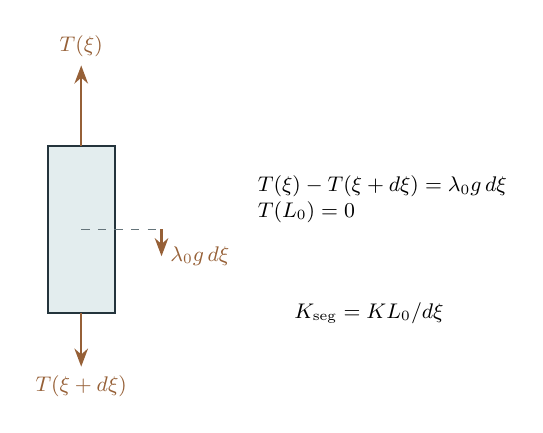
\begin{tikzpicture}[scale=.85,transform shape]

\fill[accent!12] (0,0) rectangle (1,-2.5);
\draw[object] (0,0) rectangle (1,-2.5);
\draw[force] (.5,0)--(.5,1.2) node[above] {$T(\xi)$};
\draw[force] (.5,-2.5)--(.5,-3.3) node[below] {$T(\xi+d\xi)$};
\draw[guide] (.5,-1.25)--(1.7,-1.25);
\draw[force,color=warm] (1.7,-1.25)--(1.7,-1.65) node[right] {$\lambda_0g\,d\xi$};
\node[align=left] at (5,-.8) {$T(\xi)-T(\xi+d\xi)=\lambda_0g\,d\xi$\\$T(L_0)=0$};
\node at (4.8,-2.5) {$K_{\rm seg}=KL_0/d\xi$};

\end{tikzpicture}
\figcaption{解图综三.3A\quad 一个材料微段的两端张力与重力；图中微段长度已经放大。}
\end{minipage}\end{center}
可把$\xi$想成刻在材料上的尺，读数一直跟随同一个材料点；外部固定的空间尺读数$x$记录该点在悬挂后的实际位置。自然长度微元$\mathrm d\xi$对应不变质量$\lambda_0\mathrm d\xi$，伸长后它占据$\mathrm dx=\mathrm d\xi+\mathrm d(\Delta\ell)$。因而求伸长与求密度共用同一个材料映射，长度微元随形变改变，质量保留。

解图综三.3A中，截面$\xi$以下的材料质量为$\lambda_0(L_0-\xi)$。它的重力由该截面张力承担，故
\[
T(\xi)=\lambda_0g(L_0-\xi).
\]
同样，图A的单个微段在静力平衡下满足$T(\xi)=T(\xi+\mathrm d\xi)+\lambda_0g\mathrm d\xi$，所以$\mathrm dT/\mathrm d\xi=-\lambda_0g$。从自由下端$T(L_0)=0$积分，也得到上述截面张力。上端张力为$mg$，下端为零，截面张力随其下方剩余材料质量从$mg$连续降到零。自然长度为$d\xi$的小段，其劲度系数为$KL_0/d\xi$。记恒定截面积为$S$，这个比例也可由杨氏模量导出：均匀端拉时应力为$F/S$、工程应变为$\Delta L/L_0$，故$E=FL_0/(S\Delta L)=KL_0/S$。轴向刚度$ES=KL_0$，对微段使用$T/S=E\,\mathrm d(\Delta\ell)/\mathrm d\xi$，即得微段劲度$ES/\mathrm d\xi$。因此该段伸长
\[
d(\Delta\ell)=\frac{T(\xi)}{KL_0}\,d\xi.
\]
将全杆看作这些串联小段并积分，得到
\[
\Delta L=\frac1{KL_0}\int_0^{L_0}\frac{mg}{L_0}(L_0-\xi)\,d\xi
=\boxed{\frac{mg}{2K}}.
\]
积分中的$\int_0^{L_0}(L_0-\xi)\mathrm d\xi=L_0^2/2$，与前面的$mg/(KL_0^2)$相乘，给$mg/(2K)$。上方小段承担下方全部材料重量，下方小段只承担更少重量，累积伸长按这种线性下降的张力积分。它等于把平均拉力$mg/2$作用于整根杆所得的伸长。这里的平均是对自然长度积分的结果，局部伸长使用各截面的实际张力。

为求密度，先保留一般参数$\alpha=mg/(KL_0)$。局部伸长比由原长加伸长给出，$\mathrm dx/\mathrm d\xi=1+T/(KL_0)=1+\alpha(1-\xi/L_0)$。它在上端为$1+\alpha$，在下端为1。把从上端到材料点的所有微段长度相加，得到该点的实际位置。从上端累积局部伸长，得
\[
x(\xi)=\int_0^\xi\left[1+\alpha\left(1-\frac{\eta}{L_0}\right)\right]d\eta
=(1+\alpha)\xi-\frac{\alpha\xi^2}{2L_0},
\quad
\frac{dx}{d\xi}=1+\alpha-\frac{\alpha\xi}{L_0}>0.
\]
\begin{center}\begin{minipage}{.98\linewidth}\centering
\begin{tikzpicture}[scale=.8,transform shape]
\draw[axis] (0,0)--(10.7,0) node[right] {$\xi/L_0$};
\draw[axis] (0,0)--(0,3.2) node[above] {$x/L_0$};\foreach \y/\lab in {0/0,0.9/.5,1.8/1,2.7/1.5}{\draw[thin] (0,\y)--(-.08,\y) node[left] {$\lab$};}
\node[above] at (5,3.5) {材料标签到空间位置的映射，题设$\alpha=1$};
\draw[traj] plot coordinates {(0.000000000,0.000000000) (0.083333333,0.029937500) (0.166666667,0.059750000) (0.250000000,0.089437500) (0.333333333,0.119000000) (0.416666667,0.148437500) (0.500000000,0.177750000) (0.583333333,0.206937500) (0.666666667,0.236000000) (0.750000000,0.264937500) (0.833333333,0.293750000) (0.916666667,0.322437500) (1.000000000,0.351000000) (1.083333333,0.379437500) (1.166666667,0.407750000) (1.250000000,0.435937500) (1.333333333,0.464000000) (1.416666667,0.491937500) (1.500000000,0.519750000) (1.583333333,0.547437500) (1.666666667,0.575000000) (1.750000000,0.602437500) (1.833333333,0.629750000) (1.916666667,0.656937500) (2.000000000,0.684000000) (2.083333333,0.710937500) (2.166666667,0.737750000) (2.250000000,0.764437500) (2.333333333,0.791000000) (2.416666667,0.817437500) (2.500000000,0.843750000) (2.583333333,0.869937500) (2.666666667,0.896000000) (2.750000000,0.921937500) (2.833333333,0.947750000) (2.916666667,0.973437500) (3.000000000,0.999000000) (3.083333333,1.024437500) (3.166666667,1.049750000) (3.250000000,1.074937500) (3.333333333,1.100000000) (3.416666667,1.124937500) (3.500000000,1.149750000) (3.583333333,1.174437500) (3.666666667,1.199000000) (3.750000000,1.223437500) (3.833333333,1.247750000) (3.916666667,1.271937500) (4.000000000,1.296000000) (4.083333333,1.319937500) (4.166666667,1.343750000) (4.250000000,1.367437500) (4.333333333,1.391000000) (4.416666667,1.414437500) (4.500000000,1.437750000) (4.583333333,1.460937500) (4.666666667,1.484000000) (4.750000000,1.506937500) (4.833333333,1.529750000) (4.916666667,1.552437500) (5.000000000,1.575000000) (5.083333333,1.597437500) (5.166666667,1.619750000) (5.250000000,1.641937500) (5.333333333,1.664000000) (5.416666667,1.685937500) (5.500000000,1.707750000) (5.583333333,1.729437500) (5.666666667,1.751000000) (5.750000000,1.772437500) (5.833333333,1.793750000) (5.916666667,1.814937500) (6.000000000,1.836000000) (6.083333333,1.856937500) (6.166666667,1.877750000) (6.250000000,1.898437500) (6.333333333,1.919000000) (6.416666667,1.939437500) (6.500000000,1.959750000) (6.583333333,1.979937500) (6.666666667,2.000000000) (6.750000000,2.019937500) (6.833333333,2.039750000) (6.916666667,2.059437500) (7.000000000,2.079000000) (7.083333333,2.098437500) (7.166666667,2.117750000) (7.250000000,2.136937500) (7.333333333,2.156000000) (7.416666667,2.174937500) (7.500000000,2.193750000) (7.583333333,2.212437500) (7.666666667,2.231000000) (7.750000000,2.249437500) (7.833333333,2.267750000) (7.916666667,2.285937500) (8.000000000,2.304000000) (8.083333333,2.321937500) (8.166666667,2.339750000) (8.250000000,2.357437500) (8.333333333,2.375000000) (8.416666667,2.392437500) (8.500000000,2.409750000) (8.583333333,2.426937500) (8.666666667,2.444000000) (8.750000000,2.460937500) (8.833333333,2.477750000) (8.916666667,2.494437500) (9.000000000,2.511000000) (9.083333333,2.527437500) (9.166666667,2.543750000) (9.250000000,2.559937500) (9.333333333,2.576000000) (9.416666667,2.591937500) (9.500000000,2.607750000) (9.583333333,2.623437500) (9.666666667,2.639000000) (9.750000000,2.654437500) (9.833333333,2.669750000) (9.916666667,2.684937500) (10.000000000,2.700000000)};
\node[below] at (0,-.12) {$0$};
\node[below] at (5,-.12) {$1/2$};
\node[below] at (10,-.12) {$1$};
\end{tikzpicture}
\figcaption{解图综三.3B\quad 材料标签到空间位置的映射，题设$\alpha=1$}
\end{minipage}\end{center}
解图综三.3B中同一质量元满足$\lambda(x)\,dx=\lambda_0\,d\xi$，所以
\[
\lambda(x(\xi))=\frac{\lambda_0}{1+\alpha-\alpha\xi/L_0}.
\]
相同质量在空间中被拉长得越多，单位空间长度内的质量就越少；因此密度除以局部伸长比。上式仍把密度对应到材料标签$\xi$，实际问题则使用固定尺读出的$x$。要把密度写成实际位置的函数，还须从映射中解出材料坐标。解二次方程，并取满足$x=0$时$\xi=0$的根，
\[
\xi=\frac{L_0}{\alpha}
\left[1+\alpha-\sqrt{(1+\alpha)^2-\frac{2\alpha x}{L_0}}\right].
\]
映射的导数始终为正，故$\xi$从0增加到$L_0$时，$x$从0单调增加到$L_0(1+\alpha/2)$，逆映射在这一区间唯一。代回后，分母$1+\alpha-\alpha\xi/L_0$恰变为二次根式中的平方根；其符号由正伸长比固定。代回雅可比，得到空间坐标下的分布
\[
\boxed{\lambda(x)=
\frac{m}{L_0\sqrt{(1+\alpha)^2-2\alpha x/L_0}}},
\quad 0\le x\le L_0(1+\alpha/2).
\]
所取根连续连接$\xi=0$的上端，并随$x$增加到$\xi=L_0$的下端。
\begin{center}\begin{minipage}{.98\linewidth}\centering
\begin{tikzpicture}[scale=.8,transform shape]
\draw[axis] (0,0)--(10.7,0) node[right] {$x/L_0$};
\draw[axis] (0,0)--(0,3.2) node[above] {$\lambda/\lambda_0$};
\node[above] at (5,3.5) {上端密度为$1/2$，下端恢复自然值1};
\draw[traj] plot coordinates {(0.000000000,1.400000000) (0.083333333,1.404395615) (0.166666667,1.408832895) (0.250000000,1.413312502) (0.333333333,1.417835114) (0.416666667,1.422401422) (0.500000000,1.427012136) (0.583333333,1.431667979) (0.666666667,1.436369693) (0.750000000,1.441118035) (0.833333333,1.445913783) (0.916666667,1.450757728) (1.000000000,1.455650686) (1.083333333,1.460593487) (1.166666667,1.465586983) (1.250000000,1.470632048) (1.333333333,1.475729575) (1.416666667,1.480880479) (1.500000000,1.486085699) (1.583333333,1.491346196) (1.666666667,1.496662955) (1.750000000,1.502036986) (1.833333333,1.507469326) (1.916666667,1.512961035) (2.000000000,1.518513205) (2.083333333,1.524126951) (2.166666667,1.529803421) (2.250000000,1.535543792) (2.333333333,1.541349271) (2.416666667,1.547221099) (2.500000000,1.553160549) (2.583333333,1.559168930) (2.666666667,1.565247584) (2.750000000,1.571397893) (2.833333333,1.577621275) (2.916666667,1.583919190) (3.000000000,1.590293136) (3.083333333,1.596744656) (3.166666667,1.603275336) (3.250000000,1.609886809) (3.333333333,1.616580754) (3.416666667,1.623358900) (3.500000000,1.630223027) (3.583333333,1.637174969) (3.666666667,1.644216615) (3.750000000,1.651349909) (3.833333333,1.658576858) (3.916666667,1.665899528) (4.000000000,1.673320053) (4.083333333,1.680840631) (4.166666667,1.688463530) (4.250000000,1.696191092) (4.333333333,1.704025734) (4.416666667,1.711969953) (4.500000000,1.720026327) (4.583333333,1.728197520) (4.666666667,1.736486284) (4.750000000,1.744895468) (4.833333333,1.753428015) (4.916666667,1.762086971) (5.000000000,1.770875490) (5.083333333,1.779796833) (5.166666667,1.788854382) (5.250000000,1.798051637) (5.333333333,1.807392228) (5.416666667,1.816879917) (5.500000000,1.826518605) (5.583333333,1.836312340) (5.666666667,1.846265326) (5.750000000,1.856381924) (5.833333333,1.866666667) (5.916666667,1.877124265) (6.000000000,1.887759615) (6.083333333,1.898577810) (6.166666667,1.909584151) (6.250000000,1.920784154) (6.333333333,1.932183566) (6.416666667,1.943788377) (6.500000000,1.955604828) (6.583333333,1.967639433) (6.666666667,1.979898987) (6.750000000,1.992390588) (6.833333333,2.005121647) (6.916666667,2.018099916) (7.000000000,2.031333500) (7.083333333,2.044830881) (7.166666667,2.058600942) (7.250000000,2.072652989) (7.333333333,2.086996779) (7.416666667,2.101642550) (7.500000000,2.116601049) (7.583333333,2.131883565) (7.666666667,2.147501969) (7.750000000,2.163468746) (7.833333333,2.179797044) (7.916666667,2.196500714) (8.000000000,2.213594362) (8.083333333,2.231093404) (8.166666667,2.249014121) (8.250000000,2.267373725) (8.333333333,2.286190427) (8.416666667,2.305483515) (8.500000000,2.325273436) (8.583333333,2.345581886) (8.666666667,2.366431913) (8.750000000,2.387848023) (8.833333333,2.409856304) (8.916666667,2.432484559) (9.000000000,2.455762454) (9.083333333,2.479721680) (9.166666667,2.504396135) (9.250000000,2.529822128) (9.333333333,2.556038602) (9.416666667,2.583087382) (9.500000000,2.611013463) (9.583333333,2.639865316) (9.666666667,2.669695250) (9.750000000,2.700559804) (9.833333333,2.732520204) (9.916666667,2.765642871) (10.000000000,2.800000000)};
\node[below] at (0,-.12) {$0$};
\node[below] at (6.666666666666667,-.12) {$1$};
\node[below] at (10,-.12) {$3/2$};
\node[left] at (0,1.4) {$1/2$};\node[left] at (0,2.8) {$1$};
\end{tikzpicture}
\figcaption{解图综三.3C\quad 上端密度为$1/2$，下端恢复自然值1}
\end{minipage}\end{center}
取题设$K=mg/L_0$，即$\alpha=1$，解图综三.3C中的曲线为
\[
\boxed{\lambda(x)=\frac{m}{L_0\sqrt{4-2x/L_0}}},
\qquad \boxed{0\le x\le\frac32L_0}.
\]
上端被拉得最疏，$\lambda(0)=m/(2L_0)$；下端张力为零，$\lambda(3L_0/2)=m/L_0$。积分实际空间密度得到总质量：
\[
\int_0^{3L_0/2}\lambda(x)\,dx
=m\left[-\sqrt{4-2x/L_0}\right]_0^{3L_0/2}=m.
\]
各段质量固定，伸长最大的上半部线密度较低。解图综三.3B 中材料坐标 $\xi=L_0/2$ 恰好平分质量；代入位置函数得 $x=L_0(1/2+3\alpha/8)$，比伸长后的长度中点 $L_0(1/2+\alpha/4)$ 低 $\alpha L_0/8$。题设 $\alpha=1$ 时上端工程应变为 $1$，这里按给定的线性拉伸关系和不变截面计算。
在一般参数下，空间下端的根式化为$\sqrt{(1+\alpha)^2-2\alpha(1+\alpha/2)}=1$，所以自由端恢复自然线密度；上端根式为$1+\alpha$，对应最大伸长比。

也可沿空间坐标理解静力平衡：$\mathrm dT/\mathrm dx=(\mathrm dT/\mathrm d\xi)/(\mathrm dx/\mathrm d\xi)=-g\lambda(x)$，表示上、下截面张力差支撑实际微段的重量。材料坐标中的常量质量密度与空间坐标中的变密度，通过相同伸长比相连。全长积分使用空间下端$3L_0/2$，上端和下端密度分别对应最大应变与零应变，三者都由映射的两端条件给出。



\Needspace{8\baselineskip}

\pdfbookmark[3]{关键洞察}{q3-h5}

\subsection*{关键洞察}

自然尺的读数跟随材料点保持相同，空间尺的读数则反映形变后的实际位置。总伸长的二分之一来自张力沿自然长度的线性下降。换成实际位置后，张力导数为$\mathrm dT/\mathrm dx=-g\lambda(x)$，仍表示每个实际小段的静力平衡；密度的非均匀性与两种坐标描述同一材料相容。

\Needspace{8\baselineskip}

\pdfbookmark[3]{易错点}{q3-h6}

\subsection*{易错点}

微段自然长度变短时劲度系数相应增大，应用$ES=KL_0$保留长度因子。密度以实际长度为分母，先由$\lambda\mathrm dx=\lambda_0\mathrm d\xi$得到参数式，再完成坐标替换。上端条件$x=0,\xi=0$选定逆映射的根，空间定义域由$\xi=L_0$的像给出。题设参数对应上端单位工程应变，结果采用给定的理想线弹性及面积不变模型。

\Needspace{8\baselineskip}

\pdfbookmark[3]{课堂讲解建议}{q3-h7}

\subsection*{课堂讲解建议}

让学生先把自然尺和空间尺重叠，再拉伸材料尺，标出同一个小色块的两个读数。三个截面依次列下方材料质量，以此预测上端张力最大、上端密度最低。追问：“材料点$\xi$以下还剩多少质量？”答为$\lambda_0(L_0-\xi)$，它按材料标签计数。再问：“相同质量色块在哪一端更长？”上端张力较大、伸长更多，故空间线密度较小；实际长度与自然密度相乘则不能表示该段质量。

微段公式写出后，要求说明自然长度$\mathrm d\xi$为何出现在应变分母中，并由整杆劲度求微段劲度。画图B时先确定两端斜率和下端位置，再由图C比较同质量微段在空间中占据的长度。最后按实际全长积分质量，分别计算两端密度，结合上端应变说明题设模型采用的范围。

\Needspace{8\baselineskip}

\pdfbookmark[3]{变式训练}{q3-h8}

\subsection*{变式训练}

\begin{enumerate}
\Needspace{20\baselineskip}
\item 保留任意$\alpha=mg/(KL_0)>0$，求总长、两端密度与弱重力极限。
\textbf{解：}变图综三.3V1由$x=(1+\alpha)\xi-\alpha\xi^2/(2L_0)$，下端总长$L=L_0(1+\alpha/2)$。局部伸长比为$1+\alpha-\alpha\xi/L_0$，所以两端密度分别为$\lambda_0/(1+\alpha)$和$\lambda_0$，内部空间分布为$\lambda(x)=\lambda_0/\sqrt{(1+\alpha)^2-2\alpha x/L_0}$。$\alpha\to0$时$x\to\xi$且密度趋于均匀；固定空间位置的一阶展开为$\lambda/\lambda_0\simeq1-\alpha(1-x/L_0)$。
\begin{center}\begin{minipage}{.98\linewidth}\centering
\begin{tikzpicture}[scale=.8,transform shape]
\draw[axis] (0,0)--(10.7,0) node[right] {$\alpha$};
\draw[axis] (0,0)--(0,3.2) node[above] {$\lambda_t/\lambda_0$};\foreach \y/\lab in {0/0,1.4/.5,2.8/1}{\draw[thin] (0,\y)--(-.08,\y) node[left] {$\lab$};}
\node[above] at (5,3.5) {重力与弹性刚度之比决定上端伸长比};
\draw[traj] plot coordinates {(0.000000000,2.800000000) (0.083333333,2.731707317) (0.166666667,2.666666667) (0.250000000,2.604651163) (0.333333333,2.545454545) (0.416666667,2.488888889) (0.500000000,2.434782609) (0.583333333,2.382978723) (0.666666667,2.333333333) (0.750000000,2.285714286) (0.833333333,2.240000000) (0.916666667,2.196078431) (1.000000000,2.153846154) (1.083333333,2.113207547) (1.166666667,2.074074074) (1.250000000,2.036363636) (1.333333333,2.000000000) (1.416666667,1.964912281) (1.500000000,1.931034483) (1.583333333,1.898305085) (1.666666667,1.866666667) (1.750000000,1.836065574) (1.833333333,1.806451613) (1.916666667,1.777777778) (2.000000000,1.750000000) (2.083333333,1.723076923) (2.166666667,1.696969697) (2.250000000,1.671641791) (2.333333333,1.647058824) (2.416666667,1.623188406) (2.500000000,1.600000000) (2.583333333,1.577464789) (2.666666667,1.555555556) (2.750000000,1.534246575) (2.833333333,1.513513514) (2.916666667,1.493333333) (3.000000000,1.473684211) (3.083333333,1.454545455) (3.166666667,1.435897436) (3.250000000,1.417721519) (3.333333333,1.400000000) (3.416666667,1.382716049) (3.500000000,1.365853659) (3.583333333,1.349397590) (3.666666667,1.333333333) (3.750000000,1.317647059) (3.833333333,1.302325581) (3.916666667,1.287356322) (4.000000000,1.272727273) (4.083333333,1.258426966) (4.166666667,1.244444444) (4.250000000,1.230769231) (4.333333333,1.217391304) (4.416666667,1.204301075) (4.500000000,1.191489362) (4.583333333,1.178947368) (4.666666667,1.166666667) (4.750000000,1.154639175) (4.833333333,1.142857143) (4.916666667,1.131313131) (5.000000000,1.120000000) (5.083333333,1.108910891) (5.166666667,1.098039216) (5.250000000,1.087378641) (5.333333333,1.076923077) (5.416666667,1.066666667) (5.500000000,1.056603774) (5.583333333,1.046728972) (5.666666667,1.037037037) (5.750000000,1.027522936) (5.833333333,1.018181818) (5.916666667,1.009009009) (6.000000000,1.000000000) (6.083333333,0.991150442) (6.166666667,0.982456140) (6.250000000,0.973913043) (6.333333333,0.965517241) (6.416666667,0.957264957) (6.500000000,0.949152542) (6.583333333,0.941176471) (6.666666667,0.933333333) (6.750000000,0.925619835) (6.833333333,0.918032787) (6.916666667,0.910569106) (7.000000000,0.903225806) (7.083333333,0.896000000) (7.166666667,0.888888889) (7.250000000,0.881889764) (7.333333333,0.875000000) (7.416666667,0.868217054) (7.500000000,0.861538462) (7.583333333,0.854961832) (7.666666667,0.848484848) (7.750000000,0.842105263) (7.833333333,0.835820896) (7.916666667,0.829629630) (8.000000000,0.823529412) (8.083333333,0.817518248) (8.166666667,0.811594203) (8.250000000,0.805755396) (8.333333333,0.800000000) (8.416666667,0.794326241) (8.500000000,0.788732394) (8.583333333,0.783216783) (8.666666667,0.777777778) (8.750000000,0.772413793) (8.833333333,0.767123288) (8.916666667,0.761904762) (9.000000000,0.756756757) (9.083333333,0.751677852) (9.166666667,0.746666667) (9.250000000,0.741721854) (9.333333333,0.736842105) (9.416666667,0.732026144) (9.500000000,0.727272727) (9.583333333,0.722580645) (9.666666667,0.717948718) (9.750000000,0.713375796) (9.833333333,0.708860759) (9.916666667,0.704402516) (10.000000000,0.700000000)};
\node[below] at (0,-.12) {$0$};
\node[below] at (3.3333333333333335,-.12) {$1$};
\node[below] at (10,-.12) {$3$};
\end{tikzpicture}
\figcaption{变图综三.3V1\quad 重力与弹性刚度之比决定上端伸长比}
\end{minipage}\end{center}

\Needspace{20\baselineskip}
\item 杆下端另挂质量$M$，求伸长、实际位置映射及空间密度。
\textbf{解：}变图综三.3V2截面张力为$[M+m(1-\xi/L_0)]g$。令$b=Mg/(KL_0)$，局部伸长比为$1+b+\alpha-\alpha\xi/L_0$，积分得$x=(1+b+\alpha)\xi-\alpha\xi^2/(2L_0)$，故$\Delta L=(M+m/2)g/K$。质量守恒与逆映射给$\lambda(x)=\lambda_0/\sqrt{(1+b+\alpha)^2-2\alpha x/L_0}$，范围$0\le x\le L_0(1+b+\alpha/2)$。下端仍受$Mg$，密度为$\lambda_0/(1+b)$；上端为$\lambda_0/(1+b+\alpha)$。
\begin{center}\begin{minipage}{.98\linewidth}\centering
\begin{tikzpicture}[scale=.8,transform shape]
\draw[axis] (0,0)--(10.7,0) node[right] {$x/L_0$};
\draw[axis] (0,0)--(0,3.2) node[above] {$\lambda/\lambda_0$};\foreach \y/\lab in {1.6/.4,2/{1/2},2.6666666666666665/{2/3}}{\draw[thin] (0,\y)--(-.08,\y) node[left] {$\lab$};}
\node[above] at (5,3.5) {示例$\alpha=1,b=1/2$：下端负载也拉伸底部材料};
\draw[traj] plot coordinates {(0.000000000,1.600000000) (0.103993056,1.605351171) (0.207638889,1.610738255) (0.310937500,1.616161616) (0.413888889,1.621621622) (0.516493056,1.627118644) (0.618750000,1.632653061) (0.720659722,1.638225256) (0.822222222,1.643835616) (0.923437500,1.649484536) (1.024305556,1.655172414) (1.124826389,1.660899654) (1.225000000,1.666666667) (1.324826389,1.672473868) (1.424305556,1.678321678) (1.523437500,1.684210526) (1.622222222,1.690140845) (1.720659722,1.696113074) (1.818750000,1.702127660) (1.916493056,1.708185053) (2.013888889,1.714285714) (2.110937500,1.720430108) (2.207638889,1.726618705) (2.303993056,1.732851986) (2.400000000,1.739130435) (2.495659722,1.745454545) (2.590972222,1.751824818) (2.685937500,1.758241758) (2.780555556,1.764705882) (2.874826389,1.771217712) (2.968750000,1.777777778) (3.062326389,1.784386617) (3.155555556,1.791044776) (3.248437500,1.797752809) (3.340972222,1.804511278) (3.433159722,1.811320755) (3.525000000,1.818181818) (3.616493056,1.825095057) (3.707638889,1.832061069) (3.798437500,1.839080460) (3.888888889,1.846153846) (3.978993056,1.853281853) (4.068750000,1.860465116) (4.158159722,1.867704280) (4.247222222,1.875000000) (4.335937500,1.882352941) (4.424305556,1.889763780) (4.512326389,1.897233202) (4.600000000,1.904761905) (4.687326389,1.912350598) (4.774305556,1.920000000) (4.860937500,1.927710843) (4.947222222,1.935483871) (5.033159722,1.943319838) (5.118750000,1.951219512) (5.203993056,1.959183673) (5.288888889,1.967213115) (5.373437500,1.975308642) (5.457638889,1.983471074) (5.541493056,1.991701245) (5.625000000,2.000000000) (5.708159722,2.008368201) (5.790972222,2.016806723) (5.873437500,2.025316456) (5.955555556,2.033898305) (6.037326389,2.042553191) (6.118750000,2.051282051) (6.199826389,2.060085837) (6.280555556,2.068965517) (6.360937500,2.077922078) (6.440972222,2.086956522) (6.520659722,2.096069869) (6.600000000,2.105263158) (6.678993056,2.114537445) (6.757638889,2.123893805) (6.835937500,2.133333333) (6.913888889,2.142857143) (6.991493056,2.152466368) (7.068750000,2.162162162) (7.145659722,2.171945701) (7.222222222,2.181818182) (7.298437500,2.191780822) (7.374305556,2.201834862) (7.449826389,2.211981567) (7.525000000,2.222222222) (7.599826389,2.232558140) (7.674305556,2.242990654) (7.748437500,2.253521127) (7.822222222,2.264150943) (7.895659722,2.274881517) (7.968750000,2.285714286) (8.041493056,2.296650718) (8.113888889,2.307692308) (8.185937500,2.318840580) (8.257638889,2.330097087) (8.328993056,2.341463415) (8.400000000,2.352941176) (8.470659722,2.364532020) (8.540972222,2.376237624) (8.610937500,2.388059701) (8.680555556,2.400000000) (8.749826389,2.412060302) (8.818750000,2.424242424) (8.887326389,2.436548223) (8.955555556,2.448979592) (9.023437500,2.461538462) (9.090972222,2.474226804) (9.158159722,2.487046632) (9.225000000,2.500000000) (9.291493056,2.513089005) (9.357638889,2.526315789) (9.423437500,2.539682540) (9.488888889,2.553191489) (9.553993056,2.566844920) (9.618750000,2.580645161) (9.683159722,2.594594595) (9.747222222,2.608695652) (9.810937500,2.622950820) (9.874305556,2.637362637) (9.937326389,2.651933702) (10.000000000,2.666666667)};
\node[below] at (0,-.12) {$0$};
\node[below] at (5,-.12) {$1$};
\node[below] at (10,-.12) {$2$};
\end{tikzpicture}
\figcaption{变图综三.3V2\quad 示例$\alpha=1,b=1/2$：下端负载也拉伸底部材料}
\end{minipage}\end{center}

\Needspace{20\baselineskip}
\item 求悬挂杆的质心，并比较它与实际杆长中点。
\textbf{解：}变图综三.3V3以材料微元$\mathrm dm=(m/L_0)\mathrm d\xi$积分，$x_{\rm cm}=m^{-1}\int x\,\mathrm dm=L_0^{-1}\int_0^{L_0}[(1+\alpha)\xi-\alpha\xi^2/(2L_0)]\mathrm d\xi=L_0(1/2+\alpha/3)$。实际杆长的一半为$L/2=L_0(1/2+\alpha/4)$，所以质心在中点下方$\alpha L_0/12$。下方材料伸长较少、空间密度较高，使相同长度区段在下部包含更多质量。
\begin{center}\begin{minipage}{.98\linewidth}\centering
\begin{tikzpicture}[scale=.8,transform shape]
\draw[axis] (0,0)--(10.7,0) node[right] {$\alpha$};
\draw[axis] (0,0)--(0,3.2) node[above] {位置除以$L_0$};\foreach \y/\lab in {0.9/.5,1.8/1,2.7/1.5}{\draw[thin] (0,\y)--(-.08,\y) node[left] {$\lab$};}
\node[above] at (5,3.5) {实线质心，虚线杆长中点；$\alpha>0$时质心位于其下方};
\draw[traj] plot coordinates {(0.000000000,0.900000000) (0.083333333,0.915000000) (0.166666667,0.930000000) (0.250000000,0.945000000) (0.333333333,0.960000000) (0.416666667,0.975000000) (0.500000000,0.990000000) (0.583333333,1.005000000) (0.666666667,1.020000000) (0.750000000,1.035000000) (0.833333333,1.050000000) (0.916666667,1.065000000) (1.000000000,1.080000000) (1.083333333,1.095000000) (1.166666667,1.110000000) (1.250000000,1.125000000) (1.333333333,1.140000000) (1.416666667,1.155000000) (1.500000000,1.170000000) (1.583333333,1.185000000) (1.666666667,1.200000000) (1.750000000,1.215000000) (1.833333333,1.230000000) (1.916666667,1.245000000) (2.000000000,1.260000000) (2.083333333,1.275000000) (2.166666667,1.290000000) (2.250000000,1.305000000) (2.333333333,1.320000000) (2.416666667,1.335000000) (2.500000000,1.350000000) (2.583333333,1.365000000) (2.666666667,1.380000000) (2.750000000,1.395000000) (2.833333333,1.410000000) (2.916666667,1.425000000) (3.000000000,1.440000000) (3.083333333,1.455000000) (3.166666667,1.470000000) (3.250000000,1.485000000) (3.333333333,1.500000000) (3.416666667,1.515000000) (3.500000000,1.530000000) (3.583333333,1.545000000) (3.666666667,1.560000000) (3.750000000,1.575000000) (3.833333333,1.590000000) (3.916666667,1.605000000) (4.000000000,1.620000000) (4.083333333,1.635000000) (4.166666667,1.650000000) (4.250000000,1.665000000) (4.333333333,1.680000000) (4.416666667,1.695000000) (4.500000000,1.710000000) (4.583333333,1.725000000) (4.666666667,1.740000000) (4.750000000,1.755000000) (4.833333333,1.770000000) (4.916666667,1.785000000) (5.000000000,1.800000000) (5.083333333,1.815000000) (5.166666667,1.830000000) (5.250000000,1.845000000) (5.333333333,1.860000000) (5.416666667,1.875000000) (5.500000000,1.890000000) (5.583333333,1.905000000) (5.666666667,1.920000000) (5.750000000,1.935000000) (5.833333333,1.950000000) (5.916666667,1.965000000) (6.000000000,1.980000000) (6.083333333,1.995000000) (6.166666667,2.010000000) (6.250000000,2.025000000) (6.333333333,2.040000000) (6.416666667,2.055000000) (6.500000000,2.070000000) (6.583333333,2.085000000) (6.666666667,2.100000000) (6.750000000,2.115000000) (6.833333333,2.130000000) (6.916666667,2.145000000) (7.000000000,2.160000000) (7.083333333,2.175000000) (7.166666667,2.190000000) (7.250000000,2.205000000) (7.333333333,2.220000000) (7.416666667,2.235000000) (7.500000000,2.250000000) (7.583333333,2.265000000) (7.666666667,2.280000000) (7.750000000,2.295000000) (7.833333333,2.310000000) (7.916666667,2.325000000) (8.000000000,2.340000000) (8.083333333,2.355000000) (8.166666667,2.370000000) (8.250000000,2.385000000) (8.333333333,2.400000000) (8.416666667,2.415000000) (8.500000000,2.430000000) (8.583333333,2.445000000) (8.666666667,2.460000000) (8.750000000,2.475000000) (8.833333333,2.490000000) (8.916666667,2.505000000) (9.000000000,2.520000000) (9.083333333,2.535000000) (9.166666667,2.550000000) (9.250000000,2.565000000) (9.333333333,2.580000000) (9.416666667,2.595000000) (9.500000000,2.610000000) (9.583333333,2.625000000) (9.666666667,2.640000000) (9.750000000,2.655000000) (9.833333333,2.670000000) (9.916666667,2.685000000) (10.000000000,2.700000000)};
\draw[dashed,thick,color=warm] plot coordinates {(0.000000000,0.900000000) (0.083333333,0.911250000) (0.166666667,0.922500000) (0.250000000,0.933750000) (0.333333333,0.945000000) (0.416666667,0.956250000) (0.500000000,0.967500000) (0.583333333,0.978750000) (0.666666667,0.990000000) (0.750000000,1.001250000) (0.833333333,1.012500000) (0.916666667,1.023750000) (1.000000000,1.035000000) (1.083333333,1.046250000) (1.166666667,1.057500000) (1.250000000,1.068750000) (1.333333333,1.080000000) (1.416666667,1.091250000) (1.500000000,1.102500000) (1.583333333,1.113750000) (1.666666667,1.125000000) (1.750000000,1.136250000) (1.833333333,1.147500000) (1.916666667,1.158750000) (2.000000000,1.170000000) (2.083333333,1.181250000) (2.166666667,1.192500000) (2.250000000,1.203750000) (2.333333333,1.215000000) (2.416666667,1.226250000) (2.500000000,1.237500000) (2.583333333,1.248750000) (2.666666667,1.260000000) (2.750000000,1.271250000) (2.833333333,1.282500000) (2.916666667,1.293750000) (3.000000000,1.305000000) (3.083333333,1.316250000) (3.166666667,1.327500000) (3.250000000,1.338750000) (3.333333333,1.350000000) (3.416666667,1.361250000) (3.500000000,1.372500000) (3.583333333,1.383750000) (3.666666667,1.395000000) (3.750000000,1.406250000) (3.833333333,1.417500000) (3.916666667,1.428750000) (4.000000000,1.440000000) (4.083333333,1.451250000) (4.166666667,1.462500000) (4.250000000,1.473750000) (4.333333333,1.485000000) (4.416666667,1.496250000) (4.500000000,1.507500000) (4.583333333,1.518750000) (4.666666667,1.530000000) (4.750000000,1.541250000) (4.833333333,1.552500000) (4.916666667,1.563750000) (5.000000000,1.575000000) (5.083333333,1.586250000) (5.166666667,1.597500000) (5.250000000,1.608750000) (5.333333333,1.620000000) (5.416666667,1.631250000) (5.500000000,1.642500000) (5.583333333,1.653750000) (5.666666667,1.665000000) (5.750000000,1.676250000) (5.833333333,1.687500000) (5.916666667,1.698750000) (6.000000000,1.710000000) (6.083333333,1.721250000) (6.166666667,1.732500000) (6.250000000,1.743750000) (6.333333333,1.755000000) (6.416666667,1.766250000) (6.500000000,1.777500000) (6.583333333,1.788750000) (6.666666667,1.800000000) (6.750000000,1.811250000) (6.833333333,1.822500000) (6.916666667,1.833750000) (7.000000000,1.845000000) (7.083333333,1.856250000) (7.166666667,1.867500000) (7.250000000,1.878750000) (7.333333333,1.890000000) (7.416666667,1.901250000) (7.500000000,1.912500000) (7.583333333,1.923750000) (7.666666667,1.935000000) (7.750000000,1.946250000) (7.833333333,1.957500000) (7.916666667,1.968750000) (8.000000000,1.980000000) (8.083333333,1.991250000) (8.166666667,2.002500000) (8.250000000,2.013750000) (8.333333333,2.025000000) (8.416666667,2.036250000) (8.500000000,2.047500000) (8.583333333,2.058750000) (8.666666667,2.070000000) (8.750000000,2.081250000) (8.833333333,2.092500000) (8.916666667,2.103750000) (9.000000000,2.115000000) (9.083333333,2.126250000) (9.166666667,2.137500000) (9.250000000,2.148750000) (9.333333333,2.160000000) (9.416666667,2.171250000) (9.500000000,2.182500000) (9.583333333,2.193750000) (9.666666667,2.205000000) (9.750000000,2.216250000) (9.833333333,2.227500000) (9.916666667,2.238750000) (10.000000000,2.250000000)};
\node[below] at (0,-.12) {$0$};
\node[below] at (3.3333333333333335,-.12) {$1$};
\node[below] at (10,-.12) {$3$};
\end{tikzpicture}
\figcaption{变图综三.3V3\quad 实线质心，虚线实际杆长中点，质心总在其下方}
\end{minipage}\end{center}

\Needspace{20\baselineskip}
\item 求杆在自重下的弹性储能，说明局部张力在能量积分中的作用。
\textbf{解：}变图综三.3V4微段相当于劲度$KL_0/\mathrm d\xi$的弹簧，能量为$\mathrm dU=T(\xi)^2\mathrm d\xi/(2KL_0)$。代入$T=mg(1-\xi/L_0)$并积分，$U=m^2g^2\int_0^{L_0}(1-\xi/L_0)^2\mathrm d\xi/(2KL_0)=m^2g^2/(6K)$。若把最大张力$mg$用于全部小段，会得到三倍能量；自重悬挂采用的是张力平方沿材料长度的实际平均值。
\begin{center}\begin{minipage}{.98\linewidth}\centering
\begin{tikzpicture}[scale=.8,transform shape]
\draw[axis] (0,0)--(10.7,0) node[right] {$\xi/L_0$};
\draw[axis] (0,0)--(0,3.2) node[above] {$2KL_0\,\mathrm dU/(m^2g^2\mathrm d\xi)$};\foreach \y/\lab in {0/0,1.4/.5,2.8/1}{\draw[thin] (0,\y)--(-.08,\y) node[left] {$\lab$};}
\node[above] at (5,3.5) {局部储能密度按张力平方分布};
\draw[traj] plot coordinates {(0.000000000,2.800000000) (0.083333333,2.753527778) (0.166666667,2.707444444) (0.250000000,2.661750000) (0.333333333,2.616444444) (0.416666667,2.571527778) (0.500000000,2.527000000) (0.583333333,2.482861111) (0.666666667,2.439111111) (0.750000000,2.395750000) (0.833333333,2.352777778) (0.916666667,2.310194444) (1.000000000,2.268000000) (1.083333333,2.226194444) (1.166666667,2.184777778) (1.250000000,2.143750000) (1.333333333,2.103111111) (1.416666667,2.062861111) (1.500000000,2.023000000) (1.583333333,1.983527778) (1.666666667,1.944444444) (1.750000000,1.905750000) (1.833333333,1.867444444) (1.916666667,1.829527778) (2.000000000,1.792000000) (2.083333333,1.754861111) (2.166666667,1.718111111) (2.250000000,1.681750000) (2.333333333,1.645777778) (2.416666667,1.610194444) (2.500000000,1.575000000) (2.583333333,1.540194444) (2.666666667,1.505777778) (2.750000000,1.471750000) (2.833333333,1.438111111) (2.916666667,1.404861111) (3.000000000,1.372000000) (3.083333333,1.339527778) (3.166666667,1.307444444) (3.250000000,1.275750000) (3.333333333,1.244444444) (3.416666667,1.213527778) (3.500000000,1.183000000) (3.583333333,1.152861111) (3.666666667,1.123111111) (3.750000000,1.093750000) (3.833333333,1.064777778) (3.916666667,1.036194444) (4.000000000,1.008000000) (4.083333333,0.980194444) (4.166666667,0.952777778) (4.250000000,0.925750000) (4.333333333,0.899111111) (4.416666667,0.872861111) (4.500000000,0.847000000) (4.583333333,0.821527778) (4.666666667,0.796444444) (4.750000000,0.771750000) (4.833333333,0.747444444) (4.916666667,0.723527778) (5.000000000,0.700000000) (5.083333333,0.676861111) (5.166666667,0.654111111) (5.250000000,0.631750000) (5.333333333,0.609777778) (5.416666667,0.588194444) (5.500000000,0.567000000) (5.583333333,0.546194444) (5.666666667,0.525777778) (5.750000000,0.505750000) (5.833333333,0.486111111) (5.916666667,0.466861111) (6.000000000,0.448000000) (6.083333333,0.429527778) (6.166666667,0.411444444) (6.250000000,0.393750000) (6.333333333,0.376444444) (6.416666667,0.359527778) (6.500000000,0.343000000) (6.583333333,0.326861111) (6.666666667,0.311111111) (6.750000000,0.295750000) (6.833333333,0.280777778) (6.916666667,0.266194444) (7.000000000,0.252000000) (7.083333333,0.238194444) (7.166666667,0.224777778) (7.250000000,0.211750000) (7.333333333,0.199111111) (7.416666667,0.186861111) (7.500000000,0.175000000) (7.583333333,0.163527778) (7.666666667,0.152444444) (7.750000000,0.141750000) (7.833333333,0.131444444) (7.916666667,0.121527778) (8.000000000,0.112000000) (8.083333333,0.102861111) (8.166666667,0.094111111) (8.250000000,0.085750000) (8.333333333,0.077777778) (8.416666667,0.070194444) (8.500000000,0.063000000) (8.583333333,0.056194444) (8.666666667,0.049777778) (8.750000000,0.043750000) (8.833333333,0.038111111) (8.916666667,0.032861111) (9.000000000,0.028000000) (9.083333333,0.023527778) (9.166666667,0.019444444) (9.250000000,0.015750000) (9.333333333,0.012444444) (9.416666667,0.009527778) (9.500000000,0.007000000) (9.583333333,0.004861111) (9.666666667,0.003111111) (9.750000000,0.001750000) (9.833333333,0.000777778) (9.916666667,0.000194444) (10.000000000,0.000000000)};
\node[below] at (0,-.12) {$0$};
\node[below] at (5,-.12) {$1/2$};
\node[below] at (10,-.12) {$1$};
\end{tikzpicture}
\figcaption{变图综三.3V4\quad 局部储能密度按张力平方分布}
\end{minipage}\end{center}

\Needspace{20\baselineskip}
\item 要求杆上各处密度至少为自然线密度的$\eta$倍，$0<\eta<1$，求$K$的限制，并算$\eta=0.95$时的最大相对伸长。
\textbf{解：}变图综三.3V5最低密度在上端，为$\lambda_0/(1+\alpha)$。条件$1/(1+\alpha)\ge\eta$给$\alpha\le\eta^{-1}-1$，因此$K\ge mg/[L_0(\eta^{-1}-1)]$。总相对伸长$\Delta L/L_0=\alpha/2\le(\eta^{-1}-1)/2$。当$\eta=0.95$时，$\alpha\le1/19$，$K\ge19mg/L_0$，相对伸长至多$1/38\approx2.63\%$。上端最大应变与这项密度要求直接对应。
\begin{center}\begin{minipage}{.98\linewidth}\centering
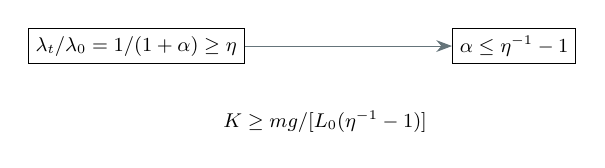
\begin{tikzpicture}[scale=.8,transform shape]
\node[draw] (a) at (0,0) {$\lambda_t/\lambda_0=1/(1+\alpha)\ge\eta$};\node[draw] (b) at (6,0) {$\alpha\le\eta^{-1}-1$};\draw[axis] (a)--(b);\node at (3,-1.2) {$K\ge mg/[L_0(\eta^{-1}-1)]$};
\end{tikzpicture}
\figcaption{变图综三.3V5\quad 上端最小密度把整杆的密度要求化为最大应变限制}
\end{minipage}\end{center}

\Needspace{20\baselineskip}
\item 用分布支承先把竖直杆保持为自然长度，上端固定后移去其余支承，经阻尼最终静止。求重力势能降低量与耗散能量。
\textbf{解：}变图综三.3V6初始质心为$L_0/2$，最终下降$\alpha L_0/3=mg/(3K)$，所以重力势能降低$\Delta E_g=m^2g^2/(3K)$。最终弹性储能为$m^2g^2/(6K)$，初末动能均为零，余下$m^2g^2/(6K)$由阻尼耗散。势能降低量、弹性储能和耗散量之比为$2:1:1$；自然状态瞬时释放后会经历振动，最终静止状态的形变仍由静力平衡决定。
\begin{center}\begin{minipage}{.98\linewidth}\centering
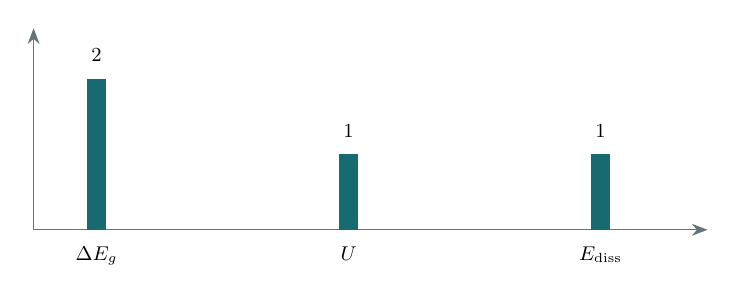
\begin{tikzpicture}[scale=.8,transform shape]
\draw[axis] (0,0)--(10.7,0);
\draw[axis] (0,0)--(0,3.2);
\draw[line width=7pt,color=accent] (1.0,0)--(1.0,2.400000000);
\node[below] at (1.0,-.14) {$\Delta E_g$};
\node[above] at (1.0,2.540000000) {$ 2 $};
\draw[line width=7pt,color=accent] (5.0,0)--(5.0,1.200000000);
\node[below] at (5.0,-.14) {$U$};
\node[above] at (5.0,1.340000000) {$ 1 $};
\draw[line width=7pt,color=accent] (9.0,0)--(9.0,1.200000000);
\node[below] at (9.0,-.14) {$E_{\rm diss}$};
\node[above] at (9.0,1.340000000) {$ 1 $};
\end{tikzpicture}
\figcaption{变图综三.3V6\quad 以$m^2g^2/(6K)$为单位的能量分配}
\end{minipage}\end{center}

\Needspace{20\baselineskip}
\item 测得悬挂杆的质量$m$和上下端线密度$\lambda_t,\lambda_b$，$\lambda_b>\lambda_t$，反求自然长度、劲度系数及实际总长。
\textbf{解：}变图综三.3V7下端无张力，故$\lambda_b=\lambda_0=m/L_0$，于是$L_0=m/\lambda_b$。上端$\lambda_t=\lambda_0/(1+\alpha)$，得$\alpha=\lambda_b/\lambda_t-1$。由$\alpha=mg/(KL_0)$求$K=g\lambda_b\lambda_t/(\lambda_b-\lambda_t)$，再由总长得$L=(m/2)(1/\lambda_b+1/\lambda_t)$。两个端点密度分别提供自然密度与最大伸长比，使材料长度和弹性刚度都可由静态量确定。
\begin{center}\begin{minipage}{.98\linewidth}\centering
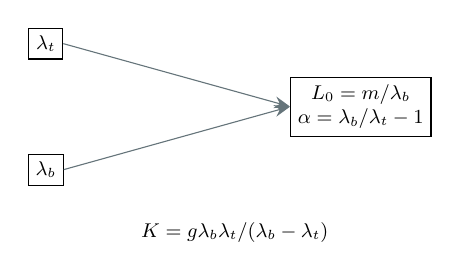
\begin{tikzpicture}[scale=.8,transform shape]
\node[draw] (t) at (0,1) {$\lambda_t$};\node[draw] (b) at (0,-1) {$\lambda_b$};\node[draw,align=center] (x) at (5,0) {$L_0=m/\lambda_b$\\$\alpha=\lambda_b/\lambda_t-1$};\draw[axis] (t.east)--(x.west);\draw[axis] (b.east)--(x.west);\node at (3,-2) {$K=g\lambda_b\lambda_t/(\lambda_b-\lambda_t)$};
\end{tikzpicture}
\figcaption{变图综三.3V7\quad 上下端密度分别确定自然密度和最大伸长比}
\end{minipage}\end{center}

\Needspace{20\baselineskip}
\item 改变材料质量分布为$\lambda_0(\xi)=(m/L_0)[1+\beta(2\xi/L_0-1)]$，$|\beta|<1$，轴向刚度仍为常量$KL_0$。求伸长和空间密度的参数表示。
\textbf{解：}变图综三.3V8令$u=\xi/L_0$，截面以下质量积分给$T=mg(1-u)(1+\beta u)$。局部伸长比$J=1+\alpha(1-u)(1+\beta u)$，从上端积分得$x/L_0=u+\alpha[u-u^2/2+\beta(u^2/2-u^3/3)]$，总伸长为$(mg/K)(1/2+\beta/6)$。质量守恒给$\lambda(x(u))=(m/L_0)[1+\beta(2u-1)]/J$。因$J>0$，该参数式对每个实际位置给唯一材料点；$\beta>0$时材料向下端集中，总伸长随之增加。
\begin{center}\begin{minipage}{.98\linewidth}\centering
\begin{tikzpicture}[scale=.8,transform shape]
\draw[axis] (0,0)--(10.7,0) node[right] {$x/L_0$};
\draw[axis] (0,0)--(0,3.2) node[above] {$\lambda/(m/L_0)$};\foreach \y/\lab in {0.45/{1/4},1.8/1,2.7/1.5}{\draw[thin] (0,\y)--(-.08,\y) node[left] {$\lab$};}
\node[above] at (5,3.5) {自然质量向下集中：$\alpha=1,\beta=1/2$};
\draw[traj] plot coordinates {(0.000000000,0.450000000) (0.105152900,0.458463091) (0.210082846,0.466978171) (0.314786184,0.475546470) (0.419259259,0.484169235) (0.523498416,0.492847740) (0.627500000,0.501583281) (0.731260356,0.510377176) (0.834775828,0.519230769) (0.938042763,0.528145431) (1.041057505,0.537122558) (1.143816399,0.546163571) (1.246315789,0.555269923) (1.348552022,0.564443092) (1.450521442,0.573684588) (1.552220395,0.582995951) (1.653645224,0.592378753) (1.754792276,0.601834597) (1.855657895,0.611365121) (1.956238426,0.620971997) (2.056530214,0.630656934) (2.156529605,0.640421677) (2.256232943,0.650268008) (2.355636574,0.660197750) (2.454736842,0.670212766) (2.553530093,0.680314961) (2.652012671,0.690506282) (2.750180921,0.700788723) (2.848031189,0.711164322) (2.945559820,0.721635166) (3.042763158,0.732203390) (3.139637549,0.742871180) (3.236179337,0.753640777) (3.332384868,0.764514472) (3.428250487,0.775494615) (3.523772539,0.786583613) (3.618947368,0.797783934) (3.713771321,0.809098106) (3.808240741,0.820528723) (3.902351974,0.832078445) (3.996101365,0.843750000) (4.089485258,0.855546187) (4.182500000,0.867469880) (4.275141935,0.879524026) (4.367407407,0.891711654) (4.459292763,0.904035874) (4.550794347,0.916499880) (4.641908504,0.929106953) (4.732631579,0.941860465) (4.822959917,0.954763884) (4.912889864,0.967820774) (5.002417763,0.981034800) (5.091539961,0.994409734) (5.180252802,1.007949454) (5.268552632,1.021657954) (5.356435794,1.035539343) (5.443898635,1.049597855) (5.530937500,1.063837848) (5.617548733,1.078263813) (5.703728679,1.092880376) (5.789473684,1.107692308) (5.874780093,1.122704525) (5.959644250,1.137922100) (6.044062500,1.153350264) (6.128031189,1.168994413) (6.211546662,1.184860121) (6.294605263,1.200953137) (6.377203338,1.217279404) (6.459337232,1.233845055) (6.541003289,1.250656433) (6.622197856,1.267720090) (6.702917276,1.285042803) (6.783157895,1.302631579) (6.862916058,1.320493668) (6.942188109,1.338636574) (7.020970395,1.357068063) (7.099259259,1.375796178) (7.177051048,1.394829252) (7.254342105,1.414175918) (7.331128777,1.433845125) (7.407407407,1.453846154) (7.483174342,1.474188630) (7.558425926,1.494882542) (7.633158504,1.515938259) (7.707368421,1.537366548) (7.781052022,1.559178594) (7.854205653,1.581386019) (7.926825658,1.604000909) (7.998908382,1.627035831) (8.070450171,1.650503859) (8.141447368,1.674418605) (8.211896321,1.698794239) (8.281793372,1.723645527) (8.351134868,1.748987854) (8.419917154,1.774837264) (8.488136574,1.801210491) (8.555789474,1.828125000) (8.622872198,1.855599026) (8.689381092,1.883651617) (8.755312500,1.912302681) (8.820662768,1.941573034) (8.885428241,1.971484453) (8.949605263,2.002059732) (9.013190180,2.033322746) (9.076179337,2.065298507) (9.138569079,2.098013245) (9.200355750,2.131494472) (9.261535697,2.165771067) (9.322105263,2.200873362) (9.382060794,2.236833236) (9.441398635,2.273684211) (9.500115132,2.311461560) (9.558206628,2.350202429) (9.615669469,2.389945956) (9.672500000,2.430733411) (9.728694566,2.472608340) (9.784249513,2.515616728) (9.839161184,2.559807171) (9.893425926,2.605231061) (9.947040083,2.651942796) (10.000000000,2.700000000)};
\node[below] at (0,-.12) {$0$};
\node[below] at (10,-.12) {$19/12$};
\end{tikzpicture}
\figcaption{变图综三.3V8\quad 自然质量向下集中：$\alpha=1,\beta=1/2$}
\end{minipage}\end{center}
\end{enumerate}

\Needspace{13\baselineskip}

\pdfbookmark[2]{第 4 题 阻尼振动、感应制动与受迫响应}{q4}

\section*{第 4 题\quad 阻尼振动、感应制动与受迫响应}\label{q:4}


（1）分别建立下列系统的运动方程，讨论能否振动及其条件。

甲：质量$m$、密度为水的$a$倍（$a>1$）的小球，用长$l$的轻质刚杆悬于水中，水对球的阻力为$-\gamma\boldsymbol v$。忽略杆的浮力、阻力，讨论小角度运动。

乙：间距$l$的水平平行导轨上有质量$m$的导体棒，与电阻$R$、自感$L$串联构成闭合回路。匀强磁场$B$垂直纸面向里。导轨和棒的电阻、摩擦忽略；初始棒向右以$v_0$运动，回路电流为零。分析速度和电流随时间的变化。

（2）对一般受迫振动方程
\[
\ddot x+2\beta\dot x+\omega_0^2x=h\cos pt
\]
（$\beta,\omega_0,h,p>0$），求完整解的结构和稳态振幅、相位，并说明暂态何时消失、振幅在何种频率达到最大。


\begin{center}\begin{minipage}{.98\linewidth}\centering
\begin{tikzpicture}[scale=.65,transform shape]

\draw[object] (-.7,0)--(.7,0);
\draw[guide] (0,0)--(0,-3.1);
\draw[object] (0,0)--(1.4,-2.4) node[midway,right] {$l$};
\fill[accent] (1.4,-2.4) circle (5pt) node[right] {$m$};
\draw[guide] (0,-.9) arc[start angle=-90,end angle=-59.74,radius=.9];
\node at (.45,-1.15) {$\theta$};
\draw[guide] (-1.5,-.8)--(2.7,-.8) node[right] {水面};

\begin{scope}[xshift=5.8cm]
\draw[object] (0,0)--(0,2)--(1.1,2);
\draw[object] (2.5,2)--(4,2)--(4,0)--(0,0);
\draw[object] (1.1,1.8) rectangle (2.5,2.2);
\node[above] at (1.8,2.2) {$L$};
\fill[white] (-.2,.5) rectangle (.2,1.5);
\draw[object] (-.2,.5) rectangle (.2,1.5);
\node[left] at (-.2,1) {$R$};
\draw[object,line width=2pt] (4,0)--(4,2);
\draw[motion] (4.2,1.3)--(5.3,1.3) node[right] {$v$};
\draw[motion] (3.7,.4)--(3.7,1.3) node[left] {$i$};
\node at (2,1) {$\otimes B$};
\draw[axis,<->] (5.8,0)--(5.8,2) node[midway,right] {$l$};
\end{scope}

\end{tikzpicture}
\figcaption{图综三.4\quad 水中轻杆摆与含串联电阻、自感的导体棒回路。}
\end{minipage}\end{center}

\Needspace{8\baselineskip}

\pdfbookmark[3]{题型定位}{q4-h0}

\subsection*{题型定位}

水中摆和含自感导体棒都先从具体受力、回路建立二阶方程，再与一般阻尼振动比较。受迫部分把初态齐次响应与驱动特解同时保留，按特征根给三种暂态，按实、虚投影给振幅相位。自由振荡条件与位移振幅峰的条件各由不同方程决定。

\Needspace{8\baselineskip}

\pdfbookmark[3]{知识点}{q4-h1}

\subsection*{知识点}

浮力降低有效恢复重力，黏滞阻力矩与角速度成正比，惯性质量保持为$m$。动生电动势、电感电流连续和安培力共同形成速度的二阶动力学；电阻耗散使机械能与电感能之和降低。齐次特征根决定欠、临界与过阻尼，初态由扣除特解后的两个常数表示。谐振特解的幅值由复动态刚度的模给出，相位取完整象限。位移峰值、速度峰值与自由衰减频率分别定义。

\Needspace{8\baselineskip}

\pdfbookmark[3]{物理图像}{q4-h2}

\subsection*{物理图像}

解图综三.4A给水中摆的重力、浮力和切向阻力，图B给逆时针电流与向左磁力。图C的速度曲线保留反向区间，三种阻尼都从零初始加速度出发。图D用同一比例尺画低、高频相位向量，图E显示不同阻尼的位移振幅随频率变化。图F在相同时间轴画完整受迫运动与周期特解，说明初始条件如何由暂态补足。

\Needspace{8\baselineskip}

\pdfbookmark[3]{解题入口}{q4-h3}

\subsection*{解题入口}

水中摆先对悬点列力矩，再作小角度近似，阻力矩中的$l^2$与惯性矩相消。导体棒保留$v,i$两个状态，以动生电动势和安培力方向写两方程；初态$i=0$给$\dot v=0$。一般受迫解先把正余弦系数列齐，求幅值和象限，再从完整初值扣除特解初值，再求齐次常数，最后对幅值分母求导找峰。

\Needspace{8\baselineskip}

\pdfbookmark[3]{标准解法}{q4-h4}

\subsection*{标准解法}


图综三.4中的轻杆可推可拉，摆球始终位于以悬点为圆心的圆周上。水的浮力为$mg/a$，因此重力与浮力的合力向下，大小$mg'=m(1-1/a)g$。
\begin{center}\begin{minipage}{.98\linewidth}\centering
\begin{tikzpicture}[scale=.85,transform shape]

\draw[object] (-.7,0)--(.7,0);
\draw[guide] (0,0)--(0,-3.1);
\draw[object] (0,0)--(1.4,-2.4) node[midway,right] {$l$};
\fill[accent] (1.4,-2.4) circle (5pt) node[right] {$m$};
\draw[guide] (0,-.9) arc[start angle=-90,end angle=-59.74,radius=.9];
\node at (.45,-1.15) {$\theta$};
\draw[guide] (-1.5,-.8)--(2.7,-.8) node[right] {水面};

\draw[force] (1.4,-2.4)--(1.4,-4) node[below] {$mg$};
\draw[force,color=warm] (1.65,-2.4)--(1.65,-1.25) node[right] {$mg/a$};
\draw[motion] (1.3,-2.5)--(.3,-3.08) node[below left] {$-\gamma\boldsymbol v$};
\node[align=left] at (5,-2) {$g'=(1-1/a)g$\\$\beta_1=\gamma/(2m)$\\$\omega_1^2=g'/l$};

\end{tikzpicture}
\figcaption{解图综三.4A\quad 重力、浮力及切向阻力；恢复力用有效重力，惯性仍用m。}
\end{minipage}\end{center}
密度比$a$使排开水的质量为$m/a$，所以浮力为$mg/a$。两力都沿竖直方向，它们关于悬点的力矩之差以同一个力臂$l\sin\theta$计算；球本身绕悬点的转动惯量仍是$ml^2$。

解图综三.4A以偏离竖直向下方向的$\theta$为坐标。阻力沿切线反向，大小$\gamma l|\dot\theta|$。关于悬点列力矩方程：
\[
ml^2\ddot\theta=-mg'l\sin\theta-\gamma l^2\dot\theta.
\]
小角度近似$\sin\theta\simeq\theta$，得到
\[
\ddot\theta+\frac{\gamma}{m}\dot\theta+\frac{g'}l\theta=0.
\]
阻力矩是阻力乘杆长，速度又等于$l\dot\theta$，所以阻力矩含$l^2$；除以惯性矩$ml^2$后阻尼率为$\gamma/m$。恢复力矩只含一个$l$，除后为$g'/l$，杆越长恢复频率越低。记$\beta_1=\gamma/(2m)$、$\omega_1=\sqrt{g'/l}$。特征根为
$-\beta_1\pm\sqrt{\beta_1^2-\omega_1^2}$。只有$\beta_1<\omega_1$时有衰减的正弦运动：
\[
\theta=e^{-\beta_1t}(C\cos\Omega_1t+D\sin\Omega_1t),\quad
\Omega_1=\sqrt{\omega_1^2-\beta_1^2}.
\]
故振动条件为
\[
\boxed{\gamma<2m\sqrt{\frac{(1-1/a)g}{l}}}
\quad\Longleftrightarrow\quad
\boxed{l<\frac{4m^2(1-1/a)g}{\gamma^2}}.
\]
等号为临界阻尼，大于临界值为过阻尼，均无往复的正弦振荡。浮力只改变恢复力，阻力项仍含小球本身的惯性质量$m$。
\begin{center}\begin{minipage}{.98\linewidth}\centering
\begin{tikzpicture}[scale=.85,transform shape]

\draw[object] (0,0)--(0,2)--(1.1,2);
\draw[object] (2.5,2)--(4,2)--(4,0)--(0,0);
\draw[object] (1.1,1.8) rectangle (2.5,2.2);
\node[above] at (1.8,2.2) {$L$};
\fill[white] (-.2,.5) rectangle (.2,1.5);
\draw[object] (-.2,.5) rectangle (.2,1.5);
\node[left] at (-.2,1) {$R$};
\draw[object,line width=2pt] (4,0)--(4,2);
\draw[motion] (4.2,1.3)--(5.3,1.3) node[right] {$v$};
\draw[motion] (3.7,.4)--(3.7,1.3) node[left] {$i$};
\node at (2,1) {$\otimes B$};
\draw[axis,<->] (5.8,0)--(5.8,2) node[midway,right] {$l$};

\draw[force] (3.8,.5)--(2.7,.5) node[midway,below] {$Bli$};
\node at (2.5,-1) {$L\dot i+Ri=Blv,\qquad m\dot v=-Bli$};
\node at (2.5,-2) {逆时针为正电流，初始$i=0$};

\end{tikzpicture}
\figcaption{解图综三.4B\quad 回路正向与棒的磁力；电感允许能量先储存再返回机械运动。}
\end{minipage}\end{center}
解图综三.4B将逆时针电流$i$定为正：右侧棒内正电流向上，所受磁力向左。运动电动势使这一方向的电流增大，回路和棒分别满足
\[
L\dot i+Ri=Blv,\qquad m\dot v=-Bli.
\]
由机械方程先得$i=-m\dot v/(Bl)$，再对时间求导得到$\dot i=-m\ddot v/(Bl)$。代入回路式后，$-Lm\ddot v/(Bl)-Rm\dot v/(Bl)=Blv$，乘$-Bl/(mL)$并移项，消去$i$，得到
\[
\boxed{\ddot v+\frac RL\dot v+\frac{B^2l^2}{mL}v=0},\qquad
v(0)=v_0,\quad\dot v(0)=0.
\]
两个一阶状态分别记录棒的机械运动和电感储能，初态$v_0,0$给$\dot i(0)=Blv_0/L$、$\dot v(0)=0$。电流先从零增长，随后磁力才逐渐制动棒。自感使电流不能瞬时跳变，故初始磁力与初始加速度均为零。令
$\beta_2=R/(2L)$、$\omega_2=Bl/\sqrt{mL}$，临界电阻为
\[
\boxed{R_c=2Bl\sqrt{L/m}}.
\]
在$0<R<R_c$时，$\Omega_2=\sqrt{\omega_2^2-\beta_2^2}$，
\[
\boxed{v=v_0e^{-\beta_2t}
\left(\cos\Omega_2t+\frac{\beta_2}{\Omega_2}\sin\Omega_2t\right)},\qquad
\boxed{i=\frac{Blv_0}{L\Omega_2}e^{-\beta_2t}\sin\Omega_2t}.
\]
欠阻尼速度表达式中的余弦、正弦系数由$v(0)=v_0,\dot v(0)=0$确定，电流则由$-m\dot v/(Bl)$求出，求导时两个余弦项相消，只留下正弦项。速度过零后，电感中的原方向电流还可持续一段时间。棒可反向运动，磁场能在机械能与电感能之间交换。在$R=R_c$时
\[
v=v_0(1+\beta_2t)e^{-\beta_2t},\qquad
i=\frac{Blv_0}{L}t e^{-\beta_2t}.
\]
在$R>R_c$时，令$q=\sqrt{\beta_2^2-\omega_2^2}$，则
\[
v=v_0e^{-\beta_2t}
\left(\cosh qt+\frac{\beta_2}{q}\sinh qt\right),\qquad
i=\frac{Blv_0}{Lq}e^{-\beta_2t}\sinh qt.
\]
\begin{center}\begin{minipage}{.98\linewidth}\centering
\begin{tikzpicture}[scale=.8,transform shape]
\draw[axis] (0,0)--(10.7,0) node[right] {$\omega_2t$};
\draw[axis] (0,0)--(0,3.2) node[above] {$v/v_0$};\foreach \y/\lab in {0.38/-.2,2.66/1}{\draw[thin] (0,\y)--(-.08,\y) node[left] {$\lab$};}
\node[above] at (5,3.5) {实线欠阻尼，细线临界，虚线过阻尼；各曲线初始斜率为零};
\draw[traj] plot coordinates {(0.000000000,2.660000000) (0.062500000,2.657649062) (0.125000000,2.650694911) (0.187500000,2.639290716) (0.250000000,2.623596078) (0.312500000,2.603776443) (0.375000000,2.580002527) (0.437500000,2.552449737) (0.500000000,2.521297599) (0.562500000,2.486729200) (0.625000000,2.448930623) (0.687500000,2.408090409) (0.750000000,2.364399016) (0.812500000,2.318048292) (0.875000000,2.269230964) (0.937500000,2.218140138) (1.000000000,2.164968809) (1.062500000,2.109909392) (1.125000000,2.053153265) (1.187500000,1.994890328) (1.250000000,1.935308577) (1.312500000,1.874593701) (1.375000000,1.812928691) (1.437500000,1.750493469) (1.500000000,1.687464536) (1.562500000,1.624014639) (1.625000000,1.560312455) (1.687500000,1.496522298) (1.750000000,1.432803843) (1.812500000,1.369311868) (1.875000000,1.306196020) (1.937500000,1.243600597) (2.000000000,1.181664349) (2.062500000,1.120520305) (2.125000000,1.060295611) (2.187500000,1.001111389) (2.250000000,0.943082623) (2.312500000,0.886318050) (2.375000000,0.830920084) (2.437500000,0.776984745) (2.500000000,0.724601613) (2.562500000,0.673853800) (2.625000000,0.624817935) (2.687500000,0.577564165) (2.750000000,0.532156177) (2.812500000,0.488651232) (2.875000000,0.447100211) (2.937500000,0.407547679) (3.000000000,0.370031966) (3.062500000,0.334585251) (3.125000000,0.301233668) (3.187500000,0.269997421) (3.250000000,0.240890907) (3.312500000,0.213922854) (3.375000000,0.189096465) (3.437500000,0.166409577) (3.500000000,0.145854820) (3.562500000,0.127419794) (3.625000000,0.111087245) (3.687500000,0.096835252) (3.750000000,0.084637418) (3.812500000,0.074463071) (3.875000000,0.066277459) (3.937500000,0.060041963) (4.000000000,0.055714301) (4.062500000,0.053248745) (4.125000000,0.052596333) (4.187500000,0.053705085) (4.250000000,0.056520220) (4.312500000,0.060984375) (4.375000000,0.067037821) (4.437500000,0.074618684) (4.500000000,0.083663152) (4.562500000,0.094105701) (4.625000000,0.105879296) (4.687500000,0.118915609) (4.750000000,0.133145221) (4.812500000,0.148497826) (4.875000000,0.164902431) (4.937500000,0.182287551) (5.000000000,0.200581398) (5.062500000,0.219712070) (5.125000000,0.239607728) (5.187500000,0.260196773) (5.250000000,0.281408014) (5.312500000,0.303170835) (5.375000000,0.325415344) (5.437500000,0.348072532) (5.500000000,0.371074412) (5.562500000,0.394354159) (5.625000000,0.417846236) (5.687500000,0.441486523) (5.750000000,0.465212429) (5.812500000,0.488963001) (5.875000000,0.512679028) (5.937500000,0.536303133) (6.000000000,0.559779863) (6.062500000,0.583055764) (6.125000000,0.606079459) (6.187500000,0.628801708) (6.250000000,0.651175471) (6.312500000,0.673155954) (6.375000000,0.694700657) (6.437500000,0.715769408) (6.500000000,0.736324396) (6.562500000,0.756330189) (6.625000000,0.775753758) (6.687500000,0.794564482) (6.750000000,0.812734156) (6.812500000,0.830236984) (6.875000000,0.847049576) (6.937500000,0.863150934) (7.000000000,0.878522431) (7.062500000,0.893147786) (7.125000000,0.907013039) (7.187500000,0.920106513) (7.250000000,0.932418776) (7.312500000,0.943942600) (7.375000000,0.954672911) (7.437500000,0.964606739) (7.500000000,0.973743162) (7.562500000,0.982083251) (7.625000000,0.989630005) (7.687500000,0.996388286) (7.750000000,1.002364757) (7.812500000,1.007567808) (7.875000000,1.012007484) (7.937500000,1.015695416) (8.000000000,1.018644738) (8.062500000,1.020870019) (8.125000000,1.022387177) (8.187500000,1.023213404) (8.250000000,1.023367087) (8.312500000,1.022867724) (8.375000000,1.021735844) (8.437500000,1.019992929) (8.500000000,1.017661329) (8.562500000,1.014764183) (8.625000000,1.011325340) (8.687500000,1.007369277) (8.750000000,1.002921021) (8.812500000,0.998006072) (8.875000000,0.992650325) (8.937500000,0.986879996) (9.000000000,0.980721546) (9.062500000,0.974201610) (9.125000000,0.967346926) (9.187500000,0.960184266) (9.250000000,0.952740369) (9.312500000,0.945041876) (9.375000000,0.937115268) (9.437500000,0.928986806) (9.500000000,0.920682470) (9.562500000,0.912227906) (9.625000000,0.903648373) (9.687500000,0.894968689) (9.750000000,0.886213187) (9.812500000,0.877405667) (9.875000000,0.868569354) (9.937500000,0.859726857) (10.000000000,0.850900131)};
\draw[thin,color=black] plot coordinates {(0.000000000,2.660000000) (0.062500000,2.657702702) (0.125000000,2.651110204) (0.187500000,2.640646928) (0.250000000,2.626706117) (0.312500000,2.609651860) (0.375000000,2.589821005) (0.437500000,2.567524950) (0.500000000,2.543051322) (0.562500000,2.516665558) (0.625000000,2.488612380) (0.687500000,2.459117192) (0.750000000,2.428387374) (0.812500000,2.396613510) (0.875000000,2.363970531) (0.937500000,2.330618788) (1.000000000,2.296705057) (1.062500000,2.262363486) (1.125000000,2.227716472) (1.187500000,2.192875492) (1.250000000,2.157941876) (1.312500000,2.123007533) (1.375000000,2.088155624) (1.437500000,2.053461203) (1.500000000,2.018991806) (1.562500000,1.984808007) (1.625000000,1.950963936) (1.687500000,1.917507764) (1.750000000,1.884482156) (1.812500000,1.851924691) (1.875000000,1.819868261) (1.937500000,1.788341433) (2.000000000,1.757368799) (2.062500000,1.726971290) (2.125000000,1.697166478) (2.187500000,1.667968855) (2.250000000,1.639390085) (2.312500000,1.611439256) (2.375000000,1.584123092) (2.437500000,1.557446171) (2.500000000,1.531411114) (2.562500000,1.506018766) (2.625000000,1.481268362) (2.687500000,1.457157684) (2.750000000,1.433683203) (2.812500000,1.410840212) (2.875000000,1.388622950) (2.937500000,1.367024718) (3.000000000,1.346037978) (3.062500000,1.325654460) (3.125000000,1.305865241) (3.187500000,1.286660837) (3.250000000,1.268031275) (3.312500000,1.249966163) (3.375000000,1.232454755) (3.437500000,1.215486011) (3.500000000,1.199048652) (3.562500000,1.183131207) (3.625000000,1.167722061) (3.687500000,1.152809493) (3.750000000,1.138381720) (3.812500000,1.124426923) (3.875000000,1.110933287) (3.937500000,1.097889020) (4.000000000,1.085282388) (4.062500000,1.073101728) (4.125000000,1.061335478) (4.187500000,1.049972187) (4.250000000,1.039000537) (4.312500000,1.028409356) (4.375000000,1.018187628) (4.437500000,1.008324510) (4.500000000,0.998809334) (4.562500000,0.989631623) (4.625000000,0.980781091) (4.687500000,0.972247656) (4.750000000,0.964021439) (4.812500000,0.956092771) (4.875000000,0.948452196) (4.937500000,0.941090470) (5.000000000,0.933998569) (5.062500000,0.927167685) (5.125000000,0.920589225) (5.187500000,0.914254815) (5.250000000,0.908156299) (5.312500000,0.902285733) (5.375000000,0.896635389) (5.437500000,0.891197750) (5.500000000,0.885965507) (5.562500000,0.880931561) (5.625000000,0.876089014) (5.687500000,0.871431170) (5.750000000,0.866951532) (5.812500000,0.862643797) (5.875000000,0.858501851) (5.937500000,0.854519770) (6.000000000,0.850691812) (6.062500000,0.847012416) (6.125000000,0.843476196) (6.187500000,0.840077938) (6.250000000,0.836812596) (6.312500000,0.833675288) (6.375000000,0.830661293) (6.437500000,0.827766044) (6.500000000,0.824985129) (6.562500000,0.822314281) (6.625000000,0.819749379) (6.687500000,0.817286442) (6.750000000,0.814921624) (6.812500000,0.812651214) (6.875000000,0.810471627) (6.937500000,0.808379405) (7.000000000,0.806371211) (7.062500000,0.804443824) (7.125000000,0.802594140) (7.187500000,0.800819164) (7.250000000,0.799116007) (7.312500000,0.797481888) (7.375000000,0.795914122) (7.437500000,0.794410124) (7.500000000,0.792967404) (7.562500000,0.791583562) (7.625000000,0.790256286) (7.687500000,0.788983350) (7.750000000,0.787762611) (7.812500000,0.786592006) (7.875000000,0.785469547) (7.937500000,0.784393324) (8.000000000,0.783361495) (8.062500000,0.782372291) (8.125000000,0.781424008) (8.187500000,0.780515008) (8.250000000,0.779643714) (8.312500000,0.778808611) (8.375000000,0.778008241) (8.437500000,0.777241202) (8.500000000,0.776506148) (8.562500000,0.775801782) (8.625000000,0.775126859) (8.687500000,0.774480184) (8.750000000,0.773860606) (8.812500000,0.773267020) (8.875000000,0.772698365) (8.937500000,0.772153620) (9.000000000,0.771631807) (9.062500000,0.771131984) (9.125000000,0.770653246) (9.187500000,0.770194728) (9.250000000,0.769755594) (9.312500000,0.769335045) (9.375000000,0.768932313) (9.437500000,0.768546659) (9.500000000,0.768177376) (9.562500000,0.767823785) (9.625000000,0.767485233) (9.687500000,0.767161095) (9.750000000,0.766850769) (9.812500000,0.766553679) (9.875000000,0.766269273) (9.937500000,0.765997020) (10.000000000,0.765736411)};
\draw[dashed,thick,color=warm] plot coordinates {(0.000000000,2.660000000) (0.062500000,2.657739893) (0.125000000,2.651389852) (0.187500000,2.641534309) (0.250000000,2.628684430) (0.312500000,2.613287125) (0.375000000,2.595732970) (0.437500000,2.576363140) (0.500000000,2.555475502) (0.562500000,2.533329957) (0.625000000,2.510153121) (0.687500000,2.486142441) (0.750000000,2.461469793) (0.812500000,2.436284652) (0.875000000,2.410716858) (0.937500000,2.384879058) (1.000000000,2.358868831) (1.062500000,2.332770566) (1.125000000,2.306657102) (1.187500000,2.280591166) (1.250000000,2.254626639) (1.312500000,2.228809659) (1.375000000,2.203179598) (1.437500000,2.177769907) (1.500000000,2.152608869) (1.562500000,2.127720247) (1.625000000,2.103123864) (1.687500000,2.078836103) (1.750000000,2.054870348) (1.812500000,2.031237373) (1.875000000,2.007945677) (1.937500000,1.985001783) (2.000000000,1.962410501) (2.062500000,1.940175148) (2.125000000,1.918297757) (2.187500000,1.896779244) (2.250000000,1.875619567) (2.312500000,1.854817855) (2.375000000,1.834372529) (2.437500000,1.814281400) (2.500000000,1.794541765) (2.562500000,1.775150481) (2.625000000,1.756104032) (2.687500000,1.737398595) (2.750000000,1.719030084) (2.812500000,1.700994203) (2.875000000,1.683286482) (2.937500000,1.665902310) (3.000000000,1.648836971) (3.062500000,1.632085661) (3.125000000,1.615643521) (3.187500000,1.599505648) (3.250000000,1.583667117) (3.312500000,1.568122995) (3.375000000,1.552868350) (3.437500000,1.537898269) (3.500000000,1.523207859) (3.562500000,1.508792263) (3.625000000,1.494646659) (3.687500000,1.480766274) (3.750000000,1.467146381) (3.812500000,1.453782307) (3.875000000,1.440669440) (3.937500000,1.427803221) (4.000000000,1.415179160) (4.062500000,1.402792826) (4.125000000,1.390639855) (4.187500000,1.378715949) (4.250000000,1.367016877) (4.312500000,1.355538476) (4.375000000,1.344276650) (4.437500000,1.333227371) (4.500000000,1.322386679) (4.562500000,1.311750681) (4.625000000,1.301315551) (4.687500000,1.291077532) (4.750000000,1.281032929) (4.812500000,1.271178115) (4.875000000,1.261509529) (4.937500000,1.252023670) (5.000000000,1.242717104) (5.062500000,1.233586458) (5.125000000,1.224628420) (5.187500000,1.215839740) (5.250000000,1.207217225) (5.312500000,1.198757745) (5.375000000,1.190458223) (5.437500000,1.182315644) (5.500000000,1.174327045) (5.562500000,1.166489521) (5.625000000,1.158800218) (5.687500000,1.151256339) (5.750000000,1.143855136) (5.812500000,1.136593914) (5.875000000,1.129470030) (5.937500000,1.122480887) (6.000000000,1.115623940) (6.062500000,1.108896689) (6.125000000,1.102296684) (6.187500000,1.095821520) (6.250000000,1.089468835) (6.312500000,1.083236316) (6.375000000,1.077121688) (6.437500000,1.071122724) (6.500000000,1.065237237) (6.562500000,1.059463080) (6.625000000,1.053798148) (6.687500000,1.048240375) (6.750000000,1.042787736) (6.812500000,1.037438241) (6.875000000,1.032189940) (6.937500000,1.027040919) (7.000000000,1.021989300) (7.062500000,1.017033241) (7.125000000,1.012170935) (7.187500000,1.007400607) (7.250000000,1.002720519) (7.312500000,0.998128963) (7.375000000,0.993624265) (7.437500000,0.989204782) (7.500000000,0.984868902) (7.562500000,0.980615043) (7.625000000,0.976441654) (7.687500000,0.972347213) (7.750000000,0.968330227) (7.812500000,0.964389230) (7.875000000,0.960522784) (7.937500000,0.956729480) (8.000000000,0.953007934) (8.062500000,0.949356789) (8.125000000,0.945774712) (8.187500000,0.942260398) (8.250000000,0.938812564) (8.312500000,0.935429953) (8.375000000,0.932111331) (8.437500000,0.928855487) (8.500000000,0.925661234) (8.562500000,0.922527408) (8.625000000,0.919452864) (8.687500000,0.916436481) (8.750000000,0.913477159) (8.812500000,0.910573820) (8.875000000,0.907725402) (8.937500000,0.904930869) (9.000000000,0.902189200) (9.062500000,0.899499395) (9.125000000,0.896860473) (9.187500000,0.894271473) (9.250000000,0.891731448) (9.312500000,0.889239473) (9.375000000,0.886794640) (9.437500000,0.884396055) (9.500000000,0.882042844) (9.562500000,0.879734150) (9.625000000,0.877469129) (9.687500000,0.875246956) (9.750000000,0.873066820) (9.812500000,0.870927925) (9.875000000,0.868829492) (9.937500000,0.866770756) (10.000000000,0.864750965)};
\node[below] at (0,-.12) {$0$};
\node[below] at (5,-.12) {$4$};
\node[below] at (10,-.12) {$8$};
\draw[dotted] (0,.76)--(10,.76);\node[left] at (0,.76) {$0$};
\end{tikzpicture}
\figcaption{解图综三.4C\quad 实线欠阻尼，细线临界，虚线过阻尼；各曲线初始斜率为零}
\end{minipage}\end{center}
解图综三.4C比较三种阻尼。将力学方程乘$v$、回路方程乘$i$并相加，
\[
\frac d{dt}\left(\frac12mv^2+\frac12Li^2\right)=-Ri^2.
\]
这一步的耦合功率$Blvi$在两式中一正一负，表示机械能与磁能之间的交换；相加后只剩电阻热耗散。对$R>0$，最终$v,i\to0$；从动力学方程积分得
$\int_0^\infty i\,dt=mv_0/(Bl)$，再积分回路方程，左端电感项为$L[i(\infty)-i(0)]=0$，因此$Bl\Delta x=R\int_0^\infty i\,\mathrm dt$。把前式的电流积分代入，便有
\[
\boxed{\Delta x=\int_0^\infty v\,dt=\frac{Rm v_0}{B^2l^2}}.
\]
这里速度按方向带符号积分，得到净位移；总路程使用$|v|$的积分。若$R=0$，系统不衰减，
$v=v_0\cos\omega_2t$，$i=Blv_0\sin\omega_2t/(L\omega_2)$；
零电阻下位移随时间周期变化，前述净位移积分用于$R>0$的衰减过程。

水中摆和导体棒分别使用角度与速度作振子变量，它们的特征方程结构相同，但变量代表的物理对象不同。以下用一般位移坐标$x$讨论外力驱动，令$h$为驱动力幅值除以质量。

一般受迫方程的解等于一个特解加齐次解。先令
$x_s=A\cos(pt-\delta)$，代入后分别比较$\cos pt,\sin pt$的系数：
\[
A[(\omega_0^2-p^2)\cos\delta+2\beta p\sin\delta]=h,
\]
\[
A[(\omega_0^2-p^2)\sin\delta-2\beta p\cos\delta]=0.
\]
将两式分别平方再相加时，含$\sin\delta\cos\delta$的交叉项相消，留下$A^2[(\omega_0^2-p^2)^2+4\beta^2p^2]=h^2$。同时由两方程得到$\cos\delta=(\omega_0^2-p^2)/D$、$\sin\delta=2\beta p/D$，$D$为分母的正平方根。由$A>0$取正振幅，并按图D中的两分量确定相位，得到
\[
\boxed{A=\frac{h}{\sqrt{(\omega_0^2-p^2)^2+4\beta^2p^2}}},
\quad
\boxed{\delta=\operatorname{atan2}(2\beta p,\omega_0^2-p^2)\in(0,\pi)}.
\]
\begin{center}\begin{minipage}{.98\linewidth}\centering
\begin{tikzpicture}[scale=.8,transform shape]
\draw[axis] (-2.5,0)--(2.4,0) node[right] {$\omega_0^2-p^2$};\draw[axis] (0,-.3)--(0,2.6) node[above] {$2\beta p$};\draw[motion] (0,0)--(1.125,.45) node[above right] {低频};\draw[force] (0,0)--(-1.875,1.35) node[above left] {高频};\draw (.65,0) arc(0:144.246113:.65);\node at (-.6,.9) {$\delta$};\node[align=left] at (1,-1.2) {相同坐标比例\qquad $0<\delta<\pi$};
\end{tikzpicture}
\figcaption{解图综三.4D\quad 动态刚度的两个相位示例，位移滞后角按矢量象限确定}
\end{minipage}\end{center}
解图综三.4D中的相位向量横分量为$\omega_0^2-p^2$，纵分量为$2\beta p>0$。
低频时$\delta<\pi/2$，$p=\omega_0$时$\delta=\pi/2$，高频时$\delta>\pi/2$。
相位按两分量的符号进入相应象限。

\begin{center}\begin{minipage}{.98\linewidth}\centering
\begin{tikzpicture}[scale=.8,transform shape]
\draw[axis] (0,0)--(10.7,0) node[right] {$\omega_0t$};
\draw[axis] (0,0)--(0,3.2) node[above] {$x\omega_0^2/h$};\foreach \y/\lab in {0.56/-1,2.16/1,2.96/2}{\draw[thin] (0,\y)--(-.08,\y) node[left] {$\lab$};}
\node[above] at (5,3.5) {取$\beta/\omega_0=.3,p/\omega_0=1.2$；实线完整运动，虚线周期特解};
\draw[traj] plot coordinates {(0.000000000,1.360000000) (0.041666667,1.361541923) (0.083333333,1.366077212) (0.125000000,1.373452460) (0.166666667,1.383491987) (0.208333333,1.395999570) (0.250000000,1.410760291) (0.291666667,1.427542471) (0.333333333,1.446099701) (0.375000000,1.466172927) (0.416666667,1.487492601) (0.458333333,1.509780870) (0.500000000,1.532753789) (0.541666667,1.556123552) (0.583333333,1.579600716) (0.625000000,1.602896414) (0.666666667,1.625724536) (0.708333333,1.647803868) (0.750000000,1.668860179) (0.791666667,1.688628229) (0.833333333,1.706853711) (0.875000000,1.723295091) (0.916666667,1.737725346) (0.958333333,1.749933593) (1.000000000,1.759726596) (1.041666667,1.766930139) (1.083333333,1.771390258) (1.125000000,1.772974339) (1.166666667,1.771572052) (1.208333333,1.767096138) (1.250000000,1.759483033) (1.291666667,1.748693326) (1.333333333,1.734712062) (1.375000000,1.717548866) (1.416666667,1.697237916) (1.458333333,1.673837739) (1.500000000,1.647430853) (1.541666667,1.618123248) (1.583333333,1.586043709) (1.625000000,1.551342991) (1.666666667,1.514192855) (1.708333333,1.474784953) (1.750000000,1.433329599) (1.791666667,1.390054403) (1.833333333,1.345202805) (1.875000000,1.299032496) (1.916666667,1.251813754) (1.958333333,1.203827685) (2.000000000,1.155364413) (2.041666667,1.106721184) (2.083333333,1.058200450) (2.125000000,1.010107892) (2.166666667,0.962750438) (2.208333333,0.916434260) (2.250000000,0.871462777) (2.291666667,0.828134666) (2.333333333,0.786741910) (2.375000000,0.747567871) (2.416666667,0.710885425) (2.458333333,0.676955146) (2.500000000,0.646023577) (2.541666667,0.618321574) (2.583333333,0.594062745) (2.625000000,0.573441997) (2.666666667,0.556634189) (2.708333333,0.543792909) (2.750000000,0.535049379) (2.791666667,0.530511491) (2.833333333,0.530262990) (2.875000000,0.534362792) (2.916666667,0.542844466) (2.958333333,0.555715856) (3.000000000,0.572958865) (3.041666667,0.594529398) (3.083333333,0.620357456) (3.125000000,0.650347394) (3.166666667,0.684378328) (3.208333333,0.722304704) (3.250000000,0.763957008) (3.291666667,0.809142631) (3.333333333,0.857646870) (3.375000000,0.909234065) (3.416666667,0.963648870) (3.458333333,1.020617639) (3.500000000,1.079849930) (3.541666667,1.141040115) (3.583333333,1.203869082) (3.625000000,1.268006025) (3.666666667,1.333110310) (3.708333333,1.398833403) (3.750000000,1.464820856) (3.791666667,1.530714329) (3.833333333,1.596153646) (3.875000000,1.660778866) (3.916666667,1.724232365) (3.958333333,1.786160903) (4.000000000,1.846217683) (4.041666667,1.904064369) (4.083333333,1.959373071) (4.125000000,2.011828269) (4.166666667,2.061128673) (4.208333333,2.106989012) (4.250000000,2.149141730) (4.291666667,2.187338587) (4.333333333,2.221352156) (4.375000000,2.250977199) (4.416666667,2.276031927) (4.458333333,2.296359126) (4.500000000,2.311827141) (4.541666667,2.322330726) (4.583333333,2.327791731) (4.625000000,2.328159655) (4.666666667,2.323412022) (4.708333333,2.313554615) (4.750000000,2.298621539) (4.791666667,2.278675125) (4.833333333,2.253805676) (4.875000000,2.224131052) (4.916666667,2.189796092) (4.958333333,2.150971888) (5.000000000,2.107854904) (5.041666667,2.060665954) (5.083333333,2.009649030) (5.125000000,1.955070004) (5.166666667,1.897215202) (5.208333333,1.836389854) (5.250000000,1.772916439) (5.291666667,1.707132925) (5.333333333,1.639390921) (5.375000000,1.570053745) (5.416666667,1.499494422) (5.458333333,1.428093625) (5.500000000,1.356237569) (5.541666667,1.284315865) (5.583333333,1.212719355) (5.625000000,1.141837938) (5.666666667,1.072058388) (5.708333333,1.003762194) (5.750000000,0.937323425) (5.791666667,0.873106630) (5.833333333,0.811464787) (5.875000000,0.752737316) (5.916666667,0.697248166) (5.958333333,0.645303984) (6.000000000,0.597192375) (6.041666667,0.553180271) (6.083333333,0.513512415) (6.125000000,0.478409957) (6.166666667,0.448069193) (6.208333333,0.422660431) (6.250000000,0.402327011) (6.291666667,0.387184463) (6.333333333,0.377319832) (6.375000000,0.372791150) (6.416666667,0.373627082) (6.458333333,0.379826721) (6.500000000,0.391359564) (6.541666667,0.408165645) (6.583333333,0.430155829) (6.625000000,0.457212282) (6.666666667,0.489189090) (6.708333333,0.525913043) (6.750000000,0.567184569) (6.791666667,0.612778818) (6.833333333,0.662446887) (6.875000000,0.715917185) (6.916666667,0.772896918) (6.958333333,0.833073700) (7.000000000,0.896117278) (7.041666667,0.961681348) (7.083333333,1.029405471) (7.125000000,1.098917066) (7.166666667,1.169833476) (7.208333333,1.241764085) (7.250000000,1.314312487) (7.291666667,1.387078691) (7.333333333,1.459661335) (7.375000000,1.531659929) (7.416666667,1.602677074) (7.458333333,1.672320682) (7.500000000,1.740206155) (7.541666667,1.805958534) (7.583333333,1.869214587) (7.625000000,1.929624838) (7.666666667,1.986855518) (7.708333333,2.040590431) (7.750000000,2.090532718) (7.791666667,2.136406522) (7.833333333,2.177958530) (7.875000000,2.214959390) (7.916666667,2.247205001) (7.958333333,2.274517652) (8.000000000,2.296747025) (8.041666667,2.313771038) (8.083333333,2.325496535) (8.125000000,2.331859809) (8.166666667,2.332826967) (8.208333333,2.328394124) (8.250000000,2.318587434) (8.291666667,2.303462945) (8.333333333,2.283106299) (8.375000000,2.257632252) (8.416666667,2.227184043) (8.458333333,2.191932601) (8.500000000,2.152075590) (8.541666667,2.107836313) (8.583333333,2.059462469) (8.625000000,2.007224773) (8.666666667,1.951415444) (8.708333333,1.892346582) (8.750000000,1.830348422) (8.791666667,1.765767492) (8.833333333,1.698964682) (8.875000000,1.630313228) (8.916666667,1.560196625) (8.958333333,1.489006489) (9.000000000,1.417140368) (9.041666667,1.344999523) (9.083333333,1.272986680) (9.125000000,1.201503789) (9.166666667,1.130949768) (9.208333333,1.061718280) (9.250000000,0.994195529) (9.291666667,0.928758104) (9.333333333,0.865770869) (9.375000000,0.805584930) (9.416666667,0.748535666) (9.458333333,0.694940856) (9.500000000,0.645098903) (9.541666667,0.599287166) (9.583333333,0.557760410) (9.625000000,0.520749377) (9.666666667,0.488459506) (9.708333333,0.461069775) (9.750000000,0.438731709) (9.791666667,0.421568529) (9.833333333,0.409674467) (9.875000000,0.403114243) (9.916666667,0.401922699) (9.958333333,0.406104614) (10.000000000,0.415634676)};
\draw[dashed,thick,color=warm] plot coordinates {(0.000000000,0.865617978) (0.041666667,0.927625067) (0.083333333,0.992063125) (0.125000000,1.058569858) (0.166666667,1.126771341) (0.208333333,1.196284121) (0.250000000,1.266717370) (0.291666667,1.337675089) (0.333333333,1.408758326) (0.375000000,1.479567426) (0.416666667,1.549704275) (0.458333333,1.618774537) (0.500000000,1.686389875) (0.541666667,1.752170130) (0.583333333,1.815745462) (0.625000000,1.876758427) (0.666666667,1.934865989) (0.708333333,1.989741444) (0.750000000,2.041076264) (0.791666667,2.088581826) (0.833333333,2.131991036) (0.875000000,2.171059831) (0.916666667,2.205568552) (0.958333333,2.235323180) (1.000000000,2.260156422) (1.041666667,2.279928658) (1.083333333,2.294528720) (1.125000000,2.303874521) (1.166666667,2.307913517) (1.208333333,2.306622998) (1.250000000,2.300010220) (1.291666667,2.288112363) (1.333333333,2.270996320) (1.375000000,2.248758325) (1.416666667,2.221523407) (1.458333333,2.189444691) (1.500000000,2.152702535) (1.541666667,2.111503517) (1.583333333,2.066079273) (1.625000000,2.016685195) (1.666666667,1.963598994) (1.708333333,1.907119139) (1.750000000,1.847563182) (1.791666667,1.785265967) (1.833333333,1.720577752) (1.875000000,1.653862237) (1.916666667,1.585494523) (1.958333333,1.515858996) (2.000000000,1.445347173) (2.041666667,1.374355497) (2.083333333,1.303283110) (2.125000000,1.232529605) (2.166666667,1.162492786) (2.208333333,1.093566423) (2.250000000,1.026138048) (2.291666667,0.960586765) (2.333333333,0.897281129) (2.375000000,0.836577067) (2.416666667,0.778815880) (2.458333333,0.724322320) (2.500000000,0.673402772) (2.541666667,0.626343523) (2.583333333,0.583409158) (2.625000000,0.544841069) (2.666666667,0.510856100) (2.708333333,0.481645327) (2.750000000,0.457372983) (2.791666667,0.438175537) (2.833333333,0.424160924) (2.875000000,0.415407938) (2.916666667,0.411965792) (2.958333333,0.413853839) (3.000000000,0.421061465) (3.041666667,0.433548144) (3.083333333,0.451243673) (3.125000000,0.474048560) (3.166666667,0.501834589) (3.208333333,0.534445536) (3.250000000,0.571698050) (3.291666667,0.613382684) (3.333333333,0.659265073) (3.375000000,0.709087249) (3.416666667,0.762569092) (3.458333333,0.819409910) (3.500000000,0.879290122) (3.541666667,0.941873059) (3.583333333,1.006806859) (3.625000000,1.073726438) (3.666666667,1.142255552) (3.708333333,1.212008904) (3.750000000,1.282594316) (3.791666667,1.353614931) (3.833333333,1.424671445) (3.875000000,1.495364353) (3.916666667,1.565296193) (3.958333333,1.634073783) (4.000000000,1.701310431) (4.041666667,1.766628107) (4.083333333,1.829659572) (4.125000000,1.890050441) (4.166666667,1.947461172) (4.208333333,2.001568984) (4.250000000,2.052069661) (4.291666667,2.098679271) (4.333333333,2.141135757) (4.375000000,2.179200414) (4.416666667,2.212659228) (4.458333333,2.241324081) (4.500000000,2.265033811) (4.541666667,2.283655110) (4.583333333,2.297083285) (4.625000000,2.305242837) (4.666666667,2.308087889) (4.708333333,2.305602447) (4.750000000,2.297800484) (4.791666667,2.284725865) (4.833333333,2.266452101) (4.875000000,2.243081933) (4.916666667,2.214746758) (4.958333333,2.181605885) (5.000000000,2.143845646) (5.041666667,2.101678341) (5.083333333,2.055341050) (5.125000000,2.005094299) (5.166666667,1.951220593) (5.208333333,1.894022830) (5.250000000,1.833822597) (5.291666667,1.770958360) (5.333333333,1.705783566) (5.375000000,1.638664651) (5.416666667,1.569978982) (5.458333333,1.500112735) (5.500000000,1.429458723) (5.541666667,1.358414189) (5.583333333,1.287378571) (5.625000000,1.216751257) (5.666666667,1.146929339) (5.708333333,1.078305382) (5.750000000,1.011265215) (5.791666667,0.946185762) (5.833333333,0.883432923) (5.875000000,0.823359517) (5.916666667,0.766303299) (5.958333333,0.712585060) (6.000000000,0.662506824) (6.041666667,0.616350148) (6.083333333,0.574374541) (6.125000000,0.536816007) (6.166666667,0.503885713) (6.208333333,0.475768805) (6.250000000,0.452623366) (6.291666667,0.434579529) (6.333333333,0.421738742) (6.375000000,0.414173201) (6.416666667,0.411925443) (6.458333333,0.415008105) (6.500000000,0.423403855) (6.541666667,0.437065489) (6.583333333,0.455916196) (6.625000000,0.479849992) (6.666666667,0.508732311) (6.708333333,0.542400767) (6.750000000,0.580666064) (6.791666667,0.623313059) (6.833333333,0.670101976) (6.875000000,0.720769750) (6.916666667,0.775031510) (6.958333333,0.832582175) (7.000000000,0.893098176) (7.041666667,0.956239268) (7.083333333,1.021650450) (7.125000000,1.088963956) (7.166666667,1.157801325) (7.208333333,1.227775529) (7.250000000,1.298493147) (7.291666667,1.369556579) (7.333333333,1.440566280) (7.375000000,1.511123008) (7.416666667,1.580830068) (7.458333333,1.649295541) (7.500000000,1.716134489) (7.541666667,1.780971119) (7.583333333,1.843440897) (7.625000000,1.903192594) (7.666666667,1.959890265) (7.708333333,2.013215134) (7.750000000,2.062867391) (7.791666667,2.108567871) (7.833333333,2.150059630) (7.875000000,2.187109386) (7.916666667,2.219508833) (7.958333333,2.247075809) (8.000000000,2.269655321) (8.041666667,2.287120421) (8.083333333,2.299372912) (8.125000000,2.306343907) (8.166666667,2.307994212) (8.208333333,2.304314549) (8.250000000,2.295325606) (8.291666667,2.281077922) (8.333333333,2.261651603) (8.375000000,2.237155871) (8.416666667,2.207728449) (8.458333333,2.173534790) (8.500000000,2.134767142) (8.541666667,2.091643471) (8.583333333,2.044406235) (8.625000000,1.993321017) (8.666666667,1.938675039) (8.708333333,1.880775539) (8.750000000,1.819948050) (8.791666667,1.756534565) (8.833333333,1.690891619) (8.875000000,1.623388279) (8.916666667,1.554404075) (8.958333333,1.484326861) (9.000000000,1.413550635) (9.041666667,1.342473329) (9.083333333,1.271494564) (9.125000000,1.201013408) (9.166666667,1.131426133) (9.208333333,1.063123984) (9.250000000,0.996490979) (9.291666667,0.931901755) (9.333333333,0.869719454) (9.375000000,0.810293689) (9.416666667,0.753958573) (9.458333333,0.701030842) (9.500000000,0.651808076) (9.541666667,0.606567022) (9.583333333,0.565562043) (9.625000000,0.529023682) (9.666666667,0.497157373) (9.708333333,0.470142279) (9.750000000,0.448130289) (9.791666667,0.431245162) (9.833333333,0.419581832) (9.875000000,0.413205876) (9.916666667,0.412153141) (9.958333333,0.416429545) (10.000000000,0.426011046)};
\node[below] at (0,-.12) {$0$};
\node[below] at (5,-.12) {$7.5$};
\node[below] at (10,-.12) {$15$};
\draw[dotted] (0,1.36)--(10,1.36);\node[left] at (0,1.36) {$0$};
\end{tikzpicture}
\figcaption{解图综三.4F\quad 实线零初态完整受迫运动，虚线周期特解}
\end{minipage}\end{center}
解图综三.4F中周期特解在零时刻一般有非零位置和速度，零初态的完整运动由齐次项补足差值。驱动决定特解的频率和相位，初始状态则决定叠加在其上的衰减分量。

齐次方程特征根为$r_\pm=-\beta\pm\sqrt{\beta^2-\omega_0^2}$。三种情况下完整解为
\[
x=x_s+\begin{cases}
e^{-\beta t}(C\cos\Omega t+D\sin\Omega t),&
\beta<\omega_0,\quad\Omega=\sqrt{\omega_0^2-\beta^2},\\
(C+Dt)e^{-\beta t},&\beta=\omega_0,\\
Ce^{(-\beta+q)t}+De^{(-\beta-q)t},&
\beta>\omega_0,\quad q=\sqrt{\beta^2-\omega_0^2}.
\end{cases}
\]
给定初位置和初速度后，先减去受迫特解在初始时刻的值，再确定两个常数。具体令$X=x(0)-A\cos\delta$，
$V=\dot x(0)-Ap\sin\delta$。欠阻尼时$C=X,D=(V+\beta X)/\Omega$；
临界时$C=X,D=V+\beta X$；过阻尼时
\[
C=\frac{V+(\beta+q)X}{2q},\qquad
D=\frac{(-\beta+q)X-V}{2q}.
\]
过阻尼两常数来自$C+D=X$及$(-\beta+q)C+(-\beta-q)D=V$，解此二元一次方程就得上式；临界和欠阻尼也分别把零时刻的值与导数代回。若改写特解为$A\cos(pt+\varphi)$，则$\varphi=-\delta$，表示同一滞后关系。由于本题$\beta>0,\omega_0>0$，两特征根实部均为负；暂态衰减后只剩$x_s$。

\begin{center}\begin{minipage}{.98\linewidth}\centering
\begin{tikzpicture}[scale=.8,transform shape]
\draw[axis] (0,0)--(10.7,0) node[right] {$p/\omega_0$};
\draw[axis] (0,0)--(0,3.2) node[above] {$A\omega_0^2/h$};\foreach \y/\lab in {0/0,1/1,2/2}{\draw[thin] (0,\y)--(-.08,\y) node[left] {$\lab$};}
\node[above] at (5,3.5) {实线阻尼比0.2有峰；长虚线0.8，点线1.2随频率下降};
\draw[traj] plot coordinates {(0.000000000,1.000000000) (0.083333333,1.000399451) (0.166666667,1.001599545) (0.250000000,1.003605527) (0.333333333,1.006426194) (0.416666667,1.010073978) (0.500000000,1.014565073) (0.583333333,1.019919583) (0.666666667,1.026161731) (0.750000000,1.033320089) (0.833333333,1.041427870) (0.916666667,1.050523261) (1.000000000,1.060649814) (1.083333333,1.071856893) (1.166666667,1.084200187) (1.250000000,1.097742298) (1.333333333,1.112553397) (1.416666667,1.128711967) (1.500000000,1.146305633) (1.583333333,1.165432086) (1.666666667,1.186200084) (1.750000000,1.208730554) (1.833333333,1.233157752) (1.916666667,1.259630474) (2.000000000,1.288313253) (2.083333333,1.319387476) (2.166666667,1.353052286) (2.250000000,1.389525076) (2.333333333,1.429041259) (2.416666667,1.471852889) (2.500000000,1.518225425) (2.583333333,1.568431679) (2.666666667,1.622741503) (2.750000000,1.681405188) (2.833333333,1.744627765) (2.916666667,1.812530458) (3.000000000,1.885094519) (3.083333333,1.962082056) (3.166666667,2.042928806) (3.250000000,2.126606763) (3.333333333,2.211462421) (3.416666667,2.295052006) (3.500000000,2.374020506) (3.583333333,2.444102739) (3.666666667,2.500346692) (3.750000000,2.537640390) (3.833333333,2.551530626) (3.916666667,2.539159775) (4.000000000,2.500000000) (4.083333333,2.436065667) (4.166666667,2.351490557) (4.250000000,2.251647999) (4.333333333,2.142164679) (4.416666667,2.028138557) (4.500000000,1.913698994) (4.583333333,1.801883262) (4.666666667,1.694722930) (4.750000000,1.593429447) (4.833333333,1.498600391) (4.916666667,1.410404208) (5.000000000,1.328727678) (5.083333333,1.253285238) (5.166666667,1.183695803) (5.250000000,1.119534432) (5.333333333,1.060365667) (5.416666667,1.005764061) (5.500000000,0.955326037) (5.583333333,0.908676035) (5.666666667,0.865469013) (5.750000000,0.825390683) (5.833333333,0.788156414) (5.916666667,0.753509394) (6.000000000,0.721218446) (6.083333333,0.691075728) (6.166666667,0.662894467) (6.250000000,0.636506809) (6.333333333,0.611761819) (6.416666667,0.588523668) (6.500000000,0.566669984) (6.583333333,0.546090384) (6.666666667,0.526685162) (6.750000000,0.508364127) (6.833333333,0.491045567) (6.916666667,0.474655340) (7.000000000,0.459126067) (7.083333333,0.444396417) (7.166666667,0.430410476) (7.250000000,0.417117191) (7.333333333,0.404469873) (7.416666667,0.392425761) (7.500000000,0.380945632) (7.583333333,0.369993458) (7.666666667,0.359536093) (7.750000000,0.349543006) (7.833333333,0.339986032) (7.916666667,0.330839154) (8.000000000,0.322078313) (8.083333333,0.313681226) (8.166666667,0.305627231) (8.250000000,0.297897151) (8.333333333,0.290473160) (8.416666667,0.283338671) (8.500000000,0.276478236) (8.583333333,0.269877447) (8.666666667,0.263522856) (8.750000000,0.257401896) (8.833333333,0.251502813) (8.916666667,0.245814601) (9.000000000,0.240326947) (9.083333333,0.235030176) (9.166666667,0.229915206) (9.250000000,0.224973502) (9.333333333,0.220197037) (9.416666667,0.215578256) (9.500000000,0.211110042) (9.583333333,0.206785686) (9.666666667,0.202598858) (9.750000000,0.198543582) (9.833333333,0.194614209) (9.916666667,0.190805402) (10.000000000,0.187112108)};
\draw[dashed,thick,color=warm] plot coordinates {(0.000000000,1.000000000) (0.083333333,0.999878400) (0.166666667,0.999512738) (0.250000000,0.998900437) (0.333333333,0.998037237) (0.416666667,0.996917251) (0.500000000,0.995533040) (0.583333333,0.993875712) (0.666666667,0.991935045) (0.750000000,0.989699630) (0.833333333,0.987157040) (0.916666667,0.984294023) (1.000000000,0.981096713) (1.083333333,0.977550868) (1.166666667,0.973642126) (1.250000000,0.969356275) (1.333333333,0.964679541) (1.416666667,0.959598888) (1.500000000,0.954102317) (1.583333333,0.948179169) (1.666666667,0.941820423) (1.750000000,0.935018978) (1.833333333,0.927769911) (1.916666667,0.920070718) (2.000000000,0.911921505) (2.083333333,0.903325153) (2.166666667,0.894287426) (2.250000000,0.884817031) (2.333333333,0.874925624) (2.416666667,0.864627761) (2.500000000,0.853940796) (2.583333333,0.842884719) (2.666666667,0.831481954) (2.750000000,0.819757110) (2.833333333,0.807736696) (2.916666667,0.795448808) (3.000000000,0.782922797) (3.083333333,0.770188926) (3.166666667,0.757278021) (3.250000000,0.744221140) (3.333333333,0.731049239) (3.416666667,0.717792870) (3.500000000,0.704481904) (3.583333333,0.691145274) (3.666666667,0.677810766) (3.750000000,0.664504828) (3.833333333,0.651252425) (3.916666667,0.638076921) (4.000000000,0.625000000) (4.083333333,0.612041612) (4.166666667,0.599219948) (4.250000000,0.586551445) (4.333333333,0.574050802) (4.416666667,0.561731029) (4.500000000,0.549603499) (4.583333333,0.537678019) (4.666666667,0.525962910) (4.750000000,0.514465090) (4.833333333,0.503190169) (4.916666667,0.492142540) (5.000000000,0.481325470) (5.083333333,0.470741201) (5.166666667,0.460391036) (5.250000000,0.450275430) (5.333333333,0.440394073) (5.416666667,0.430745978) (5.500000000,0.421329548) (5.583333333,0.412142657) (5.666666667,0.403182711) (5.750000000,0.394446712) (5.833333333,0.385931316) (5.916666667,0.377632885) (6.000000000,0.369547535) (6.083333333,0.361671178) (6.166666667,0.353999562) (6.250000000,0.346528307) (6.333333333,0.339252936) (6.416666667,0.332168904) (6.500000000,0.325271622) (6.583333333,0.318556478) (6.666666667,0.312018860) (6.750000000,0.305654170) (6.833333333,0.299457839) (6.916666667,0.293425341) (7.000000000,0.287552204) (7.083333333,0.281834019) (7.166666667,0.276266446) (7.250000000,0.270845224) (7.333333333,0.265566173) (7.416666667,0.260425202) (7.500000000,0.255418309) (7.583333333,0.250541584) (7.666666667,0.245791214) (7.750000000,0.241163481) (7.833333333,0.236654763) (7.916666667,0.232261538) (8.000000000,0.227980376) (8.083333333,0.223807948) (8.166666667,0.219741018) (8.250000000,0.215776444) (8.333333333,0.211911179) (8.416666667,0.208142264) (8.500000000,0.204466833) (8.583333333,0.200882106) (8.666666667,0.197385390) (8.750000000,0.193974075) (8.833333333,0.190645634) (8.916666667,0.187397619) (9.000000000,0.184227661) (9.083333333,0.181133465) (9.166666667,0.178112809) (9.250000000,0.175163546) (9.333333333,0.172283595) (9.416666667,0.169470942) (9.500000000,0.166723639) (9.583333333,0.164039803) (9.666666667,0.161417609) (9.750000000,0.158855292) (9.833333333,0.156351144) (9.916666667,0.153903515) (10.000000000,0.151510804)};
\draw[dotted,thick,color=warm] plot coordinates {(0.000000000,1.000000000) (0.083333333,0.999184931) (0.166666667,0.996750512) (0.250000000,0.992728704) (0.333333333,0.987171479) (0.416666667,0.980148964) (0.500000000,0.971747029) (0.583333333,0.962064477) (0.666666667,0.951210003) (0.750000000,0.939299088) (0.833333333,0.926450998) (0.916666667,0.912785987) (1.000000000,0.898422827) (1.083333333,0.883476710) (1.166666667,0.868057544) (1.250000000,0.852268663) (1.333333333,0.836205915) (1.416666667,0.819957094) (1.500000000,0.803601677) (1.583333333,0.787210804) (1.666666667,0.770847459) (1.750000000,0.754566813) (1.833333333,0.738416657) (1.916666667,0.722437926) (2.000000000,0.706665253) (2.083333333,0.691127543) (2.166666667,0.675848542) (2.250000000,0.660847399) (2.333333333,0.646139185) (2.416666667,0.631735391) (2.500000000,0.617644385) (2.583333333,0.603871825) (2.666666667,0.590421040) (2.750000000,0.577293367) (2.833333333,0.564488452) (2.916666667,0.552004517) (3.000000000,0.539838596) (3.083333333,0.527986740) (3.166666667,0.516444197) (3.250000000,0.505205569) (3.333333333,0.494264941) (3.416666667,0.483616004) (3.500000000,0.473252147) (3.583333333,0.463166547) (3.666666667,0.453352236) (3.750000000,0.443802165) (3.833333333,0.434509253) (3.916666667,0.425466429) (4.000000000,0.416666667) (4.083333333,0.408103016) (4.166666667,0.399768623) (4.250000000,0.391656752) (4.333333333,0.383760799) (4.416666667,0.376074302) (4.500000000,0.368590952) (4.583333333,0.361304600) (4.666666667,0.354209258) (4.750000000,0.347299104) (4.833333333,0.340568484) (4.916666667,0.334011910) (5.000000000,0.327624062) (5.083333333,0.321399783) (5.166666667,0.315334078) (5.250000000,0.309422114) (5.333333333,0.303659210) (5.416666667,0.298040842) (5.500000000,0.292562632) (5.583333333,0.287220349) (5.666666667,0.282009902) (5.750000000,0.276927337) (5.833333333,0.271968831) (5.916666667,0.267130692) (6.000000000,0.262409351) (6.083333333,0.257801359) (6.166666667,0.253303384) (6.250000000,0.248912204) (6.333333333,0.244624708) (6.416666667,0.240437887) (6.500000000,0.236348834) (6.583333333,0.232354740) (6.666666667,0.228452887) (6.750000000,0.224640650) (6.833333333,0.220915490) (6.916666667,0.217274950) (7.000000000,0.213716657) (7.083333333,0.210238314) (7.166666667,0.206837700) (7.250000000,0.203512664) (7.333333333,0.200261128) (7.416666667,0.197081078) (7.500000000,0.193970567) (7.583333333,0.190927709) (7.666666667,0.187950680) (7.750000000,0.185037710) (7.833333333,0.182187089) (7.916666667,0.179397159) (8.000000000,0.176666313) (8.083333333,0.173992997) (8.166666667,0.171375702) (8.250000000,0.168812967) (8.333333333,0.166303377) (8.416666667,0.163845559) (8.500000000,0.161438181) (8.583333333,0.159079954) (8.666666667,0.156769625) (8.750000000,0.154505982) (8.833333333,0.152287845) (8.916666667,0.150114074) (9.000000000,0.147983560) (9.083333333,0.145895226) (9.166666667,0.143848028) (9.250000000,0.141840954) (9.333333333,0.139873018) (9.416666667,0.137943266) (9.500000000,0.136050770) (9.583333333,0.134194627) (9.666666667,0.132373964) (9.750000000,0.130587929) (9.833333333,0.128835697) (9.916666667,0.127116463) (10.000000000,0.125429449)};
\node[below] at (0,-.12) {$0$};
\node[below] at (4,-.12) {$1$};
\node[below] at (10,-.12) {$2.5$};
\end{tikzpicture}
\figcaption{解图综三.4E\quad 实线阻尼比0.2有峰，虚线0.8与1.2随频率下降}
\end{minipage}\end{center}
记阻尼比为$\beta/\omega_0$，图E把位移振幅按固有静态位移$h/\omega_0^2$归一化，低阻尼时出现正频率峰，较强阻尼时随频率下降。判定峰值要考虑驱动频率$p$，与齐次根是否含虚部的判定分别进行。

要找位移振幅的峰值，应最小化分母平方
$D_p=(\omega_0^2-p^2)^2+4\beta^2p^2$。求导有
\[
\frac{dD_p}{dp}=4p(p^2-\omega_0^2+2\beta^2).
\]
故只有$\beta<\omega_0/\sqrt2$才有正频率共振峰：
\[
\boxed{p_{\rm peak}=\sqrt{\omega_0^2-2\beta^2}},\qquad
A_{\rm peak}=\frac{h}{2\beta\sqrt{\omega_0^2-\beta^2}}.
\]
阻尼更大时振幅随正频率单调下降，其上确界在$p\to0$，为$h/\omega_0^2$。
峰值频率一般不等于$\omega_0$。若另讨论$\beta=0$，齐次运动不会自行消失；在$p=\omega_0$时特解为
$ht\sin\omega_0t/(2\omega_0)$，特解的振幅随时间线性增长。


\Needspace{8\baselineskip}

\pdfbookmark[3]{关键洞察}{q4-h5}

\subsection*{关键洞察}

导体棒的速度是二阶振子方程的变量，实际位置还要对速度积分。电感储能可在棒反向后继续推动棒，机械能和电感能之间交换时总能量仍因电阻减少。欠阻尼条件$\beta<\omega_0$保证自由振荡；位移振幅有正频率峰的条件更强，为$\beta<\omega_0/\sqrt2$。驱动周期由$p$确定，暂态频率由特征根确定，长期相位属于位移与驱动之间的关系。

\Needspace{8\baselineskip}

\pdfbookmark[3]{易错点}{q4-h6}

\subsection*{易错点}

水中摆的浮力进入恢复力，惯性项和黏滞阻尼系数按小球质量计算。自感保留电流状态，初始电流为零使初始制动力为零；电阻为零时能量在机械和电感之间周期交换。净位移由速度的带符号积分给出，总路程则积分速度绝对值。相位在$p>\omega_0$时取第二象限，初态常数对完整解给定。零阻尼精确共振产生随时间增长的特解。

\Needspace{8\baselineskip}

\pdfbookmark[3]{课堂讲解建议}{q4-h7}

\subsection*{课堂讲解建议}

先在水中摆图上问浮力改变的是哪一项，再逐个约去力矩方程中的$l^2$。导体棒从释放时的$i=0,\dot v=0,\dot i=Blv_0/L$出发画最初阶段，随后在图C读第一次速度过零与第一次电流峰的先后。

让学生将机械方程乘$v$、回路方程乘$i$，相加说明能量交换与电阻耗散。受迫部分以同一固有频率比较阻尼比0.5和0.8，分别判断自由振荡和位移峰。可直接追问：“两者都能自由振荡，是否都出现位移峰？”两者的齐次根均含虚部，只有0.5满足$\beta/\omega_0<1/\sqrt2$，故只有它有正频率位移峰。水中摆的回答则是浮力改变恢复力矩，惯性矩仍按小球质量计算。最后指定初位置、初速度，让学生先算特解的两个初值，再解齐次常数，并在图F逐点比较完整运动和周期特解怎样满足初值及长期响应。

\Needspace{8\baselineskip}

\pdfbookmark[3]{变式训练}{q4-h8}

\subsection*{变式训练}

\begin{enumerate}
\Needspace{20\baselineskip}
\item 水中摆临界长度为$l_c$，分别取$l=l_c/4$和$l=4l_c$，判断运动类型并求前者的衰减频率。
\textbf{解：}变图综三.4V1有$l_c=4m^2(1-1/a)g/\gamma^2=g'/\beta_1^2$。当$l=l_c/4$，$\omega_1^2=g'/l=4\beta_1^2$，欠阻尼频率$\Omega_1=\sqrt3\,\beta_1$，摆动由$e^{-\beta_1t}$调制。当$l=4l_c$，$\omega_1=\beta_1/2$，两特征根均为负实数，运动为过阻尼返回。改变杆长只改变恢复频率，黏滞阻尼率$\gamma/(2m)$保持相同。
\begin{center}\begin{minipage}{.98\linewidth}\centering
\begin{tikzpicture}[scale=.8,transform shape]
\draw[axis] (0,0)--(10.7,0) node[right] {$\omega_1t$};
\draw[axis] (0,0)--(0,3.2) node[above] {$\theta/\theta_0$};\foreach \y/\lab in {0.46/0,1.61/.5,2.76/1}{\draw[thin] (0,\y)--(-.08,\y) node[left] {$\lab$};}
\node[above] at (5,3.5) {示例长度对应阻尼比0.5与2，初角速度为零};
\draw[traj] plot coordinates {(0.000000000,2.760000000) (0.071428571,2.757172911) (0.142857143,2.748883145) (0.214285714,2.735417331) (0.285714286,2.717060738) (0.357142857,2.694096645) (0.428571429,2.666805750) (0.500000000,2.635465610) (0.571428571,2.600350115) (0.642857143,2.561729006) (0.714285714,2.519867411) (0.785714286,2.475025431) (0.857142857,2.427457746) (0.928571429,2.377413261) (1.000000000,2.325134781) (1.071428571,2.270858715) (1.142857143,2.214814814) (1.214285714,2.157225930) (1.285714286,2.098307817) (1.357142857,2.038268946) (1.428571429,1.977310353) (1.500000000,1.915625511) (1.571428571,1.853400229) (1.642857143,1.790812571) (1.714285714,1.728032801) (1.785714286,1.665223345) (1.857142857,1.602538784) (1.928571429,1.540125851) (2.000000000,1.478123464) (2.071428571,1.416662762) (2.142857143,1.355867171) (2.214285714,1.295852472) (2.285714286,1.236726900) (2.357142857,1.178591239) (2.428571429,1.121538947) (2.500000000,1.065656283) (2.571428571,1.011022446) (2.642857143,0.957709728) (2.714285714,0.905783676) (2.785714286,0.855303257) (2.857142857,0.806321040) (2.928571429,0.758883376) (3.000000000,0.713030590) (3.071428571,0.668797177) (3.142857143,0.626212001) (3.214285714,0.585298500) (3.285714286,0.546074894) (3.357142857,0.508554393) (3.428571429,0.472745412) (3.500000000,0.438651783) (3.571428571,0.406272966) (3.642857143,0.375604271) (3.714285714,0.346637064) (3.785714286,0.319358986) (3.857142857,0.293754161) (3.928571429,0.269803409) (4.000000000,0.247484452) (4.071428571,0.226772120) (4.142857143,0.207638556) (4.214285714,0.190053409) (4.285714286,0.173984035) (4.357142857,0.159395687) (4.428571429,0.146251700) (4.500000000,0.134513678) (4.571428571,0.124141668) (4.642857143,0.115094337) (4.714285714,0.107329137) (4.785714286,0.100802469) (4.857142857,0.095469841) (4.928571429,0.091286021) (5.000000000,0.088205180) (5.071428571,0.086181037) (5.142857143,0.085166992) (5.214285714,0.085116252) (5.285714286,0.085981962) (5.357142857,0.087717314) (5.428571429,0.090275665) (5.500000000,0.093610639) (5.571428571,0.097676230) (5.642857143,0.102426892) (5.714285714,0.107817633) (5.785714286,0.113804092) (5.857142857,0.120342620) (5.928571429,0.127390353) (6.000000000,0.134905273) (6.071428571,0.142846273) (6.142857143,0.151173214) (6.214285714,0.159846971) (6.285714286,0.168829484) (6.357142857,0.178083794) (6.428571429,0.187574083) (6.500000000,0.197265706) (6.571428571,0.207125214) (6.642857143,0.217120383) (6.714285714,0.227220227) (6.785714286,0.237395017) (6.857142857,0.247616293) (6.928571429,0.257856867) (7.000000000,0.268090832) (7.071428571,0.278293559) (7.142857143,0.288441697) (7.214285714,0.298513167) (7.285714286,0.308487154) (7.357142857,0.318344096) (7.428571429,0.328065669) (7.500000000,0.337634773) (7.571428571,0.347035516) (7.642857143,0.356253189) (7.714285714,0.365274248) (7.785714286,0.374086288) (7.857142857,0.382678019) (7.928571429,0.391039239) (8.000000000,0.399160805) (8.071428571,0.407034605) (8.142857143,0.414653526) (8.214285714,0.422011424) (8.285714286,0.429103089) (8.357142857,0.435924218) (8.428571429,0.442471373) (8.500000000,0.448741955) (8.571428571,0.454734164) (8.642857143,0.460446968) (8.714285714,0.465880065) (8.785714286,0.471033852) (8.857142857,0.475909384) (8.928571429,0.480508347) (9.000000000,0.484833016) (9.071428571,0.488886225) (9.142857143,0.492671331) (9.214285714,0.496192182) (9.285714286,0.499453082) (9.357142857,0.502458758) (9.428571429,0.505214331) (9.500000000,0.507725279) (9.571428571,0.509997412) (9.642857143,0.512036836) (9.714285714,0.513849930) (9.785714286,0.515443311) (9.857142857,0.516823810) (9.928571429,0.517998444) (10.000000000,0.518974388)};
\draw[dashed,thick,color=warm] plot coordinates {(0.000000000,2.760000000) (0.071428571,2.757308008) (0.142857143,2.749899683) (0.214285714,2.738646735) (0.285714286,2.724271568) (0.357142857,2.707372710) (0.428571429,2.688445911) (0.500000000,2.667901651) (0.571428571,2.646079666) (0.642857143,2.623261005) (0.714285714,2.599678026) (0.785714286,2.575522703) (0.857142857,2.550953506) (0.928571429,2.526101114) (1.000000000,2.501073165) (1.071428571,2.475958178) (1.142857143,2.450828826) (1.214285714,2.425744642) (1.285714286,2.400754263) (1.357142857,2.375897298) (1.428571429,2.351205875) (1.500000000,2.326705921) (1.571428571,2.302418231) (1.642857143,2.278359350) (1.714285714,2.254542303) (1.785714286,2.230977210) (1.857142857,2.207671782) (1.928571429,2.184631747) (2.000000000,2.161861191) (2.071428571,2.139362851) (2.142857143,2.117138349) (2.214285714,2.095188396) (2.285714286,2.073512948) (2.357142857,2.052111350) (2.428571429,2.030982444) (2.500000000,2.010124664) (2.571428571,1.989536116) (2.642857143,1.969214637) (2.714285714,1.949157851) (2.785714286,1.929363215) (2.857142857,1.909828051) (2.928571429,1.890549580) (3.000000000,1.871524945) (3.071428571,1.852751231) (3.142857143,1.834225484) (3.214285714,1.815944723) (3.285714286,1.797905953) (3.357142857,1.780106173) (3.428571429,1.762542385) (3.500000000,1.745211601) (3.571428571,1.728110844) (3.642857143,1.711237158) (3.714285714,1.694587607) (3.785714286,1.678159281) (3.857142857,1.661949294) (3.928571429,1.645954791) (4.000000000,1.630172945) (4.071428571,1.614600959) (4.142857143,1.599236070) (4.214285714,1.584075544) (4.285714286,1.569116681) (4.357142857,1.554356814) (4.428571429,1.539793308) (4.500000000,1.525423560) (4.571428571,1.511245002) (4.642857143,1.497255096) (4.714285714,1.483451339) (4.785714286,1.469831258) (4.857142857,1.456392413) (4.928571429,1.443132396) (5.000000000,1.430048830) (5.071428571,1.417139370) (5.142857143,1.404401700) (5.214285714,1.391833537) (5.285714286,1.379432624) (5.357142857,1.367196739) (5.428571429,1.355123686) (5.500000000,1.343211298) (5.571428571,1.331457438) (5.642857143,1.319859997) (5.714285714,1.308416894) (5.785714286,1.297126075) (5.857142857,1.285985514) (5.928571429,1.274993212) (6.000000000,1.264147195) (6.071428571,1.253445518) (6.142857143,1.242886259) (6.214285714,1.232467523) (6.285714286,1.222187440) (6.357142857,1.212044166) (6.428571429,1.202035879) (6.500000000,1.192160783) (6.571428571,1.182417105) (6.642857143,1.172803098) (6.714285714,1.163317034) (6.785714286,1.153957212) (6.857142857,1.144721952) (6.928571429,1.135609595) (7.000000000,1.126618506) (7.071428571,1.117747072) (7.142857143,1.108993700) (7.214285714,1.100356819) (7.285714286,1.091834878) (7.357142857,1.083426348) (7.428571429,1.075129720) (7.500000000,1.066943504) (7.571428571,1.058866231) (7.642857143,1.050896452) (7.714285714,1.043032735) (7.785714286,1.035273670) (7.857142857,1.027617863) (7.928571429,1.020063940) (8.000000000,1.012610546) (8.071428571,1.005256342) (8.142857143,0.998000009) (8.214285714,0.990840244) (8.285714286,0.983775762) (8.357142857,0.976805295) (8.428571429,0.969927592) (8.500000000,0.963141418) (8.571428571,0.956445555) (8.642857143,0.949838801) (8.714285714,0.943319971) (8.785714286,0.936887894) (8.857142857,0.930541416) (8.928571429,0.924279398) (9.000000000,0.918100715) (9.071428571,0.912004259) (9.142857143,0.905988935) (9.214285714,0.900053664) (9.285714286,0.894197380) (9.357142857,0.888419032) (9.428571429,0.882717583) (9.500000000,0.877092010) (9.571428571,0.871541302) (9.642857143,0.866064464) (9.714285714,0.860660512) (9.785714286,0.855328477) (9.857142857,0.850067401) (9.928571429,0.844876339) (10.000000000,0.839754362)};
\node[below] at (0,-.12) {$0$};
\node[below] at (5,-.12) {$3.5$};
\node[below] at (10,-.12) {$7$};
\end{tikzpicture}
\figcaption{变图综三.4V1\quad 示例长度对应阻尼比0.5与2，初角速度为零}
\end{minipage}\end{center}

\Needspace{20\baselineskip}
\item 导体棒回路电阻为零，初始$v=v_0,i=0$，求速度、电流和位移。
\textbf{解：}变图综三.4V2令$\omega_2=Bl/\sqrt{mL}$，由两状态方程得$v=v_0\cos\omega_2t$，$i=v_0\sqrt{m/L}\sin\omega_2t$，积分速度得$x-x_0=(v_0/\omega_2)\sin\omega_2t$。总能量$mv^2/2+Li^2/2=mv_0^2/2$，速度为零时能量全在电感中，随后返回机械运动。这里棒在有限范围往返，速度和电流持续振荡。
\begin{center}\begin{minipage}{.98\linewidth}\centering
\begin{tikzpicture}[scale=.8,transform shape]
\draw[axis] (0,0)--(10.7,0) node[right] {$\omega_2t$};
\draw[axis] (0,0)--(0,3.2) node[above] {归一化速度、电流};\foreach \y/\lab in {0.13/-1,2.73/1}{\draw[thin] (0,\y)--(-.08,\y) node[left] {$\lab$};}
\node[above] at (5,3.5) {实线$v/v_0$，虚线$i/(v_0\sqrt{m/L})$；能量周期交换};
\draw[traj] plot coordinates {(0.000000000,2.730000000) (0.062500000,2.728997747) (0.125000000,2.725992534) (0.187500000,2.720988994) (0.250000000,2.713994843) (0.312500000,2.705020865) (0.375000000,2.694080897) (0.437500000,2.681191807) (0.500000000,2.666373471) (0.562500000,2.649648737) (0.625000000,2.631043392) (0.687500000,2.610586126) (0.750000000,2.588308481) (0.812500000,2.564244809) (0.875000000,2.538432214) (0.937500000,2.510910496) (1.000000000,2.481722093) (1.062500000,2.450912010) (1.125000000,2.418527755) (1.187500000,2.384619262) (1.250000000,2.349238816) (1.312500000,2.312440969) (1.375000000,2.274282463) (1.437500000,2.234822134) (1.500000000,2.194120828) (1.562500000,2.152241303) (1.625000000,2.109248134) (1.687500000,2.065207614) (1.750000000,2.020187650) (1.812500000,1.974257659) (1.875000000,1.927488462) (1.937500000,1.879952174) (2.000000000,1.831722093) (2.062500000,1.782872585) (2.125000000,1.733478973) (2.187500000,1.683617419) (2.250000000,1.633364805) (2.312500000,1.582798617) (2.375000000,1.531996824) (2.437500000,1.481037760) (2.500000000,1.430000000) (2.562500000,1.378962240) (2.625000000,1.328003176) (2.687500000,1.277201383) (2.750000000,1.226635195) (2.812500000,1.176382581) (2.875000000,1.126521027) (2.937500000,1.077127415) (3.000000000,1.028277907) (3.062500000,0.980047826) (3.125000000,0.932511538) (3.187500000,0.885742341) (3.250000000,0.839812350) (3.312500000,0.794792386) (3.375000000,0.750751866) (3.437500000,0.707758697) (3.500000000,0.665879172) (3.562500000,0.625177866) (3.625000000,0.585717537) (3.687500000,0.547559031) (3.750000000,0.510761184) (3.812500000,0.475380738) (3.875000000,0.441472245) (3.937500000,0.409087990) (4.000000000,0.378277907) (4.062500000,0.349089504) (4.125000000,0.321567786) (4.187500000,0.295755191) (4.250000000,0.271691519) (4.312500000,0.249413874) (4.375000000,0.228956608) (4.437500000,0.210351263) (4.500000000,0.193626529) (4.562500000,0.178808193) (4.625000000,0.165919103) (4.687500000,0.154979135) (4.750000000,0.146005157) (4.812500000,0.139011006) (4.875000000,0.134007466) (4.937500000,0.131002253) (5.000000000,0.130000000) (5.062500000,0.131002253) (5.125000000,0.134007466) (5.187500000,0.139011006) (5.250000000,0.146005157) (5.312500000,0.154979135) (5.375000000,0.165919103) (5.437500000,0.178808193) (5.500000000,0.193626529) (5.562500000,0.210351263) (5.625000000,0.228956608) (5.687500000,0.249413874) (5.750000000,0.271691519) (5.812500000,0.295755191) (5.875000000,0.321567786) (5.937500000,0.349089504) (6.000000000,0.378277907) (6.062500000,0.409087990) (6.125000000,0.441472245) (6.187500000,0.475380738) (6.250000000,0.510761184) (6.312500000,0.547559031) (6.375000000,0.585717537) (6.437500000,0.625177866) (6.500000000,0.665879172) (6.562500000,0.707758697) (6.625000000,0.750751866) (6.687500000,0.794792386) (6.750000000,0.839812350) (6.812500000,0.885742341) (6.875000000,0.932511538) (6.937500000,0.980047826) (7.000000000,1.028277907) (7.062500000,1.077127415) (7.125000000,1.126521027) (7.187500000,1.176382581) (7.250000000,1.226635195) (7.312500000,1.277201383) (7.375000000,1.328003176) (7.437500000,1.378962240) (7.500000000,1.430000000) (7.562500000,1.481037760) (7.625000000,1.531996824) (7.687500000,1.582798617) (7.750000000,1.633364805) (7.812500000,1.683617419) (7.875000000,1.733478973) (7.937500000,1.782872585) (8.000000000,1.831722093) (8.062500000,1.879952174) (8.125000000,1.927488462) (8.187500000,1.974257659) (8.250000000,2.020187650) (8.312500000,2.065207614) (8.375000000,2.109248134) (8.437500000,2.152241303) (8.500000000,2.194120828) (8.562500000,2.234822134) (8.625000000,2.274282463) (8.687500000,2.312440969) (8.750000000,2.349238816) (8.812500000,2.384619262) (8.875000000,2.418527755) (8.937500000,2.450912010) (9.000000000,2.481722093) (9.062500000,2.510910496) (9.125000000,2.538432214) (9.187500000,2.564244809) (9.250000000,2.588308481) (9.312500000,2.610586126) (9.375000000,2.631043392) (9.437500000,2.649648737) (9.500000000,2.666373471) (9.562500000,2.681191807) (9.625000000,2.694080897) (9.687500000,2.705020865) (9.750000000,2.713994843) (9.812500000,2.720988994) (9.875000000,2.725992534) (9.937500000,2.728997747) (10.000000000,2.730000000)};
\draw[dashed,thick,color=warm] plot coordinates {(0.000000000,1.430000000) (0.062500000,1.481037760) (0.125000000,1.531996824) (0.187500000,1.582798617) (0.250000000,1.633364805) (0.312500000,1.683617419) (0.375000000,1.733478973) (0.437500000,1.782872585) (0.500000000,1.831722093) (0.562500000,1.879952174) (0.625000000,1.927488462) (0.687500000,1.974257659) (0.750000000,2.020187650) (0.812500000,2.065207614) (0.875000000,2.109248134) (0.937500000,2.152241303) (1.000000000,2.194120828) (1.062500000,2.234822134) (1.125000000,2.274282463) (1.187500000,2.312440969) (1.250000000,2.349238816) (1.312500000,2.384619262) (1.375000000,2.418527755) (1.437500000,2.450912010) (1.500000000,2.481722093) (1.562500000,2.510910496) (1.625000000,2.538432214) (1.687500000,2.564244809) (1.750000000,2.588308481) (1.812500000,2.610586126) (1.875000000,2.631043392) (1.937500000,2.649648737) (2.000000000,2.666373471) (2.062500000,2.681191807) (2.125000000,2.694080897) (2.187500000,2.705020865) (2.250000000,2.713994843) (2.312500000,2.720988994) (2.375000000,2.725992534) (2.437500000,2.728997747) (2.500000000,2.730000000) (2.562500000,2.728997747) (2.625000000,2.725992534) (2.687500000,2.720988994) (2.750000000,2.713994843) (2.812500000,2.705020865) (2.875000000,2.694080897) (2.937500000,2.681191807) (3.000000000,2.666373471) (3.062500000,2.649648737) (3.125000000,2.631043392) (3.187500000,2.610586126) (3.250000000,2.588308481) (3.312500000,2.564244809) (3.375000000,2.538432214) (3.437500000,2.510910496) (3.500000000,2.481722093) (3.562500000,2.450912010) (3.625000000,2.418527755) (3.687500000,2.384619262) (3.750000000,2.349238816) (3.812500000,2.312440969) (3.875000000,2.274282463) (3.937500000,2.234822134) (4.000000000,2.194120828) (4.062500000,2.152241303) (4.125000000,2.109248134) (4.187500000,2.065207614) (4.250000000,2.020187650) (4.312500000,1.974257659) (4.375000000,1.927488462) (4.437500000,1.879952174) (4.500000000,1.831722093) (4.562500000,1.782872585) (4.625000000,1.733478973) (4.687500000,1.683617419) (4.750000000,1.633364805) (4.812500000,1.582798617) (4.875000000,1.531996824) (4.937500000,1.481037760) (5.000000000,1.430000000) (5.062500000,1.378962240) (5.125000000,1.328003176) (5.187500000,1.277201383) (5.250000000,1.226635195) (5.312500000,1.176382581) (5.375000000,1.126521027) (5.437500000,1.077127415) (5.500000000,1.028277907) (5.562500000,0.980047826) (5.625000000,0.932511538) (5.687500000,0.885742341) (5.750000000,0.839812350) (5.812500000,0.794792386) (5.875000000,0.750751866) (5.937500000,0.707758697) (6.000000000,0.665879172) (6.062500000,0.625177866) (6.125000000,0.585717537) (6.187500000,0.547559031) (6.250000000,0.510761184) (6.312500000,0.475380738) (6.375000000,0.441472245) (6.437500000,0.409087990) (6.500000000,0.378277907) (6.562500000,0.349089504) (6.625000000,0.321567786) (6.687500000,0.295755191) (6.750000000,0.271691519) (6.812500000,0.249413874) (6.875000000,0.228956608) (6.937500000,0.210351263) (7.000000000,0.193626529) (7.062500000,0.178808193) (7.125000000,0.165919103) (7.187500000,0.154979135) (7.250000000,0.146005157) (7.312500000,0.139011006) (7.375000000,0.134007466) (7.437500000,0.131002253) (7.500000000,0.130000000) (7.562500000,0.131002253) (7.625000000,0.134007466) (7.687500000,0.139011006) (7.750000000,0.146005157) (7.812500000,0.154979135) (7.875000000,0.165919103) (7.937500000,0.178808193) (8.000000000,0.193626529) (8.062500000,0.210351263) (8.125000000,0.228956608) (8.187500000,0.249413874) (8.250000000,0.271691519) (8.312500000,0.295755191) (8.375000000,0.321567786) (8.437500000,0.349089504) (8.500000000,0.378277907) (8.562500000,0.409087990) (8.625000000,0.441472245) (8.687500000,0.475380738) (8.750000000,0.510761184) (8.812500000,0.547559031) (8.875000000,0.585717537) (8.937500000,0.625177866) (9.000000000,0.665879172) (9.062500000,0.707758697) (9.125000000,0.750751866) (9.187500000,0.794792386) (9.250000000,0.839812350) (9.312500000,0.885742341) (9.375000000,0.932511538) (9.437500000,0.980047826) (9.500000000,1.028277907) (9.562500000,1.077127415) (9.625000000,1.126521027) (9.687500000,1.176382581) (9.750000000,1.226635195) (9.812500000,1.277201383) (9.875000000,1.328003176) (9.937500000,1.378962240) (10.000000000,1.430000000)};
\node[below] at (0,-.12) {$0$};
\node[below] at (5,-.12) {$\pi$};
\node[below] at (10,-.12) {$2\pi$};
\draw[dotted] (0,1.43)--(10,1.43);\node[left] at (0,1.43) {$0$};
\end{tikzpicture}
\figcaption{变图综三.4V2\quad 实线$v/v_0$，虚线$i/(v_0\sqrt{m/L})$；能量周期交换}
\end{minipage}\end{center}

\Needspace{20\baselineskip}
\item 受迫振动取$\beta=\omega_0/2$，求位移振幅峰值，并与$p=\omega_0$处比较。
\textbf{解：}变图综三.4V3将$\beta$代入$p_{\rm peak}^2=\omega_0^2-2\beta^2$，得$p_{\rm peak}=\omega_0/\sqrt2$。峰值$A_{\rm peak}=h/[2\beta\sqrt{\omega_0^2-\beta^2}]=2h/(\sqrt3\omega_0^2)$。在$p=\omega_0$，振幅为$h/(2\beta\omega_0)=h/\omega_0^2$、相位滞后$\pi/2$。位移峰值对应动态刚度模最小，零实部对应四分之一周期相位，两条件给不同频率。
\begin{center}\begin{minipage}{.98\linewidth}\centering
\begin{tikzpicture}[scale=.8,transform shape]
\draw[axis] (0,0)--(10.7,0) node[right] {$p/\omega_0$};
\draw[axis] (0,0)--(0,3.2) node[above] {$A\omega_0^2/h$};\foreach \y/\lab in {0/0,1.2/.5,2.4/1}{\draw[thin] (0,\y)--(-.08,\y) node[left] {$\lab$};}
\node[above] at (5,3.5) {阻尼比0.5，位移峰在$1/\sqrt2$};
\draw[traj] plot coordinates {(0.000000000,2.400000000) (0.083333333,2.400520777) (0.166666667,2.402082424) (0.250000000,2.404682860) (0.333333333,2.408318512) (0.416666667,2.412984161) (0.500000000,2.418672711) (0.583333333,2.425374902) (0.666666667,2.433078938) (0.750000000,2.441770040) (0.833333333,2.451429919) (0.916666667,2.462036148) (1.000000000,2.473561445) (1.083333333,2.485972855) (1.166666667,2.499230816) (1.250000000,2.513288124) (1.333333333,2.528088779) (1.416666667,2.543566732) (1.500000000,2.559644519) (1.583333333,2.576231821) (1.666666667,2.593223966) (1.750000000,2.610500398) (1.833333333,2.627923181) (1.916666667,2.645335601) (2.000000000,2.662560942) (2.083333333,2.679401561) (2.166666667,2.695638376) (2.250000000,2.711030925) (2.333333333,2.725318146) (2.416666667,2.738220065) (2.500000000,2.749440536) (2.583333333,2.758671179) (2.666666667,2.765596607) (2.750000000,2.769900968) (2.833333333,2.771275724) (2.916666667,2.769428467) (3.000000000,2.764092483) (3.083333333,2.755036576) (3.166666667,2.742074625) (3.250000000,2.725074228) (3.333333333,2.703963790) (3.416666667,2.678737469) (3.500000000,2.649457513) (3.583333333,2.616253717) (3.666666667,2.579319957) (3.750000000,2.538908005) (3.833333333,2.495319055) (3.916666667,2.448893546) (4.000000000,2.400000000) (4.083333333,2.349023576) (4.166666667,2.296355020) (4.250000000,2.242380569) (4.333333333,2.187473214) (4.416666667,2.131985573) (4.500000000,2.076244484) (4.583333333,2.020547268) (4.666666667,1.965159547) (4.750000000,1.910314411) (4.833333333,1.856212701) (4.916666667,1.803024172) (5.000000000,1.750889290) (5.083333333,1.699921478) (5.166666667,1.650209605) (5.250000000,1.601820594) (5.333333333,1.554802022) (5.416666667,1.509184639) (5.500000000,1.464984743) (5.583333333,1.422206369) (5.666666667,1.380843286) (5.750000000,1.340880777) (5.833333333,1.302297219) (5.916666667,1.265065467) (6.000000000,1.229154047) (6.083333333,1.194528186) (6.166666667,1.161150687) (6.250000000,1.128982664) (6.333333333,1.097984165) (6.416666667,1.068114682) (6.500000000,1.039333573) (6.583333333,1.011600404) (6.666666667,0.984875226) (6.750000000,0.959118793) (6.833333333,0.934292734) (6.916666667,0.910359678) (7.000000000,0.887283358) (7.083333333,0.865028667) (7.166666667,0.843561715) (7.250000000,0.822849845) (7.333333333,0.802861646) (7.416666667,0.783566952) (7.500000000,0.764936824) (7.583333333,0.746943537) (7.666666667,0.729560546) (7.750000000,0.712762460) (7.833333333,0.696525002) (7.916666667,0.680824979) (8.000000000,0.665640235) (8.083333333,0.650949619) (8.166666667,0.636732938) (8.250000000,0.622970923) (8.333333333,0.609645186) (8.416666667,0.596738181) (8.500000000,0.584233168) (8.583333333,0.572114176) (8.666666667,0.560365962) (8.750000000,0.548973985) (8.833333333,0.537924366) (8.916666667,0.527203858) (9.000000000,0.516799817) (9.083333333,0.506700169) (9.166666667,0.496893387) (9.250000000,0.487368459) (9.333333333,0.478114868) (9.416666667,0.469122561) (9.500000000,0.460381933) (9.583333333,0.451883801) (9.666666667,0.443619383) (9.750000000,0.435580282) (9.833333333,0.427758462) (9.916666667,0.420146234) (10.000000000,0.412736237)};
\node[below] at (0,-.12) {$0$};
\node[below] at (2.8284271247461903,-.12) {$1/\sqrt2$};
\node[below] at (4,-.12) {$1$};
\node[below] at (10,-.12) {$2.5$};
\end{tikzpicture}
\figcaption{变图综三.4V3\quad 阻尼比0.5，位移峰在$1/\sqrt2$}
\end{minipage}\end{center}

\Needspace{20\baselineskip}
\item 零阻尼、零初态且$p\ne\omega_0$，求完整受迫运动，再取$p\to\omega_0$极限。
\textbf{解：}变图综三.4V4一个特解为$h\cos pt/(\omega_0^2-p^2)$，以负的同幅固有余弦满足零初值，得$x=h(\cos pt-\cos\omega_0t)/(\omega_0^2-p^2)$。接近共振时也可写成$2h\sin[(\omega_0+p)t/2]\sin[(\omega_0-p)t/2]/(\omega_0^2-p^2)$，显示慢包络。对$p$取极限，分子、分母各求导，得$x=ht\sin\omega_0t/(2\omega_0)$，振幅随时间线性增长，自由运动持续叠加于驱动响应。
\begin{center}\begin{minipage}{.98\linewidth}\centering
\begin{tikzpicture}[scale=.8,transform shape]
\draw[axis] (0,0)--(10.7,0) node[right] {$\omega_0t$};
\draw[axis] (0,0)--(0,3.2) node[above] {$x\omega_0^2/h$};\foreach \y/\lab in {0.7/-5,2.1/5}{\draw[thin] (0,\y)--(-.08,\y) node[left] {$\lab$};}
\node[above] at (5,3.5) {取$p/\omega_0=.9$，完整解含驱动频率与固有频率};
\draw[traj] plot coordinates {(0.000000000,1.400000000) (0.050000000,1.400698945) (0.100000000,1.402783137) (0.150000000,1.406214826) (0.200000000,1.410931664) (0.250000000,1.416847556) (0.300000000,1.423853838) (0.350000000,1.431820763) (0.400000000,1.440599278) (0.450000000,1.450023079) (0.500000000,1.459910909) (0.550000000,1.470069071) (0.600000000,1.480294133) (0.650000000,1.490375788) (0.700000000,1.500099827) (0.750000000,1.509251200) (0.800000000,1.517617118) (0.850000000,1.524990162) (0.900000000,1.531171359) (0.950000000,1.535973181) (1.000000000,1.539222441) (1.050000000,1.540763033) (1.100000000,1.540458495) (1.150000000,1.538194352) (1.200000000,1.533880209) (1.250000000,1.527451574) (1.300000000,1.518871367) (1.350000000,1.508131117) (1.400000000,1.495251803) (1.450000000,1.480284347) (1.500000000,1.463309735) (1.550000000,1.444438760) (1.600000000,1.423811394) (1.650000000,1.401595780) (1.700000000,1.377986862) (1.750000000,1.353204653) (1.800000000,1.327492167) (1.850000000,1.301113030) (1.900000000,1.274348787) (1.950000000,1.247495947) (2.000000000,1.220862782) (2.050000000,1.194765929) (2.100000000,1.169526809) (2.150000000,1.145467933) (2.200000000,1.122909102) (2.250000000,1.102163575) (2.300000000,1.083534226) (2.350000000,1.067309743) (2.400000000,1.053760915) (2.450000000,1.043137045) (2.500000000,1.035662537) (2.550000000,1.031533700) (2.600000000,1.030915798) (2.650000000,1.033940394) (2.700000000,1.040703026) (2.750000000,1.051261230) (2.800000000,1.065632953) (2.850000000,1.083795377) (2.900000000,1.105684167) (2.950000000,1.131193164) (3.000000000,1.160174539) (3.050000000,1.192439402) (3.100000000,1.227758871) (3.150000000,1.265865608) (3.200000000,1.306455791) (3.250000000,1.349191534) (3.300000000,1.393703709) (3.350000000,1.439595170) (3.400000000,1.486444332) (3.450000000,1.533809090) (3.500000000,1.581231018) (3.550000000,1.628239838) (3.600000000,1.674358083) (3.650000000,1.719105935) (3.700000000,1.762006172) (3.750000000,1.802589178) (3.800000000,1.840397969) (3.850000000,1.874993178) (3.900000000,1.905957939) (3.950000000,1.932902629) (4.000000000,1.955469415) (4.050000000,1.973336541) (4.100000000,1.986222328) (4.150000000,1.993888818) (4.200000000,1.996145037) (4.250000000,1.992849832) (4.300000000,1.983914238) (4.350000000,1.969303354) (4.400000000,1.949037701) (4.450000000,1.923194024) (4.500000000,1.891905553) (4.550000000,1.855361677) (4.600000000,1.813807050) (4.650000000,1.767540125) (4.700000000,1.716911112) (4.750000000,1.662319392) (4.800000000,1.604210382) (4.850000000,1.543071899) (4.900000000,1.479430037) (4.950000000,1.413844592) (5.000000000,1.346904092) (5.050000000,1.279220448) (5.100000000,1.211423311) (5.150000000,1.144154150) (5.200000000,1.078060138) (5.250000000,1.013787885) (5.300000000,0.951977091) (5.350000000,0.893254174) (5.400000000,0.838225937) (5.450000000,0.787473348) (5.500000000,0.741545478) (5.550000000,0.700953678) (5.600000000,0.666166041) (5.650000000,0.637602228) (5.700000000,0.615628679) (5.750000000,0.600554308) (5.800000000,0.592626683) (5.850000000,0.592028775) (5.900000000,0.598876286) (5.950000000,0.613215604) (6.000000000,0.635022415) (6.050000000,0.664200977) (6.100000000,0.700584093) (6.150000000,0.743933771) (6.200000000,0.793942589) (6.250000000,0.850235747) (6.300000000,0.912373802) (6.350000000,0.979856062) (6.400000000,1.052124619) (6.450000000,1.128568977) (6.500000000,1.208531253) (6.550000000,1.291311889) (6.600000000,1.376175840) (6.650000000,1.462359174) (6.700000000,1.549076020) (6.750000000,1.635525817) (6.800000000,1.720900775) (6.850000000,1.804393497) (6.900000000,1.885204672) (6.950000000,1.962550785) (7.000000000,2.035671744) (7.050000000,2.103838381) (7.100000000,2.166359717) (7.150000000,2.222589953) (7.200000000,2.271935088) (7.250000000,2.313859120) (7.300000000,2.347889742) (7.350000000,2.373623503) (7.400000000,2.390730343) (7.450000000,2.398957488) (7.500000000,2.398132635) (7.550000000,2.388166404) (7.600000000,2.369054021) (7.650000000,2.340876209) (7.700000000,2.303799277) (7.750000000,2.258074389) (7.800000000,2.204036019) (7.850000000,2.142099601) (7.900000000,2.072758388) (7.950000000,1.996579537) (8.000000000,1.914199460) (8.050000000,1.826318476) (8.100000000,1.733694807) (8.150000000,1.637137973) (8.200000000,1.537501641) (8.250000000,1.435675995) (8.300000000,1.332579695) (8.350000000,1.229151497) (8.400000000,1.126341613) (8.450000000,1.025102887) (8.500000000,0.926381885) (8.550000000,0.831109952) (8.600000000,0.740194361) (8.650000000,0.654509607) (8.700000000,0.574888939) (8.750000000,0.502116226) (8.800000000,0.436918217) (8.850000000,0.379957281) (8.900000000,0.331824703) (8.950000000,0.293034593) (9.000000000,0.264018485) (9.050000000,0.245120668) (9.100000000,0.236594305) (9.150000000,0.238598381) (9.200000000,0.251195521) (9.250000000,0.274350693) (9.300000000,0.307930823) (9.350000000,0.351705330) (9.400000000,0.405347580) (9.450000000,0.468437250) (9.500000000,0.540463597) (9.550000000,0.620829591) (9.600000000,0.708856885) (9.650000000,0.803791586) (9.700000000,0.904810772) (9.750000000,1.011029694) (9.800000000,1.121509611) (9.850000000,1.235266174) (9.900000000,1.351278298) (9.950000000,1.468497425) (10.000000000,1.585857108)};
\node[below] at (0,-.12) {$0$};
\node[below] at (5,-.12) {$10$};
\node[below] at (10,-.12) {$20$};
\draw[dotted] (0,1.4)--(10,1.4);\node[left] at (0,1.4) {$0$};
\end{tikzpicture}
\figcaption{变图综三.4V4\quad 零阻尼近共振，完整解含驱动频率与固有频率}
\end{minipage}\end{center}

\Needspace{20\baselineskip}
\item 欠阻尼导体棒中，求电流第一次最大和速度第一次为零的时刻，比较能量交换顺序。
\textbf{解：}变图综三.4V5记$\beta=R/(2L)$、$\Omega=\sqrt{\omega_2^2-\beta^2}$。电流正比于$e^{-\beta t}\sin\Omega t$，第一次峰满足$\tan\Omega t_i=\Omega/\beta$，故$t_i=\Omega^{-1}\arctan(\Omega/\beta)$。速度第一次过零满足$\Omega t_v=\pi-\arctan(\Omega/\beta)$，所以$t_i<t_v$。峰值电流为$v_0\sqrt{m/L}e^{-\beta t_i}$，电感磁能最大为$mv_0^2e^{-2\beta t_i}/2$。此后磁能逐渐释放；速度反向而电流仍为正时，向左磁力对向左运动的棒作正功。
\begin{center}\begin{minipage}{.98\linewidth}\centering
\begin{tikzpicture}[scale=.8,transform shape]
\draw[axis] (0,0)--(10.7,0) node[right] {$\omega_2t$};
\draw[axis] (0,0)--(0,3.2) node[above] {归一化速度、电流};\foreach \y/\lab in {0.38/-.2,2.66/1}{\draw[thin] (0,\y)--(-.08,\y) node[left] {$\lab$};}
\node[above] at (5,3.5) {阻尼比0.3：电流峰早于速度首次过零};
\draw[traj] plot coordinates {(0.000000000,2.660000000) (0.071428571,2.657649062) (0.142857143,2.650694911) (0.214285714,2.639290716) (0.285714286,2.623596078) (0.357142857,2.603776443) (0.428571429,2.580002527) (0.500000000,2.552449737) (0.571428571,2.521297599) (0.642857143,2.486729200) (0.714285714,2.448930623) (0.785714286,2.408090409) (0.857142857,2.364399016) (0.928571429,2.318048292) (1.000000000,2.269230964) (1.071428571,2.218140138) (1.142857143,2.164968809) (1.214285714,2.109909392) (1.285714286,2.053153265) (1.357142857,1.994890328) (1.428571429,1.935308577) (1.500000000,1.874593701) (1.571428571,1.812928691) (1.642857143,1.750493469) (1.714285714,1.687464536) (1.785714286,1.624014639) (1.857142857,1.560312455) (1.928571429,1.496522298) (2.000000000,1.432803843) (2.071428571,1.369311868) (2.142857143,1.306196020) (2.214285714,1.243600597) (2.285714286,1.181664349) (2.357142857,1.120520305) (2.428571429,1.060295611) (2.500000000,1.001111389) (2.571428571,0.943082623) (2.642857143,0.886318050) (2.714285714,0.830920084) (2.785714286,0.776984745) (2.857142857,0.724601613) (2.928571429,0.673853800) (3.000000000,0.624817935) (3.071428571,0.577564165) (3.142857143,0.532156177) (3.214285714,0.488651232) (3.285714286,0.447100211) (3.357142857,0.407547679) (3.428571429,0.370031966) (3.500000000,0.334585251) (3.571428571,0.301233668) (3.642857143,0.269997421) (3.714285714,0.240890907) (3.785714286,0.213922854) (3.857142857,0.189096465) (3.928571429,0.166409577) (4.000000000,0.145854820) (4.071428571,0.127419794) (4.142857143,0.111087245) (4.214285714,0.096835252) (4.285714286,0.084637418) (4.357142857,0.074463071) (4.428571429,0.066277459) (4.500000000,0.060041963) (4.571428571,0.055714301) (4.642857143,0.053248745) (4.714285714,0.052596333) (4.785714286,0.053705085) (4.857142857,0.056520220) (4.928571429,0.060984375) (5.000000000,0.067037821) (5.071428571,0.074618684) (5.142857143,0.083663152) (5.214285714,0.094105701) (5.285714286,0.105879296) (5.357142857,0.118915609) (5.428571429,0.133145221) (5.500000000,0.148497826) (5.571428571,0.164902431) (5.642857143,0.182287551) (5.714285714,0.200581398) (5.785714286,0.219712070) (5.857142857,0.239607728) (5.928571429,0.260196773) (6.000000000,0.281408014) (6.071428571,0.303170835) (6.142857143,0.325415344) (6.214285714,0.348072532) (6.285714286,0.371074412) (6.357142857,0.394354159) (6.428571429,0.417846236) (6.500000000,0.441486523) (6.571428571,0.465212429) (6.642857143,0.488963001) (6.714285714,0.512679028) (6.785714286,0.536303133) (6.857142857,0.559779863) (6.928571429,0.583055764) (7.000000000,0.606079459) (7.071428571,0.628801708) (7.142857143,0.651175471) (7.214285714,0.673155954) (7.285714286,0.694700657) (7.357142857,0.715769408) (7.428571429,0.736324396) (7.500000000,0.756330189) (7.571428571,0.775753758) (7.642857143,0.794564482) (7.714285714,0.812734156) (7.785714286,0.830236984) (7.857142857,0.847049576) (7.928571429,0.863150934) (8.000000000,0.878522431) (8.071428571,0.893147786) (8.142857143,0.907013039) (8.214285714,0.920106513) (8.285714286,0.932418776) (8.357142857,0.943942600) (8.428571429,0.954672911) (8.500000000,0.964606739) (8.571428571,0.973743162) (8.642857143,0.982083251) (8.714285714,0.989630005) (8.785714286,0.996388286) (8.857142857,1.002364757) (8.928571429,1.007567808) (9.000000000,1.012007484) (9.071428571,1.015695416) (9.142857143,1.018644738) (9.214285714,1.020870019) (9.285714286,1.022387177) (9.357142857,1.023213404) (9.428571429,1.023367087) (9.500000000,1.022867724) (9.571428571,1.021735844) (9.642857143,1.019992929) (9.714285714,1.017661329) (9.785714286,1.014764183) (9.857142857,1.011325340) (9.928571429,1.007369277) (10.000000000,1.002921021)};
\draw[dashed,thick,color=warm] plot coordinates {(0.000000000,0.760000000) (0.071428571,0.853550154) (0.142857143,0.944105129) (0.214285714,1.031530466) (0.285714286,1.115703390) (0.357142857,1.196512757) (0.428571429,1.273858996) (0.500000000,1.347654003) (0.571428571,1.417821022) (0.642857143,1.484294501) (0.714285714,1.547019919) (0.785714286,1.605953594) (0.857142857,1.661062475) (0.928571429,1.712323903) (1.000000000,1.759725363) (1.071428571,1.803264215) (1.142857143,1.842947408) (1.214285714,1.878791181) (1.285714286,1.910820744) (1.357142857,1.939069957) (1.428571429,1.963580985) (1.500000000,1.984403954) (1.571428571,2.001596590) (1.642857143,2.015223849) (1.714285714,2.025357550) (1.785714286,2.032075991) (1.857142857,2.035463563) (1.928571429,2.035610368) (2.000000000,2.032611824) (2.071428571,2.026568272) (2.142857143,2.017584589) (2.214285714,2.005769788) (2.285714286,1.991236635) (2.357142857,1.974101255) (2.428571429,1.954482748) (2.500000000,1.932502811) (2.571428571,1.908285355) (2.642857143,1.881956143) (2.714285714,1.853642418) (2.785714286,1.823472549) (2.857142857,1.791575683) (2.928571429,1.758081402) (3.000000000,1.723119392) (3.071428571,1.686819120) (3.142857143,1.649309521) (3.214285714,1.610718699) (3.285714286,1.571173633) (3.357142857,1.530799900) (3.428571429,1.489721405) (3.500000000,1.448060126) (3.571428571,1.405935873) (3.642857143,1.363466054) (3.714285714,1.320765458) (3.785714286,1.277946049) (3.857142857,1.235116775) (3.928571429,1.192383390) (4.000000000,1.149848284) (4.071428571,1.107610333) (4.142857143,1.065764762) (4.214285714,1.024403011) (4.285714286,0.983612630) (4.357142857,0.943477172) (4.428571429,0.904076109) (4.500000000,0.865484756) (4.571428571,0.827774209) (4.642857143,0.791011293) (4.714285714,0.755258524) (4.785714286,0.720574085) (4.857142857,0.687011806) (4.928571429,0.654621165) (5.000000000,0.623447294) (5.071428571,0.593530991) (5.142857143,0.564908755) (5.214285714,0.537612818) (5.285714286,0.511671196) (5.357142857,0.487107739) (5.428571429,0.463942201) (5.500000000,0.442190308) (5.571428571,0.421863843) (5.642857143,0.402970728) (5.714285714,0.385515124) (5.785714286,0.369497526) (5.857142857,0.354914878) (5.928571429,0.341760677) (6.000000000,0.330025097) (6.071428571,0.319695108) (6.142857143,0.310754606) (6.214285714,0.303184539) (6.285714286,0.296963044) (6.357142857,0.292065586) (6.428571429,0.288465093) (6.500000000,0.286132098) (6.571428571,0.285034887) (6.642857143,0.285139637) (6.714285714,0.286410569) (6.785714286,0.288810087) (6.857142857,0.292298926) (6.928571429,0.296836303) (7.000000000,0.302380056) (7.071428571,0.308886790) (7.142857143,0.316312024) (7.214285714,0.324610329) (7.285714286,0.333735467) (7.357142857,0.343640533) (7.428571429,0.354278087) (7.500000000,0.365600287) (7.571428571,0.377559018) (7.642857143,0.390106023) (7.714285714,0.403193020) (7.785714286,0.416771824) (7.857142857,0.430794465) (7.928571429,0.445213297) (8.000000000,0.459981106) (8.071428571,0.475051214) (8.142857143,0.490377579) (8.214285714,0.505914889) (8.285714286,0.521618652) (8.357142857,0.537445278) (8.428571429,0.553352166) (8.500000000,0.569297776) (8.571428571,0.585241700) (8.642857143,0.601144727) (8.714285714,0.616968907) (8.785714286,0.632677606) (8.857142857,0.648235556) (8.928571429,0.663608903) (9.000000000,0.678765249) (9.071428571,0.693673686) (9.142857143,0.708304832) (9.214285714,0.722630854) (9.285714286,0.736625494) (9.357142857,0.750264087) (9.428571429,0.763523571) (9.500000000,0.776382503) (9.571428571,0.788821056) (9.642857143,0.800821026) (9.714285714,0.812365827) (9.785714286,0.823440485) (9.857142857,0.834031624) (9.928571429,0.844127454) (10.000000000,0.853717756)};
\node[below] at (0,-.12) {$0$};
\node[below] at (5,-.12) {$3.5$};
\node[below] at (10,-.12) {$7$};
\draw[dotted] (0,.76)--(10,.76);\node[left] at (0,.76) {$0$};
\end{tikzpicture}
\figcaption{变图综三.4V5\quad 阻尼比0.3：电流峰早于速度首次过零}
\end{minipage}\end{center}

\Needspace{20\baselineskip}
\item 自感很小时，求导体棒的近似制动过程并说明近似适用的时间尺度。
\textbf{解：}变图综三.4V6电流建立时间为$\tau_e=L/R$，机械制动时间为$\tau_m=mR/(B^2l^2)$。当$\tau_e\ll\tau_m$且$t\gg\tau_e$时，回路近似$Ri=Blv$，于是$\dot v=-v/\tau_m$，得到$v\simeq v_0e^{-t/\tau_m}$、$i\simeq Blv/R$。完整二阶方程的两个根分别趋于$-1/\tau_m$和$-1/\tau_e$，前者保留慢制动，后者描述最初的电流建立阶段。精确初始加速度为零，经过短阶段后才接近一阶关系。
\begin{center}\begin{minipage}{.98\linewidth}\centering
\begin{tikzpicture}[scale=.8,transform shape]
\node[draw] at (0,1) {$\tau_e=L/R$};\node[draw] at (4,1) {$\tau_m=mR/(B^2l^2)$};\draw[axis] (1.5,1)--(2.5,1) node[midway,above] {$\ll$};\node at (2,-.5) {$t\gg\tau_e:\quad i\simeq Blv/R,\quad v\simeq v_0e^{-t/\tau_m}$};
\end{tikzpicture}
\figcaption{变图综三.4V6\quad 先完成快速电流建立，再进入慢的一阶机械制动}
\end{minipage}\end{center}

\Needspace{20\baselineskip}
\item 一般受迫振动中求速度振幅最大频率、平均输入功率及半功率频宽。
\textbf{解：}变图综三.4V7速度振幅为$pA$。对$(pA)^2=h^2p^2/[(\omega_0^2-p^2)^2+4\beta^2p^2]$求导，极大值在$p=\omega_0$，最大速度振幅为$h/(2\beta)$。单位质量平均耗散为$2\beta\langle\dot x^2\rangle=\beta p^2A^2$，峰值为$h^2/(4\beta)$。半功率条件给$(\omega_0^2-p^2)^2=4\beta^2p^2$，两个正频率为$\sqrt{\omega_0^2+\beta^2}\pm\beta$，故频宽恰为$2\beta$。速度峰与位移峰分别由各自幅值决定。
\begin{center}\begin{minipage}{.98\linewidth}\centering
\begin{tikzpicture}[scale=.8,transform shape]
\draw[axis] (0,0)--(10.7,0) node[right] {$p/\omega_0$};
\draw[axis] (0,0)--(0,3.2) node[above] {$2\beta pA/h$};\foreach \y/\lab in {0/0,1.4/.5,2.8/1}{\draw[thin] (0,\y)--(-.08,\y) node[left] {$\lab$};}
\node[above] at (5,3.5) {速度振幅峰在1，半功率点间距为$2\beta/\omega_0$};
\draw[traj] plot coordinates {(0.000000000,0.000000000) (0.083333333,0.035012460) (0.166666667,0.070099760) (0.250000000,0.105337144) (0.333333333,0.140800663) (0.416666667,0.176567587) (0.500000000,0.212716817) (0.583333333,0.249329314) (0.666666667,0.286488521) (0.750000000,0.324280816) (0.833333333,0.362795950) (0.916666667,0.402127515) (1.000000000,0.442373403) (1.083333333,0.483636268) (1.166666667,0.526023983) (1.250000000,0.569650079) (1.333333333,0.614634146) (1.416666667,0.661102178) (1.500000000,0.709186829) (1.583333333,0.759027541) (1.666666667,0.810770482) (1.750000000,0.864568219) (1.833333333,0.920579037) (1.916666667,0.978965757) (2.000000000,1.039893894) (2.083333333,1.103528946) (2.166666667,1.170032530) (2.250000000,1.239557038) (2.333333333,1.312238408) (2.416666667,1.388186535) (2.500000000,1.467472792) (2.583333333,1.550114127) (2.666666667,1.636053232) (2.750000000,1.725134493) (2.833333333,1.817075772) (2.916666667,1.911436778) (3.000000000,2.007585773) (3.083333333,2.104667829) (3.166666667,2.201579655) (3.250000000,2.296957878) (3.333333333,2.389189134) (3.416666667,2.476450434) (3.500000000,2.556786071) (3.583333333,2.628222052) (3.666666667,2.688910779) (3.750000000,2.737289169) (3.833333333,2.772225674) (3.916666667,2.793129414) (4.000000000,2.800000000) (4.083333333,2.793408887) (4.166666667,2.774418179) (4.250000000,2.744455501) (4.333333333,2.705169801) (4.416666667,2.658291917) (4.500000000,2.605517286) (4.583333333,2.548419714) (4.666666667,2.488397433) (4.750000000,2.426647469) (4.833333333,2.364161779) (4.916666667,2.301738186) (5.000000000,2.240000000) (5.083333333,2.179419620) (5.166666667,2.120342838) (5.250000000,2.063011835) (5.333333333,2.007585773) (5.416666667,1.954158538) (5.500000000,1.902773617) (5.583333333,1.853436286) (5.666666667,1.806123433) (5.750000000,1.760791361) (5.833333333,1.717381909) (5.916666667,1.675827190) (6.000000000,1.636053232) (6.083333333,1.597982733) (6.166666667,1.561537120) (6.250000000,1.526638074) (6.333333333,1.493208625) (6.416666667,1.461173925) (6.500000000,1.430461776) (6.583333333,1.401002967) (6.666666667,1.372731471) (6.750000000,1.345584533) (6.833333333,1.319502684) (6.916666667,1.294429700) (7.000000000,1.270312514) (7.083333333,1.247101109) (7.166666667,1.224748391) (7.250000000,1.203210047) (7.333333333,1.182444402) (7.416666667,1.162412276) (7.500000000,1.143076838) (7.583333333,1.124403467) (7.666666667,1.106359614) (7.750000000,1.088914675) (7.833333333,1.072039864) (7.916666667,1.055708100) (8.000000000,1.039893894) (8.083333333,1.024573246) (8.166666667,1.009723547) (8.250000000,0.995323490) (8.333333333,0.981352981) (8.416666667,0.967793066) (8.500000000,0.954625849) (8.583333333,0.941834432) (8.666666667,0.929402842) (8.750000000,0.917315978) (8.833333333,0.905559552) (8.916666667,0.894120041) (9.000000000,0.882984632) (9.083333333,0.872141186) (9.166666667,0.861578190) (9.250000000,0.851284719) (9.333333333,0.841250406) (9.416666667,0.831465398) (9.500000000,0.821920334) (9.583333333,0.812606313) (9.666666667,0.803514865) (9.750000000,0.794637926) (9.833333333,0.785967818) (9.916666667,0.777497221) (10.000000000,0.769219158)};
\node[below] at (0,-.12) {$0$};
\node[below] at (4,-.12) {$1$};
\node[below] at (10,-.12) {$2.5$};
\end{tikzpicture}
\figcaption{变图综三.4V7\quad 速度振幅峰在1，半功率点间距为$2\beta/\omega_0$}
\end{minipage}\end{center}

\Needspace{20\baselineskip}
\item 测得自由衰减运动同向相邻峰的时间间隔为$T_d$、峰值比为$q$，$0<q<1$，反求$\beta,\omega_0$并判断有无正频率位移峰。
\textbf{解：}变图综三.4V8欠阻尼自由响应的同向峰间隔$T_d=2\pi/\Omega$，峰值比$q=e^{-\beta T_d}$，故$\Omega=2\pi/T_d$、$\beta=\ln(1/q)/T_d$，再由$\omega_0^2=\Omega^2+\beta^2$求固有频率。位移峰要求$\beta<\omega_0/\sqrt2$，等价于$\beta<\Omega$，即$\ln(1/q)<2\pi$。例如$q=1/2$时满足该条件，所得峰值频率为$\sqrt{\Omega^2-\beta^2}$。同向峰的衰减量和时间间隔分别给耗散率与振荡率。
\begin{center}\begin{minipage}{.98\linewidth}\centering
\begin{tikzpicture}[scale=.8,transform shape]
\draw[axis] (0,0)--(10.7,0) node[right] {同向峰序号$n$};
\draw[axis] (0,0)--(0,3.2) node[above] {峰值与初始峰之比};\foreach \y/\lab in {0/0,1.4/.5,2.8/1}{\draw[thin] (0,\y)--(-.08,\y) node[left] {$\lab$};}
\node[above] at (5,3.5) {示例$q=1/2$，每隔$T_d$峰值减半};
\draw[traj] plot coordinates {(0.000000000,2.800000000) (2.000000000,1.400000000) (4.000000000,0.700000000) (6.000000000,0.350000000) (8.000000000,0.175000000) (10.000000000,0.087500000)};
\node[below] at (0,-.12) {$0$};
\node[below] at (4,-.12) {$2$};\node[below] at (8,-.12) {$4$};
\node[below] at (10,-.12) {$5$};
\end{tikzpicture}
\figcaption{变图综三.4V8\quad 示例$q=1/2$，每隔$T_d$峰值减半}
\end{minipage}\end{center}
\end{enumerate}

\Needspace{13\baselineskip}

\pdfbookmark[2]{第 5 题 随机选择、方向分布与二维分子速率}{q5}

\section*{第 5 题\quad 随机选择、方向分布与二维分子速率}\label{q:5}


（1）一位成人把糖放在左右手之一，小孩猜中即可得到糖。成人可以根据此前的结果改变藏糖方法，但每次必须先固定藏糖的手，再让小孩猜。小孩怎样随机选择，才能使每次猜中的概率不受藏糖策略影响？连续猜$N$次，所得糖数的期望和方差是多少？

（2）在平面上，点$S$与水平直线的垂直距离为$h$，垂足为$O$。从$S$向该直线发出一条随机射线，与向下垂线的夹角$\theta$在$(-\pi/2,\pi/2)$均匀分布。求落点相对$O$的有向坐标$x$的概率密度。

（3）二维理想气体中，分子质量为$m$，温度为$T$。两个正交速度分量独立，均服从均值为零、方差为$k_{\rm B}T/m$的高斯分布。求二维速率分布，进而求最概然速率、平均速率和方均根速率。玻尔兹曼常量记为$k_{\rm B}$。


\begin{center}\begin{minipage}{.98\linewidth}\centering
\begin{tikzpicture}[scale=.73,transform shape]

\node at (0,2) {成人先固定藏糖手};
\node[draw,rounded corners] (H) at (0,1) {孩子独立抛公平硬币};
\node[draw] (L) at (-1,-.2) {猜左};
\node[draw] (R) at (1,-.2) {猜右};
\draw[->] (H)--(L) node[midway,left] {$1/2$};
\draw[->] (H)--(R) node[midway,right] {$1/2$};
\begin{scope}[xshift=4cm]
\draw[axis] (-1.3,0)--(1.8,0) node[right] {$x$};
\fill (0,2) circle (2pt) node[above] {$S$};
\draw[guide] (0,2)--(0,0) node[below] {$O$};
\draw[object] (0,2)--(1.3,0);
\node[left] at (0,1) {$h$};
\end{scope}
\begin{scope}[xshift=8.5cm]
\draw[axis] (-1.4,0)--(1.6,0) node[right] {$v_x$};
\draw[axis] (0,-1.3)--(0,1.6) node[above] {$v_y$};
\draw[object] (0,0) circle (1);
\draw[guide] (0,0)--(.707,.707) node[midway,above left] {$v$};
\end{scope}

\end{tikzpicture}
\figcaption{图综三.5\quad 藏糖猜测、随机方向落点与二维速度平面的三个概率模型。}
\end{minipage}\end{center}

\Needspace{8\baselineskip}

\pdfbookmark[3]{题型定位}{q5-h0}

\subsection*{题型定位}

离散随机选择、连续变量变换及速度空间计数。猜糖保留行动先后与条件概率，均匀方向通过雅可比变成落点密度，独立高斯速度分量通过圆环面积变成二维速率密度。每一部分都先确定随机对象和概率微元，再计算分布与统计量。

\Needspace{8\baselineskip}

\pdfbookmark[3]{知识点}{q5-h1}

\subsection*{知识点}

每次新硬币独立且公平，使给定此前历史后的成功率仍为一半，概率链式法则给独立伯努利指标。单调变量变换保持事件概率$p_x\mathrm dx=p_\theta\mathrm d\theta$，密度随坐标和量纲改变。柯西密度有归一性和对称性，其一、二阶绝对矩的收敛分别判断。二维速度平面的极坐标面积元为$v\mathrm dv\mathrm d\varphi$，与圆对称高斯密度相乘给速率；伽马积分、三维归一分布和能量均分从不同角度说明各阶矩。

\Needspace{8\baselineskip}

\pdfbookmark[3]{物理图像}{q5-h2}

\subsection*{物理图像}

题图的猜糖分支明确属于孩子在成人固定藏手后的选择。解图综三.5A把这一行动次序展开，图B用两条相邻方向截出的线段对应同一概率。图E画以$h$缩放的柯西密度，远端长尾解释矩积分的发散。图C涂出速度平面圆环，图D画圆环计数后的速率曲线，在非零速率达到峰值。

\Needspace{8\baselineskip}

\pdfbookmark[3]{解题入口}{q5-h3}

\subsection*{解题入口}

猜糖先给定成人已固定的藏手及过去历史，求新硬币的条件成功率，再把每次指标相加。落点由直角三角形写$x=h\tan\theta$，从角度归一化求常量密度，再求逆导数。气体先相乘两个分量密度，接着沿整圆环积分，最后用相同的变量代换求归一性、峰值和矩。

\Needspace{8\baselineskip}

\pdfbookmark[3]{标准解法}{q5-h4}

\subsection*{标准解法}


图综三.5中的三个小模型分别以一次猜测、一个角度和一个速度点作为随机对象。计算时分别保留一次选择、角度微元和速度圆环的概率。
\begin{center}\begin{minipage}{.98\linewidth}\centering
\begin{tikzpicture}[scale=.8,transform shape]
\node[draw] (a) at (0,2) {成人先固定本次藏手};\node[draw] (c) at (0,.7) {孩子再抛独立公平硬币};\node[draw] (l) at (-2,-1) {正面：猜左};\node[draw] (r) at (2,-1) {反面：猜右};\draw[axis] (a)--(c);\draw[axis] (c)--(l) node[midway,left] {$1/2$};\draw[axis] (c)--(r) node[midway,right] {$1/2$};
\end{tikzpicture}
\figcaption{解图综三.5A\quad 孩子的随机选择发生在本次藏手固定之后}
\end{minipage}\end{center}
解图综三.5A中，小孩每次独立抛一枚公平硬币，正面选左、反面选右，并且不把本次结果提前告诉成人。无论成人在此前历史$\mathcal H$下将糖放在哪只手，
\[
P(\text{猜中}\mid\mathcal H,\text{本次藏糖手})=\frac12.
\]
所以每次成功概率均为$1/2$。设第$j$次是否得到糖的指示量为$X_j\in\{0,1\}$。成人可依历史调整手，但由于下一次硬币仍独立、公平，条件成功概率恒为$1/2$；用条件概率逐次相乘，得到成功指标的联合分布也是独立的伯努利分布。对任意一串成功、失败记录，逐次条件概率都是$1/2$，所以$P(X_1=x_1,\ldots,X_N=x_N)=2^{-N}$。其中有$s$次成功的记录共$\binom Ns$条，给出下列总数分布。每个指标有$X_j^2=X_j$，所以均值为$1/2$、方差为$1/2-1/4=1/4$；相加时独立指标的协方差为零。于是
\[
S_N=\sum_{j=1}^NX_j,\quad
P(S_N=s)=\binom Ns2^{-N},\quad
\boxed{\mathbb E S_N=N/2,\quad \operatorname{Var}S_N=N/4}.
\]
有限次数的总糖数按上述二项分布波动。例如一次也未猜中的概率仍为$2^{-N}$。先固定藏手、再作独立选择给出这一条件概率；若允许成人在看到选择后换手，行动顺序和成功率都会改变。
\begin{center}\begin{minipage}{.98\linewidth}\centering
\begin{tikzpicture}[scale=.85,transform shape]

\draw[axis] (-2,0)--(5.5,0) node[right] {$x$};
\coordinate (S) at (0,3);\fill (S) circle (2pt) node[above] {$S$};
\draw[guide] (S)--(0,0) node[below] {$O$};
\draw[object] (S)--(2.4,0);\draw[object] (S)--(3.4,0);
\draw[guide] (0,2) arc[start angle=-90,end angle=-51.34,radius=1];
\node at (.45,1.65) {$\theta$};
\draw[guide] (.937,1.829) arc[start angle=-51.34,end angle=-41.42,radius=1.5];
\node[right] at (2,2.1) {$d\theta$};
\draw[guide] (2,2.1)--(1.05,1.93);
\node[left] at (0,1) {$h$};
\draw[axis,<->] (2.4,-.5)--(3.4,-.5) node[midway,below] {$dx$};
\node at (3.2,3.4) {$x=h\tan\theta$};

\end{tikzpicture}
\figcaption{解图综三.5B\quad 两条相邻射线对应的角度微元与落点微元，密度按雅可比转换。}
\end{minipage}\end{center}
解图综三.5B取向右为$x$正向，从几何关系得到
\[
x=h\tan\theta,\qquad \frac{dx}{d\theta}=h\sec^2\theta
=\frac{h^2+x^2}{h}.
\]
角度密度为常量$c$，其积分$c[\pi/2-(-\pi/2)]=1$给$c=1/\pi$。逆变换$\theta=\arctan(x/h)$在全实轴单调，导数为$h/(h^2+x^2)$。角度密度是$p_\theta=1/\pi$。相邻射线夹成$d\theta$，在直线上截出$dx$；同一事件的概率满足
$p_x(x)\,dx=p_\theta\,d\theta$，故
\[
\boxed{p_x(x)=\frac{h}{\pi(h^2+x^2)}},\quad -\infty<x<\infty.
\]
它的量纲为长度的倒数，它随落点位置改变。远处同样长的线段只对应较小的张角，因而概率密度减小。累积分布和归一化为
\[
F_x(x)=\frac12+\frac1\pi\arctan\frac{x}{h},\qquad
\int_{-\infty}^{\infty}p_x(x)\,dx=1.
\]
\begin{center}\begin{minipage}{.98\linewidth}\centering
\begin{tikzpicture}[scale=.8,transform shape]
\draw[axis] (0,0)--(10.7,0) node[right] {$x/h$};
\draw[axis] (0,0)--(0,3.2) node[above] {$hp_x(x)$};\foreach \y/\lab in {0/0,0.8/.1,1.6/.2,2.4/.3}{\draw[thin] (0,\y)--(-.08,\y) node[left] {$\lab$};}
\node[above] at (5,3.5) {关于零对称的落点密度，远处仍有长尾};
\draw[traj] plot coordinates {(0.000000000,0.149792888) (0.062500000,0.153379256) (0.125000000,0.157093096) (0.187500000,0.160940375) (0.250000000,0.164927402) (0.312500000,0.169060852) (0.375000000,0.173347794) (0.437500000,0.177795712) (0.500000000,0.182412542) (0.562500000,0.187206697) (0.625000000,0.192187101) (0.687500000,0.197363231) (0.750000000,0.202745150) (0.812500000,0.208343554) (0.875000000,0.214169814) (0.937500000,0.220236029) (1.000000000,0.226555079) (1.062500000,0.233140681) (1.125000000,0.240007454) (1.187500000,0.247170987) (1.250000000,0.254647909) (1.312500000,0.262455974) (1.375000000,0.270614143) (1.437500000,0.279142679) (1.500000000,0.288063245) (1.562500000,0.297399018) (1.625000000,0.307174800) (1.687500000,0.317417150) (1.750000000,0.328154522) (1.812500000,0.339417406) (1.875000000,0.351238495) (1.937500000,0.363652851) (2.000000000,0.376698090) (2.062500000,0.390414579) (2.125000000,0.404845642) (2.187500000,0.420037788) (2.250000000,0.436040940) (2.312500000,0.452908686) (2.375000000,0.470698538) (2.437500000,0.489472194) (2.500000000,0.509295818) (2.562500000,0.530240310) (2.625000000,0.552381581) (2.687500000,0.575800812) (2.750000000,0.600584691) (2.812500000,0.626825622) (2.875000000,0.654621874) (2.937500000,0.684077660) (3.000000000,0.715303115) (3.062500000,0.748414134) (3.125000000,0.783532028) (3.187500000,0.820782946) (3.250000000,0.860296990) (3.312500000,0.902206940) (3.375000000,0.946646502) (3.437500000,0.993747937) (3.500000000,1.043638971) (3.562500000,1.096438790) (3.625000000,1.152252982) (3.687500000,1.211167224) (3.750000000,1.273239545) (3.812500000,1.338490980) (3.875000000,1.406894525) (3.937500000,1.478362316) (4.000000000,1.552731152) (4.062500000,1.629746617) (4.125000000,1.709046369) (4.187500000,1.790143472) (4.250000000,1.872411095) (4.312500000,1.955070318) (4.375000000,2.037183272) (4.437500000,2.117654128) (4.500000000,2.195240594) (4.562500000,2.268578253) (4.625000000,2.336219348) (4.687500000,2.396686202) (4.750000000,2.448537586) (4.812500000,2.490444097) (4.875000000,2.521266425) (4.937500000,2.540128768) (5.000000000,2.546479089) (5.062500000,2.540128768) (5.125000000,2.521266425) (5.187500000,2.490444097) (5.250000000,2.448537586) (5.312500000,2.396686202) (5.375000000,2.336219348) (5.437500000,2.268578253) (5.500000000,2.195240594) (5.562500000,2.117654128) (5.625000000,2.037183272) (5.687500000,1.955070318) (5.750000000,1.872411095) (5.812500000,1.790143472) (5.875000000,1.709046369) (5.937500000,1.629746617) (6.000000000,1.552731152) (6.062500000,1.478362316) (6.125000000,1.406894525) (6.187500000,1.338490980) (6.250000000,1.273239545) (6.312500000,1.211167224) (6.375000000,1.152252982) (6.437500000,1.096438790) (6.500000000,1.043638971) (6.562500000,0.993747937) (6.625000000,0.946646502) (6.687500000,0.902206940) (6.750000000,0.860296990) (6.812500000,0.820782946) (6.875000000,0.783532028) (6.937500000,0.748414134) (7.000000000,0.715303115) (7.062500000,0.684077660) (7.125000000,0.654621874) (7.187500000,0.626825622) (7.250000000,0.600584691) (7.312500000,0.575800812) (7.375000000,0.552381581) (7.437500000,0.530240310) (7.500000000,0.509295818) (7.562500000,0.489472194) (7.625000000,0.470698538) (7.687500000,0.452908686) (7.750000000,0.436040940) (7.812500000,0.420037788) (7.875000000,0.404845642) (7.937500000,0.390414579) (8.000000000,0.376698090) (8.062500000,0.363652851) (8.125000000,0.351238495) (8.187500000,0.339417406) (8.250000000,0.328154522) (8.312500000,0.317417150) (8.375000000,0.307174800) (8.437500000,0.297399018) (8.500000000,0.288063245) (8.562500000,0.279142679) (8.625000000,0.270614143) (8.687500000,0.262455974) (8.750000000,0.254647909) (8.812500000,0.247170987) (8.875000000,0.240007454) (8.937500000,0.233140681) (9.000000000,0.226555079) (9.062500000,0.220236029) (9.125000000,0.214169814) (9.187500000,0.208343554) (9.250000000,0.202745150) (9.312500000,0.197363231) (9.375000000,0.192187101) (9.437500000,0.187206697) (9.500000000,0.182412542) (9.562500000,0.177795712) (9.625000000,0.173347794) (9.687500000,0.169060852) (9.750000000,0.164927402) (9.812500000,0.160940375) (9.875000000,0.157093096) (9.937500000,0.153379256) (10.000000000,0.149792888)};
\node[below] at (0,-.12) {$-4$};
\node[below] at (5,-.12) {$0$};
\node[below] at (10,-.12) {$4$};
\end{tikzpicture}
\figcaption{解图综三.5E\quad 关于零对称的落点密度，远处仍有长尾}
\end{minipage}\end{center}
图E把长度用$h$缩放，密度乘$h$后化为标准柯西形状$1/[\pi(1+(x/h)^2)]$。积分的原函数是$\arctan(x/h)/\pi$，两端极限之差为1。尾部$p_x\sim h/(\pi x^2)$，所以$|x|p_x\sim h/(\pi|x|)$产生对数发散，$x^2p_x$趋于正常量而二阶矩发散。关于零的对称性给中位数0和对称主值0；通常期望因两侧一阶积分各自发散而无定义，二阶矩也发散。
\begin{center}\begin{minipage}{.98\linewidth}\centering
\begin{tikzpicture}[scale=.8,transform shape]

\draw[axis] (-2.5,0)--(2.8,0) node[right] {$v_x$};
\draw[axis] (0,-2.4)--(0,2.7) node[above] {$v_y$};
\fill[accent!20,even odd rule] (0,0) circle (1.8) (0,0) circle (1.5);
\draw[object] (0,0) circle (1.5);\draw[object] (0,0) circle (1.8);
\draw[guide] (0,0)--(1.5,0) node[midway,below] {$v$};
\draw[axis,<->] (1.5,.35)--(1.8,.35);
\node[above right] at (1.8,.35) {$dv$};
\node at (5,1) {面积$2\pi v\,dv$};
\node at (5,0) {$f(v)\,dv=F_2\,2\pi v\,dv$};

\end{tikzpicture}
\figcaption{解图综三.5C\quad 等速圆环的面积给二维速率密度，圆环内各方向均须计入。}
\end{minipage}\end{center}
解图综三.5C在速度平面上以$(v_x,v_y)$定位分子。记$\sigma^2=k_{\rm B}T/m$，各分量的归一化密度为
\[
F_1(v_i)=\frac1{\sqrt{2\pi}\sigma}
\exp\left(-\frac{v_i^2}{2\sigma^2}\right).
\]
这里$\sigma$的量纲为速度，归一化因子$1/\sigma$使单分量密度具有速度倒数的量纲。以$v_i/\sigma$代换可把积分化为单位正态积分。独立性给出二维速度密度
\[
F_2(v_x,v_y)=\frac1{2\pi\sigma^2}
\exp\left(-\frac{v_x^2+v_y^2}{2\sigma^2}\right).
\]
联合密度的量纲为速度的负二次方，给的是速度平面小面积的概率。固定速率却未限定方向，所有角度都属于同一事件，故需把小面积元沿角度累加。速率在$v$与$v+dv$间的事件是一条圆环，面积为$2\pi v\,dv$，因此
\[
\boxed{f(v)=\frac{v}{\sigma^2}e^{-v^2/(2\sigma^2)}
=\frac{mv}{k_{\rm B}T}e^{-mv^2/(2k_{\rm B}T)}},\quad v\ge0.
\]
二维圆环面积随$v$成正比，三维球壳面积随$v^2$成正比，各自对应其速度空间的事件。令$u=v^2/(2\sigma^2)$，有$f(v)dv=e^{-u}du$，从而$\int_0^\infty f(v)dv=1$。
\begin{center}\begin{minipage}{.98\linewidth}\centering
\begin{tikzpicture}[scale=.8,transform shape]
\draw[axis] (0,0)--(10.7,0) node[right] {$v/\sigma$};
\draw[axis] (0,0)--(0,3.2) node[above] {$\sigma f(v)$};\foreach \y/\lab in {0/0,0.88/.2,1.76/.4,2.64/.6}{\draw[thin] (0,\y)--(-.08,\y) node[left] {$\lab$};}
\node[above] at (5,3.5) {圆环计数后的二维速率密度，峰在1};
\draw[traj] plot coordinates {(0.000000000,0.000000000) (0.062500000,0.109965630) (0.125000000,0.219725172) (0.187500000,0.329073179) (0.250000000,0.437805491) (0.312500000,0.545719866) (0.375000000,0.652616609) (0.437500000,0.758299188) (0.500000000,0.862574833) (0.562500000,0.965255124) (0.625000000,1.066156558) (0.687500000,1.165101094) (0.750000000,1.261916676) (0.812500000,1.356437726) (0.875000000,1.448505618) (0.937500000,1.537969112) (1.000000000,1.624684770) (1.062500000,1.708517321) (1.125000000,1.789340014) (1.187500000,1.867034916) (1.250000000,1.941493186) (1.312500000,2.012615308) (1.375000000,2.080311288) (1.437500000,2.144500810) (1.500000000,2.205113358) (1.562500000,2.262088297) (1.625000000,2.315374915) (1.687500000,2.364932435) (1.750000000,2.410729978) (1.812500000,2.452746499) (1.875000000,2.490970687) (1.937500000,2.525400821) (2.000000000,2.556044610) (2.062500000,2.582918983) (2.125000000,2.606049860) (2.187500000,2.625471892) (2.250000000,2.641228171) (2.312500000,2.653369918) (2.375000000,2.661956148) (2.437500000,2.667053308) (2.500000000,2.668734903) (2.562500000,2.667081100) (2.625000000,2.662178320) (2.687500000,2.654118813) (2.750000000,2.643000225) (2.812500000,2.628925156) (2.875000000,2.612000710) (2.937500000,2.592338045) (3.000000000,2.570051911) (3.062500000,2.545260201) (3.125000000,2.518083490) (3.187500000,2.488644587) (3.250000000,2.457068089) (3.312500000,2.423479943) (3.375000000,2.388007016) (3.437500000,2.350776671) (3.500000000,2.311916369) (3.562500000,2.271553264) (3.625000000,2.229813829) (3.687500000,2.186823492) (3.750000000,2.142706285) (3.812500000,2.097584513) (3.875000000,2.051578449) (3.937500000,2.004806031) (4.000000000,1.957382595) (4.062500000,1.909420622) (4.125000000,1.861029499) (4.187500000,1.812315313) (4.250000000,1.763380653) (4.312500000,1.714324442) (4.375000000,1.665241785) (4.437500000,1.616223838) (4.500000000,1.567357697) (4.562500000,1.518726307) (4.625000000,1.470408392) (4.687500000,1.422478397) (4.750000000,1.375006457) (4.812500000,1.328058377) (4.875000000,1.281695632) (4.937500000,1.235975379) (5.000000000,1.190950492) (5.062500000,1.146669601) (5.125000000,1.103177149) (5.187500000,1.060513468) (5.250000000,1.018714854) (5.312500000,0.977813662) (5.375000000,0.937838409) (5.437500000,0.898813881) (5.500000000,0.860761257) (5.562500000,0.823698229) (5.625000000,0.787639136) (5.687500000,0.752595104) (5.750000000,0.718574180) (5.812500000,0.685581483) (5.875000000,0.653619350) (5.937500000,0.622687481) (6.000000000,0.592783096) (6.062500000,0.563901079) (6.125000000,0.536034135) (6.187500000,0.509172936) (6.250000000,0.483306270) (6.312500000,0.458421186) (6.375000000,0.434503143) (6.437500000,0.411536145) (6.500000000,0.389502882) (6.562500000,0.368384863) (6.625000000,0.348162547) (6.687500000,0.328815466) (6.750000000,0.310322349) (6.812500000,0.292661236) (6.875000000,0.275809589) (6.937500000,0.259744399) (7.000000000,0.244442287) (7.062500000,0.229879598) (7.125000000,0.216032490) (7.187500000,0.202877022) (7.250000000,0.190389230) (7.312500000,0.178545202) (7.375000000,0.167321145) (7.437500000,0.156693452) (7.500000000,0.146638754) (7.562500000,0.137133981) (7.625000000,0.128156402) (7.687500000,0.119683675) (7.750000000,0.111693882) (7.812500000,0.104165565) (7.875000000,0.097077757) (7.937500000,0.090410006) (8.000000000,0.084142402) (8.062500000,0.078255590) (8.125000000,0.072730790) (8.187500000,0.067549806) (8.250000000,0.062695037) (8.312500000,0.058149483) (8.375000000,0.053896749) (8.437500000,0.049921044) (8.500000000,0.046207183) (8.562500000,0.042740579) (8.625000000,0.039507244) (8.687500000,0.036493779) (8.750000000,0.033687363) (8.812500000,0.031075749) (8.875000000,0.028647249) (8.937500000,0.026390722) (9.000000000,0.024295561) (9.062500000,0.022351683) (9.125000000,0.020549508) (9.187500000,0.018879949) (9.250000000,0.017334394) (9.312500000,0.015904692) (9.375000000,0.014583134) (9.437500000,0.013362439) (9.500000000,0.012235736) (9.562500000,0.011196551) (9.625000000,0.010238785) (9.687500000,0.009356703) (9.750000000,0.008544915) (9.812500000,0.007798362) (9.875000000,0.007112298) (9.937500000,0.006482278) (10.000000000,0.005904142)};
\node[below] at (0,-.12) {$0$};
\node[below] at (2.5,-.12) {$1$};
\node[below] at (5,-.12) {$2$};
\node[below] at (10,-.12) {$4$};
\draw[guide] (2.5,0)--(2.5,2.6687349027355873);
\draw[guide] (3.13328534328875,0)--(3.13328534328875,2.51430828558925);
\draw[guide] (3.5355339059327378,0)--(3.5355339059327378,2.289144418100711);
\node[below] at (3.133285343,-.55) {$\langle v\rangle/\sigma=\sqrt{\pi/2}$};
\node[below] at (3.535533906,-1.05) {$v_{\rm rms}/\sigma=\sqrt2$};
\end{tikzpicture}
\figcaption{解图综三.5D\quad 圆环计数后的二维速率密度，峰在1}
\end{minipage}\end{center}
解图综三.5D画出这个速率曲线。求导
\[
f'(v)=\frac1{\sigma^2}e^{-v^2/(2\sigma^2)}
\left(1-\frac{v^2}{\sigma^2}\right)
\]
可见其唯一最大值在$v=\sigma$。为计算矩，继续使用$u$：
\[
\langle v^q\rangle
=\int_0^\infty(2\sigma^2u)^{q/2}e^{-u}du
=(2\sigma^2)^{q/2}\Gamma(1+q/2),\qquad q>-2.
\]
在原点，矩积分的被积函数按$v^{q+1}$变化，收敛要求$q>-2$；大速率处由高斯指数保证收敛。要计算本题前两阶矩，也可把相关积分联系到三维归一速率密度
\[
f_3(v)=\sqrt{\frac2\pi}\frac{v^2}{\sigma^3}e^{-v^2/(2\sigma^2)},\qquad \int_0^\infty f_3(v)\,\mathrm dv=1.
\]
它由三个独立归一化高斯分量在球壳上积分给出。关系$vf(v)=\sigma\sqrt{\pi/2}\,f_3(v)$直接给二维一阶矩；再乘$v$，用$\int_0^\infty vf_3(v)\mathrm dv=2\sigma\sqrt{2/\pi}$给二阶矩。后一个积分可由$v^2/(2\sigma^2)=u$化为$2\sigma\sqrt{2/\pi}\int_0^\infty ue^{-u}\mathrm du$，分部积分得末积分为1。这样三维归一化与一般伽马矩在同一组积分中给出相同数值。

取$q=1,2$，并用$\Gamma(3/2)=\sqrt\pi/2$、$\Gamma(2)=1$，得到
\[
\boxed{v_{\rm mp}=\sqrt{\frac{k_{\rm B}T}{m}},\quad
\langle v\rangle=\sqrt{\frac{\pi k_{\rm B}T}{2m}},\quad
v_{\rm rms}=\sqrt{\frac{2k_{\rm B}T}{m}}}.
\]
三者按此顺序递增。平均动能$\frac12m\langle v^2\rangle=k_{\rm B}T$，正好等于两个独立平动方向各$k_{\rm B}T/2$之和。
分量法也直接说明二阶矩：$v^2=v_x^2+v_y^2$，两个分量各有方差$\sigma^2$且均值零，所以$\langle v^2\rangle=2\sigma^2$。这一关系与圆环积分和能量均分都一致；一阶速率则把速度矢量的模取平均，按上面的非负速率密度积分，保留方向计数所带来的区别。



\Needspace{8\baselineskip}

\pdfbookmark[3]{关键洞察}{q5-h5}

\subsection*{关键洞察}

成人的藏手序列可以依历史变化，成功指标仍由条件成功率逐次相乘得到独立分布。均匀角度给远处线段更小的张角，所以落点密度随距离降低。柯西密度的中位数和对称主值为零，通常期望则因绝对一阶矩发散而无定义。速度矢量在原点的密度最大，速率事件包含整圆环，计数因子使速率峰移至$\sigma$。

\Needspace{8\baselineskip}

\pdfbookmark[3]{易错点}{q5-h6}

\subsection*{易错点}

有限次数的糖数是二项随机量，期望和方差分别描述平均与波动。成人先固定藏手、孩子再用独立新硬币选择，是条件概率计算所用的顺序。角度到落点保留雅可比；分布对称时仍分别看矩的积分收敛。高斯归一系数为$1/(\sqrt{2\pi}\sigma)$，二维速率保留圆环的$v$因子；三维球壳和过线通量等其他事件另有自己的计数因子。

\Needspace{8\baselineskip}

\pdfbookmark[3]{课堂讲解建议}{q5-h7}

\subsection*{课堂讲解建议}

把猜糖的两次动作分开写，允许成人利用过去全部记录，再问新的公平硬币给何种条件概率。回答为$1/2$：成人已固定本次藏手，新硬币的左右选择各占一半，过去记录只改变藏手规则。由成功指标的联合概率推二项分布，说明得到约一半的含义。

在落点图取近处和远处两个等长线段，先比较张角，再求密度；接着看尾部$x p_x$和$x^2p_x$的增长阶数。速度平面先比较一个小面积元和一条圆环各代表什么事件，再由圆环概率求速率曲线。计算矩时把伽马积分与三维归一化关系放在同一步旁，最后把平均动能写成两个独立平动方向的和，说明方均根速率。

\Needspace{8\baselineskip}

\pdfbookmark[3]{变式训练}{q5-h8}

\subsection*{变式训练}

\begin{enumerate}
\Needspace{20\baselineskip}
\item 孩子选左手的概率为$p$，成人可选择最不利的藏手，求保证成功率及其最优值。
\textbf{解：}变图综三.5V1成人固定左手时成功率为$p$，固定右手时为$1-p$，最不利值为$\min(p,1-p)$。在$0\le p\le1/2$它随$p$增加，在$1/2\le p\le1$随$p$下降，所以最大保证值在$p=1/2$，为$1/2$。成人按历史改选藏手时，同样的条件比较逐次成立；每次重新使用公平独立选择便保持这一保证。
\begin{center}\begin{minipage}{.98\linewidth}\centering
\begin{tikzpicture}[scale=.8,transform shape]
\draw[axis] (0,0)--(10.7,0) node[right] {选左概率$p$};
\draw[axis] (0,0)--(0,3.2) node[above] {最不利成功率};\foreach \y/\lab in {0/0,1.375/{1/4},2.75/{1/2}}{\draw[thin] (0,\y)--(-.08,\y) node[left] {$\lab$};}
\node[above] at (5,3.5) {最大保证值在公平选择$p=1/2$};
\draw[traj] plot coordinates {(0.000000000,0.000000000) (0.083333333,0.045833333) (0.166666667,0.091666667) (0.250000000,0.137500000) (0.333333333,0.183333333) (0.416666667,0.229166667) (0.500000000,0.275000000) (0.583333333,0.320833333) (0.666666667,0.366666667) (0.750000000,0.412500000) (0.833333333,0.458333333) (0.916666667,0.504166667) (1.000000000,0.550000000) (1.083333333,0.595833333) (1.166666667,0.641666667) (1.250000000,0.687500000) (1.333333333,0.733333333) (1.416666667,0.779166667) (1.500000000,0.825000000) (1.583333333,0.870833333) (1.666666667,0.916666667) (1.750000000,0.962500000) (1.833333333,1.008333333) (1.916666667,1.054166667) (2.000000000,1.100000000) (2.083333333,1.145833333) (2.166666667,1.191666667) (2.250000000,1.237500000) (2.333333333,1.283333333) (2.416666667,1.329166667) (2.500000000,1.375000000) (2.583333333,1.420833333) (2.666666667,1.466666667) (2.750000000,1.512500000) (2.833333333,1.558333333) (2.916666667,1.604166667) (3.000000000,1.650000000) (3.083333333,1.695833333) (3.166666667,1.741666667) (3.250000000,1.787500000) (3.333333333,1.833333333) (3.416666667,1.879166667) (3.500000000,1.925000000) (3.583333333,1.970833333) (3.666666667,2.016666667) (3.750000000,2.062500000) (3.833333333,2.108333333) (3.916666667,2.154166667) (4.000000000,2.200000000) (4.083333333,2.245833333) (4.166666667,2.291666667) (4.250000000,2.337500000) (4.333333333,2.383333333) (4.416666667,2.429166667) (4.500000000,2.475000000) (4.583333333,2.520833333) (4.666666667,2.566666667) (4.750000000,2.612500000) (4.833333333,2.658333333) (4.916666667,2.704166667) (5.000000000,2.750000000) (5.083333333,2.704166667) (5.166666667,2.658333333) (5.250000000,2.612500000) (5.333333333,2.566666667) (5.416666667,2.520833333) (5.500000000,2.475000000) (5.583333333,2.429166667) (5.666666667,2.383333333) (5.750000000,2.337500000) (5.833333333,2.291666667) (5.916666667,2.245833333) (6.000000000,2.200000000) (6.083333333,2.154166667) (6.166666667,2.108333333) (6.250000000,2.062500000) (6.333333333,2.016666667) (6.416666667,1.970833333) (6.500000000,1.925000000) (6.583333333,1.879166667) (6.666666667,1.833333333) (6.750000000,1.787500000) (6.833333333,1.741666667) (6.916666667,1.695833333) (7.000000000,1.650000000) (7.083333333,1.604166667) (7.166666667,1.558333333) (7.250000000,1.512500000) (7.333333333,1.466666667) (7.416666667,1.420833333) (7.500000000,1.375000000) (7.583333333,1.329166667) (7.666666667,1.283333333) (7.750000000,1.237500000) (7.833333333,1.191666667) (7.916666667,1.145833333) (8.000000000,1.100000000) (8.083333333,1.054166667) (8.166666667,1.008333333) (8.250000000,0.962500000) (8.333333333,0.916666667) (8.416666667,0.870833333) (8.500000000,0.825000000) (8.583333333,0.779166667) (8.666666667,0.733333333) (8.750000000,0.687500000) (8.833333333,0.641666667) (8.916666667,0.595833333) (9.000000000,0.550000000) (9.083333333,0.504166667) (9.166666667,0.458333333) (9.250000000,0.412500000) (9.333333333,0.366666667) (9.416666667,0.320833333) (9.500000000,0.275000000) (9.583333333,0.229166667) (9.666666667,0.183333333) (9.750000000,0.137500000) (9.833333333,0.091666667) (9.916666667,0.045833333) (10.000000000,0.000000000)};
\node[below] at (0,-.12) {$0$};
\node[below] at (5,-.12) {$1/2$};
\node[below] at (10,-.12) {$1$};
\end{tikzpicture}
\figcaption{变图综三.5V1\quad 最大保证值在公平选择$p=1/2$}
\end{minipage}\end{center}

\Needspace{20\baselineskip}
\item 求落点位于$[-b,b]$内的概率，分别计算$b=h$及$b=\sqrt3h$。
\textbf{解：}变图综三.5V2落点区间对应$|\theta|\le\arctan(b/h)$，角度区间长度除以$\pi$得$P(|x|\le b)=2\arctan(b/h)/\pi$。同样由密度积分可得此式。$b=h$对应$\theta\in[-\pi/4,\pi/4]$，概率$1/2$；$b=\sqrt3h$对应$[-\pi/3,\pi/3]$，概率$2/3$。几何角度与落点概率描述的是同一事件。
\begin{center}\begin{minipage}{.98\linewidth}\centering
\begin{tikzpicture}[scale=.8,transform shape]
\draw[axis] (0,0)--(10.7,0) node[right] {$b/h$};
\draw[axis] (0,0)--(0,3.2) node[above] {$P(|x|\le b)$};\foreach \y/\lab in {0/0,1.6/{1/2},3.2/1}{\draw[thin] (0,\y)--(-.08,\y) node[left] {$\lab$};}
\node[above] at (5,3.5) {线段张角随半宽增加，累计概率趋于1};
\draw[traj] plot coordinates {(0.000000000,0.000000000) (0.083333333,0.067880975) (0.166666667,0.135611550) (0.250000000,0.203043312) (0.333333333,0.270031764) (0.416666667,0.336438123) (0.500000000,0.402130932) (0.583333333,0.466987460) (0.666666667,0.530894833) (0.750000000,0.593750906) (0.833333333,0.655464847) (0.916666667,0.715957455) (1.000000000,0.775161226) (1.083333333,0.833020189) (1.166666667,0.889489546) (1.250000000,0.944535153) (1.333333333,0.998132869) (1.416666667,1.050267814) (1.500000000,1.100933566) (1.583333333,1.150131324) (1.666666667,1.197869068) (1.750000000,1.244160718) (1.833333333,1.289025342) (1.916666667,1.332486384) (2.000000000,1.374570960) (2.083333333,1.415309194) (2.166666667,1.454733626) (2.250000000,1.492878667) (2.333333333,1.529780124) (2.416666667,1.565474776) (2.500000000,1.600000000) (2.583333333,1.633393456) (2.666666667,1.665692809) (2.750000000,1.696935502) (2.833333333,1.727158556) (2.916666667,1.756398413) (3.000000000,1.784690806) (3.083333333,1.812070652) (3.166666667,1.838571975) (3.250000000,1.864227839) (3.333333333,1.889070306) (3.416666667,1.913130407) (3.500000000,1.936438123) (3.583333333,1.959022378) (3.666666667,1.980911041) (3.750000000,2.002130932) (3.833333333,2.022707841) (3.916666667,2.042666542) (4.000000000,2.062030819) (4.083333333,2.080823490) (4.166666667,2.099066434) (4.250000000,2.116780625) (4.333333333,2.133986156) (4.416666667,2.150702274) (4.500000000,2.166947410) (4.583333333,2.182739212) (4.666666667,2.198094574) (4.750000000,2.213029668) (4.833333333,2.227559972) (4.916666667,2.241700305) (5.000000000,2.255464847) (5.083333333,2.268867175) (5.166666667,2.281920285) (5.250000000,2.294636620) (5.333333333,2.307028093) (5.416666667,2.319106113) (5.500000000,2.330881608) (5.583333333,2.342365045) (5.666666667,2.353566453) (5.750000000,2.364495443) (5.833333333,2.375161226) (5.916666667,2.385572634) (6.000000000,2.395738135) (6.083333333,2.405665850) (6.166666667,2.415363571) (6.250000000,2.424838774) (6.333333333,2.434098634) (6.416666667,2.443150040) (6.500000000,2.451999608) (6.583333333,2.460653690) (6.666666667,2.469118392) (6.750000000,2.477399579) (6.833333333,2.485502891) (6.916666667,2.493433749) (7.000000000,2.501197367) (7.083333333,2.508798762) (7.166666667,2.516242760) (7.250000000,2.523534008) (7.333333333,2.530676977) (7.416666667,2.537675976) (7.500000000,2.544535153) (7.583333333,2.551258506) (7.666666667,2.557849887) (7.750000000,2.564313010) (7.833333333,2.570651456) (7.916666667,2.576868680) (8.000000000,2.582968013) (8.083333333,2.588952670) (8.166666667,2.594825756) (8.250000000,2.600590266) (8.333333333,2.606249094) (8.416666667,2.611805035) (8.500000000,2.617260788) (8.583333333,2.622618964) (8.666666667,2.627882085) (8.750000000,2.633052590) (8.833333333,2.638132837) (8.916666667,2.643125108) (9.000000000,2.648031609) (9.083333333,2.652854477) (9.166666667,2.657595779) (9.250000000,2.662257518) (9.333333333,2.666841631) (9.416666667,2.671349996) (9.500000000,2.675784432) (9.583333333,2.680146703) (9.666666667,2.684438515) (9.750000000,2.688661526) (9.833333333,2.692817341) (9.916666667,2.696907517) (10.000000000,2.700933566)};
\node[below] at (0,-.12) {$0$};
\node[below] at (2.5,-.12) {$1$};
\node[below] at (10,-.12) {$4$};
\end{tikzpicture}
\figcaption{变图综三.5V2\quad 线段张角随半宽增加，累计概率趋于1}
\end{minipage}\end{center}

\Needspace{20\baselineskip}
\item 求二维理想气体速率超过$v_c$的概率和速率中位数。
\textbf{解：}变图综三.5V3以$u=v^2/(2\sigma^2)$代换，尾概率为$\int_{v_c}^\infty(v/\sigma^2)e^{-v^2/(2\sigma^2)}\mathrm dv=e^{-v_c^2/(2\sigma^2)}$。中位数$v_{1/2}$使尾概率为$1/2$，故$v_{1/2}=\sigma\sqrt{2\ln2}$。最概然速率$\sigma$由密度峰给出，中位数由累计概率给出，平均速率由一阶矩给出，三者各有对应的统计定义。
\begin{center}\begin{minipage}{.98\linewidth}\centering
\begin{tikzpicture}[scale=.8,transform shape]
\draw[axis] (0,0)--(10.7,0) node[right] {$v_c/\sigma$};
\draw[axis] (0,0)--(0,3.2) node[above] {$P(v>v_c)$};\foreach \y/\lab in {0/0,1.4/{1/2},2.8/1}{\draw[thin] (0,\y)--(-.08,\y) node[left] {$\lab$};}
\node[above] at (5,3.5) {二维速率的尾概率与中位速率};
\draw[traj] plot coordinates {(0.000000000,2.800000000) (0.083333333,2.798444876) (0.166666667,2.793784686) (0.250000000,2.786034942) (0.333333333,2.775221401) (0.416666667,2.761379927) (0.500000000,2.744556285) (0.583333333,2.724805897) (0.666666667,2.702193530) (0.750000000,2.676792949) (0.833333333,2.648686513) (0.916666667,2.617964729) (1.000000000,2.584725770) (1.083333333,2.549074949) (1.166666667,2.511124167) (1.250000000,2.470991327) (1.333333333,2.428799725) (1.416666667,2.384677420) (1.500000000,2.338756592) (1.583333333,2.291172881) (1.666666667,2.242064728) (1.750000000,2.191572707) (1.833333333,2.139838862) (1.916666667,2.087006053) (2.000000000,2.033217304) (2.083333333,1.978615178) (2.166666667,1.923341161) (2.250000000,1.867535070) (2.333333333,1.811334491) (2.416666667,1.754874238) (2.500000000,1.698285847) (2.583333333,1.641697107) (2.666666667,1.585231619) (2.750000000,1.529008395) (2.833333333,1.473141499) (2.916666667,1.417739727) (3.000000000,1.362906317) (3.083333333,1.308738717) (3.166666667,1.255328379) (3.250000000,1.202760603) (3.333333333,1.151114413) (3.416666667,1.100462481) (3.500000000,1.050871077) (3.583333333,1.002400071) (3.666666667,0.955102955) (3.750000000,0.909026909) (3.833333333,0.864212891) (3.916666667,0.820695765) (4.000000000,0.778504441) (4.083333333,0.737662061) (4.166666667,0.698186185) (4.250000000,0.660089014) (4.333333333,0.623377624) (4.416666667,0.588054212) (4.500000000,0.554116357) (4.583333333,0.521557298) (4.666666667,0.490366207) (4.750000000,0.460528478) (4.833333333,0.432026015) (4.916666667,0.404837522) (5.000000000,0.378938793) (5.083333333,0.354302998) (5.166666667,0.330900968) (5.250000000,0.308701471) (5.333333333,0.287671482) (5.416666667,0.267776446) (5.500000000,0.248980529) (5.583333333,0.231246862) (5.666666667,0.214537770) (5.750000000,0.198814990) (5.833333333,0.184039880) (5.916666667,0.170173608) (6.000000000,0.157177336) (6.083333333,0.145012383) (6.166666667,0.133640382) (6.250000000,0.123023414) (6.333333333,0.113124141) (6.416666667,0.103905913) (6.500000000,0.095332873) (6.583333333,0.087370044) (6.666666667,0.079983402) (6.750000000,0.073139948) (6.833333333,0.066807753) (6.916666667,0.060956011) (7.000000000,0.055555065) (7.083333333,0.050576438) (7.166666667,0.045992843) (7.250000000,0.041778201) (7.333333333,0.037907632) (7.416666667,0.034357459) (7.500000000,0.031105190) (7.583333333,0.028129508) (7.666666667,0.025410246) (7.750000000,0.022928363) (7.833333333,0.020665917) (7.916666667,0.018606032) (8.000000000,0.016732864) (8.083333333,0.015031567) (8.166666667,0.013488253) (8.250000000,0.012089952) (8.333333333,0.010824576) (8.416666667,0.009680877) (8.500000000,0.008648403) (8.583333333,0.007717464) (8.666666667,0.006879086) (8.750000000,0.006124975) (8.833333333,0.005447477) (8.916666667,0.004839537) (9.000000000,0.004294670) (9.083333333,0.003806915) (9.166666667,0.003370808) (9.250000000,0.002981345) (9.333333333,0.002633953) (9.416666667,0.002324455) (9.500000000,0.002049047) (9.583333333,0.001804263) (9.666666667,0.001586958) (9.750000000,0.001394275) (9.833333333,0.001223627) (9.916666667,0.001072672) (10.000000000,0.000939295)};
\node[below] at (0,-.12) {$0$};
\node[below] at (2.9435250562886868,-.12) {$\sqrt{2\ln2}$};
\node[below] at (10,-.12) {$4$};
\end{tikzpicture}
\figcaption{变图综三.5V3\quad 二维速率的尾概率与中位速率}
\end{minipage}\end{center}

\Needspace{20\baselineskip}
\item 将二维速率分布变换为平动能$\varepsilon=mv^2/2$的分布，并求均值、方差。
\textbf{解：}变图综三.5V4有$\mathrm d\varepsilon=mv\mathrm dv$，所以$f_\varepsilon=f(v)/(mv)=(k_{\rm B}T)^{-1}e^{-\varepsilon/(k_{\rm B}T)}$，$\varepsilon\ge0$。令$z=\varepsilon/(k_{\rm B}T)$，归一化化为$\int_0^\infty e^{-z}\mathrm dz=1$；一、二阶矩分别用$\int ze^{-z}\mathrm dz=1$与$\int z^2e^{-z}\mathrm dz=2$，得均值$k_{\rm B}T$、方差$(k_{\rm B}T)^2$。
\begin{center}\begin{minipage}{.98\linewidth}\centering
\begin{tikzpicture}[scale=.8,transform shape]
\draw[axis] (0,0)--(10.7,0) node[right] {$\varepsilon/(k_{\rm B}T)$};
\draw[axis] (0,0)--(0,3.2) node[above] {$k_{\rm B}Tf_\varepsilon$};\foreach \y/\lab in {0/0,1.4/{1/2},2.8/1}{\draw[thin] (0,\y)--(-.08,\y) node[left] {$\lab$};}
\node[above] at (5,3.5) {二维平动能为指数分布，均值为$k_{\rm B}T$};
\draw[traj] plot coordinates {(0.000000000,2.800000000) (0.083333333,2.708205081) (0.166666667,2.619419558) (0.250000000,2.533544771) (0.333333333,2.450485293) (0.416666667,2.370148830) (0.500000000,2.292446109) (0.583333333,2.217290786) (0.666666667,2.144599347) (0.750000000,2.074291018) (0.833333333,2.006287670) (0.916666667,1.940513736) (1.000000000,1.876896129) (1.083333333,1.815364155) (1.166666667,1.755849439) (1.250000000,1.698285847) (1.333333333,1.642609415) (1.416666667,1.588758273) (1.500000000,1.536672581) (1.583333333,1.486294462) (1.666666667,1.437567933) (1.750000000,1.390438851) (1.833333333,1.344854843) (1.916666667,1.300765257) (2.000000000,1.258121100) (2.083333333,1.216874984) (2.166666667,1.176981077) (2.250000000,1.138395047) (2.333333333,1.101074018) (2.416666667,1.064976518) (2.500000000,1.030062435) (2.583333333,0.996292972) (2.666666667,0.963630603) (2.750000000,0.932039034) (2.833333333,0.901483160) (2.916666667,0.871929027) (3.000000000,0.843343793) (3.083333333,0.815695695) (3.166666667,0.788954009) (3.250000000,0.763089020) (3.333333333,0.738071987) (3.416666667,0.713875109) (3.500000000,0.690471499) (3.583333333,0.667835151) (3.666666667,0.645940910) (3.750000000,0.624764448) (3.833333333,0.604282234) (3.916666667,0.584471505) (4.000000000,0.565310250) (4.083333333,0.546777176) (4.166666667,0.528851688) (4.250000000,0.511513867) (4.333333333,0.494744448) (4.416666667,0.478524796) (4.500000000,0.462836887) (4.583333333,0.447663289) (4.666666667,0.432987141) (4.750000000,0.418792134) (4.833333333,0.405062495) (4.916666667,0.391782966) (5.000000000,0.378938793) (5.083333333,0.366515702) (5.166666667,0.354499888) (5.250000000,0.342877999) (5.333333333,0.331637121) (5.416666667,0.320764763) (5.500000000,0.310248843) (5.583333333,0.300077677) (5.666666667,0.290239960) (5.750000000,0.280724762) (5.833333333,0.271521510) (5.916666667,0.262619976) (6.000000000,0.254010269) (6.083333333,0.245682822) (6.166666667,0.237628381) (6.250000000,0.229837996) (6.333333333,0.222303010) (6.416666667,0.215015051) (6.500000000,0.207966019) (6.583333333,0.201148082) (6.666666667,0.194553663) (6.750000000,0.188175436) (6.833333333,0.182006311) (6.916666667,0.176039434) (7.000000000,0.170268175) (7.083333333,0.164686121) (7.166666667,0.159287067) (7.250000000,0.154065016) (7.333333333,0.149014164) (7.416666667,0.144128899) (7.500000000,0.139403791) (7.583333333,0.134833592) (7.666666667,0.130413221) (7.750000000,0.126137767) (7.833333333,0.122002479) (7.916666667,0.118002762) (8.000000000,0.114134171) (8.083333333,0.110392408) (8.166666667,0.106773314) (8.250000000,0.103272869) (8.333333333,0.099887181) (8.416666667,0.096612490) (8.500000000,0.093445156) (8.583333333,0.090381659) (8.666666667,0.087418596) (8.750000000,0.084552674) (8.833333333,0.081780707) (8.916666667,0.079099617) (9.000000000,0.076506423) (9.083333333,0.073998244) (9.166666667,0.071572293) (9.250000000,0.069225874) (9.333333333,0.066956380) (9.416666667,0.064761289) (9.500000000,0.062638161) (9.583333333,0.060584638) (9.666666667,0.058598437) (9.750000000,0.056677352) (9.833333333,0.054819247) (9.916666667,0.053022059) (10.000000000,0.051283789)};
\node[below] at (0,-.12) {$0$};
\node[below] at (5,-.12) {$2$};
\node[below] at (10,-.12) {$4$};
\end{tikzpicture}
\figcaption{变图综三.5V4\quad 二维平动能为指数分布，均值为$k_{\rm B}T$}
\end{minipage}\end{center}

\Needspace{20\baselineskip}
\item 方向仅在$(-\alpha,\alpha)$内均匀取值，$0<\alpha<\pi/2$，求落点密度、均值和方差。
\textbf{解：}变图综三.5V5角度密度为$1/(2\alpha)$，支撑区间映成$|x|<h\tan\alpha$，其内$p_x=h/[2\alpha(h^2+x^2)]$，外部为零。有限支撑及对称性给平均值零。用角度计算二阶矩，$\langle x^2\rangle=h^2\alpha^{-1}\int_0^\alpha\tan^2\theta\mathrm d\theta=h^2(\tan\alpha/\alpha-1)$，即方差。角范围趋于整个半平面时，支撑扩大且方差趋于无穷，与完整柯西分布的长尾相接。
\begin{center}\begin{minipage}{.98\linewidth}\centering
\begin{tikzpicture}[scale=.8,transform shape]
\draw[axis] (0,0)--(10.7,0) node[right] {$x/h$};
\draw[axis] (0,0)--(0,3.2) node[above] {$hp_x$};\foreach \y/\lab in {0/0,1.1/.2,2.2/.4}{\draw[thin] (0,\y)--(-.08,\y) node[left] {$\lab$};}
\node[above] at (5,3.5) {角度限于$\pm\pi/3$，图示支撑区外密度为零};
\draw[traj] plot coordinates {(0.669872981,0.656514140) (0.742041765,0.673203989) (0.814210548,0.690461848) (0.886379332,0.708309254) (0.958548116,0.726768421) (1.030716899,0.745862219) (1.102885683,0.765614158) (1.175054467,0.786048359) (1.247223250,0.807189517) (1.319392034,0.829062845) (1.391560818,0.851694020) (1.463729601,0.875109101) (1.535898385,0.899334439) (1.608067169,0.924396560) (1.680235952,0.950322037) (1.752404736,0.977137325) (1.824573519,1.004868582) (1.896742303,1.033541447) (1.968911087,1.063180794) (2.041079870,1.093810438) (2.113248654,1.125452812) (2.185417438,1.158128583) (2.257586221,1.191856230) (2.329755005,1.226651566) (2.401923789,1.262527193) (2.474092572,1.299491906) (2.546261356,1.337550031) (2.618430140,1.376700687) (2.690598923,1.416936993) (2.762767707,1.458245198) (2.834936491,1.500603749) (2.907105274,1.543982299) (2.979274058,1.588340662) (3.051442841,1.633627721) (3.123611625,1.679780316) (3.195780409,1.726722122) (3.267949192,1.774362541) (3.340117976,1.822595647) (3.412286760,1.871299212) (3.484455543,1.920333865) (3.556624327,1.969542421) (3.628793111,2.018749438) (3.700961894,2.067761072) (3.773130678,2.116365261) (3.845299462,2.164332331) (3.917468245,2.211416051) (3.989637029,2.257355210) (4.061805813,2.301875729) (4.133974596,2.344693358) (4.206143380,2.385516937) (4.278312164,2.424052210) (4.350480947,2.460006146) (4.422649731,2.493091672) (4.494818514,2.523032725) (4.566987298,2.549569477) (4.639156082,2.572463570) (4.711324865,2.591503185) (4.783493649,2.606507753) (4.855662433,2.617332121) (4.927831216,2.623870003) (5.000000000,2.626056561) (5.072168784,2.623870003) (5.144337567,2.617332121) (5.216506351,2.606507753) (5.288675135,2.591503185) (5.360843918,2.572463570) (5.433012702,2.549569477) (5.505181486,2.523032725) (5.577350269,2.493091672) (5.649519053,2.460006146) (5.721687836,2.424052210) (5.793856620,2.385516937) (5.866025404,2.344693358) (5.938194187,2.301875729) (6.010362971,2.257355210) (6.082531755,2.211416051) (6.154700538,2.164332331) (6.226869322,2.116365261) (6.299038106,2.067761072) (6.371206889,2.018749438) (6.443375673,1.969542421) (6.515544457,1.920333865) (6.587713240,1.871299212) (6.659882024,1.822595647) (6.732050808,1.774362541) (6.804219591,1.726722122) (6.876388375,1.679780316) (6.948557159,1.633627721) (7.020725942,1.588340662) (7.092894726,1.543982299) (7.165063509,1.500603749) (7.237232293,1.458245198) (7.309401077,1.416936993) (7.381569860,1.376700687) (7.453738644,1.337550031) (7.525907428,1.299491906) (7.598076211,1.262527193) (7.670244995,1.226651566) (7.742413779,1.191856230) (7.814582562,1.158128583) (7.886751346,1.125452812) (7.958920130,1.093810438) (8.031088913,1.063180794) (8.103257697,1.033541447) (8.175426481,1.004868582) (8.247595264,0.977137325) (8.319764048,0.950322037) (8.391932831,0.924396560) (8.464101615,0.899334439) (8.536270399,0.875109101) (8.608439182,0.851694020) (8.680607966,0.829062845) (8.752776750,0.807189517) (8.824945533,0.786048359) (8.897114317,0.765614158) (8.969283101,0.745862219) (9.041451884,0.726768421) (9.113620668,0.708309254) (9.185789452,0.690461848) (9.257958235,0.673203989) (9.330127019,0.656514140)};
\node[below] at (0.669872981077807,-.12) {$-\sqrt3$};
\node[below] at (5,-.12) {$0$};
\node[below] at (9.330127018922193,-.12) {$\sqrt3$};
\end{tikzpicture}
\figcaption{变图综三.5V5\quad 角度限于$\pm\pi/3$，图示支撑区外密度为零}
\end{minipage}\end{center}

\Needspace{20\baselineskip}
\item 改用各向异性的二维高斯速度群体，两个分量独立、方差分别为$\sigma_x^2,\sigma_y^2$。给出速率密度的角积分及方均根速率。
\textbf{解：}变图综三.5V6等密度线为椭圆。联合密度为$\exp[-v_x^2/(2\sigma_x^2)-v_y^2/(2\sigma_y^2)]/(2\pi\sigma_x\sigma_y)$。用$v_x=v\cos\varphi,v_y=v\sin\varphi$，得$f(v)=v\int_0^{2\pi}\exp\{-v^2[\cos^2\varphi/\sigma_x^2+\sin^2\varphi/\sigma_y^2]/2\}\mathrm d\varphi/(2\pi\sigma_x\sigma_y)$。当两方差相等时退化为圆环公式。二阶矩直接由分量相加为$\langle v^2\rangle=\sigma_x^2+\sigma_y^2$，故方均根速率为其平方根。
\begin{center}\begin{minipage}{.98\linewidth}\centering
\begin{tikzpicture}[scale=.8,transform shape]
\draw[axis] (-3,0)--(3.2,0) node[right] {$v_x$};\draw[axis] (0,-1.8)--(0,2) node[above] {$v_y$};\draw[object] (0,0) ellipse (2 and 1);\draw[guide] (0,0)--(1.414213562,.707106781) node[midway,above left] {$v$};\node[below] at (2,0) {$\sigma_x$};\node[left] at (0,1) {$\sigma_y$};\node at (0,-2.5) {示例$\sigma_x=2\sigma_y$，等密度线为椭圆};
\end{tikzpicture}
\figcaption{变图综三.5V6\quad 各向异性高斯速度群体沿角度积分，圆对称是特殊情形}
\end{minipage}\end{center}

\Needspace{20\baselineskip}
\item 从二维平衡气体中按穿过某竖直线的粒子通量抽样，求向右穿线分子的速率密度。
\textbf{解：}变图综三.5V7速度方向与向右法线夹角$\varphi\in(-\pi/2,\pi/2)$，穿线率对每个速度点多一个$v_x=v\cos\varphi$权重。圆环计数因此给未归一密度$v^2e^{-v^2/(2\sigma^2)}\int_{-\pi/2}^{\pi/2}\cos\varphi\mathrm d\varphi/(2\pi\sigma^2)=v^2e^{-v^2/(2\sigma^2)}/(\pi\sigma^2)$。总向右通量为$\sigma/\sqrt{2\pi}$，相除得$g(v)=\sqrt{2/\pi}\,v^2\sigma^{-3}e^{-v^2/(2\sigma^2)}$，峰在$\sqrt2\sigma$。多出的$v$来自通量选择，样本事件已由随机粒子改为穿线粒子。
\begin{center}\begin{minipage}{.98\linewidth}\centering
\begin{tikzpicture}[scale=.8,transform shape]
\draw[thick] (0,-2)--(0,2) node[above] {计数线};\draw[motion] (-2,-1)--(1,-1) node[right] {$v_x>0$};\draw[motion] (-2,.5)--(.7,1.5) node[right] {$v$};\draw[guide] (-2,.5)--(.7,.5);\node at (0,-2.8) {通量权重$v_x=v\cos\varphi$};
\end{tikzpicture}
\figcaption{变图综三.5V7\quad 穿线样本按法向速度加权，与按粒子逐个计数的样本分别定义}
\end{minipage}\end{center}

\Needspace{20\baselineskip}
\item 用方差估计公平猜糖时糖数比例偏离$1/2$的概率，并给出误差$0.1$、概率上界$0.05$所需的一个充分次数。
\textbf{解：}变图综三.5V8由$\mathbb E(S_N-N/2)^2=N/4$，对非负平方量用马尔可夫不等式，得$P(|S_N/N-1/2|\ge\epsilon)\le(N/4)/(N^2\epsilon^2)=1/(4N\epsilon^2)$。要使此上界不超过$\delta$，取$N\ge1/(4\delta\epsilon^2)$。代入$\epsilon=0.1,\delta=0.05$，$N=500$次是足够的选择。次数增加使比例波动方差$1/(4N)$降低，具体糖数按二项分布波动，这个上界描述比例偏差事件的概率。
\begin{center}\begin{minipage}{.98\linewidth}\centering
\begin{tikzpicture}[scale=.8,transform shape]
\draw[axis] (0,0)--(10.7,0) node[right] {$N$};
\draw[axis] (0,0)--(0,3.2) node[above] {偏差概率上界};\foreach \y/\lab in {0/0,0.22/.05,1.1/.25,2.2/.5}{\draw[thin] (0,\y)--(-.08,\y) node[left] {$\lab$};}
\node[above] at (5,3.5) {比例偏差至少0.1的方差上界，500次时为0.05};
\draw[traj] plot coordinates {(0.000000000,2.750000000) (0.089285714,2.444444444) (0.178571429,2.200000000) (0.267857143,2.000000000) (0.357142857,1.833333333) (0.446428571,1.692307692) (0.535714286,1.571428571) (0.625000000,1.466666667) (0.714285714,1.375000000) (0.803571429,1.294117647) (0.892857143,1.222222222) (0.982142857,1.157894737) (1.071428571,1.100000000) (1.160714286,1.047619048) (1.250000000,1.000000000) (1.339285714,0.956521739) (1.428571429,0.916666667) (1.517857143,0.880000000) (1.607142857,0.846153846) (1.696428571,0.814814815) (1.785714286,0.785714286) (1.875000000,0.758620690) (1.964285714,0.733333333) (2.053571429,0.709677419) (2.142857143,0.687500000) (2.232142857,0.666666667) (2.321428571,0.647058824) (2.410714286,0.628571429) (2.500000000,0.611111111) (2.589285714,0.594594595) (2.678571429,0.578947368) (2.767857143,0.564102564) (2.857142857,0.550000000) (2.946428571,0.536585366) (3.035714286,0.523809524) (3.125000000,0.511627907) (3.214285714,0.500000000) (3.303571429,0.488888889) (3.392857143,0.478260870) (3.482142857,0.468085106) (3.571428571,0.458333333) (3.660714286,0.448979592) (3.750000000,0.440000000) (3.839285714,0.431372549) (3.928571429,0.423076923) (4.017857143,0.415094340) (4.107142857,0.407407407) (4.196428571,0.400000000) (4.285714286,0.392857143) (4.375000000,0.385964912) (4.464285714,0.379310345) (4.553571429,0.372881356) (4.642857143,0.366666667) (4.732142857,0.360655738) (4.821428571,0.354838710) (4.910714286,0.349206349) (5.000000000,0.343750000) (5.089285714,0.338461538) (5.178571429,0.333333333) (5.267857143,0.328358209) (5.357142857,0.323529412) (5.446428571,0.318840580) (5.535714286,0.314285714) (5.625000000,0.309859155) (5.714285714,0.305555556) (5.803571429,0.301369863) (5.892857143,0.297297297) (5.982142857,0.293333333) (6.071428571,0.289473684) (6.160714286,0.285714286) (6.250000000,0.282051282) (6.339285714,0.278481013) (6.428571429,0.275000000) (6.517857143,0.271604938) (6.607142857,0.268292683) (6.696428571,0.265060241) (6.785714286,0.261904762) (6.875000000,0.258823529) (6.964285714,0.255813953) (7.053571429,0.252873563) (7.142857143,0.250000000) (7.232142857,0.247191011) (7.321428571,0.244444444) (7.410714286,0.241758242) (7.500000000,0.239130435) (7.589285714,0.236559140) (7.678571429,0.234042553) (7.767857143,0.231578947) (7.857142857,0.229166667) (7.946428571,0.226804124) (8.035714286,0.224489796) (8.125000000,0.222222222) (8.214285714,0.220000000) (8.303571429,0.217821782) (8.392857143,0.215686275) (8.482142857,0.213592233) (8.571428571,0.211538462) (8.660714286,0.209523810) (8.750000000,0.207547170) (8.839285714,0.205607477) (8.928571429,0.203703704) (9.017857143,0.201834862) (9.107142857,0.200000000) (9.196428571,0.198198198) (9.285714286,0.196428571) (9.375000000,0.194690265) (9.464285714,0.192982456) (9.553571429,0.191304348) (9.642857143,0.189655172) (9.732142857,0.188034188) (9.821428571,0.186440678) (9.910714286,0.184873950) (10.000000000,0.183333333)};
\node[below] at (0,-.12) {$40$};
\node[below] at (8.214285714285714,-.12) {$500$};
\node[below] at (10,-.12) {$600$};
\end{tikzpicture}
\figcaption{变图综三.5V8\quad 比例偏差至少0.1的方差上界，500次时为0.05}
\end{minipage}\end{center}
\end{enumerate}

\Needspace{13\baselineskip}

\pdfbookmark[2]{第 6 题 四相电源与断线后的浮动星点}{q6}

\section*{第 6 题\quad 四相电源与断线后的浮动星点}\label{q:6}


四相电源的中性点为$N$，各相端点依次为$A,B,C,D$。对$N$的电势为
\[
E_1=E_0\cos\omega t,\quad E_2=E_0\cos(\omega t+\pi/2),\quad
E_3=E_0\cos(\omega t+\pi),\quad E_4=E_0\cos(\omega t+3\pi/2).
\]
四个负载$Z_A,Z_B,Z_C,Z_D$接成星形，星点为$O$。图中$x$是$N$与$O$间的中性线，$y$是$D$相引线；各相电流正方向均由相端流向$O$。

（1）求$U_{AB},U_{AC},U_{AD}$的瞬时表达式。若各相电压有效值为$220\,\mathrm V$，求这三个线电压的峰值。

（2）现同时断开$x,y$，用$Z_A,Z_B,Z_C$和电源电势的复振幅求$A$相电流；须列出所用基尔霍夫方程。

（3）断线情形下取$Z_A=R$、$Z_B=j\omega L$、$Z_C=1/(j\omega C)$，其中$L=R/\omega$、$C=1/(\omega R)$。求$A$相电流的振幅和相位，并求出其余两相电流和各相平均功率。负载与电源均为理想元件，采用$\Re(\widetilde E e^{j\omega t})$约定。


\begin{center}\begin{minipage}{.98\linewidth}\centering
\begin{tikzpicture}[scale=.8,transform shape]

\coordinate (A) at (-2,2);\coordinate (B) at (2,2);
\coordinate (C) at (2,-2);\coordinate (D) at (-2,-2);
\coordinate (O) at (0,0);
\foreach \p/\z in {A/A,B/B,C/C,D/D}{
\draw[object] (\p)--(O);
\node[fill=white,inner sep=3pt] at ($(\p)!.52!(O)$) {$Z_\z$};
\fill (\p) circle (2pt) node[above] {$\p$};
}
\fill (O) circle (2pt) node[above] {$O$};
\foreach \p in {A,B,C,D}{\draw[motion] ($(\p)!.12!(O)$)--($(\p)!.33!(O)$);}

\draw[guide] (0,0)--(-3.5,0) node[left] {$N$};
\node[fill=white] at (-1.8,0) {$x$};
\draw[object] (-2,-2)--(-3.5,-2);
\node[fill=white] at (-2.8,-2) {$y$};
\node at (4,1) {$\widetilde E_2=jE_0$};
\node at (4,-1) {$\widetilde E_3=-E_0$};
\node at (-4,1.7) {$\widetilde E_1=E_0$};
\node at (-4,-3) {$\widetilde E_4=-jE_0$};

\end{tikzpicture}
\figcaption{图综三.6\quad 四相星形负载；$x$为中性线，$y$为$D$相引线。}
\end{minipage}\end{center}

\Needspace{8\baselineskip}

\pdfbookmark[3]{题型定位}{q6-h0}

\subsection*{题型定位}

四相交流的线电压、星点漂移和复功率。前一部分用相量差直接读幅相，断线部分根据实际闭合通路列基尔霍夫方程，消元求三支路电流。峰值复振幅、相端电势和负载两端电压分别定义，使相位和功率计算贯穿同一约定。

\Needspace{8\baselineskip}

\pdfbookmark[3]{知识点}{q6-h1}

\subsection*{知识点}

四个相端电势依次超前$\pi/2$，相邻相的电压差幅值为$\sqrt2E_0$，相反相为$2E_0$；正弦有效值是峰值除以$\sqrt2$。理想中性线接通时约束$V_O=V_N$，断开后由节点电流守恒确定$V_O$。电压定律保留线电压这一已知量，节点定律确定各支路之间的耦合。采用峰值相量时，复功率为$\widetilde U\widetilde I^*/2$，实部给平均有功，虚部给感性或容性无功。

\Needspace{8\baselineskip}

\pdfbookmark[3]{物理图像}{q6-h2}

\subsection*{物理图像}

解图综三.6A的四个半轴分别放四相电势，电压差箭头从被减相量的端点指向另一端点；$U_{AC}$跨越直径。图B的上轨是电源共同参考点$N$，下轨$O$接三个负载，中间通过电源及负载形成闭合回路。图C画三个电流的共起点相量与首尾相接三角形，图D再把电阻电流与相端电势放入时间域。$B,C$导纳的虚部相消，而不同的端电势给出非零加权注入项，从而推动星点漂移。

\Needspace{8\baselineskip}

\pdfbookmark[3]{解题入口}{q6-h3}

\subsection*{解题入口}

先在题图断开$x,y$，确定中性线及$D$支路电流为零，余下电流都以流入$O$为正。对$AOB$与$AOC$写两条电压式，再用节点式消去另外两支路，按分式消元步骤得到一般结果；星点公式可由同一个节点式整理得出，用来算各支路电压。最后代入$R,jR,-jR$，从实部、虚部和模量读相位、振幅，再按同一峰值约定计算负载与电源功率。

\Needspace{8\baselineskip}

\pdfbookmark[3]{标准解法}{q6-h4}

\subsection*{标准解法}


图综三.6中的相序以相邻电势超前$\pi/2$规定。用峰值复振幅表示，四相依次为
\[
(\widetilde E_1,\widetilde E_2,\widetilde E_3,\widetilde E_4)
=E_0(1,j,-1,-j).
\]
这里$\widetilde E_k$只含振幅和初相，瞬时实电势由$E_k(t)=\Re(\widetilde E_ke^{j\omega t})$恢复。后面的电流和星点电势采用相同约定。
\begin{center}\begin{minipage}{.98\linewidth}\centering
\begin{tikzpicture}[scale=.8,transform shape]
\draw[axis] (-3,0)--(3,0) node[right] {实轴};\draw[axis] (0,-2.7)--(0,2.8) node[above] {虚轴};
\draw[motion] (0,0)--(2,0) node[above right] {$\widetilde E_1$};\draw[motion] (0,0)--(0,2) node[above left] {$\widetilde E_2$};\draw[motion] (0,0)--(-2,0) node[above left] {$\widetilde E_3$};\draw[motion] (0,0)--(0,-2) node[below left] {$\widetilde E_4$};
\draw[force] (0,2)--(2,0) node[midway,above right] {$\widetilde U_{AB}$};\draw[force,color=warm] (0,-2)--(2,0) node[midway,below right] {$\widetilde U_{AD}$};
\draw[guide] (-2,0)--(-2,-.45);\draw[guide] (2,0)--(2,-.45);\draw[force] (-2,-.4)--(2,-.4) node[midway,below,fill=white] {$\widetilde U_{AC}=2E_0$};
\node at (0,-3.25) {$|\widetilde U_{AB}|=|\widetilde U_{AD}|=\sqrt2E_0$};
\end{tikzpicture}
\figcaption{解图综三.6A\quad 相量差箭头从被减相量端点指向另一端点}
\end{minipage}\end{center}
解图综三.6A的线电压是两个相端对同一参考点$N$的电势之差。$B$端的$+jE_0$从$A$端电势中减去，给第四象限；$D$端的$-jE_0$被减去，给第一象限；$C$与$A$相反，差矢量沿正实轴。因此
\[
\widetilde U_{AB}=(1-j)E_0=\sqrt2E_0e^{-j\pi/4},\quad
\widetilde U_{AC}=2E_0,\quad
\widetilde U_{AD}=(1+j)E_0=\sqrt2E_0e^{j\pi/4}.
\]
乘回公共因子$e^{j\omega t}$再取实部，返回时间域：
\[
\boxed{U_{AB}=\sqrt2E_0\cos(\omega t-\pi/4)},\quad
\boxed{U_{AC}=2E_0\cos\omega t},\quad
\boxed{U_{AD}=\sqrt2E_0\cos(\omega t+\pi/4)}.
\]
各相有效值$220\,\mathrm V$对应$E_0=220\sqrt2\,\mathrm V$，所以三个线电压的峰值分别为
\[
\boxed{440\,\mathrm V,\quad440\sqrt2\,\mathrm V\approx622\,\mathrm V,\quad440\,\mathrm V}.
\]
相邻相差$\pi/2$，线电压峰值为$\sqrt2E_0$；相反相差$\pi$，线电压峰值为$2E_0$。
\begin{center}\begin{minipage}{.98\linewidth}\centering
\begin{tikzpicture}[scale=.8,transform shape]
\draw[object] (0,4)--(6,4) node[right] {$N:\ 0$};\draw[object] (0,0)--(6,0) node[right] {$O:\ \widetilde V$};
\foreach \x/\e/\z in {0/1/A,3/2/B,6/3/C}{\draw[object] (\x,4)--(\x,0);\node[draw,circle,fill=white,minimum size=10mm] at (\x,3) {$\widetilde E_\e$};\node[fill=white] at (\x,3.62) {$-$};\node[fill=white] at (\x,2.4) {$+$};\node[draw,fill=white,minimum width=11mm,minimum height=8mm] at (\x,1.5) {$Z_\z$};\draw[motion] (\x,.95)--(\x,.25) node[midway,right] {$\widetilde I_\z$};}
\node[align=left] at (8.6,2.3) {中性线开路\\$D$相开路，$I_D=0$};\node at (3,-.8) {$I_A+I_B+I_C=0$};
\end{tikzpicture}
\figcaption{解图综三.6B\quad 各电源下端为正端，三负载汇于浮动星点；参考轨$N$与星点$O$分别画出}
\end{minipage}\end{center}
解图综三.6B保留断线后仍相互构成回路的三条支路。$Z_D$的一端悬空，故$I_D=0$；$O$的电势由其余三条支路共同决定。以$N$为电势零点，记星点的复电势为$\widetilde V$，各负载从相端向$O$的电压降为$\widetilde E_k-\widetilde V$，所以
\[
\widetilde I_A=\frac{\widetilde E_1-\widetilde V}{Z_A},\quad
\widetilde I_B=\frac{\widetilde E_2-\widetilde V}{Z_B},\quad
\widetilde I_C=\frac{\widetilde E_3-\widetilde V}{Z_C}.
\]
在浮动节点$O$应用电流定律，并沿$A\to O\to B$、$A\to O\to C$两路径应用电压定律：
\[
\widetilde I_A+\widetilde I_B+\widetilde I_C=0,
\]
\[
Z_A\widetilde I_A-Z_B\widetilde I_B=\widetilde U_{AB},\qquad
Z_A\widetilde I_A-Z_C\widetilde I_C=\widetilde U_{AC}.
\]
这两个电压式中的负号，来自沿$O\to B$或$O\to C$行走时与相应电流的正方向相反。先解出另外两支路，保留分式消元的中间步骤：
\[
\widetilde I_B=\frac{Z_A}{Z_B}\widetilde I_A-\frac{\widetilde U_{AB}}{Z_B},\quad
\widetilde I_C=\frac{Z_A}{Z_C}\widetilde I_A-\frac{\widetilde U_{AC}}{Z_C},
\]
\[
\widetilde I_A\left(1+\frac{Z_A}{Z_B}+\frac{Z_A}{Z_C}\right)
=\frac{\widetilde U_{AB}}{Z_B}+\frac{\widetilde U_{AC}}{Z_C}.
\]
乘以$Z_BZ_C$，得到
\[
\widetilde I_A(Z_AZ_B+Z_BZ_C+Z_CZ_A)
=Z_C\widetilde U_{AB}+Z_B\widetilde U_{AC}.
\]
因此在分母不为零时
\[
\boxed{\widetilde I_A=
\frac{Z_C\widetilde U_{AB}+Z_B\widetilde U_{AC}}
{Z_AZ_B+Z_BZ_C+Z_CZ_A}
=\frac{[(1-j)Z_C+2Z_B]E_0}
{Z_AZ_B+Z_BZ_C+Z_CZ_A}}.
\]
其中$(1-j)=\sqrt2e^{-j\pi/4}$，把这一形式与时间因子相乘，即为复电流$\widetilde I_Ae^{j\omega t}$。节点形式也可直接由三条支路电流和为零整理出来：
\[
\widetilde V=
\frac{\widetilde E_1/Z_A+\widetilde E_2/Z_B+\widetilde E_3/Z_C}
{1/Z_A+1/Z_B+1/Z_C}.
\]
它把每相电势按该支路导纳加权，再除以总导纳；代入$A$支路所得电流与上面的消元结果相同。消元式中的阻抗组合$D=Z_AZ_B+Z_BZ_C+Z_CZ_A$非零时，方程给唯一稳态复振幅；$D=0$的理想无耗散情形，要由回路方程的相容性与初始储能共同确定响应。本题指定的电阻使$D=R^2>0$。

现在代入$Z_A=R,Z_B=jR,Z_C=-jR$。分母的两项纯虚贡献相反，$Z_BZ_C=R^2$留下实项：
\[
Z_AZ_B+Z_BZ_C+Z_CZ_A=R^2,
\]
分子中的阻抗组合为
\[
(1-j)Z_C+2Z_B=(1-j)(-jR)+2jR=(-1+j)R.
\]
复数$(-1+j)R$位于第二象限，其模为$\sqrt2R$，辐角为$3\pi/4$，故
\[
\boxed{\widetilde I_A=(-1+j)\frac{E_0}{R}
=\frac{\sqrt2E_0}{R}e^{j3\pi/4}},\qquad
\boxed{I_A(t)=\frac{\sqrt2E_0}{R}\cos(\omega t+3\pi/4)}.
\]
$A$相电流比$E_1$超前$3\pi/4$。电阻的实际两端电压是$E_1-V$，其相量$R\widetilde I_A=(-1+j)E_0$与电流同相；$E_1$则是相端对$N$的电势。

为求另外两电流，先在节点式中逐项代入。导纳和$1/R+1/(jR)+1/(-jR)=1/R$，而分子是$E_0/R+jE_0/(jR)-E_0/(-jR)=(2-j)E_0/R$，从而得到星点。随后用$\widetilde I_B=(jE_0-\widetilde V)/(jR)$及$\widetilde I_C=(-E_0-\widetilde V)/(-jR)$，得
\[
\widetilde V=(2-j)E_0,\quad
\widetilde I_B=(2+2j)\frac{E_0}{R},\quad
\widetilde I_C=(-1-3j)\frac{E_0}{R}.
\]
\begin{center}\begin{minipage}{.98\linewidth}\centering
\begin{tikzpicture}[scale=.8,transform shape]
\draw[axis] (-2,0)--(3,0) node[right] {实部};\draw[axis] (0,-3.7)--(0,3.7) node[above] {虚部};
\draw[motion] (0,0)--(-1,1) node[above left] {$\widetilde I_A$};\draw[motion] (0,0)--(2,2) node[above right] {$\widetilde I_B$};\draw[motion] (0,0)--(-1,-3) node[below left] {$\widetilde I_C$};
\draw[guide,->] (-1,1)--(1,3);\draw[guide,->] (1,3)--(0,0);\node[align=left] at (5.5,1) {单位$E_0/R$\\$(-1+j)+(2+2j)+(-1-3j)=0$};
\end{tikzpicture}
\figcaption{解图综三.6C\quad 共起点电流相量与首尾相接的闭三角形采用相同尺度}
\end{minipage}\end{center}
解图综三.6C中三个相量首尾相接回到起点：相加得$(-1+j)+(2+2j)+(-1-3j)=0$，三个相量的实部和、虚部和分别为零，恢复到时间域后的三电流总和恒为零，浮动节点每一瞬间都满足电流守恒。
\begin{center}\begin{minipage}{.98\linewidth}\centering
\begin{tikzpicture}[scale=.8,transform shape]
\draw[axis] (0,0)--(10.7,0) node[right] {$\omega t$};
\draw[axis] (0,0)--(0,3.2) node[above] {归一化瞬时值};\foreach \y/\lab in {0.8/-1,2.4/1}{\draw[thin] (0,\y)--(-.08,\y) node[left] {$\lab$};}
\node[above] at (5,3.5) {虚线$E_1/E_0$，实线$RI_A/E_0=(E_1-V)/E_0$};
\draw[guide] plot coordinates {(0.000000000,2.400000000) (0.055555556,2.399512662) (0.111111111,2.398051240) (0.166666667,2.395617516) (0.222222222,2.392214455) (0.277777778,2.387846202) (0.333333333,2.382518081) (0.388888889,2.376236581) (0.444444444,2.369009357) (0.500000000,2.360845213) (0.555555556,2.351754097) (0.611111111,2.341747084) (0.666666667,2.330836366) (0.722222222,2.319035237) (0.777777778,2.306358074) (0.833333333,2.292820323) (0.888888889,2.278438477) (0.944444444,2.263230058) (1.000000000,2.247213595) (1.055555556,2.230408603) (1.111111111,2.212835554) (1.166666667,2.194515860) (1.222222222,2.175471840) (1.277777778,2.155726696) (1.333333333,2.135304485) (1.388888889,2.114230088) (1.444444444,2.092529180) (1.500000000,2.070228202) (1.555555556,2.047354323) (1.611111111,2.023935411) (1.666666667,2.000000000) (1.722222222,1.975577250) (1.777777778,1.950696917) (1.833333333,1.925389314) (1.888888889,1.899685275) (1.944444444,1.873616115) (2.000000000,1.847213595) (2.055555556,1.820509885) (2.111111111,1.793537516) (2.166666667,1.766329353) (2.222222222,1.738918542) (2.277777778,1.711338481) (2.333333333,1.683622771) (2.388888889,1.655805179) (2.444444444,1.627919597) (2.500000000,1.600000000) (2.555555556,1.572080403) (2.611111111,1.544194821) (2.666666667,1.516377229) (2.722222222,1.488661519) (2.777777778,1.461081458) (2.833333333,1.433670647) (2.888888889,1.406462484) (2.944444444,1.379490115) (3.000000000,1.352786405) (3.055555556,1.326383885) (3.111111111,1.300314725) (3.166666667,1.274610686) (3.222222222,1.249303083) (3.277777778,1.224422750) (3.333333333,1.200000000) (3.388888889,1.176064589) (3.444444444,1.152645677) (3.500000000,1.129771798) (3.555555556,1.107470820) (3.611111111,1.085769912) (3.666666667,1.064695515) (3.722222222,1.044273304) (3.777777778,1.024528160) (3.833333333,1.005484140) (3.888888889,0.987164446) (3.944444444,0.969591397) (4.000000000,0.952786405) (4.055555556,0.936769942) (4.111111111,0.921561523) (4.166666667,0.907179677) (4.222222222,0.893641926) (4.277777778,0.880964763) (4.333333333,0.869163634) (4.388888889,0.858252916) (4.444444444,0.848245903) (4.500000000,0.839154787) (4.555555556,0.830990643) (4.611111111,0.823763419) (4.666666667,0.817481919) (4.722222222,0.812153798) (4.777777778,0.807785545) (4.833333333,0.804382484) (4.888888889,0.801948760) (4.944444444,0.800487338) (5.000000000,0.800000000) (5.055555556,0.800487338) (5.111111111,0.801948760) (5.166666667,0.804382484) (5.222222222,0.807785545) (5.277777778,0.812153798) (5.333333333,0.817481919) (5.388888889,0.823763419) (5.444444444,0.830990643) (5.500000000,0.839154787) (5.555555556,0.848245903) (5.611111111,0.858252916) (5.666666667,0.869163634) (5.722222222,0.880964763) (5.777777778,0.893641926) (5.833333333,0.907179677) (5.888888889,0.921561523) (5.944444444,0.936769942) (6.000000000,0.952786405) (6.055555556,0.969591397) (6.111111111,0.987164446) (6.166666667,1.005484140) (6.222222222,1.024528160) (6.277777778,1.044273304) (6.333333333,1.064695515) (6.388888889,1.085769912) (6.444444444,1.107470820) (6.500000000,1.129771798) (6.555555556,1.152645677) (6.611111111,1.176064589) (6.666666667,1.200000000) (6.722222222,1.224422750) (6.777777778,1.249303083) (6.833333333,1.274610686) (6.888888889,1.300314725) (6.944444444,1.326383885) (7.000000000,1.352786405) (7.055555556,1.379490115) (7.111111111,1.406462484) (7.166666667,1.433670647) (7.222222222,1.461081458) (7.277777778,1.488661519) (7.333333333,1.516377229) (7.388888889,1.544194821) (7.444444444,1.572080403) (7.500000000,1.600000000) (7.555555556,1.627919597) (7.611111111,1.655805179) (7.666666667,1.683622771) (7.722222222,1.711338481) (7.777777778,1.738918542) (7.833333333,1.766329353) (7.888888889,1.793537516) (7.944444444,1.820509885) (8.000000000,1.847213595) (8.055555556,1.873616115) (8.111111111,1.899685275) (8.166666667,1.925389314) (8.222222222,1.950696917) (8.277777778,1.975577250) (8.333333333,2.000000000) (8.388888889,2.023935411) (8.444444444,2.047354323) (8.500000000,2.070228202) (8.555555556,2.092529180) (8.611111111,2.114230088) (8.666666667,2.135304485) (8.722222222,2.155726696) (8.777777778,2.175471840) (8.833333333,2.194515860) (8.888888889,2.212835554) (8.944444444,2.230408603) (9.000000000,2.247213595) (9.055555556,2.263230058) (9.111111111,2.278438477) (9.166666667,2.292820323) (9.222222222,2.306358074) (9.277777778,2.319035237) (9.333333333,2.330836366) (9.388888889,2.341747084) (9.444444444,2.351754097) (9.500000000,2.360845213) (9.555555556,2.369009357) (9.611111111,2.376236581) (9.666666667,2.382518081) (9.722222222,2.387846202) (9.777777778,2.392214455) (9.833333333,2.395617516) (9.888888889,2.398051240) (9.944444444,2.399512662) (10.000000000,2.400000000)};
\draw[traj] plot coordinates {(0.000000000,0.800000000) (0.055555556,0.772567741) (0.111111111,0.746143581) (0.166666667,0.720759713) (0.222222222,0.696447064) (0.277777778,0.673235255) (0.333333333,0.651152567) (0.388888889,0.630225902) (0.444444444,0.610480759) (0.500000000,0.591941191) (0.555555556,0.574629789) (0.611111111,0.558567642) (0.666666667,0.543774319) (0.722222222,0.530267846) (0.777777778,0.518064675) (0.833333333,0.507179677) (0.888888889,0.497626112) (0.944444444,0.489415619) (1.000000000,0.482558203) (1.055555556,0.477062217) (1.111111111,0.472934358) (1.166666667,0.470179655) (1.222222222,0.468801463) (1.277777778,0.468801463) (1.333333333,0.470179655) (1.388888889,0.472934358) (1.444444444,0.477062217) (1.500000000,0.482558203) (1.555555556,0.489415619) (1.611111111,0.497626112) (1.666666667,0.507179677) (1.722222222,0.518064675) (1.777777778,0.530267846) (1.833333333,0.543774319) (1.888888889,0.558567642) (1.944444444,0.574629789) (2.000000000,0.591941191) (2.055555556,0.610480759) (2.111111111,0.630225902) (2.166666667,0.651152567) (2.222222222,0.673235255) (2.277777778,0.696447064) (2.333333333,0.720759713) (2.388888889,0.746143581) (2.444444444,0.772567741) (2.500000000,0.800000000) (2.555555556,0.828406936) (2.611111111,0.857753939) (2.666666667,0.888005254) (2.722222222,0.919124026) (2.777777778,0.951072340) (2.833333333,0.983811272) (2.888888889,1.017300935) (2.944444444,1.051500528) (3.000000000,1.086368382) (3.055555556,1.121862018) (3.111111111,1.157938191) (3.166666667,1.194552948) (3.222222222,1.231661680) (3.277777778,1.269219176) (3.333333333,1.307179677) (3.388888889,1.345496934) (3.444444444,1.384124265) (3.500000000,1.423014606) (3.555555556,1.462120577) (3.611111111,1.501394533) (3.666666667,1.540788625) (3.722222222,1.580254856) (3.777777778,1.619745144) (3.833333333,1.659211375) (3.888888889,1.698605467) (3.944444444,1.737879423) (4.000000000,1.776985394) (4.055555556,1.815875735) (4.111111111,1.854503066) (4.166666667,1.892820323) (4.222222222,1.930780824) (4.277777778,1.968338320) (4.333333333,2.005447052) (4.388888889,2.042061809) (4.444444444,2.078137982) (4.500000000,2.113631618) (4.555555556,2.148499472) (4.611111111,2.182699065) (4.666666667,2.216188728) (4.722222222,2.248927660) (4.777777778,2.280875974) (4.833333333,2.311994746) (4.888888889,2.342246061) (4.944444444,2.371593064) (5.000000000,2.400000000) (5.055555556,2.427432259) (5.111111111,2.453856419) (5.166666667,2.479240287) (5.222222222,2.503552936) (5.277777778,2.526764745) (5.333333333,2.548847433) (5.388888889,2.569774098) (5.444444444,2.589519241) (5.500000000,2.608058809) (5.555555556,2.625370211) (5.611111111,2.641432358) (5.666666667,2.656225681) (5.722222222,2.669732154) (5.777777778,2.681935325) (5.833333333,2.692820323) (5.888888889,2.702373888) (5.944444444,2.710584381) (6.000000000,2.717441797) (6.055555556,2.722937783) (6.111111111,2.727065642) (6.166666667,2.729820345) (6.222222222,2.731198537) (6.277777778,2.731198537) (6.333333333,2.729820345) (6.388888889,2.727065642) (6.444444444,2.722937783) (6.500000000,2.717441797) (6.555555556,2.710584381) (6.611111111,2.702373888) (6.666666667,2.692820323) (6.722222222,2.681935325) (6.777777778,2.669732154) (6.833333333,2.656225681) (6.888888889,2.641432358) (6.944444444,2.625370211) (7.000000000,2.608058809) (7.055555556,2.589519241) (7.111111111,2.569774098) (7.166666667,2.548847433) (7.222222222,2.526764745) (7.277777778,2.503552936) (7.333333333,2.479240287) (7.388888889,2.453856419) (7.444444444,2.427432259) (7.500000000,2.400000000) (7.555555556,2.371593064) (7.611111111,2.342246061) (7.666666667,2.311994746) (7.722222222,2.280875974) (7.777777778,2.248927660) (7.833333333,2.216188728) (7.888888889,2.182699065) (7.944444444,2.148499472) (8.000000000,2.113631618) (8.055555556,2.078137982) (8.111111111,2.042061809) (8.166666667,2.005447052) (8.222222222,1.968338320) (8.277777778,1.930780824) (8.333333333,1.892820323) (8.388888889,1.854503066) (8.444444444,1.815875735) (8.500000000,1.776985394) (8.555555556,1.737879423) (8.611111111,1.698605467) (8.666666667,1.659211375) (8.722222222,1.619745144) (8.777777778,1.580254856) (8.833333333,1.540788625) (8.888888889,1.501394533) (8.944444444,1.462120577) (9.000000000,1.423014606) (9.055555556,1.384124265) (9.111111111,1.345496934) (9.166666667,1.307179677) (9.222222222,1.269219176) (9.277777778,1.231661680) (9.333333333,1.194552948) (9.388888889,1.157938191) (9.444444444,1.121862018) (9.500000000,1.086368382) (9.555555556,1.051500528) (9.611111111,1.017300935) (9.666666667,0.983811272) (9.722222222,0.951072340) (9.777777778,0.919124026) (9.833333333,0.888005254) (9.888888889,0.857753939) (9.944444444,0.828406936) (10.000000000,0.800000000)};
\node[below] at (0,-.12) {$0$};
\node[below] at (5,-.12) {$\pi$};
\node[below] at (10,-.12) {$2\pi$};
\draw[guide] (0,1.6)--(10,1.6);\node[left] at (0,1.6) {$0$};
\end{tikzpicture}
\figcaption{解图综三.6D\quad 虚线$E_1/E_0$，实线$RI_A/E_0=(E_1-V)/E_0$}
\end{minipage}\end{center}
解图综三.6D用$E_0$归一化相端电势、用$E_0/R$归一化电阻电流；实线也是实际电阻电压$(E_1-V)/E_0$，所以电流与其两端电压在整个周期逐点同相。电阻平均发热由正弦电流平方取平均：
\[
\boxed{\overline P_R=\frac R2|\widetilde I_A|^2=\frac{E_0^2}{R}}.
\]
这里$I_A$的峰值为$\sqrt2E_0/R$，峰值平方乘$1/2$给电流平方的周期平均，与式中的峰值相量约定对应。电感、电容在稳态经过完整周期恢复相同储能，各自平均有功为零。

按电流从电源流向负载为供能正方向，各相电源的平均输出为
\[
\overline P_k=\frac12\Re(\widetilde E_k\widetilde I_k^*),\qquad
(\overline P_A,\overline P_B,\overline P_C)
=\left(-\frac12,1,\frac12\right)\frac{E_0^2}{R}.
\]
例如$\widetilde E_1\widetilde I_A^*/2=(-1-j)E_0^2/(2R)$，实部为负；$B$相乘积为$(1+j)E_0^2/R$，$C$相为$(1-3j)E_0^2/(2R)$。三项实部相加为$E_0^2/R$，恰好等于电阻耗散。$A$相电源平均吸收能量，$B,C$相共同供能；电容、电感平均储能变化为零。浮动星点相对$N$的电压幅值为$\sqrt5E_0$；电阻两端幅值则为$\sqrt2E_0$，二者对应图B中不同的两个端点。



\Needspace{8\baselineskip}

\pdfbookmark[3]{关键洞察}{q6-h5}

\subsection*{关键洞察}

电阻的相位关系发生在其两个端点之间：$R\widetilde I_A=\widetilde E_1-\widetilde V$，两者严格同相。星点相量由所有支路共同确定，本题$|\widetilde V|=\sqrt5E_0$，与$|\widetilde E_1|=E_0$分别属于不同端点对。$A$相电源吸收的平均能量由$B,C$相供给，三相净输出仍恰好等于电阻发热；电感和电容在周期内交换储能。

\Needspace{8\baselineskip}

\pdfbookmark[3]{易错点}{q6-h6}

\subsection*{易错点}

相量的$+j$对应题设$e^{j\omega t}$约定下超前$\pi/2$，因此第二相电势为$jE_0$。断中性线后将$\widetilde V$作为未知节点电势；给定$220\,\mathrm V$是有效值，线电压峰值从$E_0=220\sqrt2\,\mathrm V$计算。功率式中的$1/2$与峰值相量配套。尽管$1/(jR)+1/(-jR)=0$，节点方程仍含不同电源端电势加权后的$\widetilde E_2/(jR)+\widetilde E_3/(-jR)$，这两项实际参与星点电势与支路电流。

\Needspace{8\baselineskip}

\pdfbookmark[3]{课堂讲解建议}{q6-h7}

\subsection*{课堂讲解建议}

让学生先用图A作$B\to A$、$C\to A$和$D\to A$三条相量差，比较相邻相和相反相的长度，再换算有效值。接着在题图用两道断口标出$x,y$，明确$O$的电势改由三条支路共同确定，并沿图B的两个回路逐项写电压降。追问：“断开$x$后消失的是哪个等电势条件？”答为$V_O=V_N$，星点改由节点电流和为零求出。再断$y$时，$D$支路失去闭合通路，故其电流为零。

消元时保留$I_B,I_C$的中间分式，说明每个线电压怎样进入分子。代入数值阻抗后，让学生在图C中把三个电流首尾相接，再将电阻电流相位与其实际两端电压比较。最后计算各电源平均输出的符号，解释负值对应吸能；再接通中性线，计算电阻功率，比较同一负载在两个星点电势下的电压和发热。

\Needspace{8\baselineskip}

\pdfbookmark[3]{变式训练}{q6-h8}

\subsection*{变式训练}

\begin{enumerate}
\Needspace{20\baselineskip}
\item 保持$D$相开路，只接通中性线。求三个电流、中性线电流及电阻平均功率。
\textbf{解：}变图综三.6V1中中性线直接连接$O,N$，给$\widetilde V=0$。三个负载两端电势就是各自相端电势，逐一相除得
\[
\widetilde I_A=\frac{E_0}{R},\quad
\widetilde I_B=\frac{jE_0}{jR}=\frac{E_0}{R},\quad
\widetilde I_C=\frac{-E_0}{-jR}=-j\frac{E_0}{R}.
\]
三支路都取相端流入$O$为正，故由$O$流向$N$的中性线电流为$\widetilde I_N=\widetilde I_A+\widetilde I_B+\widetilde I_C=(2-j)E_0/R$。电阻平均功率$R|\widetilde I_A|^2/2=E_0^2/(2R)$，为断线时的一半；差别由电阻电压从$\widetilde E_1-\widetilde V$变为$\widetilde E_1$产生。
\begin{center}\begin{minipage}{.98\linewidth}\centering
\begin{tikzpicture}[scale=.8,transform shape]
\node (N) at (0,2.5) {$N$};\node (O) at (0,-1.8) {$O$};\draw[object] (N)--(O);\draw[motion] (0,-.8)--(0,.7) node[midway,left] {$\widetilde I_N$};\foreach \x/\e/\z in {-3/1/A,2/2/B,5/3/C}{\draw[object] (0,2)--(\x,2)--(\x,-1.5)--(0,-1.5);\node[draw,circle,fill=white] at (\x,1.3) {$\widetilde E_\e$};\node[fill=white] at (\x,1.83) {$-$};\node[fill=white] at (\x,.76) {$+$};\node[draw,fill=white] at (\x,0) {$Z_\z$};\draw[motion] (\x,-.45)--(\x,-1.2) node[right] {$\widetilde I_\z$};}\node at (1,-2.6) {$\widetilde V=0,\qquad \widetilde I_N=(2-j)E_0/R$};
\end{tikzpicture}
\figcaption{变图综三.6V1\quad 接通中性线后，星点电势由导线固定，三支路电流经中性线返回}
\end{minipage}\end{center}

\Needspace{20\baselineskip}
\item 四相线都接通、中性线断开，四负载相等为非零有限阻抗$Z$。求星点电势和四支路电流。
\textbf{解：}变图综三.6V2中四相电势绕一周正好相消。节点式为$\sum_{k=1}^4(\widetilde E_k-\widetilde V)/Z=0$，所以
\[
\widetilde V=\frac{\widetilde E_1+\widetilde E_2+\widetilde E_3+\widetilde E_4}{4}=0,
\quad (\widetilde I_A,\widetilde I_B,\widetilde I_C,\widetilde I_D)
=\frac{E_0}{Z}(1,j,-1,-j).
\]
相反的两支路电流各自相消，四电流和为零，接通中性线时它的电流也为零。一般复阻抗使四个电流相量共同旋转$-\arg Z$并缩放$E_0/|Z|$，相邻相位差仍为$\pi/2$。这里四负载相等，使各相电势在节点式中具有相同权重。
\begin{center}\begin{minipage}{.98\linewidth}\centering
\begin{tikzpicture}[scale=.8,transform shape]
\draw[axis] (-3,0)--(3,0) node[right] {实部};\draw[axis] (0,-2.6)--(0,2.8) node[above] {虚部};\foreach \ang/\z in {0/A,90/B,180/C,270/D}{\draw[motion] (0,0)--(\ang:2) node[above right] {$\widetilde I_\z$};}\node at (0,-3.3) {图以$Z=R$示例，四电流等长且两两相反};
\end{tikzpicture}
\figcaption{变图综三.6V2\quad 相等负载使四相电源得到相同导纳权重}
\end{minipage}\end{center}

\Needspace{20\baselineskip}
\item 在断线的三支路中把全部相序反转，同时互换电感、电容。求$A$支路电流幅相，并说明网络方程的对应关系。
\textbf{解：}变图综三.6V3反转后电源复振幅由$(1,j,-1)E_0$变为$(1,-j,-1)E_0$；互换后阻抗由$(R,jR,-jR)$变为$(R,-jR,jR)$。整个KCL、KVL方程组的系数和右端都取共轭，因此其唯一解也取共轭，得到
\[
\widetilde I_A'=\widetilde I_A^*=(-1-j)\frac{E_0}{R}
=\frac{\sqrt2E_0}{R}e^{-j3\pi/4}.
\]
电流振幅保持$\sqrt2E_0/R$，相对$E_1$的相位改为$-3\pi/4$，星点为$(2+j)E_0$。将此电流与新的$R,-jR,jR$位置对应后，三支路和仍为零，电阻平均功率保持$E_0^2/R$。相序反转和元件互换两项共同给出这一共轭关系。
\begin{center}\begin{minipage}{.98\linewidth}\centering
\begin{tikzpicture}[scale=.8,transform shape]
\draw[axis] (-2.5,0)--(2.5,0) node[right] {实部};\draw[axis] (0,-2.5)--(0,2.5) node[above] {虚部};\draw[motion] (0,0)--(-1.5,1.5) node[above left] {$\widetilde I_A$};\draw[force] (0,0)--(-1.5,-1.5) node[below left] {$\widetilde I_A^*$};\draw[guide] (-1.5,1.5)--(-1.5,-1.5);\node at (0,-3.2) {电源相量及阻抗同时共轭，电流关于实轴反射};
\end{tikzpicture}
\figcaption{变图综三.6V3\quad 共轭反转相位而保持振幅}
\end{minipage}\end{center}

\Needspace{20\baselineskip}
\item 求断线时三个负载的复功率，并将总复功率同各相电源的复输出相加比较。
\textbf{解：}变图综三.6V4以实轴放有功、虚轴放无功。负载吸收复功率为$S_k=Z_k|\widetilde I_k|^2/2$。三个电流模平方依次是$2,8,10$倍$E_0^2/R^2$，因而
\[
S_A=\frac{E_0^2}{R},\quad S_B=j\frac{4E_0^2}{R},\quad
S_C=-j\frac{5E_0^2}{R},\quad S_{\rm load}=(1-j)\frac{E_0^2}{R}.
\]
各电源复输出$S_k^{(s)}=\widetilde E_k\widetilde I_k^*/2$分别为$(-1-j)/2$、$1+j$、$(1-3j)/2$倍$E_0^2/R$，相加同为$(1-j)E_0^2/R$。负载净无功为容性，电阻消耗全部净有功，各相电源同时参与有功供给和无功交换。
\begin{center}\begin{minipage}{.98\linewidth}\centering
\begin{tikzpicture}[scale=.8,transform shape]
\draw[axis] (-1,0)--(3.5,0) node[right] {$P$};\draw[axis] (0,-5.6)--(0,4.8) node[above] {$Q$};\draw[motion] (0,0)--(1,0) node[above right] {$S_A$};\draw[motion] (0,0)--(0,4) node[right] {$S_B$};\draw[force] (0,0)--(0,-5) node[right] {$S_C$};\draw[force,color=warm] (0,0)--(1,-1) node[right] {$S_{\rm load}$};\node[align=left] at (5,2) {单位$E_0^2/R$\\$(1,0)+(0,4)+(0,-5)=(1,-1)$};
\end{tikzpicture}
\figcaption{变图综三.6V4\quad 负载复功率按共同尺度相加，净无功指向容性负轴}
\end{minipage}\end{center}

\Needspace{20\baselineskip}
\item 保持$D$相开路，在$O,N$之间接电阻$r_n>0$。求星点和$A$支路电流，讨论$r_n=R$及两端极限。
\textbf{解：}变图综三.6V5把中性线电阻纳入节点式。对原有三个指定负载，导纳和为$1/R$，电源加权项为$(2-j)E_0/R$，故
\[
\frac{(2-j)E_0}{R}-\frac{\widetilde V}{R}
=\frac{\widetilde V}{r_n},\qquad
\widetilde V=(2-j)E_0\frac{r_n}{R+r_n}.
\]
令$k=r_n/R$，则$\widetilde I_A=(E_0/R)(1-k+jk)/(1+k)$，中性线向$N$的电流为$(2-j)E_0/(R+r_n)$。$k\to0$给$\widetilde I_A=E_0/R$，$k\to\infty$给$(-1+j)E_0/R$，连续连接接通和开路两种情形。$k=1$时电流为$jE_0/(2R)$，而$A$电源平均输出为零。一般$\overline P_A=E_0^2(1-k)/[2R(1+k)]$，符号在此处改变；图中两条曲线分别显示电流实部和虚部的连续变化。
\begin{center}\begin{minipage}{.98\linewidth}\centering
\begin{tikzpicture}[scale=.8,transform shape]
\draw[axis] (0,0)--(10.7,0) node[right] {$r_n/R$};
\draw[axis] (0,0)--(0,3.2) node[above] {$R\widetilde I_A/E_0$};\foreach \y/\lab in {0.1/-1,2.7/1}{\draw[thin] (0,\y)--(-.08,\y) node[left] {$\lab$};}
\node[above] at (5,3.5) {实线为实部，红线为虚部；$r_n=R$时实部过零};
\draw[traj] plot coordinates {(0.000000000,2.700000000) (0.083333333,2.576190476) (0.166666667,2.463636364) (0.250000000,2.360869565) (0.333333333,2.266666667) (0.416666667,2.180000000) (0.500000000,2.100000000) (0.583333333,2.025925926) (0.666666667,1.957142857) (0.750000000,1.893103448) (0.833333333,1.833333333) (0.916666667,1.777419355) (1.000000000,1.725000000) (1.083333333,1.675757576) (1.166666667,1.629411765) (1.250000000,1.585714286) (1.333333333,1.544444444) (1.416666667,1.505405405) (1.500000000,1.468421053) (1.583333333,1.433333333) (1.666666667,1.400000000) (1.750000000,1.368292683) (1.833333333,1.338095238) (1.916666667,1.309302326) (2.000000000,1.281818182) (2.083333333,1.255555556) (2.166666667,1.230434783) (2.250000000,1.206382979) (2.333333333,1.183333333) (2.416666667,1.161224490) (2.500000000,1.140000000) (2.583333333,1.119607843) (2.666666667,1.100000000) (2.750000000,1.081132075) (2.833333333,1.062962963) (2.916666667,1.045454545) (3.000000000,1.028571429) (3.083333333,1.012280702) (3.166666667,0.996551724) (3.250000000,0.981355932) (3.333333333,0.966666667) (3.416666667,0.952459016) (3.500000000,0.938709677) (3.583333333,0.925396825) (3.666666667,0.912500000) (3.750000000,0.900000000) (3.833333333,0.887878788) (3.916666667,0.876119403) (4.000000000,0.864705882) (4.083333333,0.853623188) (4.166666667,0.842857143) (4.250000000,0.832394366) (4.333333333,0.822222222) (4.416666667,0.812328767) (4.500000000,0.802702703) (4.583333333,0.793333333) (4.666666667,0.784210526) (4.750000000,0.775324675) (4.833333333,0.766666667) (4.916666667,0.758227848) (5.000000000,0.750000000) (5.083333333,0.741975309) (5.166666667,0.734146341) (5.250000000,0.726506024) (5.333333333,0.719047619) (5.416666667,0.711764706) (5.500000000,0.704651163) (5.583333333,0.697701149) (5.666666667,0.690909091) (5.750000000,0.684269663) (5.833333333,0.677777778) (5.916666667,0.671428571) (6.000000000,0.665217391) (6.083333333,0.659139785) (6.166666667,0.653191489) (6.250000000,0.647368421) (6.333333333,0.641666667) (6.416666667,0.636082474) (6.500000000,0.630612245) (6.583333333,0.625252525) (6.666666667,0.620000000) (6.750000000,0.614851485) (6.833333333,0.609803922) (6.916666667,0.604854369) (7.000000000,0.600000000) (7.083333333,0.595238095) (7.166666667,0.590566038) (7.250000000,0.585981308) (7.333333333,0.581481481) (7.416666667,0.577064220) (7.500000000,0.572727273) (7.583333333,0.568468468) (7.666666667,0.564285714) (7.750000000,0.560176991) (7.833333333,0.556140351) (7.916666667,0.552173913) (8.000000000,0.548275862) (8.083333333,0.544444444) (8.166666667,0.540677966) (8.250000000,0.536974790) (8.333333333,0.533333333) (8.416666667,0.529752066) (8.500000000,0.526229508) (8.583333333,0.522764228) (8.666666667,0.519354839) (8.750000000,0.516000000) (8.833333333,0.512698413) (8.916666667,0.509448819) (9.000000000,0.506250000) (9.083333333,0.503100775) (9.166666667,0.500000000) (9.250000000,0.496946565) (9.333333333,0.493939394) (9.416666667,0.490977444) (9.500000000,0.488059701) (9.583333333,0.485185185) (9.666666667,0.482352941) (9.750000000,0.479562044) (9.833333333,0.476811594) (9.916666667,0.474100719) (10.000000000,0.471428571)};
\draw[force] plot coordinates {(0.000000000,1.400000000) (0.083333333,1.461904762) (0.166666667,1.518181818) (0.250000000,1.569565217) (0.333333333,1.616666667) (0.416666667,1.660000000) (0.500000000,1.700000000) (0.583333333,1.737037037) (0.666666667,1.771428571) (0.750000000,1.803448276) (0.833333333,1.833333333) (0.916666667,1.861290323) (1.000000000,1.887500000) (1.083333333,1.912121212) (1.166666667,1.935294118) (1.250000000,1.957142857) (1.333333333,1.977777778) (1.416666667,1.997297297) (1.500000000,2.015789474) (1.583333333,2.033333333) (1.666666667,2.050000000) (1.750000000,2.065853659) (1.833333333,2.080952381) (1.916666667,2.095348837) (2.000000000,2.109090909) (2.083333333,2.122222222) (2.166666667,2.134782609) (2.250000000,2.146808511) (2.333333333,2.158333333) (2.416666667,2.169387755) (2.500000000,2.180000000) (2.583333333,2.190196078) (2.666666667,2.200000000) (2.750000000,2.209433962) (2.833333333,2.218518519) (2.916666667,2.227272727) (3.000000000,2.235714286) (3.083333333,2.243859649) (3.166666667,2.251724138) (3.250000000,2.259322034) (3.333333333,2.266666667) (3.416666667,2.273770492) (3.500000000,2.280645161) (3.583333333,2.287301587) (3.666666667,2.293750000) (3.750000000,2.300000000) (3.833333333,2.306060606) (3.916666667,2.311940299) (4.000000000,2.317647059) (4.083333333,2.323188406) (4.166666667,2.328571429) (4.250000000,2.333802817) (4.333333333,2.338888889) (4.416666667,2.343835616) (4.500000000,2.348648649) (4.583333333,2.353333333) (4.666666667,2.357894737) (4.750000000,2.362337662) (4.833333333,2.366666667) (4.916666667,2.370886076) (5.000000000,2.375000000) (5.083333333,2.379012346) (5.166666667,2.382926829) (5.250000000,2.386746988) (5.333333333,2.390476190) (5.416666667,2.394117647) (5.500000000,2.397674419) (5.583333333,2.401149425) (5.666666667,2.404545455) (5.750000000,2.407865169) (5.833333333,2.411111111) (5.916666667,2.414285714) (6.000000000,2.417391304) (6.083333333,2.420430108) (6.166666667,2.423404255) (6.250000000,2.426315789) (6.333333333,2.429166667) (6.416666667,2.431958763) (6.500000000,2.434693878) (6.583333333,2.437373737) (6.666666667,2.440000000) (6.750000000,2.442574257) (6.833333333,2.445098039) (6.916666667,2.447572816) (7.000000000,2.450000000) (7.083333333,2.452380952) (7.166666667,2.454716981) (7.250000000,2.457009346) (7.333333333,2.459259259) (7.416666667,2.461467890) (7.500000000,2.463636364) (7.583333333,2.465765766) (7.666666667,2.467857143) (7.750000000,2.469911504) (7.833333333,2.471929825) (7.916666667,2.473913043) (8.000000000,2.475862069) (8.083333333,2.477777778) (8.166666667,2.479661017) (8.250000000,2.481512605) (8.333333333,2.483333333) (8.416666667,2.485123967) (8.500000000,2.486885246) (8.583333333,2.488617886) (8.666666667,2.490322581) (8.750000000,2.492000000) (8.833333333,2.493650794) (8.916666667,2.495275591) (9.000000000,2.496875000) (9.083333333,2.498449612) (9.166666667,2.500000000) (9.250000000,2.501526718) (9.333333333,2.503030303) (9.416666667,2.504511278) (9.500000000,2.505970149) (9.583333333,2.507407407) (9.666666667,2.508823529) (9.750000000,2.510218978) (9.833333333,2.511594203) (9.916666667,2.512949640) (10.000000000,2.514285714)};
\node[below] at (0,-.12) {$0$};
\node[below] at (1.6666666666666667,-.12) {$1$};
\node[below] at (10,-.12) {$6$};
\draw[guide] (0,1.4)--(10,1.4);\node[left] at (0,1.4) {$0$};
\end{tikzpicture}
\figcaption{变图综三.6V5\quad 实线为实部，红线为虚部；$r_n=R$时实部过零}
\end{minipage}\end{center}

\Needspace{20\baselineskip}
\item 中性线及$D$相继续断开，保持$Z_A=R,Z_B=jR$，把电容阻抗改为$Z_C=-j\kappa R$，$\kappa>0$。求星点及$A$电流，并说明这一参数范围的稳态唯一性。
\textbf{解：}变图综三.6V6用$\kappa$表示容抗大小与$R$的比，实际电容为$C=1/(\omega R\kappa)$。三支路导纳和与加权电源项分别为$[1+j(1/\kappa-1)]/R$和$(2-j/\kappa)E_0/R$。节点式给
\[
\frac{\widetilde V}{E_0}=\frac{2-j/\kappa}{1+j(1/\kappa-1)},\qquad
\frac{R\widetilde I_A}{E_0}=\frac{-1+j(2/\kappa-1)}{1+j(1/\kappa-1)}.
\]
分母实部恒为1，所以该范围的浮动节点有唯一有限解。取分子、分母的模长之比，电流和星点电压的振幅分别为
\[
\begin{aligned}
|\widetilde I_A|
 &=\frac{E_0}{R}
 \sqrt{\frac{1+(2/\kappa-1)^2}{1+(1/\kappa-1)^2}},\\
|\widetilde V|
 &=E_0\sqrt{\frac{4+1/\kappa^2}{1+(1/\kappa-1)^2}}.
\end{aligned}
\]
电流的相位由分子与分母的辐角之差给出。$\kappa=1$ 时，电流相量回到 $(-1+j)E_0/R$；两条曲线分别给出容抗改变时电流和星点电压的幅值。
\begin{center}\begin{minipage}{.98\linewidth}\centering
\begin{tikzpicture}[scale=.8,transform shape]
\draw[axis] (0,0)--(10.7,0) node[right] {$\kappa$};
\draw[axis] (0,0)--(0,3.2) node[above] {归一化幅值};\foreach \y/\lab in {0/0,0.95/1,1.9/2,2.85/3}{\draw[thin] (0,\y)--(-.08,\y) node[left] {$\lab$};}
\node[above] at (5,3.5) {实线$R|\widetilde I_A|/E_0$，红线$|\widetilde V|/E_0$};
\draw[traj] plot coordinates {(0.375000000,2.042866948) (0.443750000,2.067381991) (0.512500000,2.090527814) (0.581250000,2.111858243) (0.650000000,2.130883960) (0.718750000,2.147082734) (0.787500000,2.159914811) (0.856250000,2.168843653) (0.925000000,2.173361538) (0.993750000,2.173018658) (1.062500000,2.167453465) (1.131250000,2.156421210) (1.200000000,2.139817257) (1.268750000,2.117691909) (1.337500000,2.090254374) (1.406250000,2.057864838) (1.475000000,2.021015364) (1.543750000,1.980301859) (1.612500000,1.936390508) (1.681250000,1.889982472) (1.750000000,1.841780435) (1.818750000,1.792459752) (1.887500000,1.742645901) (1.956250000,1.692898859) (2.025000000,1.643704115) (2.093750000,1.595469447) (2.162500000,1.548526232) (2.231250000,1.503134039) (2.300000000,1.459487304) (2.368750000,1.417723111) (2.437500000,1.377929325) (2.506250000,1.340152524) (2.575000000,1.304405398) (2.643750000,1.270673409) (2.712500000,1.238920632) (2.781250000,1.209094764) (2.850000000,1.181131345) (2.918750000,1.154957266) (2.987500000,1.130493628) (3.056250000,1.107658059) (3.125000000,1.086366562) (3.193750000,1.066534959) (3.262500000,1.048080014) (3.331250000,1.030920289) (3.400000000,1.014976773) (3.468750000,1.000173340) (3.537500000,0.986437059) (3.606250000,0.973698396) (3.675000000,0.961891317) (3.743750000,0.950953332) (3.812500000,0.940825473) (3.881250000,0.931452238) (3.950000000,0.922781501) (4.018750000,0.914764397) (4.087500000,0.907355193) (4.156250000,0.900511151) (4.225000000,0.894192377) (4.293750000,0.888361673) (4.362500000,0.882984387) (4.431250000,0.878028266) (4.500000000,0.873463305) (4.568750000,0.869261612) (4.637500000,0.865397270) (4.706250000,0.861846206) (4.775000000,0.858586066) (4.843750000,0.855596101) (4.912500000,0.852857053) (4.981250000,0.850351050) (5.050000000,0.848061511) (5.118750000,0.845973050) (5.187500000,0.844071390) (5.256250000,0.842343287) (5.325000000,0.840776448) (5.393750000,0.839359469) (5.462500000,0.838081761) (5.531250000,0.836933498) (5.600000000,0.835905557) (5.668750000,0.834989466) (5.737500000,0.834177357) (5.806250000,0.833461919) (5.875000000,0.832836362) (5.943750000,0.832294373) (6.012500000,0.831830085) (6.081250000,0.831438041) (6.150000000,0.831113167) (6.218750000,0.830850741) (6.287500000,0.830646370) (6.356250000,0.830495964) (6.425000000,0.830395717) (6.493750000,0.830342081) (6.562500000,0.830331753) (6.631250000,0.830361655) (6.700000000,0.830428917) (6.768750000,0.830530865) (6.837500000,0.830665004) (6.906250000,0.830829008) (6.975000000,0.831020705) (7.043750000,0.831238069) (7.112500000,0.831479210) (7.181250000,0.831742361) (7.250000000,0.832025874) (7.318750000,0.832328209) (7.387500000,0.832647927) (7.456250000,0.832983683) (7.525000000,0.833334221) (7.593750000,0.833698367) (7.662500000,0.834075023) (7.731250000,0.834463162) (7.800000000,0.834861824) (7.868750000,0.835270111) (7.937500000,0.835687184) (8.006250000,0.836112257) (8.075000000,0.836544594) (8.143750000,0.836983510) (8.212500000,0.837428359) (8.281250000,0.837878541) (8.350000000,0.838333493) (8.418750000,0.838792686) (8.487500000,0.839255630) (8.556250000,0.839721861) (8.625000000,0.840190950) (8.693750000,0.840662492) (8.762500000,0.841136109) (8.831250000,0.841611450) (8.900000000,0.842088183) (8.968750000,0.842566000) (9.037500000,0.843044613) (9.106250000,0.843523752) (9.175000000,0.844003165) (9.243750000,0.844482617) (9.312500000,0.844961890) (9.381250000,0.845440777) (9.450000000,0.845919088) (9.518750000,0.846396645) (9.587500000,0.846873281) (9.656250000,0.847348842) (9.725000000,0.847823185) (9.793750000,0.848296175) (9.862500000,0.848767689) (9.931250000,0.849237610) (10.000000000,0.849705831)};
\draw[force] plot coordinates {(0.375000000,1.149102363) (0.443750000,1.198056112) (0.512500000,1.250597513) (0.581250000,1.306432853) (0.650000000,1.365166695) (0.718750000,1.426298597) (0.787500000,1.489224350) (0.856250000,1.553243194) (0.925000000,1.617572225) (0.993750000,1.681368619) (1.062500000,1.743759393) (1.131250000,1.803877218) (1.200000000,1.860899590) (1.268750000,1.914087716) (1.337500000,1.962821040) (1.406250000,2.006623647) (1.475000000,2.045179835) (1.543750000,2.078337661) (1.612500000,2.106100990) (1.681250000,2.128612023) (1.750000000,2.146127226) (1.818750000,2.158989913) (1.887500000,2.167602481) (1.956250000,2.172400676) (2.025000000,2.173831455) (2.093750000,2.172335232) (2.162500000,2.168332643) (2.231250000,2.162215501) (2.300000000,2.154341356) (2.368750000,2.145030942) (2.437500000,2.134567817) (2.506250000,2.123199550) (2.575000000,2.111139940) (2.643750000,2.098571816) (2.712500000,2.085650131) (2.781250000,2.072505110) (2.850000000,2.059245300) (2.918750000,2.045960433) (2.987500000,2.032724039) (3.056250000,2.019595805) (3.125000000,2.006623647) (3.193750000,1.993845544) (3.262500000,1.981291110) (3.331250000,1.968982963) (3.400000000,1.956937889) (3.468750000,1.945167836) (3.537500000,1.933680758) (3.606250000,1.922481326) (3.675000000,1.911571531) (3.743750000,1.900951188) (3.812500000,1.890618357) (3.881250000,1.880569698) (3.950000000,1.870800767) (4.018750000,1.861306260) (4.087500000,1.852080216) (4.156250000,1.843116186) (4.225000000,1.834407375) (4.293750000,1.825946750) (4.362500000,1.817727140) (4.431250000,1.809741308) (4.500000000,1.801982013) (4.568750000,1.794442063) (4.637500000,1.787114350) (4.706250000,1.779991885) (4.775000000,1.773067819) (4.843750000,1.766335466) (4.912500000,1.759788310) (4.981250000,1.753420022) (5.050000000,1.747224460) (5.118750000,1.741195678) (5.187500000,1.735327926) (5.256250000,1.729615649) (5.325000000,1.724053485) (5.393750000,1.718636265) (5.462500000,1.713359010) (5.531250000,1.708216923) (5.600000000,1.703205387) (5.668750000,1.698319961) (5.737500000,1.693556372) (5.806250000,1.688910512) (5.875000000,1.684378432) (5.943750000,1.679956334) (6.012500000,1.675640569) (6.081250000,1.671427629) (6.150000000,1.667314144) (6.218750000,1.663296874) (6.287500000,1.659372703) (6.356250000,1.655538640) (6.425000000,1.651791807) (6.493750000,1.648129436) (6.562500000,1.644548869) (6.631250000,1.641047548) (6.700000000,1.637623013) (6.768750000,1.634272897) (6.837500000,1.630994924) (6.906250000,1.627786903) (6.975000000,1.624646726) (7.043750000,1.621572364) (7.112500000,1.618561862) (7.181250000,1.615613338) (7.250000000,1.612724981) (7.318750000,1.609895043) (7.387500000,1.607121843) (7.456250000,1.604403757) (7.525000000,1.601739224) (7.593750000,1.599126734) (7.662500000,1.596564834) (7.731250000,1.594052122) (7.800000000,1.591587242) (7.868750000,1.589168890) (7.937500000,1.586795803) (8.006250000,1.584466765) (8.075000000,1.582180599) (8.143750000,1.579936168) (8.212500000,1.577732376) (8.281250000,1.575568161) (8.350000000,1.573442498) (8.418750000,1.571354395) (8.487500000,1.569302893) (8.556250000,1.567287064) (8.625000000,1.565306012) (8.693750000,1.563358866) (8.762500000,1.561444788) (8.831250000,1.559562962) (8.900000000,1.557712600) (8.968750000,1.555892940) (9.037500000,1.554103241) (9.106250000,1.552342787) (9.175000000,1.550610883) (9.243750000,1.548906856) (9.312500000,1.547230053) (9.381250000,1.545579842) (9.450000000,1.543955607) (9.518750000,1.542356754) (9.587500000,1.540782704) (9.656250000,1.539232896) (9.725000000,1.537706786) (9.793750000,1.536203845) (9.862500000,1.534723559) (9.931250000,1.533265429) (10.000000000,1.531828972)};
\node[below] at (2.5,-.12) {$1$};
\node[below] at (5,-.12) {$2$};
\node[below] at (10,-.12) {$4$};
\end{tikzpicture}
\figcaption{变图综三.6V6\quad 实线$R|\widetilde I_A|/E_0$，红线$|\widetilde V|/E_0$}
\end{minipage}\end{center}

\Needspace{20\baselineskip}
\item 四相线都接通、中性线开路。四负载不全相等时，给出星点仍为零的条件，并求$Z_A=Z_C=R$、$Z_B=Z_D=2jR$的四电流。
\textbf{解：}变图综三.6V7的相反相端电势互为相反数。令$Y_k=1/Z_k$，在$\sum Y_k\ne0$时，星点为零的充要条件是加权电源项为零，即
\[
(Y_A-Y_C)+j(Y_B-Y_D)=0.
\]
取相反支路两两相等$Y_A=Y_C,Y_B=Y_D$就满足此式。指定负载下$\sum Y_k=(2-j)/R\ne0$，所以$\widetilde V=0$，四电流为$(1,1/2,-1,-1/2)E_0/R$，均落在实轴，两对分别相消。这里$B,D$的电流相对各自电压滞后$\pi/2$，恰由$jE_0/(2jR)$及$-jE_0/(2jR)$给出。四负载全相等只是满足平衡条件的一种情形。
\begin{center}\begin{minipage}{.98\linewidth}\centering
\begin{tikzpicture}[scale=.8,transform shape]
\coordinate (O) at (0,0);\foreach \x/\y/\p/\z in {-2/2/A/R,2/2/B/2jR,2/-2/C/R,-2/-2/D/2jR}{\draw[object] (\x,\y)--(O);\node[fill=white,inner sep=2pt] at ($(\x,\y)!.55!(O)$) {$\z$};\fill (\x,\y) circle (2pt) node[above] {$\p$};}\fill (O) circle (2pt) node[above] {$O:\ \widetilde V=0$};\node at (0,-3) {$Z_A=Z_C,\quad Z_B=Z_D$};
\end{tikzpicture}
\figcaption{变图综三.6V7\quad 相反支路两两相等时，彼此的加权电源项相消}
\end{minipage}\end{center}

\Needspace{20\baselineskip}
\item 在指定$R,L,C$的断线网络中，将三个理想电源电动势同时置零，初始星点电压为$V_0$、电感电流仍按$N\to O$为正且为$I_0$。求自由响应，并说明能量的变化。
\textbf{解：}变图综三.6V8此时各相端短接到$N$，三个元件构成并联自由网络。仍取$V=V_O-V_N$，电阻电流$I_A=-V/R$，电感满足$L\dot I_B=-V$，电容向$O$的电流为$-C\dot V$。KCL给$C\dot V=I_B-V/R$，消去$I_B$得
\[
\ddot V+\frac1{RC}\dot V+\frac1{LC}V=0
\quad\Longrightarrow\quad \ddot V+\omega\dot V+\omega^2 V=0.
\]
令$\Omega=\sqrt3\omega/2$，初始导数为$\dot V(0)=(I_0-V_0/R)/C$，从而
\[
V(t)=e^{-\omega t/2}\left[V_0\cos\Omega t+
\frac{(I_0-V_0/R)/C+\omega V_0/2}{\Omega}\sin\Omega t\right],
\quad I_A(t)=-V(t)/R.
\]
储能$W=LI_B^2/2+CV^2/2$的导数为$LI_B\dot I_B+CV\dot V=-V^2/R$，所有初始储能逐渐转为电阻热。图中以$R=L=C=1$、$V_0=1,I_0=0$画星点电压和电感电流；它们按共同的指数包络衰减。受迫交流问题的稳态相量是在这种自由响应衰减之后留下的周期部分。
\begin{center}\begin{minipage}{.98\linewidth}\centering
\begin{tikzpicture}[scale=.8,transform shape]
\draw[axis] (0,0)--(10.7,0) node[right] {$\omega t$};
\draw[axis] (0,0)--(0,3.2) node[above] {归一化自由响应};\foreach \y/\lab in {0.2/-1,2.8/1}{\draw[thin] (0,\y)--(-.08,\y) node[left] {$\lab$};}
\node[above] at (5,3.5) {$R=L=C=1$：实线$V$，红线$I_B$；$V_0=1,I_0=0$};
\draw[traj] plot coordinates {(0.000000000,2.800000000) (0.055555556,2.735026745) (0.111111111,2.670211252) (0.166666667,2.605703848) (0.222222222,2.541646779) (0.277777778,2.478174253) (0.333333333,2.415412510) (0.388888889,2.353479898) (0.444444444,2.292486974) (0.500000000,2.232536610) (0.555555556,2.173724120) (0.611111111,2.116137396) (0.666666667,2.059857053) (0.722222222,2.004956593) (0.777777778,1.951502564) (0.833333333,1.899554747) (0.888888889,1.849166332) (0.944444444,1.800384114) (1.000000000,1.753248690) (1.055555556,1.707794662) (1.111111111,1.664050846) (1.166666667,1.622040481) (1.222222222,1.581781449) (1.277777778,1.543286488) (1.333333333,1.506563415) (1.388888889,1.471615346) (1.444444444,1.438440917) (1.500000000,1.407034506) (1.555555556,1.377386455) (1.611111111,1.349483292) (1.666666667,1.323307944) (1.722222222,1.298839963) (1.777777778,1.276055731) (1.833333333,1.254928680) (1.888888889,1.235429496) (1.944444444,1.217526328) (2.000000000,1.201184983) (2.055555556,1.186369133) (2.111111111,1.173040499) (2.166666667,1.161159044) (2.222222222,1.150683156) (2.277777778,1.141569825) (2.333333333,1.133774816) (2.388888889,1.127252839) (2.444444444,1.121957708) (2.500000000,1.117842498) (2.555555556,1.114859698) (2.611111111,1.112961350) (2.666666667,1.112099195) (2.722222222,1.112224797) (2.777777778,1.113289678) (2.833333333,1.115245431) (2.888888889,1.118043842) (2.944444444,1.121636989) (3.000000000,1.125977353) (3.055555556,1.131017910) (3.111111111,1.136712222) (3.166666667,1.143014522) (3.222222222,1.149879794) (3.277777778,1.157263843) (3.333333333,1.165123365) (3.388888889,1.173416010) (3.444444444,1.182100437) (3.500000000,1.191136365) (3.555555556,1.200484621) (3.611111111,1.210107183) (3.666666667,1.219967211) (3.722222222,1.230029085) (3.777777778,1.240258431) (3.833333333,1.250622142) (3.888888889,1.261088396) (3.944444444,1.271626677) (4.000000000,1.282207779) (4.055555556,1.292803816) (4.111111111,1.303388227) (4.166666667,1.313935774) (4.222222222,1.324422539) (4.277777778,1.334825920) (4.333333333,1.345124620) (4.388888889,1.355298636) (4.444444444,1.365329245) (4.500000000,1.375198985) (4.555555556,1.384891639) (4.611111111,1.394392214) (4.666666667,1.403686914) (4.722222222,1.412763120) (4.777777778,1.421609359) (4.833333333,1.430215280) (4.888888889,1.438571622) (4.944444444,1.446670184) (5.000000000,1.454503794) (5.055555556,1.462066274) (5.111111111,1.469352412) (5.166666667,1.476357919) (5.222222222,1.483079404) (5.277777778,1.489514331) (5.333333333,1.495660988) (5.388888889,1.501518446) (5.444444444,1.507086532) (5.500000000,1.512365781) (5.555555556,1.517357410) (5.611111111,1.522063277) (5.666666667,1.526485846) (5.722222222,1.530628150) (5.777777778,1.534493759) (5.833333333,1.538086744) (5.888888889,1.541411641) (5.944444444,1.544473418) (6.000000000,1.547277444) (6.055555556,1.549829452) (6.111111111,1.552135512) (6.166666667,1.554201997) (6.222222222,1.556035552) (6.277777778,1.557643068) (6.333333333,1.559031650) (6.388888889,1.560208589) (6.444444444,1.561181338) (6.500000000,1.561957485) (6.555555556,1.562544725) (6.611111111,1.562950839) (6.666666667,1.563183671) (6.722222222,1.563251105) (6.777777778,1.563161043) (6.833333333,1.562921385) (6.888888889,1.562540012) (6.944444444,1.562024765) (7.000000000,1.561383429) (7.055555556,1.560623717) (7.111111111,1.559753255) (7.166666667,1.558779566) (7.222222222,1.557710059) (7.277777778,1.556552014) (7.333333333,1.555312572) (7.388888889,1.553998726) (7.444444444,1.552617306) (7.500000000,1.551174977) (7.555555556,1.549678226) (7.611111111,1.548133355) (7.666666667,1.546546479) (7.722222222,1.544923514) (7.777777778,1.543270178) (7.833333333,1.541591982) (7.888888889,1.539894231) (7.944444444,1.538182017) (8.000000000,1.536460220) (8.055555556,1.534733505) (8.111111111,1.533006322) (8.166666667,1.531282905) (8.222222222,1.529567272) (8.277777778,1.527863225) (8.333333333,1.526174355) (8.388888889,1.524504038) (8.444444444,1.522855442) (8.500000000,1.521231527) (8.555555556,1.519635048) (8.611111111,1.518068560) (8.666666667,1.516534419) (8.722222222,1.515034787) (8.777777778,1.513571639) (8.833333333,1.512146761) (8.888888889,1.510761761) (8.944444444,1.509418071) (9.000000000,1.508116952) (9.055555556,1.506859500) (9.111111111,1.505646651) (9.166666667,1.504479187) (9.222222222,1.503357740) (9.277777778,1.502282801) (9.333333333,1.501254721) (9.388888889,1.500273723) (9.444444444,1.499339901) (9.500000000,1.498453231) (9.555555556,1.497613576) (9.611111111,1.496820690) (9.666666667,1.496074224) (9.722222222,1.495373735) (9.777777778,1.494718688) (9.833333333,1.494108464) (9.888888889,1.493542365) (9.944444444,1.493019618) (10.000000000,1.492539385)};
\draw[force] plot coordinates {(0.000000000,1.500000000) (0.055555556,1.436624665) (0.111111111,1.376494692) (0.166666667,1.319598400) (0.222222222,1.265916797) (0.277777778,1.215423976) (0.333333333,1.168087521) (0.388888889,1.123868901) (0.444444444,1.082723865) (0.500000000,1.044602824) (0.555555556,1.009451235) (0.611111111,0.977209978) (0.666666667,0.947815719) (0.722222222,0.921201271) (0.777777778,0.897295949) (0.833333333,0.876025908) (0.888888889,0.857314480) (0.944444444,0.841082501) (1.000000000,0.827248619) (1.055555556,0.815729606) (1.111111111,0.806440646) (1.166666667,0.799295627) (1.222222222,0.794207407) (1.277777778,0.791088078) (1.333333333,0.789849224) (1.388888889,0.790402151) (1.444444444,0.792658126) (1.500000000,0.796528590) (1.555555556,0.801925367) (1.611111111,0.808760861) (1.666666667,0.816948239) (1.722222222,0.826401609) (1.777777778,0.837036179) (1.833333333,0.848768414) (1.888888889,0.861516178) (1.944444444,0.875198863) (2.000000000,0.889737514) (2.055555556,0.905054939) (2.111111111,0.921075813) (2.166666667,0.937726769) (2.222222222,0.954936481) (2.277777778,0.972635743) (2.333333333,0.990757526) (2.388888889,1.009237044) (2.444444444,1.028011795) (2.500000000,1.047021607) (2.555555556,1.066208671) (2.611111111,1.085517563) (2.666666667,1.104895266) (2.722222222,1.124291181) (2.777777778,1.143657132) (2.833333333,1.162947365) (2.888888889,1.182118544) (2.944444444,1.201129736) (3.000000000,1.219942392) (3.055555556,1.238520331) (3.111111111,1.256829706) (3.166666667,1.274838976) (3.222222222,1.292518871) (3.277777778,1.309842351) (3.333333333,1.326784563) (3.388888889,1.343322796) (3.444444444,1.359436433) (3.500000000,1.375106895) (3.555555556,1.390317591) (3.611111111,1.405053862) (3.666666667,1.419302916) (3.722222222,1.433053777) (3.777777778,1.446297217) (3.833333333,1.459025695) (3.888888889,1.471233294) (3.944444444,1.482915656) (4.000000000,1.494069914) (4.055555556,1.504694630) (4.111111111,1.514789727) (4.166666667,1.524356422) (4.222222222,1.533397163) (4.277777778,1.541915559) (4.333333333,1.549916316) (4.388888889,1.557405176) (4.444444444,1.564388844) (4.500000000,1.570874933) (4.555555556,1.576871897) (4.611111111,1.582388971) (4.666666667,1.587436108) (4.722222222,1.592023922) (4.777777778,1.596163629) (4.833333333,1.599866992) (4.888888889,1.603146261) (4.944444444,1.606014127) (5.000000000,1.608483660) (5.055555556,1.610568267) (5.111111111,1.612281638) (5.166666667,1.613637703) (5.222222222,1.614650581) (5.277777778,1.615334539) (5.333333333,1.615703952) (5.388888889,1.615773261) (5.444444444,1.615556931) (5.500000000,1.615069422) (5.555555556,1.614325147) (5.611111111,1.613338444) (5.666666667,1.612123541) (5.722222222,1.610694531) (5.777777778,1.609065338) (5.833333333,1.607249699) (5.888888889,1.605261132) (5.944444444,1.603112920) (6.000000000,1.600818086) (6.055555556,1.598389376) (6.111111111,1.595839240) (6.166666667,1.593179818) (6.222222222,1.590422923) (6.277777778,1.587580030) (6.333333333,1.584662265) (6.388888889,1.581680393) (6.444444444,1.578644809) (6.500000000,1.575565536) (6.555555556,1.572452209) (6.611111111,1.569314082) (6.666666667,1.566160014) (6.722222222,1.562998472) (6.777777778,1.559837528) (6.833333333,1.556684860) (6.888888889,1.553547751) (6.944444444,1.550433090) (7.000000000,1.547347376) (7.055555556,1.544296720) (7.111111111,1.541286850) (7.166666667,1.538323115) (7.222222222,1.535410491) (7.277777778,1.532553585) (7.333333333,1.529756646) (7.388888889,1.527023568) (7.444444444,1.524357899) (7.500000000,1.521762852) (7.555555556,1.519241309) (7.611111111,1.516795832) (7.666666667,1.514428673) (7.722222222,1.512141785) (7.777777778,1.509936828) (7.833333333,1.507815181) (7.888888889,1.505777955) (7.944444444,1.503825999) (8.000000000,1.501959913) (8.055555556,1.500180059) (8.111111111,1.498486571) (8.166666667,1.496879364) (8.222222222,1.495358150) (8.277777778,1.493922444) (8.333333333,1.492571575) (8.388888889,1.491304699) (8.444444444,1.490120809) (8.500000000,1.489018743) (8.555555556,1.487997199) (8.611111111,1.487054738) (8.666666667,1.486189803) (8.722222222,1.485400721) (8.777777778,1.484685717) (8.833333333,1.484042919) (8.888888889,1.483470376) (8.944444444,1.482966055) (9.000000000,1.482527859) (9.055555556,1.482153632) (9.111111111,1.481841166) (9.166666667,1.481588210) (9.222222222,1.481392480) (9.277777778,1.481251661) (9.333333333,1.481163419) (9.388888889,1.481125404) (9.444444444,1.481135260) (9.500000000,1.481190628) (9.555555556,1.481289153) (9.611111111,1.481428491) (9.666666667,1.481606311) (9.722222222,1.481820302) (9.777777778,1.482068180) (9.833333333,1.482347686) (9.888888889,1.482656598) (9.944444444,1.482992727) (10.000000000,1.483353927)};
\node[below] at (0,-.12) {$0$};
\node[below] at (3.3333333333333335,-.12) {$3$};
\node[below] at (6.666666666666667,-.12) {$6$};
\node[below] at (10,-.12) {$9$};
\draw[guide] (0,1.5)--(10,1.5);\node[left] at (0,1.5) {$0$};
\end{tikzpicture}
\figcaption{变图综三.6V8\quad $R=L=C=1$：实线$V$，红线$I_B$；$V_0=1,I_0=0$}
\end{minipage}\end{center}
\end{enumerate}

\end{document}
